%\documentclass[11pt,oneside, onecolumn]{report}
\documentclass[thesis]{thesis-umich}

\usepackage{tikz}
\usetikzlibrary{arrows}
\usepackage[font=small,labelfont=bf]{caption}

\author{Nicholas A. Asendorf}
\chair{Professor Raj Rao Nadakuditi}
\committee{Professor Raj Rao Nadakuditi, Chair\\
Professor Laura Balzano\\
Professor Alfred O. Hero\\}
\title{Informative Data Fusion:\\ Beyond Canonical Correlation Analysis}
\year=2013
\department{Electrical Engineering: Systems}

% Created by S. Boyd and L. Vandenberghe 
% some traditional definitions that can be blamed on craig barratt
\newcommand{\BEAS}{\begin{eqnarray*}}
\newcommand{\EEAS}{\end{eqnarray*}}
\newcommand{\BEA}{\begin{eqnarray}}
\newcommand{\EEA}{\end{eqnarray}}
\newcommand{\BEQ}{\begin{equation}}
\newcommand{\EEQ}{\end{equation}}
\newcommand{\BIT}{\begin{itemize}}
\newcommand{\EIT}{\end{itemize}}

% text abbrevs
\newcommand{\eg}{{\it e.g.}}
\newcommand{\ie}{{\it i.e.}}

% std math stuff
\newcommand{\ones}{\mathbf 1}
\newcommand{\reals}{{\mbox{\bf R}}}
\newcommand{\integers}{{\mbox{\bf Z}}}
\newcommand{\complex}{{\mbox{\bf C}}}
\newcommand{\symm}{{\mbox{\bf S}}}  % symmetric matrices

% lin alg stuff
\newcommand{\Span}{\mbox{\textrm{span}}}
\newcommand{\range}{{\mathcal R}}
\newcommand{\nullspace}{{\mathcal N}}
\newcommand{\Rank}{\mathop{\bf rank}}
\newcommand{\Tr}{\mathop{\bf tr}}
\newcommand{\cond}{\mathop{\bf cond}}
\newcommand{\diag}{\mathop{\bf diag}}
\newcommand{\lambdamax}{\lambda_{\rm max}}
\newcommand{\lambdamin}{\lambda_{\rm min}}

% probability stuff
\newcommand{\Prob}{\mathop{\bf prob}}
\newcommand{\Expect}{\mathop{\bf E{}}}
\newcommand{\var}{\mathop{\bf var}} % variance
% not sure why we have \Expect and \Prob but \var ???

% convexity & optimization stuff
\newcommand{\Co}{\mathop {\bf conv}} % convex hull
\newcommand{\argmin}{\mathop{\rm argmin}}
\newcommand{\argmax}{\mathop{\rm argmax}}
\newcommand{\epi}{\mathop{\bf epi}}
%\newcommand{\hypo}{\mathop{\bf hypo}}

% sup and inf that look OK in saddle-point form!
%\newcommand{\ourinf}{\mathop{\raisebox{0ex}[0ex][.4ex]{\,inf\,}}}
%\newcommand{\oursup}{\mathop{\raisebox{0ex}[0ex][.4ex]{\,sup\,}}}
\newcommand{\ourinf}{\mathop{\,\mathrm{inf}\, {\rule[-.5ex]{0ex}{0ex}}}}
\newcommand{\oursup}{\mathop{\,\mathrm{sup}\, {\rule[-.5ex]{0ex}{0ex}}}}
%makes latex believe that inf and sup both extend .4ex below
%the baseline

\newcommand{\dist}{\mathop{\bf dist}}
\newcommand{\vol}{\mathop{\bf vol}} % volume
\newcommand{\Card}{\mathop{\bf card}} % cardinality
\newcommand{\sign}{\mathop{\bf sign}}

\newcommand{\dom}{\mathop{\bf dom}} % domain
\newcommand{\aff}{\mathop{\bf aff}} % affine hull
\newcommand{\cl}{\mathop{\bf cl}} % closure
\newcommand{\intr}{\mathop{\bf int}} % interior
\newcommand{\relint}{\mathop{\bf rel int}} % relative interior
\newcommand{\bd}{\mathop{\bf bd}} % boundary

%why do we have the following but not \nust?
\newcommand{\xst}{x^\star}
\newcommand{\lambdast}{\lambda^\star}

% defs for cones & generalized inequalities
% these seem kind of awkward; should fix some day
% rewrite them to use args?
\newcommand{\geqK}{\mathrel{\succeq_K}}
\newcommand{\gK}{\mathrel{\succ_K}}
\newcommand{\leqK}{\mathrel{\preceq_K}}
\newcommand{\lK}{\mathrel{\prec_K}}
\newcommand{\geqKst}{\mathrel{\succeq_{K^*}}}
\newcommand{\gKst}{\mathrel{\succ_{K^*}}}
\newcommand{\leqKst}{\mathrel{\preceq_{K^*}}}
\newcommand{\lKst}{\mathrel{\prec_{K^*}}}
\newcommand{\geqL}{\mathrel{\succeq_L}}
\newcommand{\gL}{\mathrel{\succ_L}}
\newcommand{\leqL}{\mathrel{\preceq_L}}
\newcommand{\lL}{\mathrel{\prec_L}}
\newcommand{\geqLst}{\mathrel{\succeq_{L^*}}}
\newcommand{\gLst}{\mathrel{\succ_{L^*}}}
\newcommand{\leqLst}{\mathrel{\preceq_{L^*}}}
\newcommand{\lLst}{\mathrel{\prec_{L^*}}}

%\newcounter{lecture}
%\newcommand{\lecturefl}[1]{   % use with foiltex landscape
%% \addtocounter{lecture}{1}
% \refstepcounter{lecture}
% \setcounter{equation}{0}
% \setcounter{page}{1}
% \renewcommand{\theequation}{\arabic{equation}}
% \renewcommand{\thepage}{\arabic{lecture}--\arabic{page}}
% \raggedright
% \parindent 0pt
% \rightfooter{\thepage}
% \leftheader{}
% \rightheader{}
% \LogoOff
% \input header 
% \begin{center}
%% {\Large \bfseries Lecture \arabic{lecture} \\*[\bigskipamount] {#1}}
%{\Large \bfseries \arabic{lecture}.  {#1}}
% \end{center}
% \MyLogo{#1}
%}

%\newcommand{\lectureflstar}[1]{   % use with foiltex landscape
% \setcounter{equation}{0}
% \setcounter{page}{1}
% \renewcommand{\theequation}{\arabic{equation}}
% \renewcommand{\thepage}{\arabic{page}}
% \raggedright
% \parindent 0pt
% \rightfooter{\thepage}
% \leftheader{}
% \rightheader{}
% \LogoOff
% \input header 
% \begin{center}
% {\Large \bfseries #1}
% \end{center}
% \MyLogo{#1}
%}
%\newcounter{oursection}
%\newcommand{\frametitle}[1]{  % for use with foiltex landscape
% \addtocounter{oursection}{1}
%% \setcounter{equation}{0}
% \foilhead[-1.0cm]{#1}
% \LogoOn
%}

\newenvironment{algdesc}%
   {\begin{list}{}{%
    \setlength{\rightmargin}{0\linewidth}%
    \setlength{\leftmargin}{.05\linewidth}}%
    \sffamily\small
    \item[]{\setlength{\parskip}{0ex}\hrulefill\par%
    \nopagebreak{}}}%
   {{\setlength{\parskip}{-1ex}\nopagebreak\par\hrulefill} \end{list}}

\newenvironment{colm}{\left[\begin{array}{c}}{\end{array}\right]}
\newenvironment{colv}{\left(\begin{array}{c}}{\end{array}\right)}


% CCA things
\newcommand{\xI}{x_1}
\newcommand{\xII}{x_2}
\newcommand{\xIhat}{\widehat{x}_1}
\newcommand{\xIIhat}{\widehat{x}_2}
\newcommand{\yI}{y_1}
\newcommand{\yII}{y_2}
\newcommand{\RI}{R_{11}}
\newcommand{\RII}{R_{22}}
\newcommand{\RIII}{R_{12}}
\newcommand{\RIhat}{\widehat{R}_{11}}
\newcommand{\RIIhat}{\widehat{R}_{22}}
\newcommand{\RIIIhat}{\widehat{R}_{12}}
\newcommand{\wI}{w_1}
\newcommand{\wII}{w_2}
\newcommand{\Creg}{C_{\text{reg}}}
\newcommand{\Creghat}{\widehat{C}_{\text{reg}}}
\newcommand{\Cregtil}{\widetilde{C}_{\text{reg}}}
\newcommand{\Ckcca}{C_{\text{kcca}}}
\newcommand{\Ckccatil}{\widetilde{C}_{\text{kcca}}}

\newcommand{\figwidth}{2.9in}

\abstract{We analyze the performance of a matched subspace detector (MSD) where the test signal vector is assumed to reside in an unknown, low-rank $k$ subspace that must be estimated from finite, noisy, signal-bearing training data. Under both a stochastic and deterministic model for the test vector, subspace estimation errors due to limited training data degrade the performance of the standard plug-in detector, relative to that of an oracle detector. To avoid some of this performance loss, we utilize and extend recent results from random matrix theory (RMT) that precisely quantify the quality of the subspace estimate as a function of the eigen-SNR, dimensionality of the system, and the number of training samples. We exploit this knowledge of the subspace estimation accuracy to derive from first-principles a new RMT detector and to characterize the associated ROC performance curves of the RMT and plug-in detectors. Using more than the a critical number of \textit{informative} components, which depends on the training sample size and eigen-SNR parameters of training data, will result in a performance loss that our analysis quantifies in the large system limit.  We validate our asymptotic predictions with simulations on moderately sized systems.
}

\begin{document}

\chapter{Introduction}\label{sec:intro}
Multi-modal data fusion is a ubiquitous problem in signal processing and machine
learning. In many applications, we have access to multiple datasets, possibly of different
modalities, each of which describe some feature of the system. This setup is becoming
increasingly common today as data collection becomes cheaper and easier. We are no longer
limited by the amount or variety of data that we can collect, but instead by how quickly
and accurately we can process such a wide variety of data.

The underlying assumption in such settings is that each dataset contains signals that are
correlated with signals of the other datasets. Correlation analysis algorithms hope to
leverage this fact to extrude these correlated signals \textit{jointly} from the datasets
more accurately than from the individual datasets alone. Of course, every application has
a different goal. Sometimes we want to detect the presence of the correlated
signals. Other times, we may wish to predict one modality from the other. In other
applications, we may desire to classify or cluster observations. Despite the differing
objectives, all of these applications rely on the ability to accurately detect and extract
the correlated signals between the datasets. This thesis focuses on developing
theoretically justified, robust correlations analysis algorithms to use as a
pre-processing step before learning algorithms that perform data fusion, as
motivated by Figure \ref{fig:data_fusion}.

\begin{figure}
\begin{center}  
    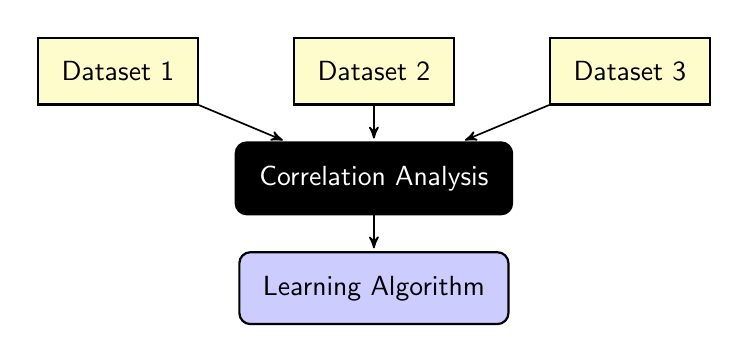
\begin{tikzpicture}[
      font=\sffamily, every matrix/.style={ampersand replacement=\&,column sep=3ex,row
      sep=3ex}, dataset/.style={draw,thick,fill=yellow!20,inner sep=.3cm},
      sink/.style={dataset,rounded corners,fill=black, text=white},
      app/.style={dataset,rounded corners,fill=blue!20}, dots/.style={gray,scale=2},
      to/.style={->,>=stealth',shorten >=1pt,semithick,font=\sffamily\footnotesize}, every
      node/.style={align=center}]

      \matrix{ \node[dataset] (dataset1) {Dataset 1}; \& \node[dataset] (dataset2)
        {Dataset 2}; \& \node[dataset] (dataset3) {Dataset 3}; \\

        \& \node[sink] (blackbox) {Correlation Analysis}; \& \\

        \& \node[app] (application) {Learning Algorithm}; \& \\ };

      \draw[to] (dataset1) -- (blackbox); \draw[to] (dataset2) -- (blackbox); \draw[to]
      (dataset3) -- (blackbox); \draw[to] (blackbox) -- (application);

    \end{tikzpicture}
    \caption{Illustration of multi-modal data fusion}
    \label{fig:data_fusion}
\end{center}
\end{figure}


\section{Canonical Correlation Analysis (CCA)}

\subsection{What is it? What is it not?}

Canonical correlation analysis (CCA) is a joint dimensionality reduction algorithm for
exactly two datasets that finds a linear transformation for each dataset such that the
correlation between the two transformed feature sets is maximized
\cite{hotelling1936relations}. CCA, however, \textit{is not} a data fusion algorithm. CCA
returns two linear transformations and a set of correlations. In this light, CCA is
extremely similar to principle component analysis (PCA), which returns a linear
transformation that accounts for the directions of largest possible variance in a
dataset. These principle components are typically used as features vectors in a variety of
machine learning algorithms. Just as PCA is a dimensionality reduction algorithm and not
the final machine learning algorithm that uses the principle components, CCA is a joint
dimensionality reduction algorithm whose dimensionality reduction ensures that datasets
are maximally correlated in their reduced spaces. These maximally correlated features may
then be used however a learning algorithm desires. 

The solution to CCA is easily found by solving a quadratic optimization problem. This
solution is a closed form expression relying on the singular value decomposition (SVD) of
a matrix product involving the covariance matrices of each dataset and the
cross-covariance between the two datasets. As these covariance matrices are rarely known
\textit{a priori}, practical uses of CCA rely on substituting sample covariance matrices
formed from training data, which we call empirical CCA.

The performance of empirical CCA has been studied previously, but insufficiently. When the
number of training samples is large compared to the dimensions of the datasets, the
performance is well understood \cite{gunderson1997estimating}. When the number of training
samples is less than the sum of the dimension of each dataset (sample deficient regime),
\cite{pezeshki2004empirical} proves that empirical CCA completely breaks down and always
reports a perfect correlation between the datasets. 

This extremely undesirable characteristic of empirical CCA has lead many to abandon CCA as
a reliable statistical analysis technique. Pezeshki, L.L. Scharf et al. argue that in this
sample deficient regime
\begin{quote}
  ... the \textcolor{red}{empirical canonical correlations are defective and
    may not be used} as     estimates of canonical correlations between random
  variables.\cite{pezeshki2004empirical}
\end{quote}
Similarly, Ge et al. conclude that
\begin{quote}
... CCA provide(s) \textcolor{red}{reliable information} about spatial
    correlations existing among pairs of data sets \textcolor{red}{only when SNRs ... are
    reasonably high, and the sample support is significantly larger than the data
    dimensions.}\cite{ge2009does}
\end{quote}



\subsection{Variations on CCA}

Due to this undesirable breakdown of CCA in the low-sample high-dimensionality regime,
many researchers proposed variations of CCA to avoid this performance loss. Most notably,
\cite{nadakuditi2011fundamental} used recent results from random matrix theory to
demonstrate that this performance breakdown may be avoided by trimming the sample
covariance matrix estimates to only include informative components. This algorithm is the
crux of this thesis. We will study its performance and develop theoretical tools in order
to use it for real-world applications. Throughout the thesis, we use the ubiquitous
low-rank signal-plus-noise model for datasets \be X = UV^H + Z, \ee where
$X=[x_1,\dots,x_n]$ is our observed data matrix whose columns are individual
multidimensional observations, $U$ is a low-rank signal subspace, $V$ is a low-rank signal
matrix, and $Z$ is a noise matrix. Surprisingly, correlation analysis for this classical
low-rank signal-plus-noise model is not completely studied. This thesis seeks to complete
the discussion. Here, we briefly touch on other variations based on CCA that do not assume
the above linear low-rank signal-plus-noise model. Many of these algorithms are tuned for
a specific application or seek to avoid the performance loss of CCA in a certain regime.

Regularized CCA (RCCA) \cite{vinod1976canonical} adds a penalty term to the magnitude of
the canonical vectors. This results in adding a scaled copy of the identity matrix to the
sample covariance matrix of each dataset, which allows each matrix to be
inverted. Therefore, RCCA returns non-trivial results in the sample-deficient
regime. However, this approach introduces a parameter to the algorithm; the effect of this
parameter is not well studied. Other variations of RCCA, such as supervised
RCCA \cite{thum2014supervised}, fast RCCA \cite{cruz2014fast}, and a multi-block RCCA
\cite{tenenhaus2014regularized}, have also been proposed.

Kernel CCA (KCCA) \cite{akaho2006kernel} was proposed to deal with non-linear correlations
existing between datasets. However, KCCA also introduces regularization parameters so as
to not return trivial solutions (see \cite{welling2005kcca} for an excellent
derivation). Besides the choice of regularization parameter, there is also ambiguity in
the choice of the kernel function, which is a common problem among kernel methods. Other
variations of KCCA have also been proposed, such as penalized KCCA
\cite{waaijenborg2009correlating}, alpha-beta divergence \cite{mandal2013non}, and CCA
based on kernel target alignment \cite{chang2013canonical}. 

Sparse CCA \cite{hardoon2011sparse} finds linear transformations such that the number of
features used is minimized. This problem is often motivated by the need for interpretable
canonical vectors that is often driven by the application, such as in brain imaging
\cite{yan2014accelerating}. There are many variations on sparse CCA, typically motivated
by application or mathematical intrigue. Sun and Keates \cite{sun2013canonical} explore
CCA in the context of censoring, Shin and Lee examine sparse functional data
\cite{shin2015canonical}, Tao et al. consider joint sparse data in
\cite{tao2014exploring}, Gao et al. explore efficient sparse CCA for high-dimensional
data \cite{gao2014efficient}, and Zhang et al. extend the analysis to multi-class group
sparse CCA \cite{zhang2013binary}. Other formulations include a penalized decomposition
\cite{witten2009penalized}, Bayesian CCA via group sparsity \cite{klami2013bayesian}, and
recursive sparse CCA \cite{chu2013sparse}.

\subsection{Applications}

CCA and its variants are widely used in a variety of fields where multiple datasets
naturally arise, the most common of which is machine learning and computer vision. In
\cite{hardoon2004canonical}, CCA is used to learn semantics of multimedia content by
fusing image and text data. Related, \cite{dhillon2011multi} uses CCA to learn word
embeddings for supervised natural language processing tasks. CCA has been widely applied
to pose estimation \cite{melzer2001nonlinear,zhai2015instance}, as this is a natural
examples where we have multiple views (image) of the same object. Other computer vision
related tasks where correlation methods are natural fits include matching people across
cameras \cite{lisanti2014matching}, clustering social event images
\cite{ahsan2014clustering}, automatic image annotation \cite{hardoon2006correlation}, and
audio-visual speaker clustering \cite{chaudhuri2009multi}.

Medical analysis is another field where there are ripe opportunities for correlation
analysis due to the vast number of modalities (EEG, MRI, CT, fMRI, MEG, etc.). CCA is
often used to determine interactions, or connectivities, between brain areas in fMRI data
\cite{deleus2011functional,arbabshirani2010comparison,khalid2013improving,guccione2013functional}
and used to fuse fMRI, sMRI, and EEG data \cite{correa2010canonical}. CCA based methods
have also been used to examine genetic connections
\cite{lin2013identifying,seoane2014canonical,lin2013group}, relying heavily on sparse
methods due to the high dimensionality of gene data and need to interpret which genes are
``on''. CCA is also a popular way to detect frequencies in steady-state visual evoked
potential (SSVEP) in brain-computer interfaces (BCIs)
\cite{zhang2013l1,nakanishi2014enhancing,zhang2014frequency}. Still further, CCA is used
in de-noising and analysis of EEG, MEG and ECG data
\cite{spuler2013spatial,campi2013non,chen2014removal,kuzilek2014comparison}.

CCA also has roots in classical signal processing applications. The authors of
\cite{via2005canonical} apply CCA to to the common communications problem of blind
equalization of single-input multiple-output (SIMO) channels. Pezeshki et al.
\cite{pezeshki2006canonical} showed that the CCA coordinates are the correct coordinates
for low-rank Gauss-Gauss detection and estimation. Scharf and Thomas
\cite{scharf1998wiener} provide a wonderful exposition on using the canonical coordinates
for Wiener filters, transform coding, filtering, and quantizing. CCA and multiset CCA have
been used to achieve joint blind source separation (BSS) in \cite{li2009joint}. CCA has
also been applied to hyperspectral imaging \cite{nielsen2002multiset}, array processing
\cite{ge2009does}, Gaussian channel capacity \cite{scharf2000canonical}, and cognitive
radio networks \cite{manco2014kernel}.

Other fun and interesting applications include climatology, finance, and music. Todros and
Hero define a new measure transformed based CCA and show its utility on financial data in
\cite{todros2012measure}. Torres et al. \cite{torres2007finding} use sparse CCA to label
portions of musical songs with meaningful words or phrases. In the field of climatology,
CCA has been used to study sea temperatures \cite{wilks2014probabilistic}, forest planning
\cite{prera2014using}, and tropical cyclones \cite{steward2014assimilating}. Finally, I
would be remiss if I didn't share my personal favorite application of CCA to date: using
CCA to analyze bovine growth \cite{li2010canonical}.

\section{Contributions of this thesis}

In many of the application presented above, researchers either have access to many
samples, or have designed an algorithm tuned specifically for a their particular
application. This thesis considers the performance of empirical correlation algorithms in
the low-sample, high dimensional setting. These algorithms are not geared toward a
particular application but are general and may be applied to any application. We will
demonstrate, both theoretically and empirically, that multi-modal correlation analysis in
this regime is a possibility. We remark that statements labeled as theorems represent, to
the best of our knowledge, new results while important results from literature are labeled
as propositions or lemmas. Chapters II-III are self contained and may be read
independently. Chapters IV-X consider the problem of correlation analysis.

Chapters \ref{sec:chpt_msd} and \ref{sec:chpt_msd_exten} consider the classical problem of
matched subspace detectors. We use insights from random matrix theory on the accuracy of
subspace estimates to derive new, optimal detectors that demonstrate the sub-optimality of
the classical plug-in detectors that simply substitute maximum likelihood estimates for
unknown parameters. Under both a stochastic and deterministic data model, we argue that
only the \textit{informative} subspace components should be used in a detector. We extend
this analysis to the case where our observations may contain missing data.

In Chapters \ref{sec:chpt_cca_det} and \ref{sec:chpt_cca_vects}, we explore the
performance of CCA and re-derive informative CCA (ICCA). We demonstrate the extreme
sub-optimality of CCA in the low-sample, high dimensionality regime. Specifically, we
provide a statistical test for both CCA and ICCA that determines whether the correlations
returned by the algorithms do indeed represent a true underlying correlation in the
datasets. We prove when each of these statistics are consistent to showcase the
superiority of ICCA. We also provide an analogous statistical test and consistency theorem
to use when the datasets have missing data entries. We create 3 new real-world,
multi-modal datasets involving video and audio to verify the performance of ICCA. We then
showcase that the canonical vectors returned by ICCA are more accurate than the CCA
vectors in the low-sample regime. Finally, we provide a new algorithm for estimating the
canonical vectors that asymptotically optimal.

Next, we explore the performance of regularized CCA (RCCA) in Chapter
\ref{sec:chpt_rcca}. When the number of training samples is limited but correlation
analysis is still desired, a common strategy is to regularize CCA by adding a penalty to
the magnitude of the linear transformation. However, we demonstrate that setting the
regularization parameter to infinity results in the best performance. In fact, in this
setting, the solution to RCCA may be found by taking the SVD of the sample
cross-covariance matrix between the two datasets. We then predict the behavior of the
largest singular values of this cross-covariance matrix assuming a low-rank
signal-plus-noise model on the individual datasets. We argue that using the top singular
values of this cross-covariance matrix to detect correlations is sub-optimal because the
correlation coefficients are coupled with the individual data signal strengths.

Using a similar proof technique, we predict the behavior of the largest singular values of
the projection of low-rank signal plus noise matrices to a smaller dimension in Chapter
\ref{sec:chpt_svd_proj}. Specifically, we consider two types of projection matrices: one
with standard complex Gaussian entries and one with orthonormal columns. We are able to
provide a closed form expression for the largest singular values in the case where the
projection matrix is unitary. Through numerical simulations, we demonstrate the
superiority of the unitary projection matrix over the Gaussian projection matrix. The
unitary projection matrix can reliably detect the signals at a lower signal-to-noise ratio
than the Gaussian projection matrix. 

In Chapter \ref{sec:chpt_det_reg} we apply CCA and ICCA to the classical problems of
detection and regression. First, we consider the low-rank signal-versus-noise subspace
detection problem given two datasets. We prove that the standard likelihood ratio test
(LRT) detector may be written using the canonical basis returned by CCA. We show that when
using empirical parameter estimates, the CCA detector is extremely suboptimal but that the
ICCA detector is equivalent to the plug-in LRT detector. We then show that the classical
Gaussian regression problem may be written in terms of the CCA basis. However, similar to
the detection problem, empirical CCA degrades the performance significantly while ICCA
matches the classical plug-in detector. We show this via mean squared error prediction
plots.

We then consider the joint problems of image retrieval and image annotation in Chapter
\ref{sec:chpt_ia}. Correlation based methods are typically overlooked as solutions to such
problems due to the problems with CCA outlined in this thesis. We show that using ICCA to
solve these problems results in non-trivial solutions. We compare the performance of CCA
and ICCA on four different image-text datasets and describe the capabilities and
limitations of ICCA in this application. When the datasets contain multiple images of the
same objects and meaningful captions, ICCA is able to capture correlations between images
and text. However, ICCA fails to capture semantic meanings between documents and
captions. We argue that with clever feature engineering and improved NLP techniques,
correlation based methods may be relevant for image retrieval and image annotation.

Lastly, we consider multi-set CCA (MCCA) in Chapter \ref{sec:chpt_mcca}. Unfortunately,
unlike CCA, there is no clear objective function to use in an optimization problem;
Kettenring \cite{kettenring1971canonical} proposes five such objective functions. Nielsen
also provides a nice formulation of MCCA in \cite{nielsen1994analysis} where he proposes
four constraint functions.  We provide derivations for these 20 formulations, in both a
theoretical and empirical setting. We then choose to consider the MAXVAR problem as we are
able to directly apply our insights from ICCA to create an informative version of it,
which we call informative MCCA (IMCCA). We demonstrate the superior performance of IMCCA
on a real-world video dataset that we created. 



\chapter{Performance of Matched Subspace Detectors Using Finite Training Data}
%\documentclass[draftcls,peerreview,onecolumn]{IEEEtran}
\documentclass[10pt,twocolumn,twoside]{IEEEtran}

\usepackage{amstext}
\usepackage{amsmath}
\usepackage{amssymb}
\usepackage{graphicx}
\usepackage{epstopdf}
\usepackage{algorithm}
\usepackage{algorithmic}
\usepackage{booktabs}
\usepackage{subfigure, comment, color}

% correct bad hyphenation here
\hyphenation{op-tical net-works semi-conduc-tor}

\input IEEE_RMT_MSD_header.tex

\begin{document}
%
% paper title
% can use linebreaks \\ within to get better formatting as desired
\title{The Performance of a Matched Subspace Detector that Uses Subspaces Estimated from Finite, Noisy, Training Data}


\author{Nicholas~Asendorf*
        and~Raj~Rao~Nadakuditi\\
EDICS: SSP-DETC, SSP-PERF% <-this % stops a space

\thanks{N. Asendorf is with the Department
of Electrical Engineering and Computer Science, 1301 Beal Avenue, Room 4313, University of Michigan, Ann Arbor,
MI, 48109 USA (e-mail: asendorf@umich.edu).}% <-this % stops a space
\thanks{R.R. Nadakuditi is with the Department
of Electrical Engineering and Computer Science, 1301 Beal Avenue, Room 4118, University of Michigan, Ann Arbor,
MI, 48109 USA (e-mail: rajnrao@umich.edu).}% <-this % stops a space
\thanks{Manuscript received ??}}




% The paper headers
\markboth{IEEE Journal,~Vol.~?, No.~?, ?~?}%
{Asendorf and Nadakuditi: The Performance of a Matched Subspace Detector that Uses Subspaces Estimated from Finite, Noisy, Training Data}
% The only time the second header will appear is for the odd numbered pages
% after the title page when using the twoside option.
%
% *** Note that you probably will NOT want to include the author's ***
% *** name in the headers of peer review papers.                   ***
% You can use \ifCLASSOPTIONpeerreview for conditional compilation here if
% you desire.

% make the title area
\maketitle


\begin{abstract}
We analyze the performance of a matched subspace detector (MSD) where the test signal vector is assumed to reside in an unknown, low-rank $k$ subspace that must be estimated from finite, noisy, signal-bearing training data. Under both a stochastic and deterministic model for the test vector, subspace estimation errors due to limited training data degrade the performance of the standard plug-in detector, relative to that of an oracle detector. To avoid some of this performance loss, we utilize and extend recent results from random matrix theory (RMT) that precisely quantify the quality of the subspace estimate as a function of the eigen-SNR, dimensionality of the system, and the number of training samples. We exploit this knowledge of the subspace estimation accuracy to derive from first-principles a new RMT detector and to characterize the associated ROC performance curves of the RMT and plug-in detectors. Using more than the a critical number of \textit{informative} components, which depends on the training sample size and eigen-SNR parameters of training data, will result in a performance loss that our analysis quantifies in the large system limit.  We validate our asymptotic predictions with simulations on moderately sized systems.

\end{abstract}

% Note that keywords are not normally used for peerreview papers.
\begin{IEEEkeywords}
Matched subspace detector, deterministic, stochastic, random matrix theory, ROC analysis
\end{IEEEkeywords}


\IEEEpeerreviewmaketitle

\section{Introduction}\label{sec:intro}
\textcolor{blue}{\IEEEPARstart{M}{any} signal processing  \cite{scharf1991statistical} and machine learning \cite{friedman2001elements} applications involve the task of detecting a signal of interest buried in high dimensional noise. A matched subspace detector (MSD) is commonly used to solve this problem when the target signal is assumed to lie in a low-rank subspace.  The low-rank signal buried in noise model is ubiquitous in signal processing. See for example, \cite{besson2006cfar,bandiera2007glrt, bandiera2007adaptive}, which determine if a snapshot is noise-only or if it contains target echoes, \cite{maris2003resampling, soong1995principal}, which examine source localization in electroencephalography (EEG) and magnetoencephalography (MEG) data, and \cite{besson2005matched}, which examines low-rank signal recovery in radar, sonar, and communications applications. The performance of such detectors when the signal subspace is known a priori has been extensively studied (see, for example, \cite{besson2006cfar,scharf1994matched,jin2005cfar,mcwhorter2003matched, vincent2008matched} to list a few). This paper considers the performance of a MSD in the less studied setting where the signal subspace is unknown and must be estimated from finite, noisy, signal-bearing training data.}

\textcolor{blue}{The setting we have in mind arises from machine learning related applications where the low-rank signal model is reasonable but the signal subspace is not parameterizable. This is in contrast to the array processing applications that motivated the original MSD work \cite{scharf1994matched} where the signal subspace is explicitly parameterizable whenever the array geometry is known. The inferential problem is made tractable by the availability of a training dataset consisting of signal-bearing observations that have been collected in a variety of representative experimental (and thus noisy) conditions. In such a scenario,  the truncated eigen-decomposition of the sample covariance matrix of this training data yields an estimate of the unknown low-rank signal subspace, which may then be used for signal versus noise discrimination.}

\textcolor{blue}{An illustrating example of this is the classical problem of handwriting recognition \cite[Chapter 10]{elden2007matrix} where a MSD can be used to determine if an area of an image contains a digit $0-9$ or is pure noise. Here, a database \cite{hwritingurl}, containing a large number of handwritten samples of each of the digits written by many different writers, is used to form a low-rank subspace estimate of each digit. The samples are noisy because of digitization effects and the inherent variation between writers. A nearest-subspace classifier based on retaining only the first few ($10-12$, in this example) principal components (or leading eigenvectors of the digit's training data sample covariance matrix) associated with each digit yields greater than 93\% classification performance \cite[Table 10.1, pp. 121]{elden2007matrix}, indicating that the low-rank signal buried in noise model is appropriate. The motivating setting described also arises in the context of image or wavefront recognition applications (e.g. license plate character recognition) where the target and the camera are separated by a dynamic random medium and in hyperspectral imaging based anomaly detection  \cite{thai2002invariant,healey1999models,kwon2006kernel} relative to a statistically stationary scene (e.g. toxic gas detection). Here too, a practitioner might have access to training samples collected over a variety of experimental conditions and might employ the MSD in a similar manner.}

\textcolor{blue}{In these applications, the standard plug-in detector, which substitutes an estimate of the signal subspace into the expression for the oracle MSD that was derived assuming the subspace is perfectly known, realizes a performance loss because additive noise and finite training data decrease the accuracy of the estimated subspace. This motivates questions such as: What is the expected plug-in detector performance? Is it possible to avoid some of this performance loss? How does the estimation of the signal subspace dimension influence detector  performance? Is the ``play-it-safe''  overestimation of subspace dimension, to compensate for the potential underestimation of schemes discussed in \cite{nadakuditi2008sample} , a good idea? }

\textcolor{blue}{Our performance analysis, which relies on insights from random matrix theory (RMT), highlights the importance of using no more than $\keff$ \textit{informative} signal subspace components, where $\keff$ is a number that depends on the system dimensionality, number of training samples, and eigen-SNR (signal-to-noise-ratio). We derive a new RMT detector that only utilizes the $k_\text{eff}$ \textit{informative} signal subspace components, thereby avoiding some of the possible performance loss suffered by the plug-in detector. Given the number and quality (i.e. SNR) of the training samples, our analysis also allows a practitoner to predict the expected receiver operating characteristic (ROC) performance of a general class of detectors. An outcome of this analyis is that we can accurately predict how many training samples are needed to get to within $\epsilon$ of the oracle MSD's performance (see Figures \ref{fig:epsilon_graph}, \ref{fig:stoch_theory_epsilon}, and \ref{fig:determ_theory_epsilon}). This performance characterization can provide the practitioner with experimental guidance and might be a starting point for the formulation of achievable system performance specifications.}

\textcolor{blue}{This paper differs from previous works in several aspects. The focus and main contribution is analytically quantifying the performance of a general class of MSD's as a function of the system dimensionality, number of training samples, and eigen-SNR. Theorem \ref{th:other angles} and Corollary \ref{corr:matrix} extend recent results from RMT \cite{paul2007asymptotics,benaych2011eigenvalues, benaych2011singular} to precisely quantify the accuracy of the subspace estimate. This quantification yields approximations that appear to hold for moderate system dimensions even though the theory is asymptotic, in the limit of large dimensionality and relatively large training sample size. We provide a first-principles derivation of a new RMT detector that incorporates this knowledge of the accuracy of the estimated subspace, thereby illuminating the asymptotic form of a detector that mitigates some of the potential performance loss suffered by the plug-in detector. These RMT insights also allow us to characterize the ROC performance of a MSD under both a deterministic and stochastic model for the test vector. This work builds on \cite{asendorf2011msd} by providing the proofs of Theorem \ref{th:other angles} and Corollary \ref{corr:matrix}, analyzing the performance of the general class of detectors given in (\ref{eq:detector_form}), considering the deterministic test vector setting, and unifying the performance analysis of the stochastic and deterministic MSD's.}

\textcolor{blue}{The paper is organized as follows. We describe the generative models for the training data and test vector and also estimate unknown parameters in Section \ref{sec:data_models}. In Section \ref{sec:std_detecs}, we derive standard oracle and plug-in detectors for each testing setting and highlight how finite training data causes subspace estimation errors and subsequent performance loss. We formally pose the questions addressed herein in Section \ref{sec:prob_state}. Section \ref{sec:rmt} contains pertinent results from RMT and our definition in (\ref{eq:keff}) of $\keff$. In Section \ref{sec:rmt_detecs} we derive RMT detectors for the stochastic and deterministic test vector models. Aided by RMT and a saddlepoint approximation of the CDF of a weighted sum of chi-square random variables, we predict ROC performance curves for a general detector in Section \ref{sec:roc_theory}. We validate our asymptotic ROC predictions and demonstrate the importance of using the $k_\text{eff}$ informative subspace components in Section \ref{sec:results}. We provide concluding remarks in Section \ref{sec:conclusion}.}







\section{Problem Statement}\label{sec:prob_state}
\subsection{Training Data Model}\label{sec:training_data}We are given
  $m$ signal-bearing training vectors $y_i\in \complex^{n\times 1}$, $i=1,\dots,m$, modeled\footnote{For expositional simplicity, we have assumed that all our matrices and vectors are complex-valued; our results also hold for real-valued matrices and vectors.} as $y_i=Ux_i+z_i$ where $z_i\overset{\text{i.i.d.}}{\sim}\mathcal{CN}(0,I_n)$, $U$ is an unknown $n\times k$ complex matrix with orthonormal columns, and $x_i\overset{\text{i.i.d.}}{\sim}\mathcal{CN}(0,\Sigma)$ where $\Sigma=\diag(\sigma_1^2,\dots,\sigma_k^2)$ with $\sigma_1>\sigma_2>\dots>\sigma_k>0$ unknown. For each observation, $x_i$ and $z_i$ are independent. The dimension, $k$, of our subspace is unknown and we assume throughout that $k\ll n$ so that we have a low-rank signal embedded in a high-dimensional observation vector.

  Given a dimension estimate, $\widehat{k}$, and the signal bearing training data $Y = \begin{bmatrix} y_1 & \dots & y_m \end{bmatrix}$, we form a subspace estimate $\widehat{U}\in\complex^{n\times\widehat{k}}$ by taking the leading $\widehat{k}$ eigenvectors of $YY^{H}/m$ and a signal covariance estimate $\widehat{\Sigma}\in\reals^{\widehat{k}\times\widehat{k}}$ (in a manner to be specified).

\subsection{Testing Data Model}
We will consider two models for the test vectors. In the stochastic setting, the test vector $y\in\complex^{n\times 1}$ is modeled as
\begin{equation}\label{eq:stoch_setup}
\text{Stochastic Model: }y=\left\{
\begin{aligned}
&z
&& y\in H_0:\text{ Noise only}\\
&Ux+z
&& y\in H_1:\text{ Signal-plus noise}\\
\end{aligned}\right. ,
\end{equation}
where $U$, $z$, and $x$ are modeled as described in Section \ref{sec:training_data}. This assumes that the signal, $Ux$, may lie anywhere in the subspace and whose position in the subspace is governed by the signal covariance matrix $\Sigma$.

In the deterministic setting, the test vector $y\in\complex^{n\times 1}$ is modeled as
\begin{equation}\label{eq:determ_setup}
\text{Deterministic Model: }y=\left\{
\begin{aligned}
&z
&& y\in H_0:\text{ Noise only}\\
&U\Sigma^{1/2} x+z
&& y\in H_1:\text{ Signal-plus noise}\\
\end{aligned}\right. ,
\end{equation}
where $U$, $\Sigma$, and $z$ are modeled as before. Here, in contrast to the stochastic setting, $x$ is a non-random deterministic vector. Thus the signal, $U\Sigma^{1/2}x$, lies at a fixed point in the unknown subspace. Note that placing a mean zero, identity covariance Gaussian prior on $x$ in (\ref{eq:determ_setup}) yields the stochastic model described in (\ref{eq:stoch_setup}).

\subsection{Problem 1: Characterize the ROC Performance Curves}\label{sec:problem 1}
Given an independent test observation from (\ref{eq:stoch_setup}) or (\ref{eq:determ_setup}), we first use $\widehat{U}$ to generate a $\widehat{k}\times 1$ test vector $w=\widehat{U}^Hy$. The vector $w$ is a sufficient statistic \cite{scharf1991statistical} when $\widehat{U} = U$. We focus on detectors of the form
\begin{equation}\label{eq:detector_form}
w^HDw\detgtrless\eta,
\end{equation}
where $D$ is a diagonal matrix and the test statistic $\Lambda(w) := w^HDw$ is compared against a threshold, $\eta$, set to achieve a prescribed false alarm rate $\alpha$. For detectors of this form and for test vectors modeled as (\ref{eq:stoch_setup}) or (\ref{eq:determ_setup}), our goal is to
\begin{center}
Predict $P_D=:\mathbb{P}(\text{Detection})$, for every $P_F:=\alpha \in (0,1)$ given $n$, $m$, $\widehat{k}$, $D$ and $\Sigma$.
\end{center}

This performance prediction relies on RMT results quantifying the accuracy of the subspace estimate $\widehat{U}$ as a function of the parameters listed.
%We will consider detectors, $g(w)\to\{H_0,H_1\}$, which solve
%\begin{equation}\label{eq:maximization}
%\begin{aligned}
%&\text{maximize}
%&& P_D=P\left(g(w)\to H_1 | w\in H_1\right)\\
%&\text{subject to}
%&& P_F=P\left(g(w)\to H_1 | w\in H_0\right)\leq\alpha\\
%\end{aligned}
%\end{equation}
%where $\alpha\in[0,1]$.

\subsection{Problem 2: Derive and Predict the Performance of a Detector that Exploits  Predictions of Subspace Accuracy}\label{sec:ps_prob2}
In the  Neyman-Pearson setting (see \cite{van1968detection}), a MSD is a likelihood ratio test (LRT) taking the form
\begin{equation*}
\Lambda(w):=\dfrac{f(w|H_1)}{f(w|H_0)} \detgtrless \eta
\end{equation*}
where $\Lambda(w)$ is the test statistic, $\eta$ is the threshold set to achieve a given false alarm rate, and $w = \widehat{U}^{H}y$. Here, $\widehat{U}$ is a noisy estimate of the underlying $U$; its accuracy, relative to $U$, can be quantified using RMT. Therefore, $f(w|H_0)$ and $f(w|H_1)$, and consequently $\Lambda(w)$, depend on the `noisiness' of the estimated subspaces.  Our goal is thus to
\begin{quote}
Design \& analyze the performance of  a detector that exploits RMT predictions of subspace estimation accuracy.
\end{quote}
The design and performance prediction aspect of this problem will provide insights on when, if, and how the performance of plug-in detectors that do not exploit the knowledge of subspace estimation accuracy can be improved.


%and we employ the generalized likelihood ratio test (GLRT). It is standard to substitute estimates $\widehat{U}$  and $\widehat{\Sigma}$ for the unknown $U$ and $\Sigma$ in the oracle test statistic \cite{jin2005cfar,mcwhorter2003matched}. This resulting plug-in detector assumes that the parameter estimates are exact. Through our analysis, we characterize the performance loss associated with making this assumption and derive a new detector which can systematically avoid this performance loss. By relying on the subspace accuracy estimates presented in Theorem \ref{th:angles}, the new RMT detector only utilizes $\min(\widehat{k},k_\text{eff})$ subspace components to form an approximation to the oracle detector. In both testing scenarios, the plug-in and RMT detectors take the desired form of (\ref{eq:detector_form}).


\section{Pertinent Results from Random Matrix Theory}\label{sec:rmt}
In Section \ref{sec:param_estim} we formed estimates $\widehat{U}$ and $\widehat{\Sigma}$ of the unknown $U$ and $\Sigma$ by taking the eigen-decomposition of the sample covariance matrix $S$ of the training data matrix $Y$. These estimates are inaccurate because the training data is noisy and contains only a finite number of observations. The following analysis specifically quantifies the accuracy of these estimates and is necessary to derive a new detector and predict ROC performance curves of detectors with the form of (\ref{eq:detector_form}).

\subsection{Eigenvector Aspects}\label{sec:eigvect_aspects}

The subspace estimate $\widehat{U}$ is formed from the eigenvectors corresponding to the $\widehat{k}$ largest eigenvalues of $S$. For an arbitrary non-random diagonal matrix $D$, we will be particularly interested in the matrix $\widehat{U}^HUDU^H\widehat{U}$ that appears in detector derivations and the ROC performance analysis in Sections \ref{sec:rmt_detecs} and \ref{sec:roc_theory}. The following proposition characterizes the limiting behavior (up to an arbitrary phase) of the diagonal entries of the matrix $\widehat{U}^HU$.

\begin{prop}\label{th:angles}
Assume that the columns of the training data matrix $Y$ were generated as described in Section \ref{sec:training_data}. Let $\widehat{u}_{i}$ denote the eigenvector associated with the $i$-th largest eigenvalue of $S$. Then for $i = 1, \ldots, k$ and $n, m \longrightarrow \infty$ with $n/m \to c$, we have that
\begin{equation}\label{eq:angles}
|\langle u_i,\widehat{u}_i\rangle|^2 \convas
\begin{cases}
\dfrac{\sigma_i^4-c}{\sigma_{i}^4+\sigma_{i}^2c} & \text{ if } \sigma_{i}^2>\sqrt{c}\\
0 & \textrm{otherwise}\\
\end{cases}.
\end{equation}
\end{prop}
\begin{proof}
This follows from Theorem 4 of \cite{paul2007asymptotics} when $\gamma=c$, $\ell_\nu-1=\sigma_\nu^2$, $\widetilde{e}_\nu=u_v$, and $p_\nu=\widehat{u}_\nu$. This result also appears in Theorem 2.2 of \cite{benaych2011eigenvalues}.
\end{proof}

We note that $\convas$ denotes almost sure convergence. The key insight from Proposition \ref{th:angles} is that only the eigenvectors corresponding to the signal variances, $\sigma_i^2$, lying above the phase transition $\sqrt{c}$ are \textit{informative}. When a signal variance drops below this critical threshold, the corresponding eigenvector estimate is essentially noise-like  (i.e. $|\langle u_i,\widehat{u}_i\rangle|^2=o_{p}(1)$ meaning $|\langle u_i,\widehat{u}_i\rangle|^2\overset{p}{\to}0$ as $n\to\infty$, denoting convergence in probability) and thus \textit{uninformative}. Decreasing the amount of training data, $m$, increases $c$, thereby decreasing the value of $|\langle u_i,\widehat{u}_i\rangle|^2$; if this quantity became $0$, the associated subspace component would become uninformative.

The term $|\langle u_i,\widehat{u}_i\rangle|^2$ quantifies mismatch between the estimated and underlying eigenvectors and will play an important role in deriving a new RMT detector and in characterizing detector performance; a similar term also appears in the analysis of the resolving power of arrays due to model mismatch such as in \cite{cox1973resolving}.


Following \cite{nadakuditi2008sample}, we define the effective number of (asymptotically) identifiable subspace components $k_\text{eff}$ as:
\begin{equation}\label{eq:keff}
\boxed{k_\text{eff} = \text{Number of } \sigma_i^2 > \sqrt{c}}.
\end{equation}
We can form an estimate of $k_\text{eff}$, $\widehat{k}_{\text{eff}}$, using  `Algorithm 2' of  \cite{nadakuditi2010fundamental}. This algorithm assumes the same model of a low-rank signal buried in high dimensional noise as our training data. Given a desired significance level, the algorithm estimates the number of signals present in a finite number of samples. When the noise covariance matrix is not known a priori, we would instead use `Algorithm 1' of \cite{nadakuditi2010fundamental}. Both algorithms rely on the Tracy-Widom distribution. Note that $\widehat{k}_{\text{eff}} \leq k$ but that we allow $\widehat{k} \geq \widehat{k}_{\text{eff}}$ so we may understand the impact of a play-it-safe overestimation of the signal subspace dimension estimate $\widehat{k}_{\text{eff}}$  returned using RMT based detectors \cite{nadakuditi2010fundamental,johnstone2001distribution,el2007tracy}.

Proposition \ref{th:angles} only characterizes the limiting behavior (up to an arbitrary phase) of  the diagonal entries of the matrix $\widehat{U}^HU$. We now state a new theorem characterizing the limiting behavior of the off-diagonal entries in $\widehat{U}^HU$.

\begin{Th}\label{th:other angles}
Assume the same hypothesis as in Proposition \ref{th:angles}. Let $\widehat{k}=\keff=k$. For $i=1,\dots,\widehat{k}$, $j=1,\dots,k$, and $i\neq j$, as $n,m\to\infty$ with $n/m\to c$, $\langle u_j,\widehat{u}_i\rangle \convas 0.$
\end{Th}
\begin{proof}
This is a new result. See Appendix for proof.
\end{proof}\vskip0.25cm

\begin{Conj}\label{conj:angles}
Assume the same hypothesis as in Proposition \ref{th:angles}. For $i=1,\dots,\widehat{k}$, $j=1,\dots,k$, and $i\neq j$, as $n,m\to\infty$ with $n/m\to c$, $\langle u_j,\widehat{u}_i\rangle \convas 0$.
\end{Conj}
\begin{Remark}
See Appendix for a brief discussion of this claim.
\end{Remark}

Together, Proposition \ref{th:angles} and Claim \ref{conj:angles} characterize the limiting behavior of the entries of $\widehat{U}^HU$. This permits approximation, in the large matrix limit, of  $\widehat{U}^HU D U^H\widehat{U}$ by a suitable diagonal matrix.

\begin{Corr}\label{corr:matrix}
Suppose $\widehat{k}\leq k$ and let $D$ be a $k \times k$ (non-random) diagonal matrix such that $D=\diag(d_1,\ldots,d_{k})$, independent of $\widehat{U}$. Then as $n,m \longrightarrow \infty$ with $n/m \to c$, we have that
\begin{equation*}
\widehat{U}^HU D U^H\widehat{U}\convas \diag(d_1 |\langle u_1,\widehat{u}_1\rangle|^2,\dots, d_{\widehat{k}} |\langle u_{\widehat{k}},\widehat{u}_{\widehat{k}}\rangle|^2)
\end{equation*}
where for $i=1,\dots,\widehat{k}$ the quantity $|\langle u_i,\widehat{u}_i\rangle|^2$ is given in Proposition \ref{th:angles}.
\end{Corr}
\begin{proof}
This follows directly by applying Proposition \ref{th:angles} and Claim \ref{conj:angles} to the entries of the matrix $U^H\widehat{U}$.
\end{proof}

This diagonal approximation of $\widehat{U}^HU D U^H\widehat{U}$ will be used in detector derivations and ROC performance analyses in Sections \ref{sec:rmt_detecs} and \ref{sec:roc_theory}.

\subsection{Eigenvalue Aspects}

The signal covariance estimate $\widehat{\Sigma}$ is formed from the largest $\widehat{k}$ eigenvalues of $S$. To characterize the ROC performance curves of plug-in detectors that use $\widehat{\Sigma}$ as the signal covariance estimate, we will also need to characterize the limiting behavior of $\widehat{\Sigma}$.  The following proposition gives the limiting behavior of these signal variance estimates.
\begin{prop}\label{th:eigvals_rmt}
As $n,m \longrightarrow \infty$ with $n/m \to c$ we have that:
\begin{equation*}
\widehat{\sigma}_i^2\convas
\begin{cases}
 \sigma_i^2 + c + \frac{c}{\sigma_i^2} & \text{ if } \sigma_i^2 > \sqrt{c}\\
 c + 2\sqrt{c} & \text{ if } \sigma_i^2 \leq \sqrt{c}
\end{cases}.
\end{equation*}
\end{prop}
\begin{proof}
This follows from Theorems 1 and 2 in \cite{paul2007asymptotics} for the real setting for $c<1$ when $\gamma=c$, $\ell_\nu-1=\sigma_\nu^2$, and $\widehat{\ell}_\nu -1 = \widehat{\sigma}_\nu^2$. See Theorem 2.6 in \cite{benaych2011singular} for the complete result.
\end{proof}
These limiting values will be used in Section \ref{sec:roc_theory} when deriving the ROC performance of the plug-in detectors.

When only finite training data is available, $c$ is non-zero and Proposition \ref{th:eigvals_rmt} shows that $\widehat{\sigma}_i^2$ is biased. We wish to derive an improved signal variance estimate to use in a new RMT detector and to estimate $|\langle u_i,\widehat{u}_i\rangle|^2$ in (\ref{eq:angles}). As seen in Proposition \ref{th:angles}, when $\sigma_i^2\leq\sqrt{c}$ the eigenvector estimate is uninformative and we would not want to include that subspace component in a detector; the associated signal variance estimate is therefore unnecessary. For the $\widehat{k}_{\text{eff}}$ subspace components that are informative (i.e. when $\sigma_i^2 > \sqrt{c}$) we form an improved signal variance estimate using the following proposition that characterizes the fluctuations of these signal variance estimates.
\begin{prop}\label{th:eigenvalues}
As $n,m \longrightarrow \infty$ with $n/m \to c$, we have that for $i = 1, \ldots, \keff$
\begin{equation*}
\sqrt{n}\left(\widehat{\sigma}_i^2-\left(\sigma_i^2+c+\frac{c}{\sigma_i^2}\right)\right)\Rightarrow\mathcal{N}\left(0,\frac{2\left(\sigma_i^2+1\right)^2}{\beta }\left(1-\frac{c}{\sigma_i^4}\right)\right),
\end{equation*}
where $\beta = 1$ when the data is real-valued and $\beta = 2$ when the data is complex-valued.
\end{prop}
\begin{proof}
This follows from Theorem 3 in \cite{paul2007asymptotics} for the real setting for $c<1$ when $\gamma=c$, $\ell_\nu-1=\sigma_\nu^2$, $\widehat{\ell}_\nu-1=\widehat{\sigma}_\nu^2$, and $p_\nu$ is the limit of Theorem 2 of \cite{paul2007asymptotics}. See Theorem 2.15 in \cite{benaych2011singular} for the complete result.
\end{proof}
For the $\widehat{k}_{\text{eff}}$ informative subspace components we form an improved estimate, $\widehat{\sigma}^2_{i_\text{rmt}}$, of the unknown signal variance, $\sigma_{i}^{2}$, by employing maximum-likelihood (ML) estimation on the distribution in Proposition \ref{th:eigenvalues}. Specifically, for only the $\widehat{k}_{\text{eff}}$ signal eigenvalues, we form the RMT estimate:
\begin{equation}\label{eq:cov}
\widehat{\sigma}^2_{i_\text{rmt}} = \argmax_{\sigma_i^2} \log\left(f_{\widehat{\sigma}_i^2}(\sigma_i^2)\right)
\end{equation}
where
\begin{equation*}
f_{\widehat{\sigma}_i^2}(\sigma_i^2):=\mathcal{N}\left(\left(\sigma_i^2+c+\frac{c}{\sigma_i^2}\right),\frac{2\left(\sigma_i^2+1\right)^2}{n\beta }\left(1-\frac{c}{\sigma_i^4}\right)\right).
\end{equation*}
We may then estimate $|\langle u_i,\widehat{u}_i\rangle|^2$ in (\ref{eq:angles}) by substituting the improved signal variance estimates, $\widehat{\sigma}^2_{i_\text{rmt}}$, for the unknown $\sigma_i^2$ in Proposition \ref{th:angles}. We refer to this estimate as $|\langle u_i,\widehat{u}_i\rangle|^2_{\text{rmt}}$. For the $\widehat{k}-\widehat{k}_{\text{eff}}$ uninformative subspace components, we set $|\langle u_i,\widehat{u}_i\rangle|^2_{\text{rmt}}=0$.


\section{Family of Stochastic Matched Subspace Detectors}\label{sec:msd_stoch}
We now derive a family of detectors for the stochastic observation vector model in (\ref{eq:stoch_setup}). Recall that we form a test vector $w=\widehat{U}^Hy$; the elements of $w$ are the `co-ordinates' of $y$ in the subspace spanned by the columns of $\widehat{U}$. In the Neyman-Pearson setting, the oracle detector is a LRT which relies on the conditional distributions of our test vector $w$ under each hypothesis. By properties of Gaussian random variables these distributions are simply
\begin{equation}\label{eq:stoch_distr}
\begin{aligned}
&w|H_0\sim\mathcal{N}\left(0,I_{\widehat{k}}\right)\\
&w|H_1\sim\mathcal{N}\left(0, \widehat{U}^HU\Sigma U^H\widehat{U} +I_{\widehat{k}}\right).\\
\end{aligned}
\end{equation}
We obtain a family of detectors by placing various assumptions on the covariance of $w|H_1$, as described next.
%Given a dimension estimate $\widehat{k}$, $\widehat{U}$ is a $n\times\widehat{k}$ matrix formed by stacking the top $\widehat{k}$ eigenvectors of the sample covariance matrix of the training data alongside each other.

\subsection{Oracle Detector}\label{sec:oracle_stoch}
The oracle detector assumes that $k$, $\Sigma$, and $\widehat{U}^{H}U$ are all known in (\ref{eq:stoch_distr}). The LRT statistic is
\begin{equation*}
\Lambda(w)=\frac{\mathcal{N}(0,\widehat{U}^HU\Sigma U^H\widehat{U} + I_k)}{\mathcal{N}(0,I_{k})}.
\end{equation*}
After simplification of this expression using the natural logarithm operator as a monotonic operation, the oracle statistic becomes
\begin{equation}\label{eq:oracle_stat_stoch}
\boxed{\Lambda_{\text{oracle}}(w) = w^H\left[I_k-\left(\widehat{U}^HU\Sigma U^H\widehat{U}+I_k\right)^{-1}\right]w}
\end{equation}
and the oracle detector is
\begin{equation}\label{eq:oracle_class_stoch}
\Lambda_{\text{oracle}}(w) \detgtrless \gamma_{\text{oracle}}
\end{equation}
where the threshold $\gamma_{\text{oracle}}$ is chosen in the usual manner, \ie, so that satisfies $P(\Lambda_{\text{oracle}}(w)>\gamma_{\text{oracle}}|H_0)=\alpha$ with $\alpha$ a desired false alarm rate. We note that the oracle statistic assumes that the matrix $\widehat{U}^HU\Sigma U^H\widehat{U}$ is known. Corollary \ref{corr:matrix} states that in the large system limit, this matrix converges almost surely to a diagonal matrix; we exploit this in Section \ref{sec:optimal_stoch} to address the problem posed in Section \ref{sec:ps_prob2}.

\subsection{Plug-in Detector}\label{sec:plugin_stoch}
When the parameters $\Sigma$ and $U$ (and the implicit variable $k$) in (\ref{eq:stoch_distr}) are unknown, the expression in (\ref{eq:oracle_stat_stoch}) cannot be computed. Suppose that we are provided a dimension estimate $\widehat{k}$ so that we may employ the generalized likelihood ratio test (GLRT) based on the distributions in (\ref{eq:stoch_distr}). The GLRT statistic is
\begin{equation*}
\Lambda(w) = \frac{\max_{U,\Sigma}\mathcal{N}(0,\widehat{U}^HU\Sigma U^H\widehat{U} + I_{\widehat{k}})}{\mathcal{N}(0,I_{\widehat{k}})}.
\end{equation*}
The (classical) ML estimates (in the large-sample, small matrix setting) for $U$ and $\Sigma$ are given by \cite{muirhead1982aspects}
\begin{equation}\label{eq:param_estims_stoch}
\begin{aligned}
&\widehat{U}=[\widehat{u}_1 \dots \widehat{u}_{\widehat{k}}]\\
&\widehat{\sigma}_i^2 = \widehat{\lambda}_i -1 \text{ for } i=1,\dots,\widehat{k}\\
\end{aligned}
\end{equation}
where $\widehat{\lambda}_1,\dots,\widehat{\lambda}_{\widehat{k}}$ are the $\widehat{k}$  largest eigenvalues of the sample covariance matrix, $S$, and $\widehat{u}_1,\dots,\widehat{u}_{\widehat{k}}$ are the corresponding eigenvectors. Define the signal covariance matrix estimate as $\widehat{\Sigma}=\diag(\widehat{\sigma}_1^2,\dots,\widehat{\sigma}_{\widehat{k}}^2)$. We then substitute these ML estimates for the unknown parameters in (\ref{eq:oracle_stat_stoch}) as in \cite{jin2005cfar} and \cite{mcwhorter2003matched}. This results in the following plug-in detector statistic:
\begin{equation*}
\Lambda_{\text{plugin}}(w)= w^H\left(I-\left[\widehat{U}^H\widehat{U}\widehat{\Sigma}\widehat{U}^H\widehat{U} + I\right]^{-1}\right)w.
\end{equation*}
This simplifies to
\begin{equation}\label{eq:plugin_stat_stoch}
\boxed{\Lambda_{\text{plugin}}(w) = w^H\diag\left(\frac{\widehat{\sigma}^2_i}{\widehat{\sigma}^2_i+1}\right)w=\sum_{i=1}^{\widehat{k}}\left(\frac{\widehat{\sigma}_i^2}{\widehat{\sigma}_i^2+1}\right)w_i^2}
\end{equation}
and our detector takes the form
\begin{equation}\label{eq:plugin_class_stoch}
{\Lambda_{\text{plugin}}(w) \detgtrless \gamma_{\text{plugin}}}
\end{equation}
where the threshold $\gamma_{\text{plugin}}$ is chosen in the usual manner. The stochastic plug-in detector clearly takes the form of (\ref{eq:detector_form}).

The plug-in detector assumes that the estimated signal subspace, $\widehat{U}$, is equal to the true signal subspace, $U$, and that the estimated signal covariance, $\widehat{\Sigma}$, is equal to the true signal covariance, $\Sigma$. In other words,  the plug-in detector derivation assumes that $|\langle u_i,\widehat{u}_i\rangle|^2=1$ and $\widehat{\sigma}_i^2=\sigma_i^2$ and that the provided subspace dimension estimate, $\widehat{k}$, is equal to the true underlying dimension of our signal subspace, $k$. Perhaps unsurprisingly, (as discussed in Section \ref{sec:rmt}) choosing $\widehat{k} > k_\text{eff}$ degrades the performance of the plug-in detector. Next we discuss an alternate viewpoint on the optimality of choosing $\keff$ components.

\subsection{Random Matrix Theory Detector}\label{sec:optimal_stoch}
Consider the covariance matrix of the conditional distribution $w|H_1$ in (\ref{eq:stoch_distr}). By Corollary \ref{corr:matrix}, we have that in the large matrix limit
\begin{equation}\label{eq:cov mat}
\widehat{U}^HU\Sigma U^H\widehat{U}+I \convas \diag\left(|\langle u_i,\widehat{u}_i\rangle|^2\sigma_i^2 + 1\right).
\end{equation}
If $\sigma_i^{2}$ were assumed known, this would suffice because we could plug in the results in Proposition \ref{th:angles} to get the desired statistic. We consider the setting where $\sigma_i^{2}$ and $|\langle u_i,\widehat{u}_i\rangle|^2$ are estimated from data and analyze the detector in the large matrix setting. In this setting, the estimate $\widehat{\sigma}_{i_\text{rmt}}^2$,  obtained via (\ref{eq:cov}), is provably consistent so that the `plug-in' estimate of $|\langle u_i,\widehat{u}_i\rangle|^2$ based on $\widehat{\sigma}_{i_\text{rmt}}^2$, denoted by $|\langle u_i,\widehat{u}_i\rangle|^2_\text{rmt}$, is also consistent (we omit the relatively straightforward proof). Of course, there are correction terms due to finite system size effects, which we ignore, that affect the convergence properties but not the asymptotic form of the detector.



We are now in a position to address the problem posed in Section \ref{sec:ps_prob2}. We obtain the RMT detector by substituting the aforementioned RMT estimates into the diagonal covariance matrix (\ref{eq:cov mat}) which is subsequently used in the GLRT. After some straightforward algebra we obtain the desired RMT statistic
\begin{equation*}
\Lambda_{\text{rmt}}(w)= \sum_{i=1}^{\widehat{k}}\left(\frac{|\langle u_i,\widehat{u}_i\rangle|^2_{\text{rmt}}\widehat{\sigma}_{i_\text{rmt}}^2}{|\langle u_i,\widehat{u}_i\rangle|^2_{\text{rmt}}\widehat{\sigma}_{i_\text{rmt}}^2 + 1}\right)w_i^2.
\end{equation*}
Note that when $i>k_\text{eff}$, $|\langle u_i,\widehat{u}_i\rangle|^2 \convas 0$ so that the sum on the right hand side (asymptotically) discards the uninformative components. Thus the RMT detector only uses the $\keff$ informative components given by (\ref{eq:keff}). Consequently, we obtain the test statistic
\begin{equation}\label{eq:optimal_stat_stoch}
\boxed{\Lambda_{\text{rmt}}(w)= \sum_{i=1}^{\min(k_\text{eff},\widehat{k})}\left(\frac{|\langle u_i,\widehat{u}_i\rangle|^2_{\text{rmt}}\widehat{\sigma}_{i_\text{rmt}}^2}{|\langle u_i,\widehat{u}_i\rangle|^2_{\text{rmt}}\widehat{\sigma}_{i_\text{rmt}}^2 + 1}\right)w_i^2}
\end{equation}
and the random matrix theory detector becomes
\begin{equation}\label{eq:optimal_class_stoch}
{\Lambda_{\text{rmt}}(w) \detgtrless \gamma_{\text{rmt}}},
\end{equation}
where the threshold $\gamma_{\text{rmt}}$ is chosen in the usual manner. Note that the stochastic RMT detector also takes the form of (\ref{eq:detector_form}). The principal difference between the RMT test statistic in (\ref{eq:optimal_stat_stoch}) and the plug-in test statistic in (\ref{eq:plugin_stat_stoch}) is the role of $\keff$ in the former. The scaling factor associated with each $w_i^{2}$ for either detector is about the same; this is why the plug-in detector that uses $\keff$ components exhibits the same (asymptotic) performance as the RMT detector, which incorporates knowledge of the subspace estimate accuracy.


\begin{table}[t]
\centering
\begin{tabular}{clll}\toprule
 Detector & Detector Statistic $\Lambda(w)$  & Distribution  of $\Lambda|H_0$ & Distribution of $\Lambda|H_1$\\
\midrule
Oracle & $ w^H\left[I-\left(\widehat{U}^HU\Sigma U^H\widehat{U}+I\right)^{-1}\right]w$ &  & \\
Plug-in & $\sum_{i=1}^{\widehat{k}}\left(\frac{\widehat{\sigma}_i^2}{\widehat{\sigma}_i^2+1}\right)w_i^2$ & $\sum_{i=1}^{\widehat{k}}\left(\frac{\widehat{\sigma}_i^2}{\widehat{\sigma}_i^2+1}\right)\chi^2_{1i}$ & $\sum_{i=1}^{\widehat{k}}\left(\frac{\widehat{\sigma}_i^2\left(\sigma^2_i|\langle u_i,\widehat{u}_i\rangle|^2+1\right)}{\widehat{\sigma}_i^2+1}\right)\chi^2_{1i}$\\
 RMT & $\sum_{i=1}^{\min(k_\text{eff},\widehat{k})}\left(\frac{|\langle u_i,\widehat{u}_i\rangle|^2_{\text{rmt}}\widehat{\sigma}_{i_\text{rmt}}^2}{|\langle u_i,\widehat{u}_i\rangle|^2_{\text{rmt}}\widehat{\sigma}_{i_\text{rmt}}^2+1 }\right)w_i^2$ & $\sum_{i=1}^{\min(k_\text{eff},\widehat{k})}\left(\frac{\widehat{\sigma}_{i_\text{rmt}}^2|\langle u_i,\widehat{u}_i\rangle|^2_{\text{rmt}}}{\widehat{\sigma}_{i_\text{rmt}}^2|\langle u_i,\widehat{u}_i\rangle|^2_{\text{rmt}}+1}\right)\chi^2_{1i}$ & $\sum_{i=1}^{\min(k_\text{eff},\widehat{k})}\left(\widehat{\sigma}^2_{i_\text{rmt}}|\langle u_i,\widehat{u}_i\rangle|^2_{\text{rmt}}\right)\chi^2_{1i}$\\
\bottomrule
\end{tabular}
\caption{Given an observation vector $y$ from (\ref{eq:stoch_setup}), we form the vector $w=\widehat{U}^Hy$ where $\widehat{U}$ is an estimate of the signal subspace. The table summarizes the test statistic associated with each detector when using testing data generated from the stochastic model. The plug-in and RMT detectors have the form of (\ref{eq:detector_form}). In the CFAR setting, the threshold is  set to obtain the desired false alarm probability. Note the appearance of $k_\text{eff}$ in the random matrix theory detector. The associated distribution of each test statistic under $H_0$ and $H_1$ is provided in the last two columns.}\vskip-0.2cm
\label{table:summary_stoch}
\end{table}


\section{Family of Deterministic Matched Subspace Detectors}\label{sec:msd_determ}
We now consider the alternative deterministic test vector model (\ref{eq:determ_setup}) and derive a plug-in and RMT detector for this setting. As in the stochastic setting, we work with the processed test vector $w=\widehat{U}^{H}y$. When using the deterministic model, the conditional distributions of the test vector under each hypothesis are simply
\begin{equation*}
\begin{aligned}
&w|H_0\sim\mathcal{N}(0,I_{\widehat{k}})\\
&w|H_1\sim\mathcal{N}(\widehat{U}^HU\Sigma x, I_{\widehat{k}}).\\
\end{aligned}
\end{equation*}
However, as $x$ is unknown, we employ the GLRT where $\Lambda(w) = \frac{\max_x f(w|H_1)}{f(w|H_0)}$. The GLRT statistic for our processed data $w$ is
\begin{equation}\label{eq:glrt_determ}
\Lambda(w)=\frac{\max_x\mathcal{N}(\widehat{U}^HU\Sigma x,I_{\widehat{k}})}{\mathcal{N}(0,I_{\widehat{k}})}.
\end{equation}
Given a dimension estimate, $\widehat{k}$, $\widehat{U}$ is a $n\times\widehat{k}$ matrix comprised of the top $\widehat{k}$ eigenvectors of the sample covariance matrix of the training data. This is exactly the same estimate as in the stochastic setting. Employing maximum likelihood estimation on $x$ in the GLRT in (\ref{eq:glrt_determ}) yields the estimate $\widehat{x}=\left(\Sigma U^H\widehat{U}\widehat{U}^HU\Sigma\right)^{-1}\Sigma U^H\widehat{U}w$. After simplifying using $\widehat{x}$ and using the natural logarithm operator as a monotonic operation, the GLRT statistic becomes
\begin{equation*}
\Lambda(w) = w^H\left(\widehat{U}^HU\Sigma\left(\Sigma U^H\widehat{U}\widehat{U}^HU\Sigma\right)^{-1}\Sigma U^H\widehat{U}\right)w
\end{equation*}
which simplifies to
\begin{equation}\label{eq:oracle_stat_determ}
\Lambda_(w) = w^H\left(\widehat{U}^HU\left(U^H\widehat{U}\widehat{U}^HU\right)^{-1} U^H\widehat{U}\right)w.
\end{equation}
Notice that $\Sigma$ does not appear in the test statistic.

\subsection{Plug-in Detector}\label{sec:plugin_determ}
The statistic in (\ref{eq:oracle_stat_determ}) is not realizable as $k$, $U$, and $\Sigma$ are unknown. One may then substitute a ML estimate for $U$ in (\ref{eq:oracle_stat_determ}) as in \cite{jin2005cfar} and \cite{mcwhorter2003matched}. The ML estimate (in the large-sample, small matrix setting) for $U$ is the same as in the stochastic setting (see (\ref{eq:param_estims_stoch})) because we have not altered the assumptions on the training data.

By replacing $U$ with the estimate $\widehat{U}$ we obtain the plug-in detector which employs the test statistic
\begin{equation*}
\Lambda_{\text{plugin}}(w)= w^H\left(\widehat{U}^H\widehat{U}\left(\widehat{U}^H\widehat{U}\widehat{U}^H\widehat{U}\right)^{-1}\widehat{U}^H\widehat{U}\right)w.\\
\end{equation*}
This simplifies to
\begin{equation}\label{eq:plugin_stat_determ}
\boxed{\Lambda_{\text{plugin}}(w) = w^Hw=\sum_{i=1}^{\widehat{k}}w_i^2}
\end{equation}
and our detector becomes
\begin{equation}\label{eq:plugin_class_determ}
{\Lambda_{\text{plugin}}(w) \detgtrless \gamma_{\text{plugin}}},
\end{equation}
where the threshold $\gamma_{\text{plugin}}$ is chosen in the usual manner. This deterministic plug-in detector is an `energy detector' and also takes the form of (\ref{eq:detector_form}).

The plug-in detector assumes that the estimated signal subspace $\widehat{U}$ is equal to the true signal subspace $U$. We saw in the stochastic setting that we should only choose $\keff$ components. We discuss the (asymptotic) optimality of choosing $\keff$ components for deterministic detectors next.


\subsection{Random Matrix Theory Detector}\label{sec:optimal_determ}
\begin{comment}
Again, we hope that ideas presented in Section \ref{sec:rmt} yield insights which may avoid performance losses associated with the plug-in detector.
\end{comment}
Consider the term $\widehat{U}^HU$. By Corollary \ref{corr:matrix} and by noting that the eigenvectors are unique up to a phase, we have that $\widehat{U}^HU \convas SA$ where $S$ is a $\widehat{k}\times\min(\widehat{k},k)$ matrix and $A$ is a $\min(\widehat{k},k)\times k$ matrix defined as
\begin{equation*}
S_{i\ell}:=\begin{cases} s_i=\exp(j\psi_i) & i=\ell \\ 0 & \text{o.w.} \\ \end{cases},\,\,\,\,\,A_{i\ell}:=\begin{cases} a_i=|\langle u_i,\widehat{u}_i\rangle| & i=\ell \\ 0 & \text{o.w.} \\ \end{cases}.
\end{equation*}
For some $\psi_{i}$, $s_i$ denotes the random phase ambiguity in the eigenvector computation (since eigenvectors are unique up to a phase).

The plug-in detector assumes that $A=S=I_{\widehat{k}}$, that is $s_i=1$ and $|\langle u_i,\widehat{u}_i\rangle|=1$ . However, as seen in Section \ref{sec:rmt}, we have knowledge of $|\langle u_i,\widehat{u}_i\rangle|$ which we may exploit in deriving a new detector. Using the notation just developed, the GLRT statistic may be written as
\begin{equation*}
\Lambda(w)=w^HSA(A^HS^HSA)^{-1}A^HS^Hw.
\end{equation*}
We use Proposition \ref{th:angles} to estimate $a_i=\sqrt{|\langle u_i,\widehat{u}_i\rangle|^2_{\text{rmt}}}$. Recall that $k_\text{eff}$ is the number of $\sigma_i^2$ above the phase transition and note that $a_i=0$ when $\sigma_i^2\leq\sqrt{c}$. Incorporating this into the detector, and noting that $A$ and $S$ contain only diagonal elements, the GLRT simplifies to
\begin{equation*}
\Lambda(w)=w^H\left[\begin{array}{cc} I_{\min(\widehat{k},k_\text{eff})} & 0 \\ 0 & 0_{\widehat{k}-\min(\widehat{k},k_\text{eff})}\end{array}\right]w.
\end{equation*}
After simplification, the RMT statistic becomes
\begin{equation}\label{eq:optimal_stat_determ}
\boxed{\Lambda_{\text{rmt}}(w) = \sum_{i=1}^{\min(\widehat{k},k_\text{eff})}w_i^2}
\end{equation}
and our detector becomes
\begin{equation}\label{eq:optimal_class_determ}
{\Lambda_{\text{rmt}}(w) \detgtrless \gamma_{\text{rmt}}},
\end{equation}
where the threshold $\gamma_{\text{rmt}}$ is chosen in the usual manner. This addresses the problem posed in Section \ref{sec:ps_prob2} for the deterministic test vector setting.  We note that this deterministic RMT detector also takes on the form of (\ref{eq:detector_form}). As in the stochastic setting, the principal difference between the RMT test statistic in (\ref{eq:optimal_stat_determ}) and the plug-in test statistic in (\ref{eq:plugin_stat_determ}) is the role of $\keff$ in the former. This is also why the plug-in detector that uses $\keff$ components exhibits the same performance as the RMT detector, which incorporates knowledge of the subspace estimates. Both of these detectors are  `energy detectors'.
\begin{table*}[t]
\centering
\begin{tabular}{clll}\toprule
 Detector & Detector Statistic $\Lambda(w)$  & Distribution of $\Lambda|H_0$ & Distribution of $\Lambda|H_1$\\
\midrule
%Oracle & $ w^H\left(\widehat{U}^HU\left(U^H\widehat{U}\widehat{U}^HU\right)^{-1}U^H\widehat{U}\right)w$ &  & \\
Plug-in & $\sum_{i=1}^{\widehat{k}}w_i^2$ & $\chi^2_{\widehat{k}}$ & $\chi^2_{\widehat{k}}\left(\sum_{i=1}^{\min(\widehat{k},k_\text{eff})}\sigma_i^2|\langle u_i,\widehat{u}_i\rangle|^2x_i^2\right)$\\
 RMT& $\sum_{i=1}^{\min(k_\text{eff},\widehat{k})}w_i^2$ & $\chi^2_{\min(\widehat{k},k_\text{eff})}$ & $\chi^2_{\min(\widehat{k},k_\text{eff})}\left(\sum_{i=1}^{\min(\widehat{k},k_\text{eff})}\sigma_i^2|\langle u_i,\widehat{u}_i\rangle|^2x_i^2\right)$\\
\bottomrule
\end{tabular}
\caption{Given an observation vector $y$ from (\ref{eq:determ_setup}), we form the vector $w=\widehat{U}^Hy$ where $\widehat{U}$ is an estimate of the signal subspace. The table summarizes the test statistic associated with each detector for the deterministic setting. The plug-in and RMT detectors have the form of (\ref{eq:detector_form}). In the CFAR setting, the threshold is  set to obtain the desired false alarm probability. Note the appearance of $k_\text{eff}$ in the RMT detector. The associated distribution of each test statistic under $H_0$ and $H_1$ is provided in the last two columns. The notation $\chi^2_{k}(\delta)$ is a noncentral chi-square random variable with $k$ degrees of freedom and non-centrality parameter $\delta$.}\vskip-0.2cm
\label{table:summary_determ}
\end{table*}


\section{Theoretical ROC Curve Predictions}\label{sec:roc_theory}
We saw in Sections \ref{sec:msd_stoch} and \ref{sec:msd_determ} that all the derived detectors were (exactly or asymptotically) of the form given by (\ref{eq:detector_form}). Thus by answering the ROC curve prediction problem posed in Section \ref{sec:problem 1}, we have characterized the asymptotic (or large system) performance of the detectors considered herein. For the following analysis, we are given $n$, $m$, $\widehat{k}$, $D$ and $\Sigma$.

We first note that each previously derived detector corresponds to a specific choice of the diagonal matrix $D$ in (\ref{eq:detector_form}), which can be discerned by inspection of Tables \ref{table:summary_stoch} and \ref{table:summary_determ}. In what follows, we solve the ROC prediction problem for general $D$; direct substitution of the relevant parameters for $D$ will yield the performance curves for individual detectors. We plan to release a software implementation of the method described that will allow practitioners to generate the performance curves of the desired detectors.

Recall that the ROC or receiver operating characteristic curve \cite{fawcett2006introduction} for a test statistic $\Lambda(w)$ is obtained by computing
\begin{equation}
\begin{aligned}\label{eq:target cdf}
&P_D = P(\Lambda(w) \geq \gamma| w\in H_1)\\
&P_F = P(\Lambda(w) \geq \gamma| w\in H_0)\\
\end{aligned}
\end{equation}
for $-\infty<\gamma<\infty$ and plotting $P_D$ versus $P_F$. To compute these expressions in (\ref{eq:target cdf}) for the deterministic and stochastic test vector setting, we need to characterize the conditional c.d.f under $H_0$ and $H_1$ for a detector with a test statistic of the form
\begin{equation*}
w^HDw=\sum_{i=1}^{\widehat{k}}d_i w_i^2.
\end{equation*}
The results in Section \ref{sec:rmt}, especially an application of Corollary \ref{corr:matrix}, simplify this analysis in the large system limit.

\subsection{Stochastic Testing Setting}\label{sec:roc_stoch}
In the stochastic setting, the conditional distributions of our test samples under each hypothesis are $w|H_0\sim\mathcal{N}(0,I_{\widehat{k}})$ and $w|H_1\sim\mathcal{N}(0,\widehat{U}^HU\Sigma U^H\widehat{U}+I_{\widehat{k}})$. Because the covariance matrix of $w|H_0$ is diagonal, for $i=1,\dots,\widehat{k}$, $w_i|H_0\overset{\text{i.i.d}.}{\sim}\mathcal{N}(0,1)$ which implies that $w_i^2|H_0\overset{\text{i.i.d.}}{\sim}\chi_1^2$. By Corollary \ref{corr:matrix}, the covariance matrix of $w|H_1$ is asymptotically diagonal. Therefore for $i=1,\dots,\widehat{k}$, $w_i|H_1\overset{\text{i.i.d.}}{\approx}\mathcal{N}(0,\sigma^2_i|\langle u_i,\widehat{u}_i\rangle|^2+1)$ and
\begin{equation*}
\frac{w_i^2|H_1}{\sigma^2_i|\langle u_i,\widehat{u}_i\rangle|^2+1}\sim\chi_1^2.
\end{equation*}
Using this analysis, for a detector with the form of (\ref{eq:detector_form}), the conditional distributions of its test statistic under each hypothesis are
\begin{equation}\label{eq:stoch_stat_distr}
\begin{aligned}
&\Lambda(w)|H_0 \sim \sum_{i=1}^{\widehat{k}} d_i\chi_{1i}^2\\
&\Lambda(w)|H_1\sim\sum_{i=1}^{\widehat{k}}d_i(\sigma^2_i|\langle u_i,\widehat{u}_i\rangle|^2+1)\chi_{1i}^2\\
\end{aligned}
\end{equation}
where $\chi_{1i}^2$ are independent chi-square random variables. The third and fourth columns of Table \ref{table:summary_stoch} use this general analysis to summarize the sample conditional distributions of $\Lambda(w)$ under each hypothesis for the stochastic plug-in and RMT detectors.  An analytical expression for the asymptotic performance in the large matrix limit  is obtained by substituting expressions from (\ref{eq:cov}) and Propositions \ref{th:angles}, \ref{th:high_eigvals}, and \ref{th:low_eigvals} for the pertinent quantities in these distributions.

Note that the conditional distributions in (\ref{eq:stoch_stat_distr}) are a weighted sum of independent chi-square random variables with one degree of freedom. The c.d.f. of a chi-square random variable is known in closed form. However, the c.d.f. of a weighted sum of independent chi-square random variables is not known in closed form. To evaluate (\ref{eq:target cdf}), we use a saddlepoint approximation of the conditional c.d.f. of $\Lambda(w)$ by employing the generalized Lugannani-Rice formula proposed in \cite{wood1993saddlepoint}. To then compute a theoretical ROC curve, we sweep $\gamma$ over $(0,\infty)$ and for each value of $\gamma$, we compute the saddlepoint approximation of the conditional c.d.f. under each hypothesis using this method. This generates a set of points $(P_F,P_D)$ which approximate the (asymptotic) theoretical ROC curve.

\subsection{Deterministic Testing Setting}\label{sec:roc_determ}
In the deterministic setting, the conditional distribution of a test sample under $H_0$ is $w|H_0\sim\mathcal{N}(0,I_{\widehat{k}})$. The conditional distribution of $w$ under $H_1$ is $w|H_1\sim\mathcal{N}(\widehat{U}^HU\Sigma x,I_{\widehat{k}})$. By Corollary \ref{corr:matrix}, $\widehat{U}^HU\convas SA$ is asymptotically diagonal with $S$ and $A$ defined in Section \ref{sec:optimal_determ}. We have that $w_i|H_1\overset{\text{i.i.d.}}{\approx}\mathcal{N}(a_is_i\sigma_ix_i,1)$ for $i=1,\dots,\widehat{k}$. Using this approximation, for a detector with the form of (\ref{eq:detector_form}), the conditional distributions of its test statistic are
\begin{equation}\label{eq:determ_stat_distr}
\begin{aligned}
&\Lambda(w)|H_0 \sim \sum_{i=1}^{\widehat{k}} d_i\chi_{1i}^2\\
&\Lambda(w)|H_1\sim\sum_{i=1}^{\widehat{k}}d_i\chi_{1i}^2(\delta_i)\\
\end{aligned}
\end{equation}
where $\delta_i=\sigma_i^2|\langle u_i,\widehat{u}_i\rangle|^2x_i^2$ is the non-centrality parameter for the noncentral chi-square distribution. The deterministic plug-in and RMT detectors are a special case of these conditional distributions. For the plug-in detector, $d_i=1$ for $i=1,\dots,\widehat{k}$. For the RMT detector $d_i=1$ for $i=1,\dots,\min(\widehat{k},k_\text{eff})$ and $d_i=0$ for $i=\min(\widehat{k},k_\text{eff})+1,\dots,\widehat{k}$.

For the plug-in and RMT detectors, $\Lambda_\text{plugin}(w)|H_0\sim\chi_{\widehat{k}}^2$ and $\Lambda_\text{rmt}(w)|H_0\sim\chi_{\min(\widehat{k},k_\text{eff})}^2$. Similarly, $\Lambda_\text{plugin}(w)|H_1\sim\chi_{\widehat{k}}^2(\delta)$ and $\Lambda_\text{rmt}(w)|H_1\sim\chi_{\min(\widehat{k},k_\text{eff})}^2(\delta)$ where
\begin{equation}\label{eq:delta}
\delta=\sum_{i=1}^{\widehat{k}}\sigma_i^2|\langle u_i,\widehat{u}_i\rangle|^2x_i^2=\sum_{i=1}^{\min(\widehat{k},k_\text{eff})}\sigma_i^2|\langle u_i,\widehat{u}_i\rangle|^2x_i^2.
 \end{equation}
Because $d_i=1$ for $i=1,\dots,\min(\widehat{k},k_\text{eff})$ for both the plug-in and RMT detectors, the resulting non-centrality parameter is the sum of all the individual non-centrality parameters. An analytical expression for the asymptotic performance in the large matrix limit  is obtained by substituting expressions from Proposition \ref{th:angles} in (\ref{eq:delta}). Unlike the stochastic setting, we can obtain a closed form expression for the deterministic plug-in and RMT ROC curves by solving for $\gamma$ in terms of $P_F$ and substituting this into the expression for $P_D$  in (\ref{eq:target cdf}). Doing so yields
\begin{equation}\label{eq:roc}
\begin{aligned}
&P_{D_\text{plugin}}=1-Q_{\chi_{\widehat{k}}^2(\delta)}\left(Q^{-1}_{\chi^2_{\widehat{k}}}\left(1-P_F\right)\right)\\
&P_{D_\text{rmt}}=1-Q_{\chi_{\min(\widehat{k},k_\text{eff})}^2(\delta)}^2\left(Q^{-1}_{\chi^2_{\min(\widehat{k},k_\text{eff})}}\left(1-P_F\right)\right)
\end{aligned}
\end{equation}
where $Q$ is the appropriate c.d.f. function.

We have obtained an analytical characterization of the (asymptotic) ROC performance curve for the deterministic and stochastic test vector settings, thus answering the question posed in Section \ref{sec:problem 1}.


\section{Discussion and Insights}\label{sec:results}
We use numerical simulations to verify our theoretical ROC curve predictions from Section \ref{sec:roc_theory} that rely on RMT approximations presented in Section \ref{sec:rmt}. We also demonstrate properties of the new RMT detectors that we derived in Section \ref{sec:rmt_detecs}, as described next.


\subsection{Simulation Protocol}\label{sec:sim_proto}

To compute an empirical ROC curve, we first generate a random subspace, $U$, by taking the first $k$ left singular vectors of a random matrix with i.i.d. $\mathcal{N}(0,1)$ entries. Using this $U$, we generate training samples as described in Section \ref{sec:training_data} from which we form estimates $\widehat{U}$ and $\widehat{\Sigma}$ from the eigenvalue decomposition of the sample covariance matrix as described in (\ref{eq:param_estims_stoch}).

We then generate a desired number of test samples from each hypothesis using either (\ref{eq:stoch_setup}) or (\ref{eq:determ_setup}). \textcolor{blue}{For each test sample, we compute the test statistic for each detector. Using Fawcett's \cite{fawcett2006introduction} `Algorithm 2', we compute an empirical ROC curve by first sorting the test statistics. At each statistic, we log a (PF, PD) pair by counting the number of lower scores generated from each hypothesis.} This is repeated for multiple realizations of $U$, generating multiple empirical ROC curves. We refer to a single empirical ROC curve corresponding to a realization of $U$ as a trial. We then average the empirical ROC curves over multiple trials using Fawcett's \cite{fawcett2006introduction} `Algorithm 4'. \textcolor{blue}{This performs threshold averaging by first uniformly sampling the sorted list of all test scores of ROC curves and then computing (PF, PD) pairs in the same way as `Algorithm 2'.}


\subsection{Convergence and Accuracy of ROC Curve Predictions}
\begin{figure}[t]
\centering
\subfigure[$k=2$, $c=1$]{
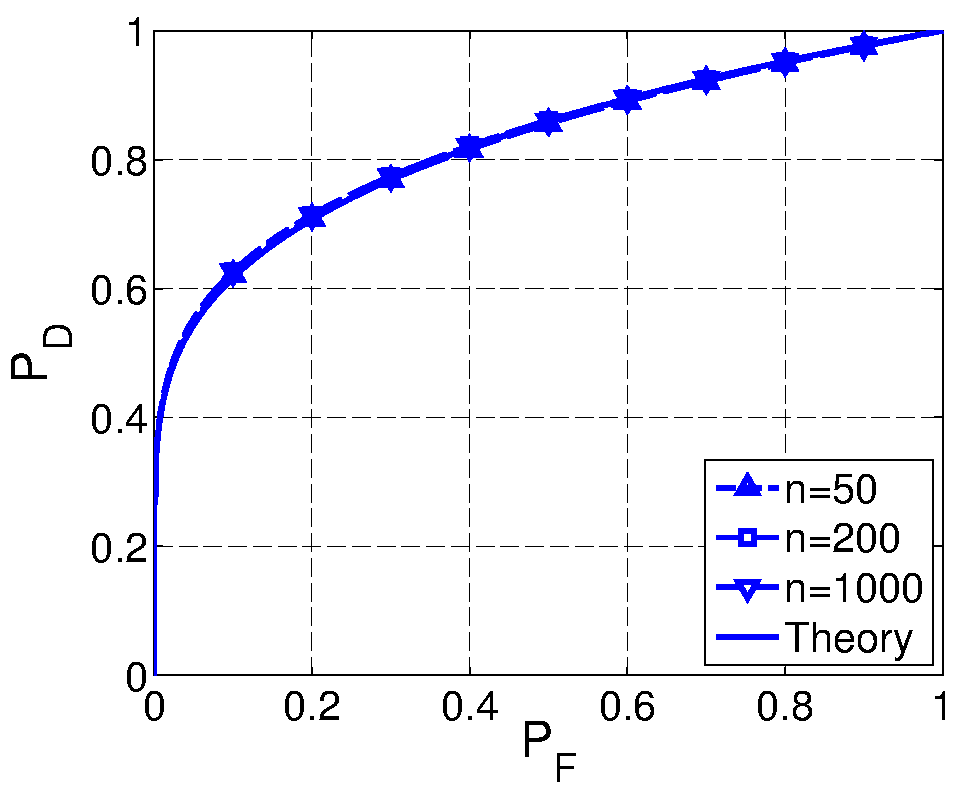
\includegraphics[width=1.5in]{figures/stoch_n_effect1.pdf}
\label{fig:stoch_n_effect1}
}
%\subfigure[$k=2$, $c=10$]{
%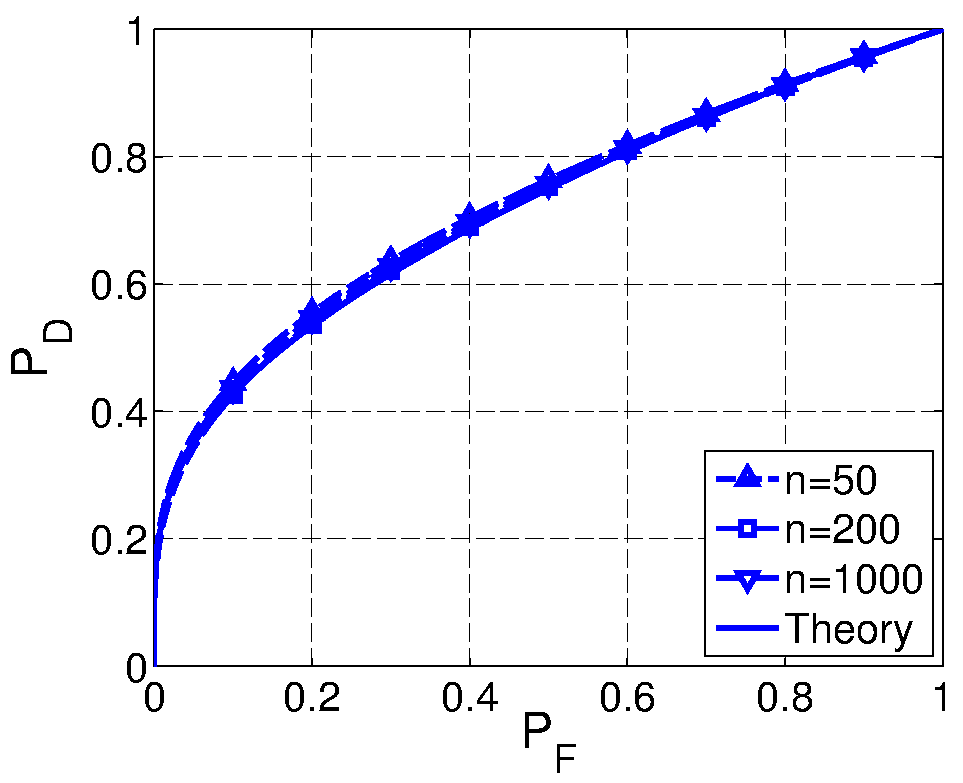
\includegraphics[width=3in]{figures/stoch_n_effect2.pdf}
%\label{fig:stoch_n_effect2}
%}
%\subfigure[$k=4$, $c=1$]{
%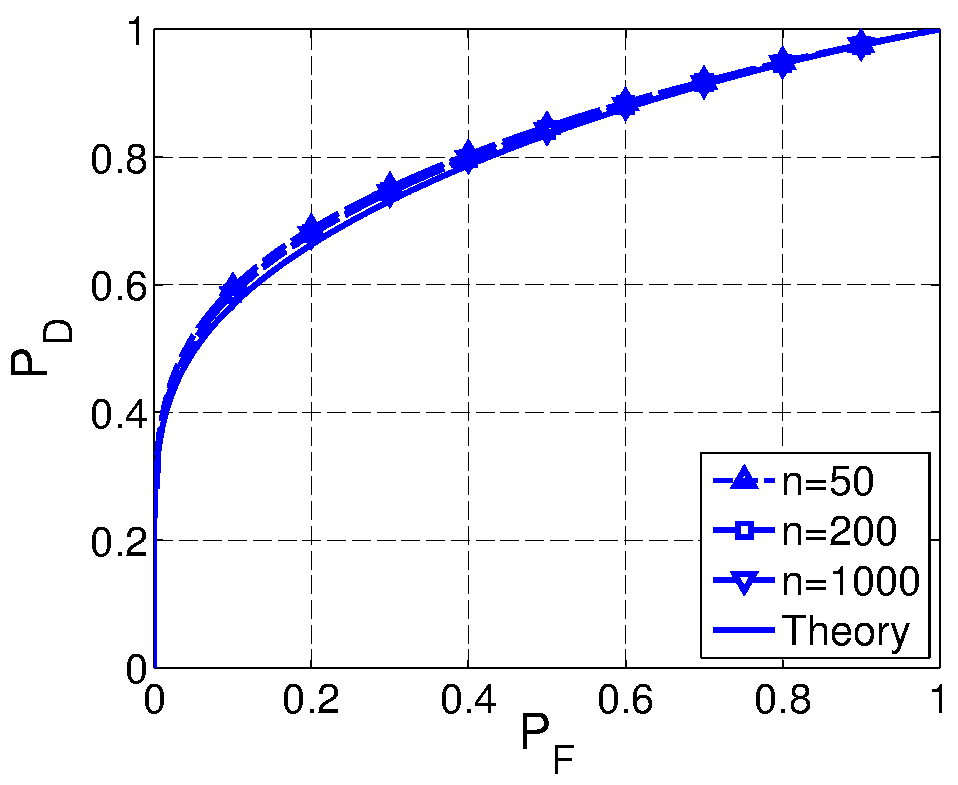
\includegraphics[width=3in]{figures/stoch_n_effect3.pdf}
%\label{fig:stoch_n_effect3}
%}
\subfigure[$k=4$, $c=10$]{
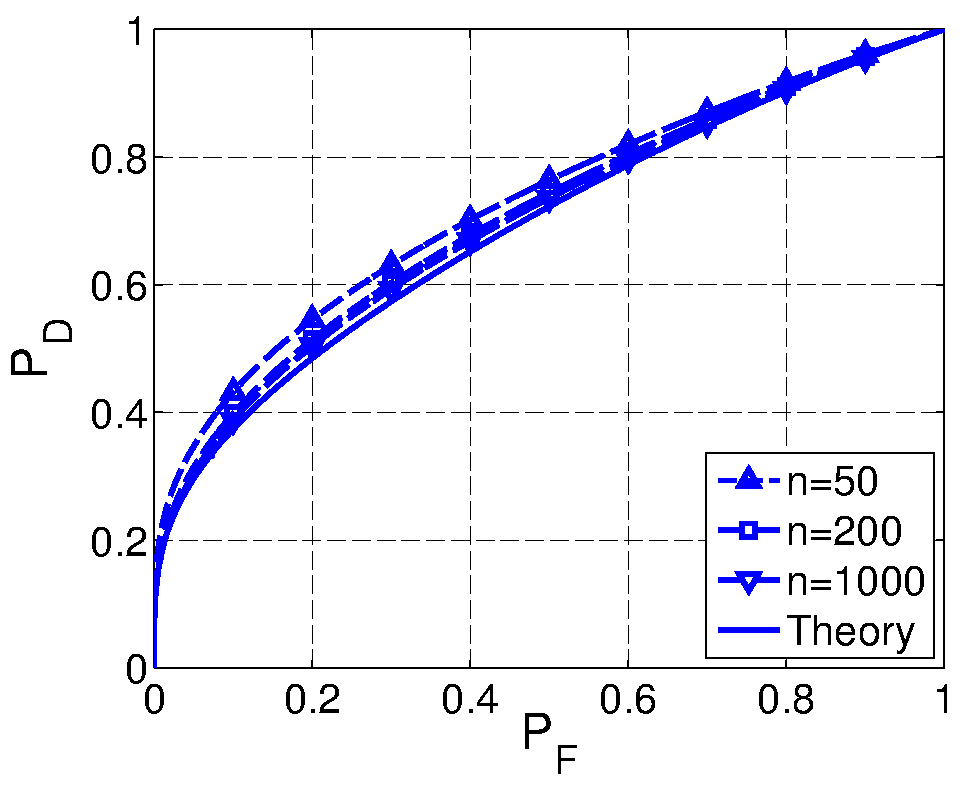
\includegraphics[width=1.5in]{figures/stoch_n_effect4.pdf}
\label{fig:stoch_n_effect4}
}
\vspace{-0.1in}
\caption{Empirical and theoretical ROC curves for the stochastic plug-in detector. Empirical ROC curves were simulated using $10000$ test samples and averaged over 50 trials using algorithms 2 and 4 of \cite{fawcett2006introduction}. (a) $\Sigma=\diag(10,2)$, $c=1$, $\widehat{k}=k=2$ so that $\keff=2$. (b) $\Sigma=\diag(10,2,0.5,0.1)$, $c=10$, $\widehat{k}=k=4$ so that $\keff=1$. Each figure plots empirical ROC curves for $n=50,200,1000$. Theoretical ROC curves were computed as described in Section \ref{sec:roc_theory}. As $n$ increases, the empirical ROC curves approach the theoretically predicted one. However, this convergence is slower for larger $k$ and $c$.}
\vspace{-0.3in}
\end{figure}

\textcolor{blue}{The theoretical ROC curve predictions for the plug-in and RMT detectors rely on the asymptotic approximations that ignore finite $n$ and $m$ correction terms. To examine the validity of the asymptotic approximations (Propositions \ref{th:angles} and \ref{th:eigvals_rmt}, Theorem \ref{th:other angles}, and Corollary \ref{corr:matrix}) and the rate of convergence, we consider two different settings for the stochastic plug-in detector. Figures \ref{fig:stoch_n_effect1}-\ref{fig:stoch_n_effect4} plot three empirical ROC curves for $n=50,200,1000$ as well as the theoretically predicted plug-in ROC curve. Each figure uses different values of $k$ and $c$ but in each case, $\widehat{k}=k$.}

\textcolor{blue}{For both figures, as $n$ increases, the empirical ROC curves approach the theoretical prediction, attesting to the asymptotic convergence of the RMT approximations. Analyzing the rate of convergence (which we conjecture to be $n^{1/2}$ for fixed $k$ and $c$) is an important open problem that we shall tackle in future work. As evident in Figures \ref{fig:stoch_n_effect1}-\ref{fig:stoch_n_effect4} the values of $k$ and $c$ play an important roll in the convergence of the empirical ROC curves. For the larger value of $k$ and $c$ (corresponding to the sample starved regime where the amount of training data is smaller than the system dimensionality i.e. $n>m$) the convergence is also slower. We see that for larger $k$ and $c$, when $n$ is small the empirical ROC curve is not well approximated by the asymptotic theoretical predictions. However, as $n$ increases, the deviation of the empircally generated ROC curve from the theoretically predicted one decreases. Claim \ref{th:other angles} suggests that the off diagonal terms of $\widehat{U}^HU$ asymptotically tend to zero. However, in the finite $n$ and $m$ case these terms are $O(1/\sqrt{n})$ and thus not identically zero. For larger rank systems (increased $k$), there are more of these non-identically-zero terms that worsen the approximation quality for fixed, relatively small $n$. As $n$ increases, this bias vanishes.}

\begin{figure}
\centering
\subfigure[Stochastic]{
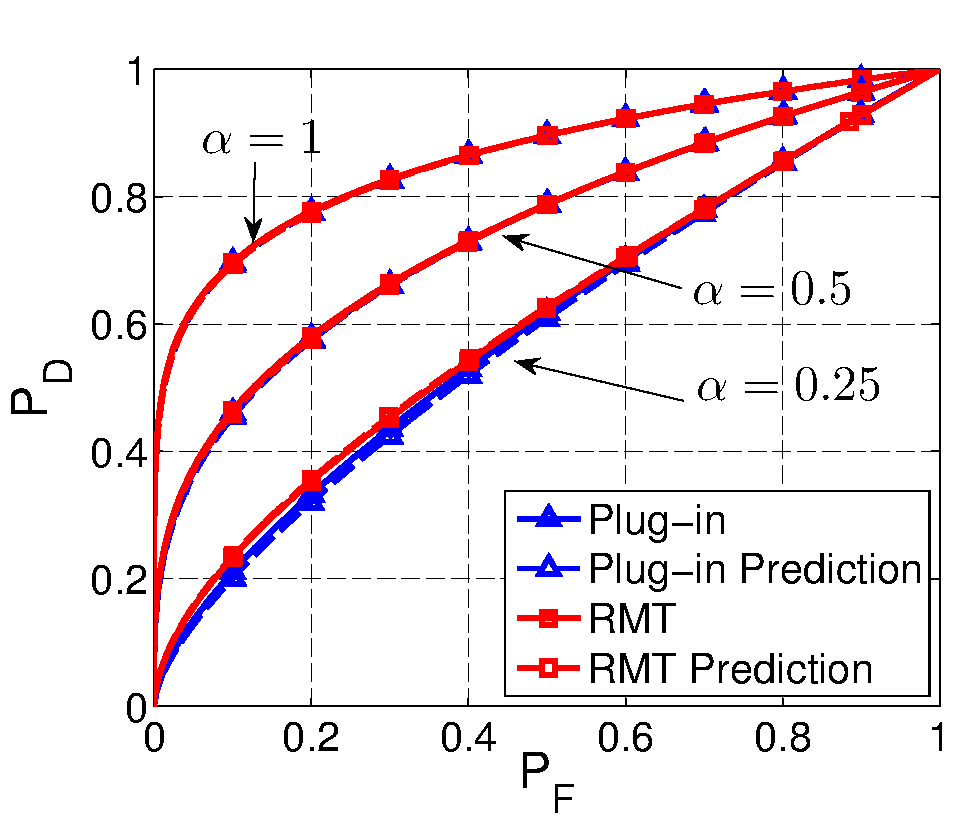
\includegraphics[width=1.5in]{figures/stoch_roc_pred.pdf}
\label{fig:stoch_roc_pred}
}
\subfigure[Deterministic]{
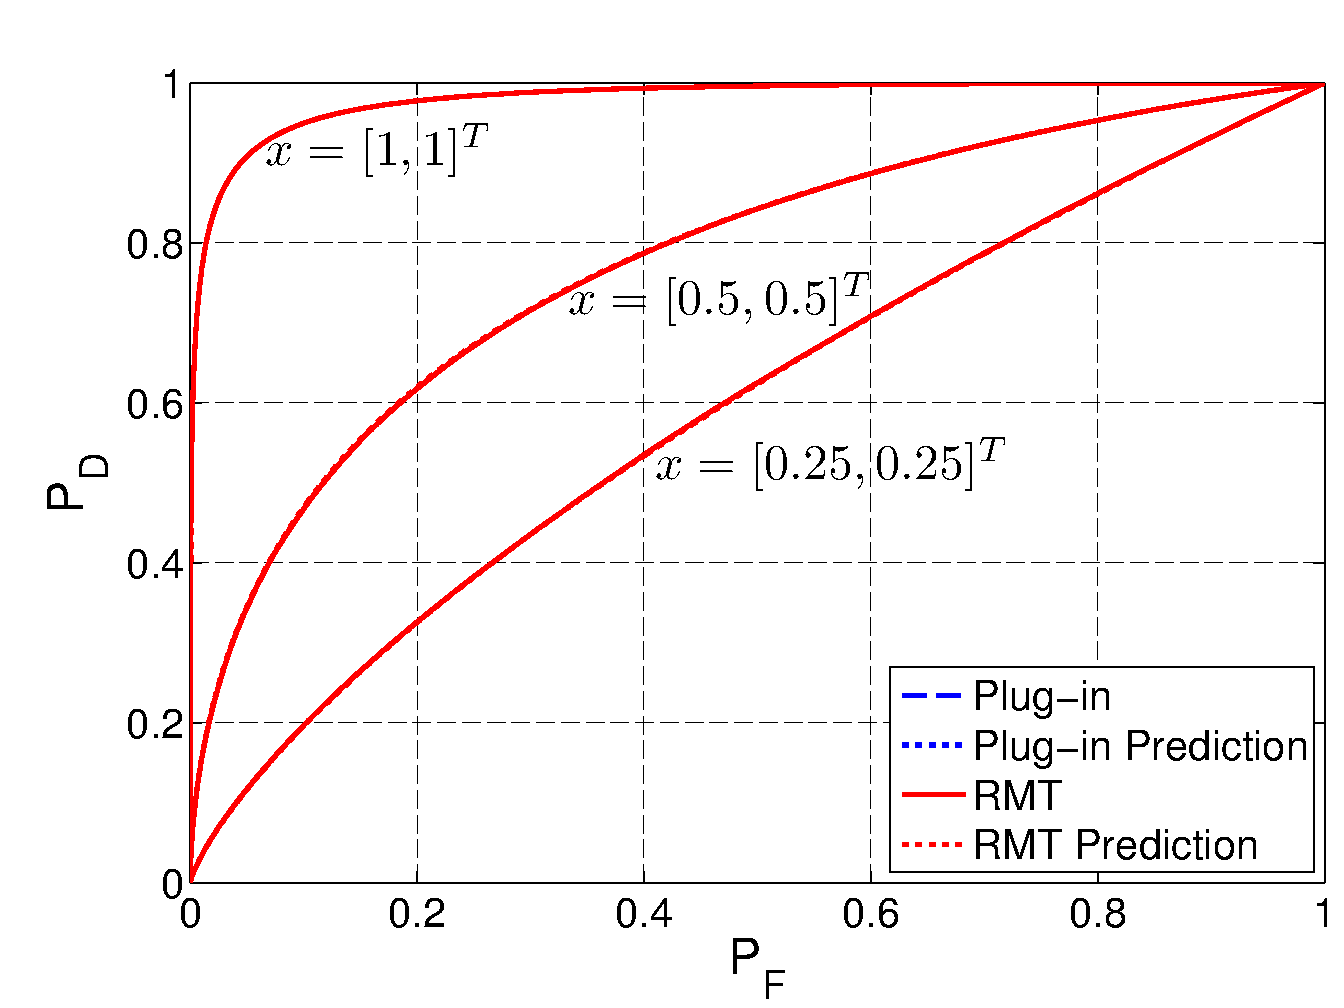
\includegraphics[width=1.5in]{figures/determ_roc_pred.pdf}
\label{fig:determ_roc_pred}
}
\vspace{-0.1in}
\caption{Empirical and theoretical ROC curves for the plug-in and RMT detectors. Empirical ROC curves were simulated using $10000$ test vectors and averaged over 100 trials with $n=1000$, $m=500$, and $\Sigma =\alpha\diag\left(10,5\right)$. The theoretical ROC curves were computed as described in Section \ref{sec:roc_theory}. (a) Stochastic testing seting. Results are plotted for $\alpha=1,0.5,0.25$. For $\alpha=1$ and $\alpha=0.5$, $\widehat{k}=k=k_\text{eff}=2$ by (\ref{eq:keff}). For $\alpha=0.25$, $k_\text{eff}=1$.Since $\widehat{k} > k_{\text{eff}}$ when $\alpha=0.25$, we observe a performance gain when using the RMT detector. (b) Deterministic testing setting. Results are plotted for $\alpha=1$ so that $\keff=2$. Three values of the deterministic signal vector were used: $x=[1,1]^T$, $x=[0.5,0.5]^T$, and $x=[0.25,0.25]^T$. The resulting ROC curves depend on the choice of $x$, however, since $\widehat{k} = k_{\text{eff}}$, the plug-in and RMT detector achieve the same performance for all $x$. For both the stochastic and deterministic detectors, the theoretically predicted ROC curves match the emprical ROC curves, reflecting the accuracy of Corollary \ref{corr:matrix} and the Lugannani-Rice formula.}
\vspace{-0.3in}
\end{figure}

The ROC predictions developed in Section \ref{sec:roc_theory} also depend on parameters such as $\Sigma$ and the deterministic vector $x$. To test the accuracy of the ROC predictions with respect to these parameters, we consider a setting where $\widehat{k}=k = 2$. Figure \ref{fig:stoch_roc_pred} plots empirical and theoretical ROC curves for the plug-in and RMT stochastic detectors for $\Sigma=\alpha\diag(10,5)$ for three choices of $\alpha$. As intuition suggests, smaller values of $\Sigma$ decrease the performance for both the plug-in and RMT detectors. For each choice of $\alpha$, the empirical ROC curves match the ROC predictions that rely on random matrix theoretic approximations presented in Section \ref{sec:rmt}. Using $\alpha=1$ or $\alpha=0.5$ results in $\keff=k=\widehat{k}=2$ but using $\alpha=0.25$ results in $k_\text{eff}=1$. As $\widehat{k}>k_\text{eff}$ for this last case, the plug-in detector realizes a performance loss compared to the RMT detector.

In the deterministic setting, $x$ is an additional parameter that affects detector performance. Figure \ref{fig:determ_roc_pred} plots empirical and theoretical ROC curves for the plug-in and RMT deterministic detectors for $\Sigma=\diag(10,5)$ for three choices of the deterministic test vector $x$. Larger values of $|x|$ result in better detector performance but for each choice of $x$, the theoretically predicted ROC curves match their empirical counterparts. As $x$ does not affect the value of $k_\text{eff}=\widehat{k}=k=2$, the plug-in and RMT detectors achieve the same performance because they have identical statistics. For both test vector models, the theoretical ROC curves match the empirical ROC curves thereby validating the accuracy of the random matrix theoretic approximations employed and the accuracy of the saddlepoint approximation to the c.d.f. used in the stochastic derivation. 

\subsection{Effect of the Number of Training Samples}

\begin{figure}
\centering
\subfigure[$m=5000$]{
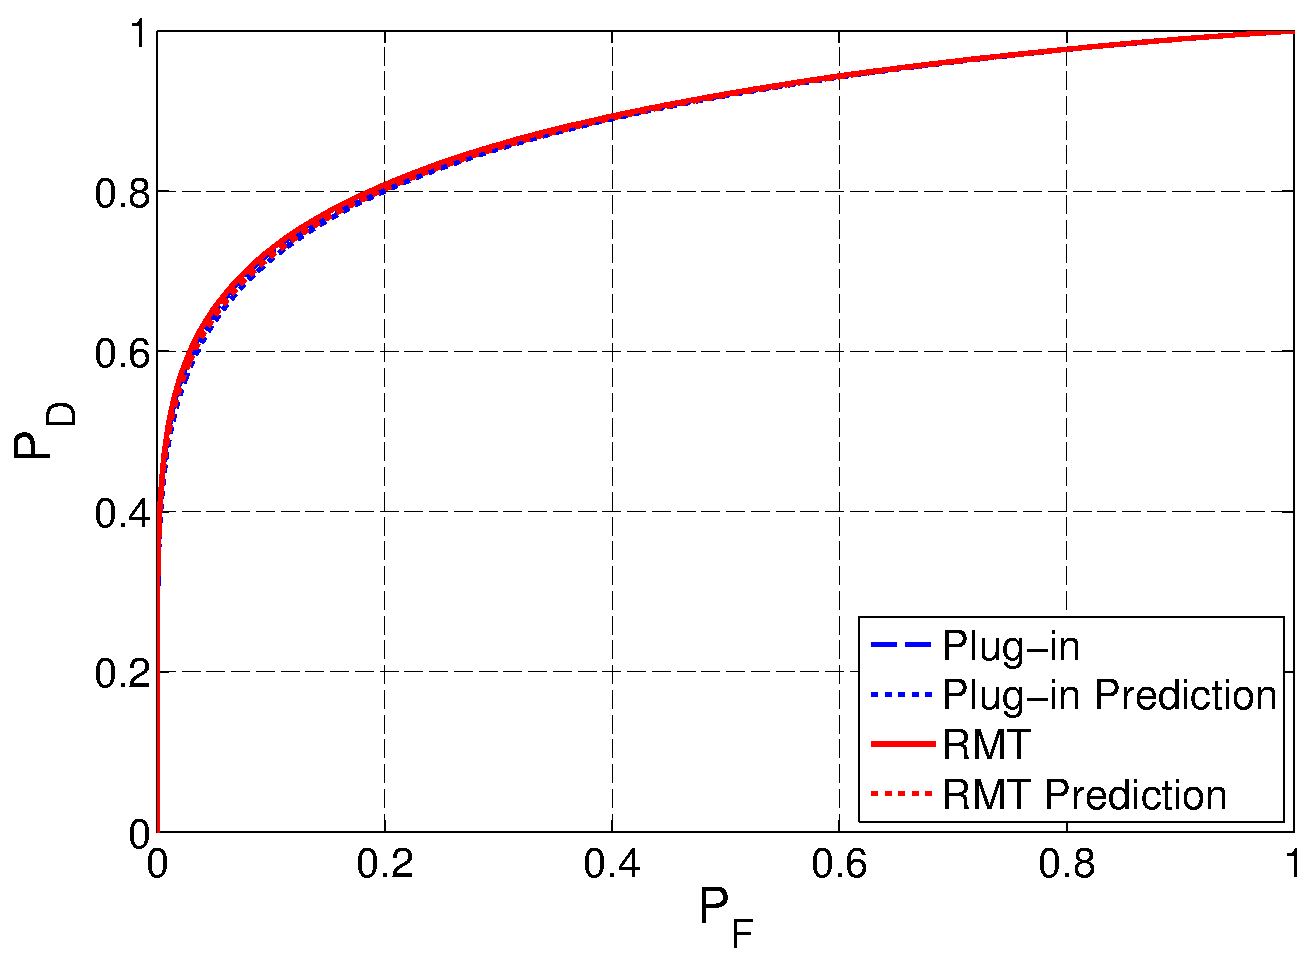
\includegraphics[width=1.5in]{figures/stoch_m_large.pdf}
\label{fig:stoch_m_large}
}
\subfigure[$m=250$]{
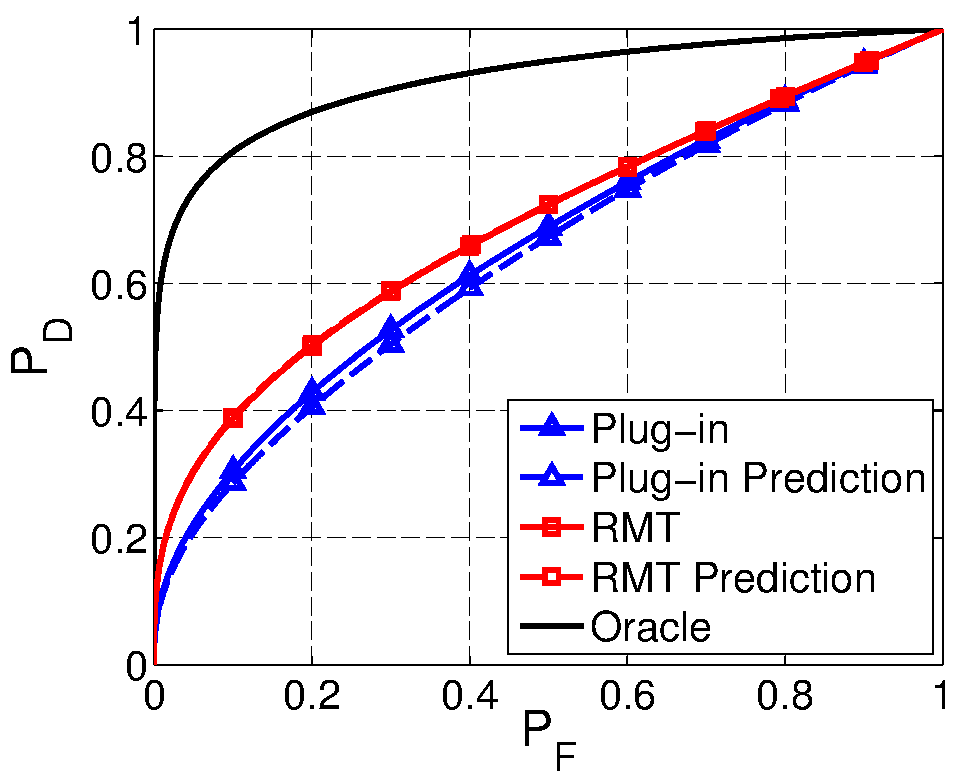
\includegraphics[width=1.5in]{figures/stoch_m_small.pdf}
\label{fig:stoch_m_small}
}
\vspace{-0.1in}
\caption{Empirical and theoretical ROC curves for the plug-in and RMT stochastic detectors. Empirical ROC curves were computed with 10000 test samples and averaged over 100 trials. Here, $n=5000$, $\widehat{k}=k=4$ and $\Sigma = \diag({\bf{10,3,2.5,2}})$. The empirical oracle ROC curve is provided for relative comparison purposes. (a) $m=5000$ so that $c=1$ and $k_\text{eff}=\widehat{k}=4$. The plug-in and RMT detectors achieve relatively the same performance. (b) $m=250$ so that $c=20$ and $\keff=1<\widehat{k}=4$. The RMT detector avoids some of the performance loss realized by the plug-in detector. As seen in Section \ref{sec:std_detecs}, limited training samples degrades detector performance. However, the new RMT detector does not suffer as badly as the plug-in detector because it accounts for subspace estimation errors due to finite training data. The disagreement between the theoretical and empirical ROC curves is attributed to finite dimensionality.}
\label{fig:stoch_m_effect}
\vspace{-0.3in}
\end{figure}

\textcolor{blue}{We saw in Section \ref{sec:training_effect} that finite training data degraded the performance of the plug-in detector relative to that of the oracle detector. The analysis of Section \ref{sec:rmt} mathematically justifies this observation showing that, for a fixed $\Sigma$, the number of training samples, $m$, directly affects $k_\text{eff}$ via (\ref{eq:keff}). While the plug-in detector ignores this analysis, we derived a new RMT detector that accounts for subspace estimation errors due to finite training data. By only using the $\keff$ informative signal subspace components, we hope that the RMT detector will avoid some of the performance loss associated with the plug-in detector. To explore how the number of training samples affects the relative performances of the plug-in and RMT detectors, we first consider the setting where $\widehat{k}=k=4$ with $\Sigma=\diag(10,3,2.5,2)$. }

Figures \ref{fig:stoch_m_large} and \ref{fig:determ_m_large} investigate the performance when $m=n$ so that $c=1$ for the stochastic and deterministic settings, respectively. This choice of $m$ results in $k_\text{eff}=\widehat{k}=4$. As expected, for both settings the plug-in and RMT detectors achieve relatively the same performance because $\widehat{k}=\keff$. Figures \ref{fig:stoch_m_small} and \ref{fig:determ_m_small} choose $20m=n$ so that $c=20$ and $k_\text{eff}=1$ for the stochastic and deterministic settings, respectively. This corresponds to the sample starved regime where $m<n$. In this second experiment, the plug-in detectors becomes suboptimal for both testing settings because they use $4=\widehat{k} > k_\text{eff}=1$ subspace components. Whenever $k_\text{eff}<\widehat{k}$ the RMT detectors avoid some of the performance loss (compared to the oracle detectors) realized by the plug-in detectors. We could have observed this same effect by instead varying $\Sigma$ as both of these quantities drive the value of $k_\text{eff}$. The disagreement between the theoretical and empirical stochastic ROC curves for the plug-in detector is attributed to the finite $n$ and $m$ correction terms, which we have discussed previously.

\textcolor{blue}{Figures \ref{fig:stoch_m_effect} and \ref{fig:determ_m_effect} show that the number of training samples helps to drive the performance of matched subspace detectors. In Section \ref{sec:std_detecs}, we mathematically defined the performance loss of a detector relative to its oracle detector as $\epsilon$ in (\ref{eq:epsilon}) and empirically plotted the number of training samples needed to achieve a desired performance loss for the stochastic plug-in detector in Figure \ref{fig:epsilon_graph}. Figures \ref{fig:stoch_theory_epsilon} and \ref{fig:determ_theory_epsilon} theoretically plot this same curve for the plug-in and RMT detectors for each testing setting, respectively.}

\textcolor{blue}{These figures show that when $\keff<\widehat{k}$, the RMT detector achieves a much smaller performance loss for a fixed number of training samples. Put another way, to achieve the same performance loss, the RMT detectors need a significantly less number of training samples when $\keff<\widehat{k}$. Figure \ref{fig:stoch_theory_epsilon} shows that the stochastic detectors can acheive an arbitrarily small performance loss given a particularly large number of training samples. However, Figure \ref{fig:determ_theory_epsilon} shows that there is a performance loss limit for the deterministic detectors and that this limit may be different for the RMT and plug-in detectors. As discussed in Section \ref{sec:std_detecs}, this arises because the oracle deterministic detector assumes that $x$ is known. As $m\to\infty$, $\widehat{U}\to U$ and $\widehat{\Sigma}\to\Sigma$, however, the plug-in detector's estimate of $\widehat{x}$ still depends on the noisy observed data $y$. Therefore, unlike the stochastic detectors that can achieve an arbitrarily small performance loss, the deterministic plug-in and RMT detectors can never achieve the same performance as the deterministic oracle detector.}

\begin{figure}
\centering
\subfigure[$m=5000$]{
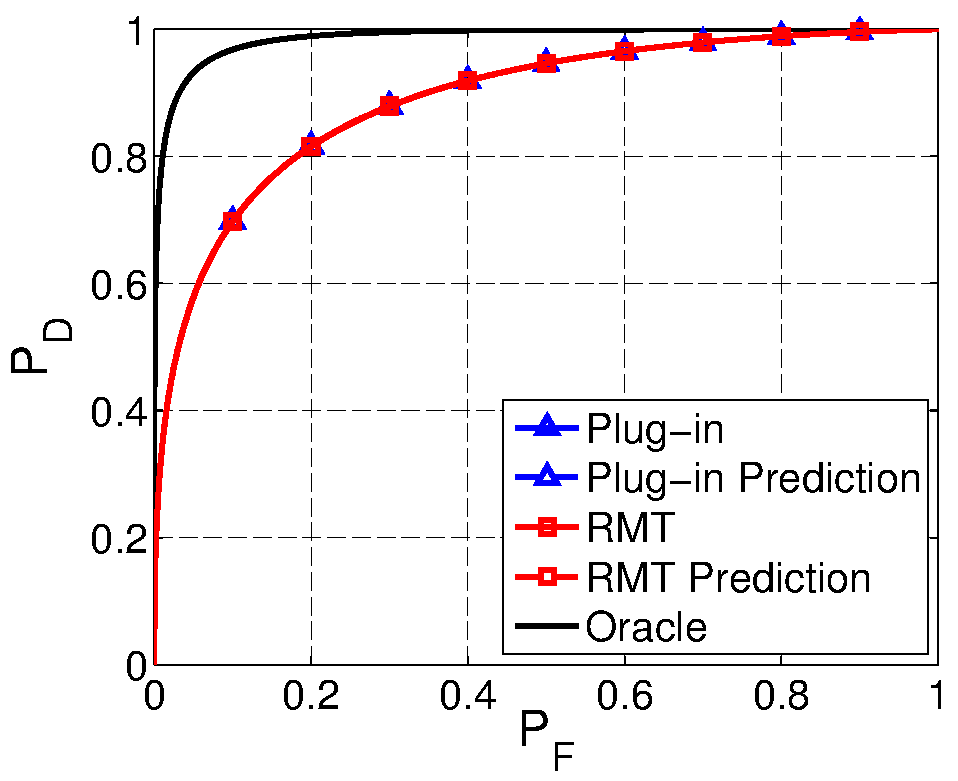
\includegraphics[width=1.5in]{figures/determ_m_large.pdf}
\label{fig:determ_m_large}
}
\subfigure[$m=250$]{
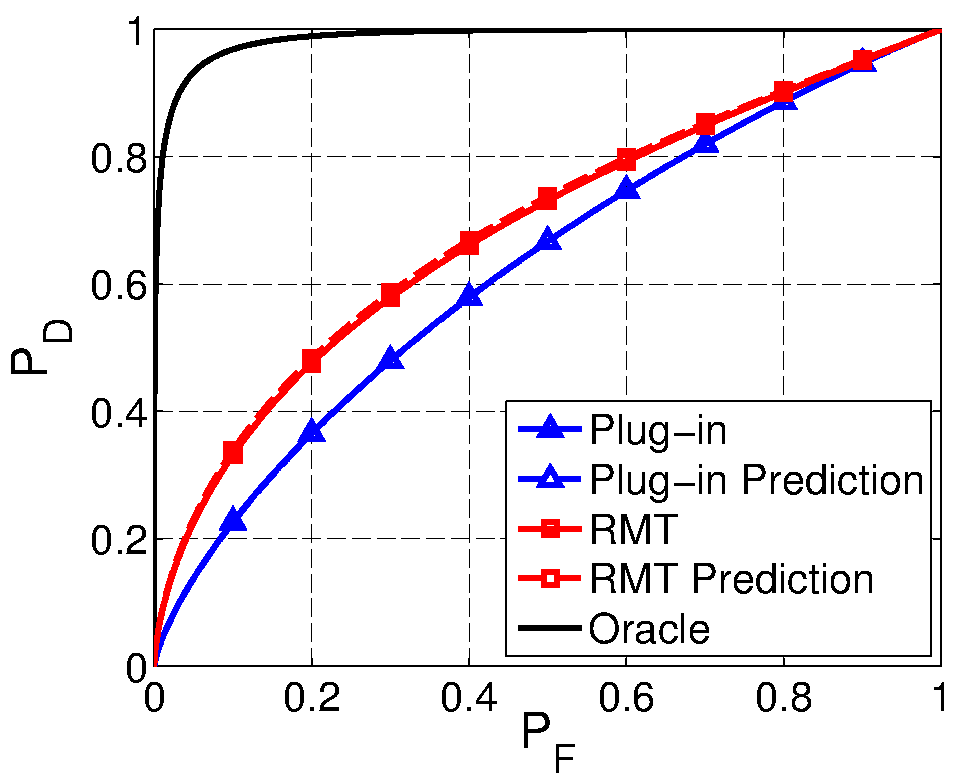
\includegraphics[width=1.5in]{figures/determ_m_small.pdf}
\label{fig:determ_m_small}
}
\vspace{-0.1in}
\caption{Analagous figures to Figures \ref{fig:stoch_m_large} and \ref{fig:stoch_m_small} for the deterministic detectors when $x=0.75\times[1,1,1,1]^T$. When $\keff<\widehat{k}$ we see that the RMT detector avoids some of the performance loss of the plug-in detector due to finite training data.}
\label{fig:determ_m_effect}
\vspace{-0.2in}
\end{figure}

\begin{figure}
\centering
\subfigure[Stochastic]{
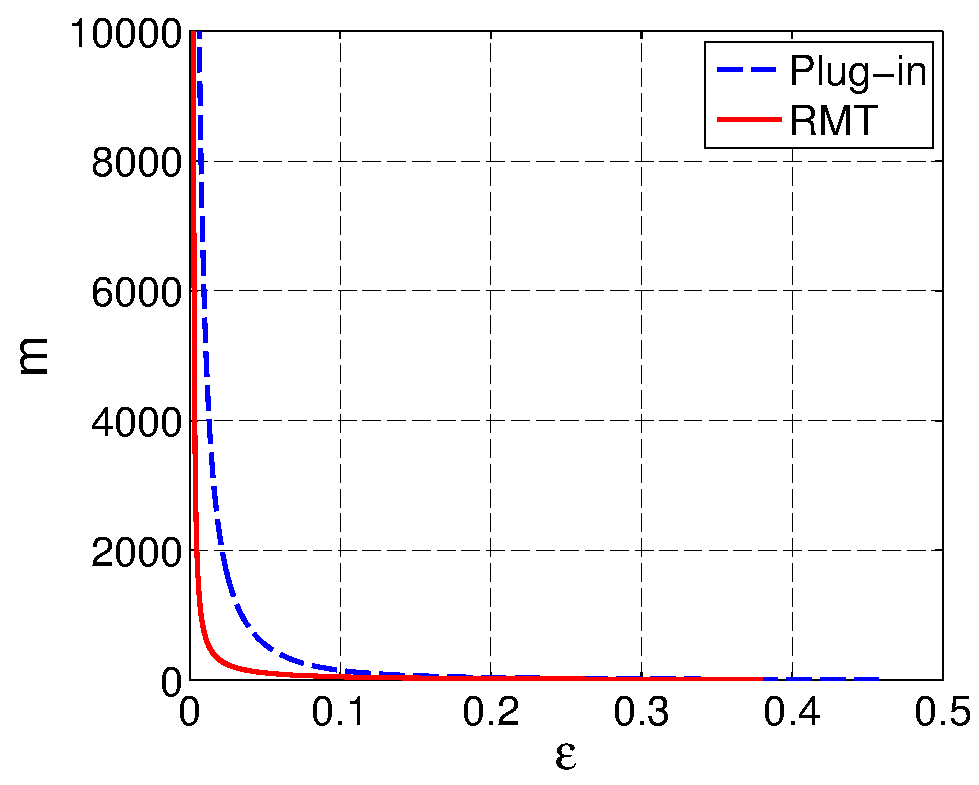
\includegraphics[width=1.5in]{figures/stoch_theory_epsilon_graph.pdf}
\label{fig:stoch_theory_epsilon}
}
\subfigure[Deterministic]{
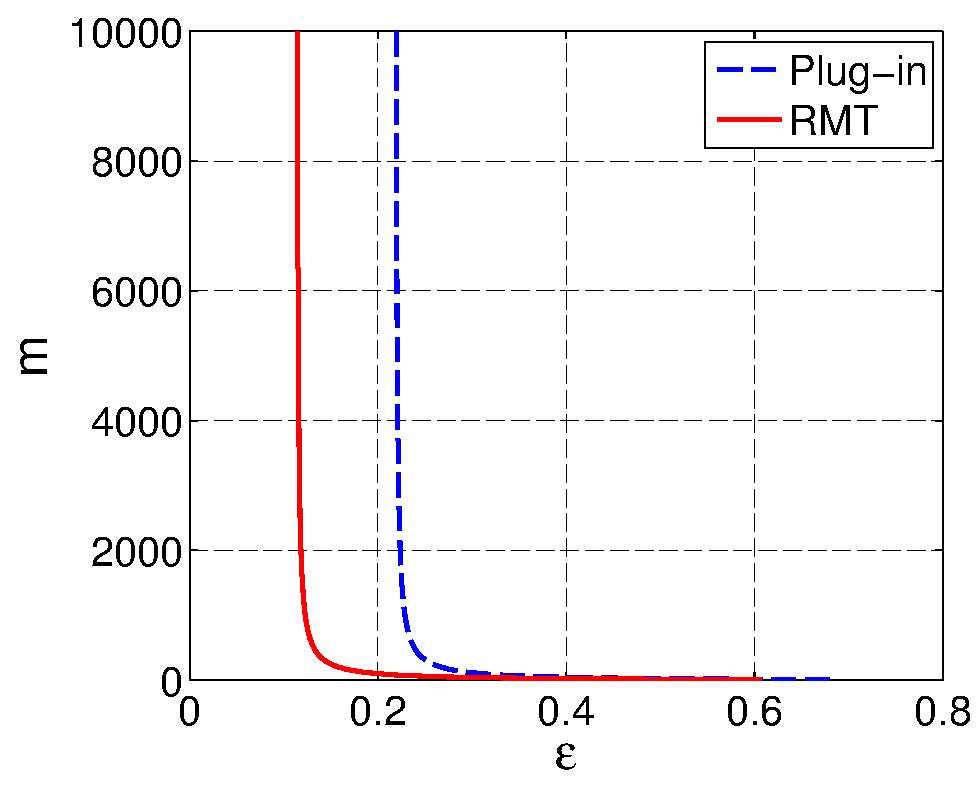
\includegraphics[width=1.5in]{figures/determ_theory_epsilon_graph.pdf}
\label{fig:determ_theory_epsilon}
}
\vspace{-0.1in}
\caption{Theoretically determined number of training samples, $m$, needed to achieve a desired performance loss, $\epsilon$, as defined in (\ref{eq:epsilon}). The required false alarm rate is $P_F=0.1$ with $n=200$, $\Sigma = \diag(10,0.1)$, and $\widehat{k}=k=2$. (a) Results for the stochastic detectors. We see that for a given $\epsilon$, the new RMT detector requires less training samples. (b) Results for the deterministic detectors when $x=[0.75,0.75]^T$. Again, for a given $\epsilon$, the new RMT detector requires less training samples. In the deterministic setting, the limiting performance loss is different (and non-zero) for the plug-in and RMT detectors. This arises in estimation errors of $x$ in the GLRT.}
\label{fig:epsilon_combined}
\end{figure}


%we have neglected. As $k$ increases, there are more off-diagonal terms in the covariance matrix in (\ref{eq:cov mat}) that are not identically zero, as discussed earlier. Theorem \ref{th:other angles} shows that asymptotically these off diagonal terms decay to zero but in the finite $n$ and $m$ case, they are non-zero. In the case of larger $k$, there are more of these non-identically-zero terms thereby worsening the approximation.

\subsection{Effect of $\widehat{k}$}
\begin{figure}
\centering
\subfigure[Stochastic]{
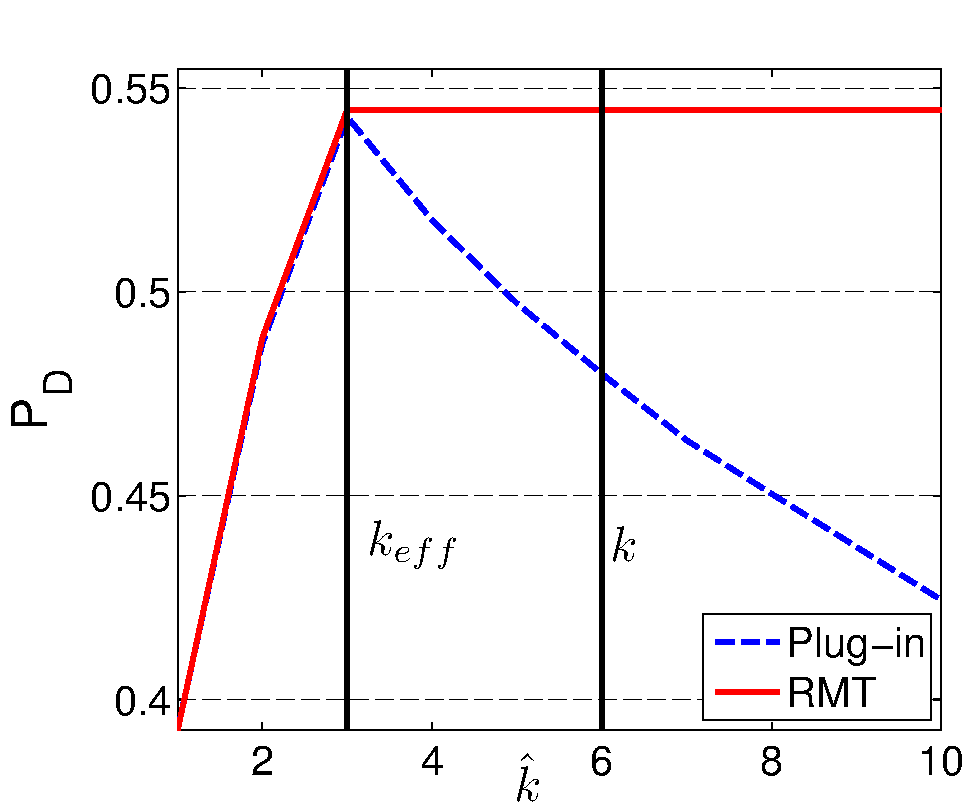
\includegraphics[width=1.5in]{figures/stoch_khat_graph.pdf}
\label{fig:stoch_khat}
}
\subfigure[Deterministic]{
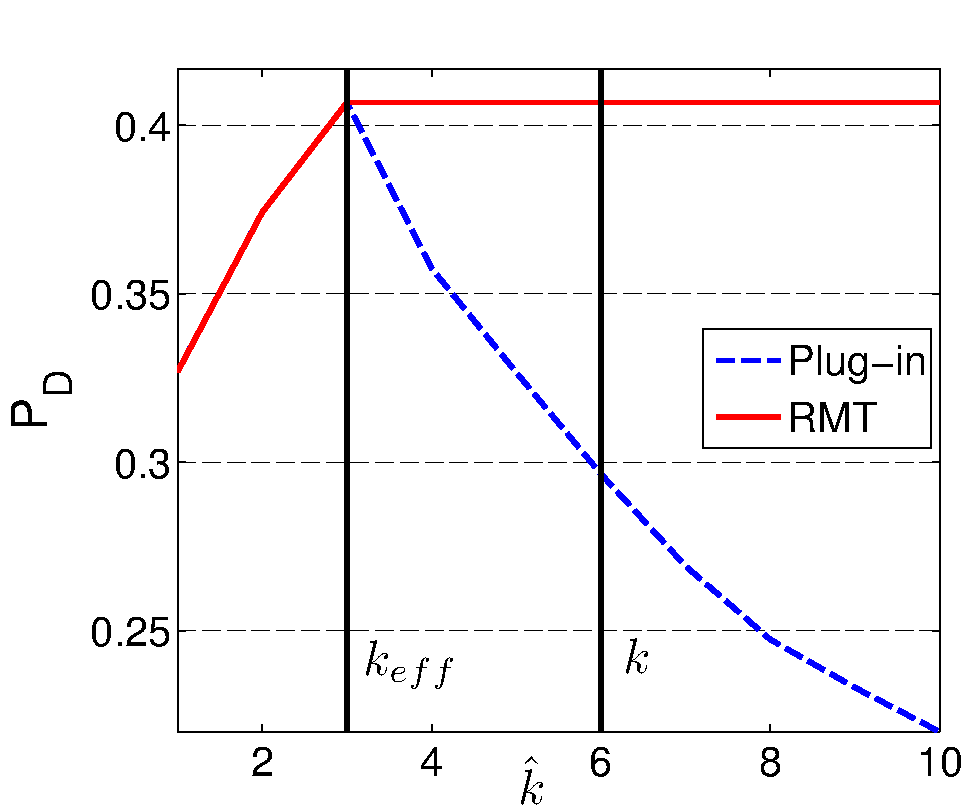
\includegraphics[width=1.5in]{figures/determ_khat_graph.pdf}
\label{fig:determ_khat}
}
\vspace{-0.1in}
\caption{Empirical exploration of the achieved probability of detection, $P_D$, for a fixed probability of false alarm, $P_F=0.01$, for various $\widehat{k}$. Empirical ROC curves were computed using 10000 test samples and averaged over 100 trials with $n=1000$, $m=500$, and $\Sigma = \diag({\bf{10,5,4}},0.75,0.5,0.25)$ so that $k_{\text{eff}}=3$. (a) Results for the stochastic detectors. (b) Results for the deterministic detecotrs using $x=0.75\times[1,1,1,1,1,1]^T$. In both test settings, the optimal $\widehat{k}$ resulting in the largest $P_D$ is not the true $k$, but rather $k_\text{eff}$.}
\label{fig:khat_graphs}
\vspace{-0.3in}
\end{figure}

\textcolor{blue}{We discussed in Section \ref{sec:param_estim} that we are given a dimension estimate $\widehat{k}$ when deriving our detector. From our perspective, we don't know how $\widehat{k}$ was estimated (possibly from the training data or by a domain expert) but simply use it when forming our subpsace and signal covariance estimates.} Figures \ref{fig:stoch_khat} and \ref{fig:determ_khat} empirically examine the performance of the plug-in and RMT detectors as a function of $\widehat{k}$ for the stochastic and deterministic test settings, respectively. Here, we relax the constraint that $\widehat{k}\geq k$. The figures plot the achieved probability of detection for a constant false alarm rate of $0.01$. The result confirms that, for both settings, $k_\text{eff}$ is the optimal choice for $\widehat{k}$. When the plug-in detectors use $\widehat{k} = k_\text{eff}$ they achieve an equivalent performance as that of the RMT detector.

Setting $\widehat{k} < \keff$ drastically degrades performance for all detectors. In this regime, the plug-in and RMT detectors realize the same ROC performance, demonstrating that quantification and exploitation of the subspace estimation accuracy ($|\langle u_i,\widehat{u}_i\rangle |^2_{\text{rmt}}$ and $\sigma_{i_\text{rmt}}^2$), while useful in ROC performance prediction, does \textit{not} noticeably enhance detection performance. When $\widehat{k} > k_\text{eff}$, the performances of the plug-in detectors degrade while those of the RMT detectors are stable as if $\widehat{k}=k_\text{eff}$. In other words, we do not pay a price for overestimating the subspace dimension with the RMT detectors. This makes sense (and is slightly contrived) because the RMT detectors will only sum to a maximum of $k_\text{eff}$ indices as evident in (\ref{eq:optimal_stat_stoch}) and (\ref{eq:optimal_stat_determ}). In many applications, practitioners might employ the ``play-it-safe'' approach and set $\widehat{k}$ to be significantly greater than $k_\text{eff}$. The performance loss caused by adding each uninformative subspace, as seen in Figure \ref{fig:khat_graphs}, constitutes evidence to the assertion that overestimating the signal subspace dimension is a bad idea. When $k_\text{eff} < k$, even perfectly estimating the subspace dimension (i.e. setting $\widehat{k} = k$) is suboptimal.


\section{Conclusion}\label{sec:conclusion}
In this paper, we considered a matched subspace detection problem where the low-rank signal subspace is unknown and must be estimated from finite, noisy, signal-bearing training data. We considered both a stochastic and deterministic model for the testing data. The subspace estimate is inaccurate due to finite and noisy training samples and therefore degrades the performance of plug-in detectors compared to an oracle detector. We showed how the ROC performance curve can be derived from the RMT-aided quantification of the subspace estimation accuracy.

Armed with this RMT knowledge, we derived a new RMT detector that only uses the effective number of informative subspace components, $k_\text{eff}$. Plug-in detectors that use the uninformative components will thus incur a performance degradation, relative to the RMT detector. \textcolor{blue}{In settings where a practitioner might play-it-safe and set $\widehat{k}> \widehat{k}_{\text{eff}}$, the performance loss in significant (see Figures \ref{fig:stoch_theory_epsilon} and \ref{fig:determ_theory_epsilon} for a demonstration of how much training data such a play-it-safe plug-in detector would need to match the performance of a $\keff$-tuned RMT detector).} This highlights the importance of robust techniques \cite{nadakuditi2010fundamental,johnstone2001distribution,el2007tracy} for estimating $k_\text{eff}$ in subspace based detection schemes as opposed to estimating $k$, particularly in the regime where $k_{\text{eff}} < k$.  We showed in Tables \ref{table:summary_stoch} and \ref{table:summary_determ} that the distributions of the test statistics could be expressed as a weighted sum of independent chi-squared random variables. The associated ROC curves can then be computed using a saddlepoint approximation.

\textcolor{blue}{The results in this paper can be extended in several directions. We note that the stochastic detector setting assumed normally distributed training and test data. We can extend the analysis to the Gaussian training data but non-Gaussian test vector setting by `integrating-out' the deterministic detector performance curves with respect to the non-Gaussian distribution of the test-vector. Our results relied on characterization of the quantity $\langle u_{j},\widehat{u}_{i}\rangle$.  Thus analogous performance curves can be obtained for any alternate training data models for which this quantity can be analytically quantified. To that end, the results in \cite{benaych2011singular} facilitate such an analysis for a broader class of models including the correlatted Gaussians training data setting. An extension to the missing data setting might follow a similar approach and appears within reach. Aspects related to rate of convergence are open and will be the subject of future work.}



\section*{Appendix}
\textit{Theorem 5.1:} Assume the same hypothesis as in Proposition \ref{th:angles}. Let $\widehat{k}=\keff=k$. For $i=1,\dots,\widehat{k}$, $j=1,\dots,k$, and $i\neq j$, as $n,m\to\infty$ with $n/m\to c$, then $\langle u_j,\widehat{u}_i\rangle \convas 0.$
\begin{proof}
Let $U_{n,k}$ be a $n\times k$ real or complex matrix with orthonormal columns, $u_i$ for $1\leq i\leq k$. Let $\Sigma = \diag\left(\sigma_1^2,\dots,\sigma_k^2\right)$ such that $\sigma_1^2>\sigma_2^2>\dots>\sigma_k^2>0$ for $k\geq 1$. Define $P_n=U_{n,k}\Sigma U_{n,k}^H$ so that $P_n$ is rank-$k$. Let $Z_n$ be a $n\times m$ real or complex matrix with independent $\mathcal{CN}\left(0,1\right)$ entries. Let $X_n=\frac{1}{m}Z_nZ_n^H$, which is a random Wishart matrix, have eigenvalues $\lambda_1(X_n)\geq\dots\geq\lambda_n(X_n)$. Let $\widehat{X}_n=X_n\left(I_n+P_n\right)$. $X_n$ and $P_n$ are independent by assumption. Define the empirical eigenvalue distribution as $\mu_{X_n}=\frac{1}{n}\sum_{j=1}^n\delta_{\lambda_j\left(X_n\right)}$. We assume that as $n\to\infty$, $\mu_{X_n}\overset{\text{a.s.}}{\longrightarrow}\mu_X$.


For $i=1,\dots, \widehat{k}=k$, let $\widehat{v}_i$ be an arbitrary unit eigenvector of $\widehat{X}_n$. By the eigenvalue master equation, $\widehat{X}_n\widehat{v}_i=\widehat{\lambda}_i\widehat{v}_i$, it follows that
\begin{equation}\label{eq:eval_master}
\begin{aligned}
  &U_{n,k}^H\left(\widehat{\lambda}_iI_n-X_n\right)^{-1}X_nU_{n,k}\Sigma U_{n,k}^H\widehat{v}_i&&=U_{n,k}^H\widehat{v}_i.\\
\end{aligned}
\end{equation}
Let $X_n=V_n\Lambda_nV_n^H$ be the eigenvalue decomposition of $X_n$ such that $\Lambda_n=\diag(\lambda_1(X_n),\dots,\lambda_n(X_n))$ and $\lambda_1(X_n)\geq\dots\geq\lambda_n(X_n)$. Using this decomposition and defining $W_{n,k}=V^HU_{n,k}$, (\ref{eq:eval_master}) simplifies to
\begin{equation}\label{eq:eval_master2}
\begin{aligned}
  &W_{n,k}^H\left(\widehat{\lambda}_iI_n-\Lambda_n\right)^{-1}\Lambda_nW_{n,k}\Sigma U_{n,k}^H\widehat{v}_i&&=U_{n,k}^H\widehat{v}_i.\\
\end{aligned}
\end{equation}
Define the columns of $W_{n,k}$ to be $w_j^{(n)}=[w_{1,j}^{(n)},\dots,w_{n,j}^{(n)}]^T$ for $j=1,\dots,k$. These columns are orthonormal and isotropically random. We can rewrite (\ref{eq:eval_master2}) as
\begin{equation}\label{eq:t_trans}
\left[T_{\mu_{r,j}^{\left(n\right)}}\left(\widehat{\lambda}_i\right)\right]_{r,j=1}^k \Sigma U_{n,k}^H\widehat{v}_i=U_{n,k}^H\widehat{v}_i
\end{equation}
where for $r=1,\dots,k$, $j=1,\dots,k$, $\mu_{r,j}^{\left(n\right)}=\sum_{\ell=1}^n\overline{w_{\ell,r}^{\left(n\right)}}w_{\ell,j}^{\left(n\right)}\delta_{\lambda_\ell\left(X_n\right)}$ is a complex measure and $T_{\mu_{r,j}^{\left(n\right)}}$ is the T-transform defined by $T_{\mu}\left(z\right) = \int\frac{t}{z-t}d\mu\left(t\right)\,\,\,\,\text{for } z\not\in\text{supp } \mu$. We may rewrite (\ref{eq:t_trans}) as
\begin{equation*}
\left(I_k-\left[\sigma_j^2T_{\mu_{r,j}^{\left(n\right)}}\left(\widehat{\lambda}_i\right)\right]_{r,j=1}^k\right)U_{n,k}^H\widehat{v}_i=0.
\end{equation*}
Therefore, $U_{n,k}^H\widehat{v}_i$ must be in the kernel of $M_n\left(\widehat{\lambda}_i\right)=I_k-\left[\sigma_j^2T_{\mu_{r,j}^{\left(n\right)}}\left(\widehat{\lambda}_i\right)\right]_{r,j=1}^k$.
By Proposition 9.3 of \cite{benaych2011eigenvalues}
\begin{equation*}
\mu_{r,j}^{\left(n\right)}\overset{\text{a.s.}}{\longrightarrow}\begin{cases}\mu_X & \text{for } i=j \\ \delta_0 & \text{o.w.} \end{cases}
\end{equation*}
where $\mu_X$ is the limiting eigenvalue distribution of $X_n$. Therefore,
\begin{equation*}
M_n\left(\widehat{\lambda}_i\right)\overset{\text{a.s.}}{\longrightarrow}\diag\left(1-\sigma_1^2T_{\mu_X}\left(\widehat{\lambda}_i\right), \dots, 1-\sigma_k^2T_{\mu_X}\left(\widehat{\lambda}_i\right)\right).
\end{equation*}
As $k_\text{eff}=k$, for $i=1,\dots,k$, $\sigma_i^2>1/T_{\mu_X}(b^+)$, where $b$ is the supremum of the support of $\mu_X$. As $\widehat{\lambda}_i$ is the eigenvalue corresponding to the eigenvector $\widehat{v}_i$, by Theorem 2.6 of \cite{benaych2011eigenvalues} $\widehat{\lambda}_i\overset{\text{a.s.}}{\longrightarrow}T^{-1}_{\mu_X}\left(1/\sigma_i^2\right)$. Therefore,
\footnotesize\begin{equation}\label{eq:Mn}
M_n\left(\widehat{\lambda}_i\right)\overset{\text{a.s.}}{\longrightarrow}\diag\left(1-\frac{\sigma_1^2}{\sigma_i^2}, \dots, 1-\frac{\sigma_{i-1}^2}{\sigma_i^2}, 0, 1-\frac{\sigma_{i+1}^2}{\sigma_i^2}, \dots, 1-\frac{\sigma_k^2}{\sigma_i^2}\right)
\end{equation}\normalsize
Recall that $U_{n,k}^H\widehat{v}_i$ must be in the kernel of $M_n\left(\widehat{\lambda}_i\right)$. Therefore, any limit point of $U_{n,k}^H\widehat{v}_i$ is in the kernel of the matrix on the right hand side of (\ref{eq:Mn}). Therefore, for $i\neq j$, $i=1,\dots,\widehat{k}$, $j=1,\dots,k$, we must have that $\left(1-\frac{\sigma_j^2}{\sigma_i^2}\right)\langle u_j,\widehat{v}_i\rangle=0$. As $\sigma_i^2\neq\sigma_j^2$, for this condition to be satisfied we must have that for $j\neq i$, $i=1,\dots,\widehat{k}$, $j=1,\dots,k$, $\langle u_j,\widehat{v}_i\rangle\overset{\text{a.s.}}{\longrightarrow}0$.

Recall that our observed vectors $y_i\in\complex^{n\times 1}$ have covariance matrix $U_{n,k}\Sigma U_{n,k}^H+I_n=P_n+I_n$. Therefore, our observation matrix, $Y_n$ which is a $n\times m$ matrix, may be written $Y_n=\left(P_n+I_n\right)^{1/2}Z_n$. The sample covariance matrix, $S_n=\frac{1}{m}Y_nY_n^H$, may be written $S_n=\left(I_n+P_n\right)^{1/2}X_n\left(I_n+P_n\right)^{1/2}$. By similarity transform, if $\widehat{v}_i$ is a unit-norm eigenvector of $\widehat{X}_n$ then $\widehat{s}_i=\left(I_n+P_n\right)^{1/2}\widehat{v}_i$ is an eigenvector of $S_n$. If $\widehat{u}_i=\widehat{s}_i/\|\widehat{s}_i\|$ is a unit-norm eigenvector of $S_n$, it follows that
\begin{equation*}
\langle u_j,\widehat{u}_i\rangle=\frac{\sqrt{\sigma_i^2+1}\langle u_j,\widehat{v}_i\rangle}{\sqrt{\sigma_i^2|\langle u_j,\widehat{v}_i\rangle|^2+1}}
\end{equation*}
As $\langle u_j,\widehat{v}_i\rangle\overset{\text{a.s.}}{\longrightarrow}0$ for all $i\neq j$, $i=1,\dots,\widehat{k}$, $j=1,\dots,k$, it follows that $\langle u_j,\widehat{u}_i\rangle\overset{\text{a.s.}}{\longrightarrow}0$ for all $i\neq j$ $i=1,\dots,\widehat{k}$, $j=1,\dots,k$.

%%%%%%%%%%%%%%%%%%%%% CLAIM %%%%%%%%%%%%%%%%%%%%%%%%%%%%%%%%%%%%%%%%%%%%%

\textit{Claim 5.1:}  We conjecture that this result holds for the general case of $i\neq
j$, $i=1,\dots,\widehat{k}$, $j=1,\dots,k$, not just when $\widehat{k}=\keff=k$. Consider
the case when $k=1$. For $i>2$, if $\widehat{\lambda}_i$ is an eigenvalue of
$\widehat{X}_n=X_n(I_n+\sigma^2uu^H)$, then it satisfies
$\det(\widehat{\lambda}_iI_n-X_n(I_n+\sigma^2uu^H)) =
\det(\widehat{\lambda}_iI_n-X_n)\det(I_n-(\widehat{\lambda}_iI_n-X_n)^{-1}X_n\sigma^2uu^H)=0$. Therefore,
if $\widehat{\lambda}_i$ is not an eigenvalue of $X_n$, the corresponding unit norm
eigenvector $\widehat{v}_i$ is in the kernel of
$I_n-(\widehat{\lambda}_iI_n-X_n)^{-1}X_n\sigma^2uu^H$. Therefore
\begin{equation*}
  |\langle \widehat{v}_i,u\rangle |^2 = \frac{1}{\sigma^4u^HX_n\left(\widehat{\lambda}_iI_n-X_n\right)^{-2}X_nu}.
\end{equation*}
Recall that Weyl's interlacing lemma for eigenvalues gives $\lambda_i(X_n)\leq
\widehat{\lambda}_i\leq \lambda_{i-1}(X_n)$. Letting $X_n=V_n\Lambda_nV_n^H$ and
$w=V_n^Hu$, we see the importance of the
asymptotic spacing of eigenvalues of $X_n$ in
%\begin{equation*}
%  u^HX_n(\widehat{\lambda}_jI_n-X_n)^{-2}X_nu =\sum_{\ell=1}^n\frac{|w_\ell|^2\lambda_\ell^2(X_n)}{\left(\widehat{\lambda}_j-\lambda_\ell\right)^2}\geq\frac{|w_{j-1}|^2\lambda_{j-1}^2(X_n)}{|\lambda_{j-1}-\lambda_j|^2}+\frac{|w_{j}|^2\lambda_j^2(X_n)}{|\lambda_{j-1}-\lambda_j|^2}.
%\end{equation*}
\begin{equation*}
  u^HX_n(\widehat{\lambda}_iI_n-X_n)^{-2}X_nu
  =\sum_{\ell=1}^n\frac{|w_\ell|^2\lambda_\ell^2(X_n)}{\left(\widehat{\lambda}_i-\lambda_\ell\right)^2}\geq
  \frac{\min_j\lambda_j^2(X_n)\min_j|w_j|^2}{\max_j |\lambda_{j-1}-\lambda_j|^2}
\end{equation*}
%In  \cite{jiang2004limiting} it is shown that $\min_j\lambda_j^2(X_n)=\lambda_n^2(X_n)
%\convas (1-\sqrt{c})^4$. The typical spacing between eigenvalues is $O(1/n)$ while the
%typical magnitude of $w_i^2$ is $O(1/n)$. Therefore, the above inequality will typically be $O(n)$ and we get the desired
%result of $|\langle \widehat{v}_j,u\rangle |^2\convas 0$. More generally, it is the
%behavior of the largest eigenvalue gap and the smallest element of $w_i$ that drives this
%convergence. Thus, so long as the eigenvector whose elements are $w_i$ are delocalized
%(having elements of $O(1/\sqrt{n})$ and the smallest gap between $k$ successive
%eigenvalues is at least as large as $O(1/n + \epsilon)$, we may bound the right hand side
%of the above inequality. The claim follows after applying a similarity transform as in the
%proof of Theorem 5.1.

In \cite{silverstein1985smallest} it is shown that $\min_j\lambda_j^2(X_n)=\lambda_n^2(X_n)
\convas (1-\sqrt{c})^2$. The typical spacing between eigenvalues is $O(1/n)$ while the
typical magnitude of $w_j^2$ is $O(1/n)$ \cite{barvinok2005measure}. Therefore, the right hand side of the above inequality will typically be $O(n)$ and we get the desired
result of $|\langle \widehat{v}_i,u\rangle |^2\convas 0$. More generally, it is the
behavior of the largest eigenvalue gap and the smallest element of $w_i$ that drives this
convergence. Thus, so long as the eigenvector whose elements are $w_i$ are delocalized
(i.e. having elements of $O(1/\sqrt{n})$) and the smallest gap between $k$ successive
eigenvalues is at least as large as $O(1/(n^{(0.5+ \epsilon)})$, the right hand side of the inequality will be unbounded with $n$. The claim follows after applying a similarity transform as in the
proof of Theorem 5.1.


\end{proof}


% use section* for acknowledgement
\section*{Acknowledgment}

This work is supported by the ONR Young Investigator Program under Grant N00014-11-1-0660.


% Can use something like this to put references on a page
% by themselves when using endfloat and the captionsoff option.
\ifCLASSOPTIONcaptionsoff
  \newpage
\fi

\bibliographystyle{IEEEtran}
\bibliography{IEEE_RMT_MSD_bib}

% biography section
%
% If you have an EPS/PDF photo (graphicx package needed) extra braces are
% needed around the contents of the optional argument to biography to prevent
% the LaTeX parser from getting confused when it sees the complicated
% \includegraphics command within an optional argument. (You could create
% your own custom macro containing the \includegraphics command to make things
% simpler here.)
%\begin{biography}[{\includegraphics[width=1in,height=1.25in,clip,keepaspectratio]{mshell}}]{Michael Shell}
% or if you just want to reserve a space for a photo:

\begin{IEEEbiography}{Nicholas Asendorf}
received the B.S. degree in computer engineering from the University of Maryland, College Park, MD, in 2010 and the M.S. degree in electrical engineering:systems from the University of Michigan in 2012.

He is a graduate student in the Department of Electrical Engineering and Computer Science at the University of Michigan, Ann Arbor. His research interests include the need for data driven algorithms in statistical signal processing and machine learning particularly in low SNR and sample starved settings.
\end{IEEEbiography}

\begin{IEEEbiography}{Raj Rao Nadakuditi}
received the B.S. degree in electrical engineering from Lafayette College, Easton, PA, in 1999, and the M.S. and Ph.D. degrees
in electrical engineering and oceanographic engineering from the Massachusetts Institute of Technology and Woods Hole Oceanographic Institution Joint Program in Applied Ocean Science and Engineering in 2001 and 2007, respectively.

He joined the Department of Electrical Engineering and Computer Science, University of Michigan, Ann Arbor, in September 2009, where he is currently an Assistant Professor. His research interests are in the general area of statistical signal processing with an emphasis on the application of random matrix theory for high-dimensional problems that arise in the context of radar, sonar, wireless communications, and machine learning.
\end{IEEEbiography}

% if you will not have a photo at all:
%\begin{IEEEbiographynophoto}{John Doe}
%Biography text here.
%\end{IEEEbiographynophoto}


% You can push biographies down or up by placing
% a \vfill before or after them. The appropriate
% use of \vfill depends on what kind of text is
% on the last page and whether or not the columns
% are being equalized.

%\vfill

% Can be used to pull up biographies so that the bottom of the last one
% is flush with the other column.
%\enlargethispage{-5in}



% that's all folks
\end{document} 

\chapter{Useful Subspace Components in Deterministic Matched Subspace
  Detectors}\label{sec:taes_useful}
\section{Introduction}\label{sec:intro}
Multi-modal data fusion is a ubiquitous problem in signal processing and machine
learning. In many applications, we have access to multiple datasets, possibly of different
modalities, each of which describe some feature of the system. This setup is becoming
increasingly common today as data collection becomes cheaper and easier. We are no longer
limited by the amount or variety of data that we can collect, but instead by how quickly
and accurately we can process such a wide variety of data.

The underlying assumption in such settings is that each dataset contains signals that are
correlated with signals of the other datasets. Correlation analysis algorithms hope to
leverage this fact to extrude these correlated signals \textit{jointly} from the datasets
more accurately than from the individual datasets alone. Of course, every application has
a different goal. Sometimes we want to detect the presence of the correlated
signals. Other times, we may wish to predict one modality from the other. In other
applications, we may desire to classify or cluster observations. Despite the differing
objectives, all of these applications rely on the ability to accurately detect and extract
the correlated signals between the datasets. This thesis focuses on developing
theoretically justified, robust correlations analysis algorithms to use as a
pre-processing step before learning algorithms that perform data fusion, as
motivated by Figure \ref{fig:data_fusion}.

\begin{figure}
\begin{center}  
    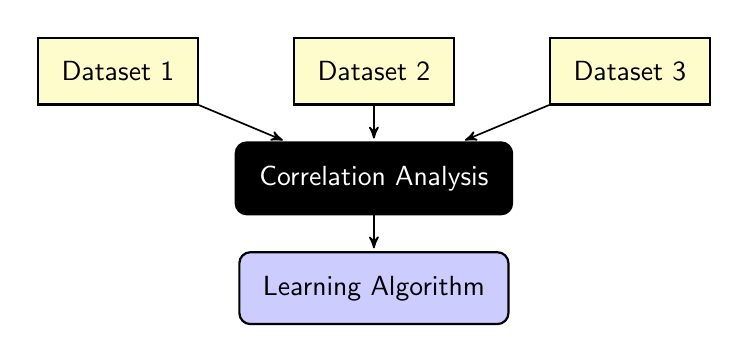
\begin{tikzpicture}[
      font=\sffamily, every matrix/.style={ampersand replacement=\&,column sep=3ex,row
      sep=3ex}, dataset/.style={draw,thick,fill=yellow!20,inner sep=.3cm},
      sink/.style={dataset,rounded corners,fill=black, text=white},
      app/.style={dataset,rounded corners,fill=blue!20}, dots/.style={gray,scale=2},
      to/.style={->,>=stealth',shorten >=1pt,semithick,font=\sffamily\footnotesize}, every
      node/.style={align=center}]

      \matrix{ \node[dataset] (dataset1) {Dataset 1}; \& \node[dataset] (dataset2)
        {Dataset 2}; \& \node[dataset] (dataset3) {Dataset 3}; \\

        \& \node[sink] (blackbox) {Correlation Analysis}; \& \\

        \& \node[app] (application) {Learning Algorithm}; \& \\ };

      \draw[to] (dataset1) -- (blackbox); \draw[to] (dataset2) -- (blackbox); \draw[to]
      (dataset3) -- (blackbox); \draw[to] (blackbox) -- (application);

    \end{tikzpicture}
    \caption{Illustration of multi-modal data fusion}
    \label{fig:data_fusion}
\end{center}
\end{figure}


\section{Canonical Correlation Analysis (CCA)}

\subsection{What is it? What is it not?}

Canonical correlation analysis (CCA) is a joint dimensionality reduction algorithm for
exactly two datasets that finds a linear transformation for each dataset such that the
correlation between the two transformed feature sets is maximized
\cite{hotelling1936relations}. CCA, however, \textit{is not} a data fusion algorithm. CCA
returns two linear transformations and a set of correlations. In this light, CCA is
extremely similar to principle component analysis (PCA), which returns a linear
transformation that accounts for the directions of largest possible variance in a
dataset. These principle components are typically used as features vectors in a variety of
machine learning algorithms. Just as PCA is a dimensionality reduction algorithm and not
the final machine learning algorithm that uses the principle components, CCA is a joint
dimensionality reduction algorithm whose dimensionality reduction ensures that datasets
are maximally correlated in their reduced spaces. These maximally correlated features may
then be used however a learning algorithm desires. 

The solution to CCA is easily found by solving a quadratic optimization problem. This
solution is a closed form expression relying on the singular value decomposition (SVD) of
a matrix product involving the covariance matrices of each dataset and the
cross-covariance between the two datasets. As these covariance matrices are rarely known
\textit{a priori}, practical uses of CCA rely on substituting sample covariance matrices
formed from training data, which we call empirical CCA.

The performance of empirical CCA has been studied previously, but insufficiently. When the
number of training samples is large compared to the dimensions of the datasets, the
performance is well understood \cite{gunderson1997estimating}. When the number of training
samples is less than the sum of the dimension of each dataset (sample deficient regime),
\cite{pezeshki2004empirical} proves that empirical CCA completely breaks down and always
reports a perfect correlation between the datasets. 

This extremely undesirable characteristic of empirical CCA has lead many to abandon CCA as
a reliable statistical analysis technique. Pezeshki, L.L. Scharf et al. argue that in this
sample deficient regime
\begin{quote}
  ... the \textcolor{red}{empirical canonical correlations are defective and
    may not be used} as     estimates of canonical correlations between random
  variables.\cite{pezeshki2004empirical}
\end{quote}
Similarly, Ge et al. conclude that
\begin{quote}
... CCA provide(s) \textcolor{red}{reliable information} about spatial
    correlations existing among pairs of data sets \textcolor{red}{only when SNRs ... are
    reasonably high, and the sample support is significantly larger than the data
    dimensions.}\cite{ge2009does}
\end{quote}



\subsection{Variations on CCA}

Due to this undesirable breakdown of CCA in the low-sample high-dimensionality regime,
many researchers proposed variations of CCA to avoid this performance loss. Most notably,
\cite{nadakuditi2011fundamental} used recent results from random matrix theory to
demonstrate that this performance breakdown may be avoided by trimming the sample
covariance matrix estimates to only include informative components. This algorithm is the
crux of this thesis. We will study its performance and develop theoretical tools in order
to use it for real-world applications. Throughout the thesis, we use the ubiquitous
low-rank signal-plus-noise model for datasets \be X = UV^H + Z, \ee where
$X=[x_1,\dots,x_n]$ is our observed data matrix whose columns are individual
multidimensional observations, $U$ is a low-rank signal subspace, $V$ is a low-rank signal
matrix, and $Z$ is a noise matrix. Surprisingly, correlation analysis for this classical
low-rank signal-plus-noise model is not completely studied. This thesis seeks to complete
the discussion. Here, we briefly touch on other variations based on CCA that do not assume
the above linear low-rank signal-plus-noise model. Many of these algorithms are tuned for
a specific application or seek to avoid the performance loss of CCA in a certain regime.

Regularized CCA (RCCA) \cite{vinod1976canonical} adds a penalty term to the magnitude of
the canonical vectors. This results in adding a scaled copy of the identity matrix to the
sample covariance matrix of each dataset, which allows each matrix to be
inverted. Therefore, RCCA returns non-trivial results in the sample-deficient
regime. However, this approach introduces a parameter to the algorithm; the effect of this
parameter is not well studied. Other variations of RCCA, such as supervised
RCCA \cite{thum2014supervised}, fast RCCA \cite{cruz2014fast}, and a multi-block RCCA
\cite{tenenhaus2014regularized}, have also been proposed.

Kernel CCA (KCCA) \cite{akaho2006kernel} was proposed to deal with non-linear correlations
existing between datasets. However, KCCA also introduces regularization parameters so as
to not return trivial solutions (see \cite{welling2005kcca} for an excellent
derivation). Besides the choice of regularization parameter, there is also ambiguity in
the choice of the kernel function, which is a common problem among kernel methods. Other
variations of KCCA have also been proposed, such as penalized KCCA
\cite{waaijenborg2009correlating}, alpha-beta divergence \cite{mandal2013non}, and CCA
based on kernel target alignment \cite{chang2013canonical}. 

Sparse CCA \cite{hardoon2011sparse} finds linear transformations such that the number of
features used is minimized. This problem is often motivated by the need for interpretable
canonical vectors that is often driven by the application, such as in brain imaging
\cite{yan2014accelerating}. There are many variations on sparse CCA, typically motivated
by application or mathematical intrigue. Sun and Keates \cite{sun2013canonical} explore
CCA in the context of censoring, Shin and Lee examine sparse functional data
\cite{shin2015canonical}, Tao et al. consider joint sparse data in
\cite{tao2014exploring}, Gao et al. explore efficient sparse CCA for high-dimensional
data \cite{gao2014efficient}, and Zhang et al. extend the analysis to multi-class group
sparse CCA \cite{zhang2013binary}. Other formulations include a penalized decomposition
\cite{witten2009penalized}, Bayesian CCA via group sparsity \cite{klami2013bayesian}, and
recursive sparse CCA \cite{chu2013sparse}.

\subsection{Applications}

CCA and its variants are widely used in a variety of fields where multiple datasets
naturally arise, the most common of which is machine learning and computer vision. In
\cite{hardoon2004canonical}, CCA is used to learn semantics of multimedia content by
fusing image and text data. Related, \cite{dhillon2011multi} uses CCA to learn word
embeddings for supervised natural language processing tasks. CCA has been widely applied
to pose estimation \cite{melzer2001nonlinear,zhai2015instance}, as this is a natural
examples where we have multiple views (image) of the same object. Other computer vision
related tasks where correlation methods are natural fits include matching people across
cameras \cite{lisanti2014matching}, clustering social event images
\cite{ahsan2014clustering}, automatic image annotation \cite{hardoon2006correlation}, and
audio-visual speaker clustering \cite{chaudhuri2009multi}.

Medical analysis is another field where there are ripe opportunities for correlation
analysis due to the vast number of modalities (EEG, MRI, CT, fMRI, MEG, etc.). CCA is
often used to determine interactions, or connectivities, between brain areas in fMRI data
\cite{deleus2011functional,arbabshirani2010comparison,khalid2013improving,guccione2013functional}
and used to fuse fMRI, sMRI, and EEG data \cite{correa2010canonical}. CCA based methods
have also been used to examine genetic connections
\cite{lin2013identifying,seoane2014canonical,lin2013group}, relying heavily on sparse
methods due to the high dimensionality of gene data and need to interpret which genes are
``on''. CCA is also a popular way to detect frequencies in steady-state visual evoked
potential (SSVEP) in brain-computer interfaces (BCIs)
\cite{zhang2013l1,nakanishi2014enhancing,zhang2014frequency}. Still further, CCA is used
in de-noising and analysis of EEG, MEG and ECG data
\cite{spuler2013spatial,campi2013non,chen2014removal,kuzilek2014comparison}.

CCA also has roots in classical signal processing applications. The authors of
\cite{via2005canonical} apply CCA to to the common communications problem of blind
equalization of single-input multiple-output (SIMO) channels. Pezeshki et al.
\cite{pezeshki2006canonical} showed that the CCA coordinates are the correct coordinates
for low-rank Gauss-Gauss detection and estimation. Scharf and Thomas
\cite{scharf1998wiener} provide a wonderful exposition on using the canonical coordinates
for Wiener filters, transform coding, filtering, and quantizing. CCA and multiset CCA have
been used to achieve joint blind source separation (BSS) in \cite{li2009joint}. CCA has
also been applied to hyperspectral imaging \cite{nielsen2002multiset}, array processing
\cite{ge2009does}, Gaussian channel capacity \cite{scharf2000canonical}, and cognitive
radio networks \cite{manco2014kernel}.

Other fun and interesting applications include climatology, finance, and music. Todros and
Hero define a new measure transformed based CCA and show its utility on financial data in
\cite{todros2012measure}. Torres et al. \cite{torres2007finding} use sparse CCA to label
portions of musical songs with meaningful words or phrases. In the field of climatology,
CCA has been used to study sea temperatures \cite{wilks2014probabilistic}, forest planning
\cite{prera2014using}, and tropical cyclones \cite{steward2014assimilating}. Finally, I
would be remiss if I didn't share my personal favorite application of CCA to date: using
CCA to analyze bovine growth \cite{li2010canonical}.

\section{Contributions of this thesis}

In many of the application presented above, researchers either have access to many
samples, or have designed an algorithm tuned specifically for a their particular
application. This thesis considers the performance of empirical correlation algorithms in
the low-sample, high dimensional setting. These algorithms are not geared toward a
particular application but are general and may be applied to any application. We will
demonstrate, both theoretically and empirically, that multi-modal correlation analysis in
this regime is a possibility. We remark that statements labeled as theorems represent, to
the best of our knowledge, new results while important results from literature are labeled
as propositions or lemmas. Chapters II-III are self contained and may be read
independently. Chapters IV-X consider the problem of correlation analysis.

Chapters \ref{sec:chpt_msd} and \ref{sec:chpt_msd_exten} consider the classical problem of
matched subspace detectors. We use insights from random matrix theory on the accuracy of
subspace estimates to derive new, optimal detectors that demonstrate the sub-optimality of
the classical plug-in detectors that simply substitute maximum likelihood estimates for
unknown parameters. Under both a stochastic and deterministic data model, we argue that
only the \textit{informative} subspace components should be used in a detector. We extend
this analysis to the case where our observations may contain missing data.

In Chapters \ref{sec:chpt_cca_det} and \ref{sec:chpt_cca_vects}, we explore the
performance of CCA and re-derive informative CCA (ICCA). We demonstrate the extreme
sub-optimality of CCA in the low-sample, high dimensionality regime. Specifically, we
provide a statistical test for both CCA and ICCA that determines whether the correlations
returned by the algorithms do indeed represent a true underlying correlation in the
datasets. We prove when each of these statistics are consistent to showcase the
superiority of ICCA. We also provide an analogous statistical test and consistency theorem
to use when the datasets have missing data entries. We create 3 new real-world,
multi-modal datasets involving video and audio to verify the performance of ICCA. We then
showcase that the canonical vectors returned by ICCA are more accurate than the CCA
vectors in the low-sample regime. Finally, we provide a new algorithm for estimating the
canonical vectors that asymptotically optimal.

Next, we explore the performance of regularized CCA (RCCA) in Chapter
\ref{sec:chpt_rcca}. When the number of training samples is limited but correlation
analysis is still desired, a common strategy is to regularize CCA by adding a penalty to
the magnitude of the linear transformation. However, we demonstrate that setting the
regularization parameter to infinity results in the best performance. In fact, in this
setting, the solution to RCCA may be found by taking the SVD of the sample
cross-covariance matrix between the two datasets. We then predict the behavior of the
largest singular values of this cross-covariance matrix assuming a low-rank
signal-plus-noise model on the individual datasets. We argue that using the top singular
values of this cross-covariance matrix to detect correlations is sub-optimal because the
correlation coefficients are coupled with the individual data signal strengths.

Using a similar proof technique, we predict the behavior of the largest singular values of
the projection of low-rank signal plus noise matrices to a smaller dimension in Chapter
\ref{sec:chpt_svd_proj}. Specifically, we consider two types of projection matrices: one
with standard complex Gaussian entries and one with orthonormal columns. We are able to
provide a closed form expression for the largest singular values in the case where the
projection matrix is unitary. Through numerical simulations, we demonstrate the
superiority of the unitary projection matrix over the Gaussian projection matrix. The
unitary projection matrix can reliably detect the signals at a lower signal-to-noise ratio
than the Gaussian projection matrix. 

In Chapter \ref{sec:chpt_det_reg} we apply CCA and ICCA to the classical problems of
detection and regression. First, we consider the low-rank signal-versus-noise subspace
detection problem given two datasets. We prove that the standard likelihood ratio test
(LRT) detector may be written using the canonical basis returned by CCA. We show that when
using empirical parameter estimates, the CCA detector is extremely suboptimal but that the
ICCA detector is equivalent to the plug-in LRT detector. We then show that the classical
Gaussian regression problem may be written in terms of the CCA basis. However, similar to
the detection problem, empirical CCA degrades the performance significantly while ICCA
matches the classical plug-in detector. We show this via mean squared error prediction
plots.

We then consider the joint problems of image retrieval and image annotation in Chapter
\ref{sec:chpt_ia}. Correlation based methods are typically overlooked as solutions to such
problems due to the problems with CCA outlined in this thesis. We show that using ICCA to
solve these problems results in non-trivial solutions. We compare the performance of CCA
and ICCA on four different image-text datasets and describe the capabilities and
limitations of ICCA in this application. When the datasets contain multiple images of the
same objects and meaningful captions, ICCA is able to capture correlations between images
and text. However, ICCA fails to capture semantic meanings between documents and
captions. We argue that with clever feature engineering and improved NLP techniques,
correlation based methods may be relevant for image retrieval and image annotation.

Lastly, we consider multi-set CCA (MCCA) in Chapter \ref{sec:chpt_mcca}. Unfortunately,
unlike CCA, there is no clear objective function to use in an optimization problem;
Kettenring \cite{kettenring1971canonical} proposes five such objective functions. Nielsen
also provides a nice formulation of MCCA in \cite{nielsen1994analysis} where he proposes
four constraint functions.  We provide derivations for these 20 formulations, in both a
theoretical and empirical setting. We then choose to consider the MAXVAR problem as we are
able to directly apply our insights from ICCA to create an informative version of it,
which we call informative MCCA (IMCCA). We demonstrate the superior performance of IMCCA
on a real-world video dataset that we created. 


\section{Problem Formulation}\label{sec:energy_detector}
We wish to design a detector that discriminates between the $H_0$ hypothesis that an
observation is purely noise and the $H_1$ hypothesis that the observation contains an
unknown signal.  We model the observation $w\in\reals^{k\times 1}$ as in
(\ref{eq:general_setup}) where $\delta=[\delta_1,\dots,\delta_k]^T\in\reals^{k\times 1}$,
with $\delta_i\neq 0$, is an unknown deterministic vector,
$z\sim\mathcal{N}\left(0,I_k\right)$ is additive white Gaussian noise (AWGN), and $k$ is
known. See
\cite{cui2013performance,santiago2013noise,arribas2013antenna,chen2013adaptive,gorji2013widely,zhou2013space,kwon2013multi,hu2013doa,liao2013direction}
for similar signal-plus-noise models in signal and array processing.  In the
Neyman-Pearson detection setting (see \cite{van1968detection}), the detector for this data
model is the likelihood ratio test (LRT)
\beq\label{eq:lrt_form}
\Lambda(w) = \frac{f\left(w\,|\, H_1\right)}{f\left(w\,|\, H_0\right)} \detgtrless \eta.
\eeq
Here $f\left(\cdot\right)$ is the appropriate conditional probability density function
(p.d.f.) of the observation and $\eta$ is a scalar threshold set so that $\Prob{\Lambda(w)
  > \eta\,|\, w\in H_0} = \alpha$ where $\alpha\in[0,1]$ is a desired false alarm rate.

The conditional distributions of $w$ modeled as in (\ref{eq:general_setup}) are
$w|H_0\sim\mathcal{N}\left(0,I_k\right)$ and
$w|H_1\sim\mathcal{N}\left(\delta,I_k\right)$. However, as $\delta$ is unknown, we cannot
substitute the p.d.f. of $w|H_1$ into (\ref{eq:lrt_form}). Instead, we use the generalized
LRT (GLRT), which maximizes $f(w|H_1)$ with respect to any unknown parameters. The GLRT
for our problem is 
\be \Lambda(w) = \frac{\max_{\delta}f\left(w\,|\,
    H_1\right)}{f\left(w\,|\, H_0\right)} \detgtrless \eta.  
\ee
The conditional p.d.f. of $w$ under the $H_1$ hypothesis is
\be
f\left(w\,|\,H_1\right) = \left(2\pi\right)^{-k/2}\exp\left\{ -\frac{1}{2}\left(w-\delta\right)^T\left(w-\delta\right)\right\}.
\ee
This p.d.f. is maximized when $\delta=w$ with the maximum value of
$(2\pi)^{-k/2}$. Substituting this into the GLRT yields
\be
\Lambda(w) = \exp\{\frac{1}{2}w^Tw\}
\ee
Taking the natural logarithm results in the test statistic
\beq\label{eq:energy_detector}
\Lambda_{\text{energy}}(w) = w^Tw = \sum_{i=1}^k w_i^2
\eeq
where $w=[w_1,\dots,w_k]^T$. This is an energy detector as its test statistic sums the
energy residing in each component (or dimension) of the given observation.

\subsection{ROC Curve Analysis}

To compare the performance of multiple detectors, we will compare their receiver operating
characteristic (ROC) curves. A ROC curve is a collection of points ($P_F,P_D$) where for
$-\infty<\eta<\infty$,
\beq\label{eq:roc}\ba
&P_F=\Prob{\Lambda(w) > \eta \,|\, w\in H_0},\\
&P_D=\Prob{\Lambda(w) > \eta \,|\, w\in H_1}.\\
\ea\eeq
For $0\leq P_F\leq 1$ we want to express the probability of detection $P_D$ as a function
of the false alarm rate, $P_F$, while noting that $P_F$ is a function of
$\eta$. To make analytical progress, we assume that $\delta$ is known for ROC
derivations. First, we compute the conditional distributions of the statistic in
(\ref{eq:energy_detector}). The conditional distributions of the components in $w$ are
simply 
$w_i|H_0\overset{\text{i.i.d.}}{\sim}\mathcal{N}\left(0,1\right)$ and
$w_i|H_1\overset{\text{i.i.d.}}{\sim}\mathcal{N}\left(\delta_i,1\right)$. Therefore,
$w_i^2|H_0\overset{\text{i.i.d.}}{\sim}\chi^2_1$ and
$w_i^2|H_1\overset{\text{i.i.d.}}{\sim}\chi^2_1\left(\delta_i^2\right)$ where $\chi^2_1$
is a chi-square random variable with one degree of freedom and $\chi^2_1(\delta_i^2)$ is a
non-central chi-square random variable with one degree of freedom and non-centrality
parameter $\delta_i^2$. As each component $w_i$ is independent,
\beq\label{eq:distr_energy} \ba
&\Lambda(w)|H_0\sim\chi^2_k,\\
&\Lambda(w)|H_1\sim\chi^2_k\left(\delta^T\delta\right), 
\ea \eeq 
where $\chi^2_k$ is a chi-square random variable with $k$ degrees of freedom and $\chi^2_k(\delta^T\delta)$ is a
non-central chi-square random variable with $k$ degrees of freedom and non-centrality
parameter $\delta^T\delta = \sum_{i=1}^k\delta_i^2$. Armed with these characterizations in
(\ref{eq:distr_energy}) and solving for $\eta$ in (\ref{eq:roc}), we can relate $P_D$ to
$P_F$ using the expression
\begin{equation}\label{eq:roc_energy}
\begin{aligned}
&P_{D_\text{energy}}(P_F,k)=1-Q_{\chi_{k}^2(\lambda_k)}\left(Q^{-1}_{\chi^2_{k}}\left(1-P_F\right)\right).\\
\end{aligned}
\end{equation}
In (\ref{eq:roc_energy}), $Q_{\chi_{k}^2}(\lambda_k)$ is the cumulative distribution function (c.d.f.) of a
non-central chi-square random variable with $k$ degrees of freedom and non-centrality
parameter $\lambda_k=\sum_{i=1}^k\delta_i^2$ and $Q_{\chi_{k}^2}$ is the c.d.f. of a chi-square random
variable with $k$ degrees of freedom. See \cite{cui2013performance,arribas2013antenna,zhou2013space} for similar ROC
performance curve derivations.

\subsection{Problem Statement}\label{sec:prob_state}

As practitioners, we can control which signal components that the energy detector in
(\ref{eq:energy_detector}) uses. Without loss of generality, we assume that the entries of
$\delta$ are ordered (i.e. $|\delta_1| \geq |\delta_2| \geq\dots|\delta_k|$). With this
assumption, we can decide how many signal components, $d$, to use in the energy detector
\beq\label{eq:the_detector} 
\Lambda_d(w) = \sum_{i=1}^d w_i^2.
\eeq 
Specifically, we wish to answer the following question:
\begin{quote}
  Given a signal vector $\delta$ and a desired false alarm rate $P_F$, how many signal
  components, $d$, maximize $P_{D_{\text{energy}}}(P_F,d)$ in (\ref{eq:roc_energy}) for an
  energy detector with the form of (\ref{eq:the_detector}) derived from observations
  as in (\ref{eq:general_setup})? 
\end{quote}
Answering this question will provide some surprising results. We will show that if the
components $\delta_i$ are too small in magnitude, including them in a detector actually
degrades performance. The setting where $\delta_i$ equals zero is a special case where not
including it will always yield a performance gain.

\section{Useful Components In Energy Detectors}\label{sec:useful}
In this section, we answer the question posed at the end of Section
\ref{sec:energy_detector} by defining $\kuse$, the number of useful signal components. We
show that $\kuse$ is dependent on $\delta$ and the desired false alarm rate $P_F$. We
provide some intuition behind our definition by discussing how the conditional
distributions of the energy detector's test statistic shift when adding additional
components. If an additional signal component further separates the conditional
distributions, it is one of the $\kuse$ components in detection; otherwise, including that
component would degrade detector performance. Of particular importance, $\kuse$ may be
less than the inherent dimension, $k$, of the observed data, even when $\delta_i\neq0$.

\subsection{Definition and Computation of $\kuse$}

We define the number of useful detection components at a false alarm rate $P_F$ as the
solution to the following optimization problem
\beq\label{eq:opt_prob}
\kuse = \argmax_{d\in\{1,\dots,k\}} P_{D_{\text{energy}}}(P_F,d)
\eeq 
where $P_{D_{\text{energy}}}(P_F,d)$ is defined in (\ref{eq:roc_energy}). This is the
optimal number of components to include in an energy detector in (\ref{eq:the_detector})
to maximize detector performance. Using exactly $\kuse$ components includes all components
that improve detection ability and excludes all components that degrade detection ability.

To determine $\kuse$, we propose the greedy ``algorithm'' in Figure \ref{algo:kuse}. The
algorithm relies on the fact that the components of $\delta$ are ordered
(i.e. $|\delta_1|\geq\dots|\delta_k|$). It adds one component at a time and searches for
the last component that resulted in an increase in detection ability. This algorithm
relies on knowledge of $\delta$ and so by definition $\kuse$ is an oracle quantity.
Therefore, a realizable detector using exactly $\kuse$ components is currently beyond
reach. Estimating $\kuse$ is a topic for future work and may involve placing a prior
distribution on the test vector. In Section \ref{sec:msd}, we discuss using the effective
number of subspace components, $\keff$, as an estimate for $\kuse$.

%\begin{figure}
% \hrulefill
%  \begin{algorithmic}[1]


\begin{algorithm}
  \KwIn{$P_F$, $\delta$ }

  Compute $P_D(P_F,1)$ from (\ref{eq:roc_energy})

  \For{$h=2,\dots,k$} {

    Compute $P_D(P_F,h)$ from (\ref{eq:roc_energy})

    \If{$P_D(P_F,h) < P_D(P_F,h-1)$}{

      $\kuse= h-1$

      \textbf{Return:} $\kuse$
    }
  }
  $\kuse = k$

  \KwOut{$\kuse$ }
  \caption{Algorithm to determine $\kuse$. This is computable in an oracle setting\\
    where $\delta$ is known.}  
  \label{algo:kuse}
\end{algorithm}

\subsection{Discussion of Test Statistic Distributions}

In order to provide intuition behind the definition of $\kuse$, we examine the conditional
distribution of the test statistic in (\ref{eq:the_detector}):
\beq\label{eq:d_distrs}\ba
& \Lambda_d(w)\,|\,H_0 \sim\chi^2_d,\\
& \Lambda_d(w)\,|\,H_1 \sim\chi^2_d(\lambda_d)\\
\ea\eeq
where
\beq\label{eq:nc_param}
\lambda_d = \sum_{i=1}^d \delta_i^2.
\eeq
Clearly, both distributions and the non-centrality parameter depend on $d$. Therefore, a
closed form expression for $\kuse$ is not possible and we rely on the greedy algorithm
in Figure \ref{algo:kuse}. Adding an additional component presents a tradeoff between
adding $\delta_i^2$ to the non-centrality parameter and adding 1 to the degrees of
freedom in the c.d.f's in (\ref{eq:d_distrs}).

This tradeoff becomes more evident when using (\ref{eq:roc_energy}) to rewrite the
optimization problem in (\ref{eq:opt_prob}) as
\beq\label{eq:simple_opt}
\kuse = \argmin_{d\in\{1,\dots,k\}}
Q_{\chi_{d}^2(\lambda_d)}\left(Q^{-1}_{\chi^2_{d}}\left(1-P_F\right)\right). 
\eeq

By fixing the signal distribution $Q_{\chi^2_d(\lambda_d)}$, solving (\ref{eq:simple_opt}) is
equivalent to minimizing $Q^{-1}_{\chi^2_{d}}\left(1-P_F\right)$, which is achieved when
$d=1$. This minimizes the variance contribution from the noise distribution. However, by
fixing the noise distribution $Q_{\chi^2_d}$, solving (\ref{eq:simple_opt}) is equivalent
to minimizing $Q_{\chi_{d}^2(\lambda_d)}\left(\cdot\right)$, which is achieved when
$d=k$. This maximizes the variance contribution from the signal distribution. The solution
to (\ref{eq:simple_opt}) is dependent on how much each additional component contributes to
the overall non-centrality parameter. If the contribution is large enough, the added
variance in the noise distribution from the extra degree of freedom is overcome by the
distribution shift induced by the increase in non-centrality parameter.

To illustrate how the conditional distributions shift when adding components to the energy
detector, Figure \ref{fig:distributions} plots the distributions of $\Lambda_d(w)|H_0$ and
$\Lambda_d(w)|H_1$ for three choices of $d$ and $\lambda_d$. Figure \ref{fig:small} sets
$d=1$ and $\lambda_d=2$ and is used as a baseline. Figure \ref{fig:med} increases the
number of components to $d=2$ while keeping the non-centrality parameter fixed at
$\lambda_d=2$. The added component increases the noise variance by 2. However, as there is
no increase in the non-centrality parameter, the signal variance also increases by
2. Thus, the signal-to-noise ratio is effectively decreased. Therefore, the second
component causes the conditional distributions to become more similar and thus degrades
detector performance; therefore, $\kuse=1$. Figure \ref{fig:big} keeps the number of
components at $d=2$ but increases the non-centrality parameter to $\lambda_d=3$. In this
setting, the increase in non-centrality parameter increases the signal variance, which
overcomes the resulting increase in noise variance. The second component further separates
the conditional distributions and improves detection performance; therefore,
$\kuse=2$. Figure \ref{fig:dist_roc} plots the corresponding ROC curves for the three
choices of parameters in Figure \ref{fig:distributions}. When adding a component causes
the conditional distributions to better separate as in Figure \ref{fig:big}, the resulting
ROC curve shows an improvement in detection. \textit{For an additional component to be one
  of the $\kuse$ components, the resulting increase in noise variance must be overcome by
  a sufficiently large enough increase in non-centrality parameter.}

\begin{figure}[t]
\centering
\subfigure[$d=1$, $\lambda_d=2$]{
  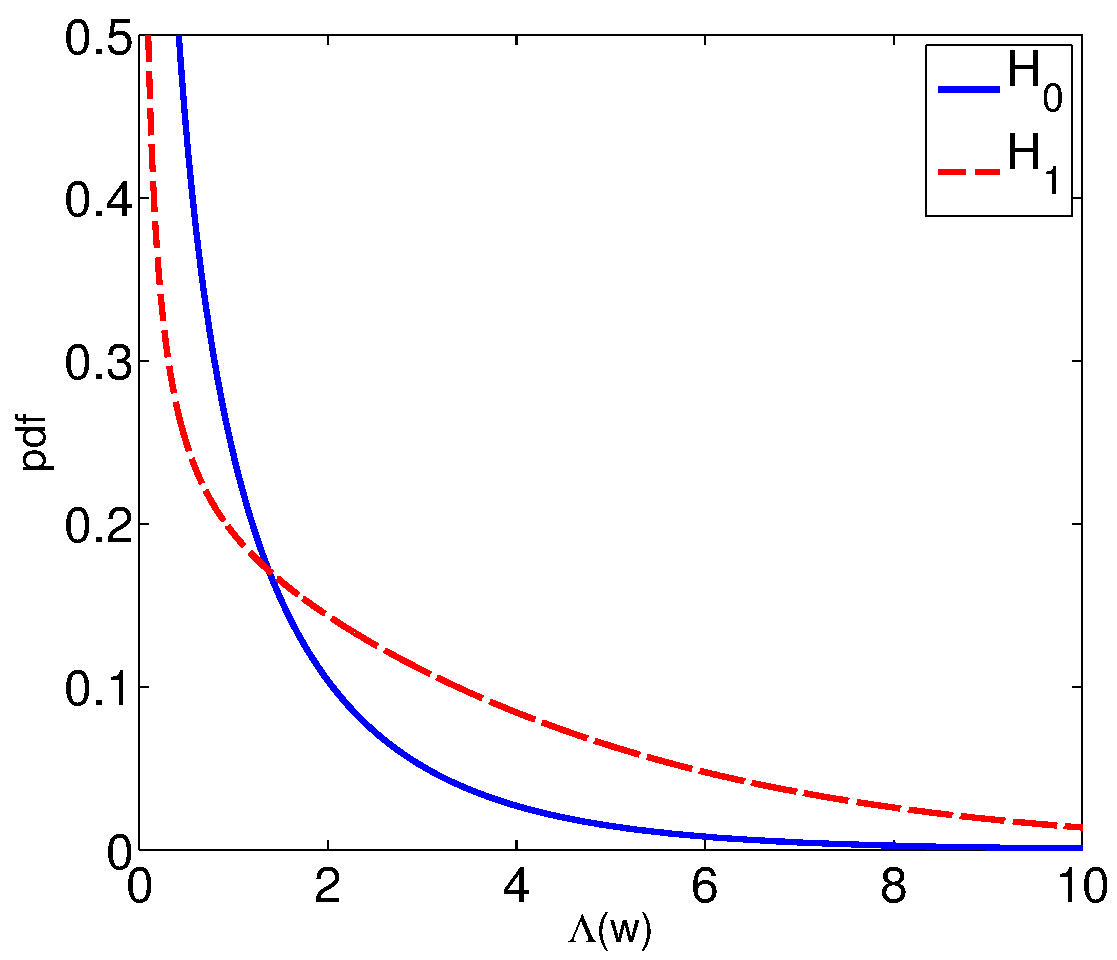
\includegraphics[width=0.3\textwidth]{taes_msd/figures/dist1.pdf}
  \label{fig:small}}
\subfigure[$d=2$, $\lambda_d=2$]{
  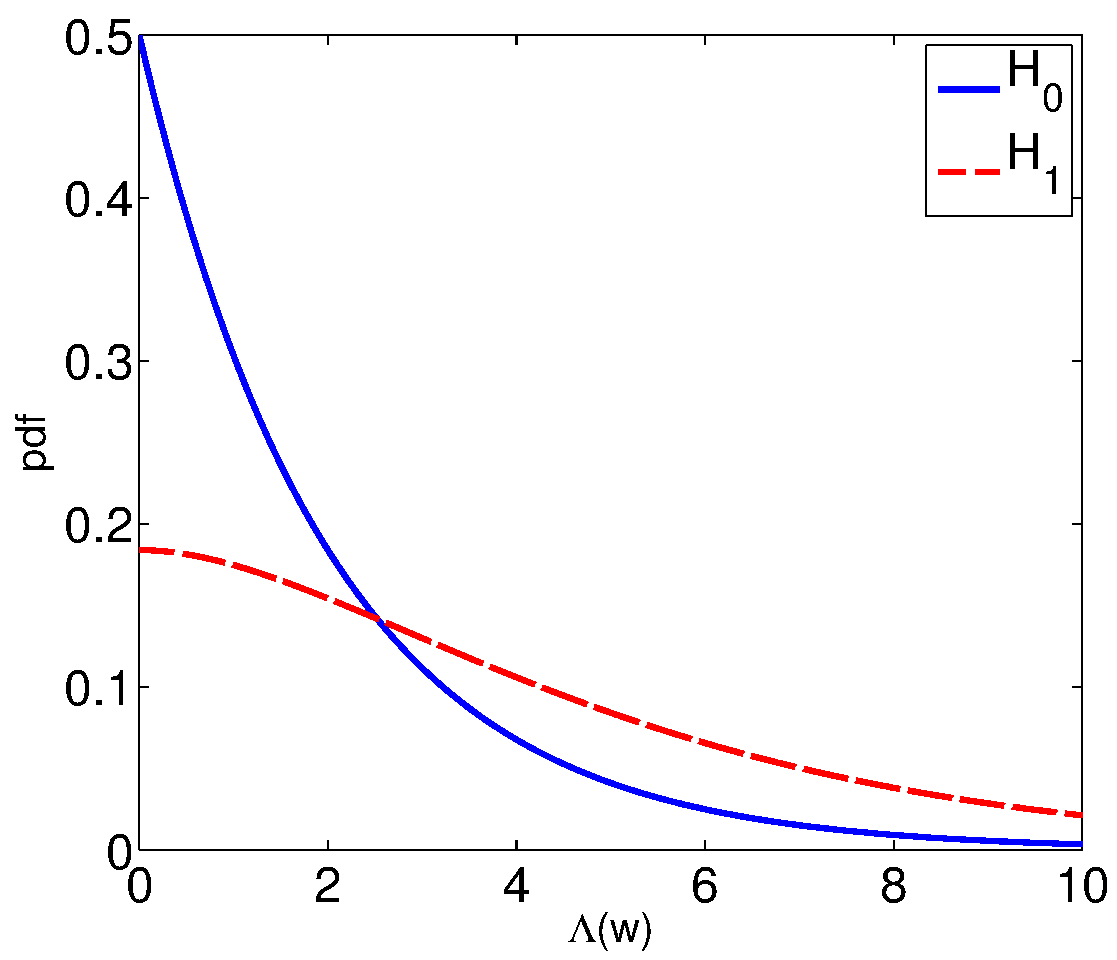
\includegraphics[width=0.3\textwidth]{taes_msd/figures/dist2.pdf}
  \label{fig:med}}
\subfigure[$d=2$, $\lambda_d=3$]{
  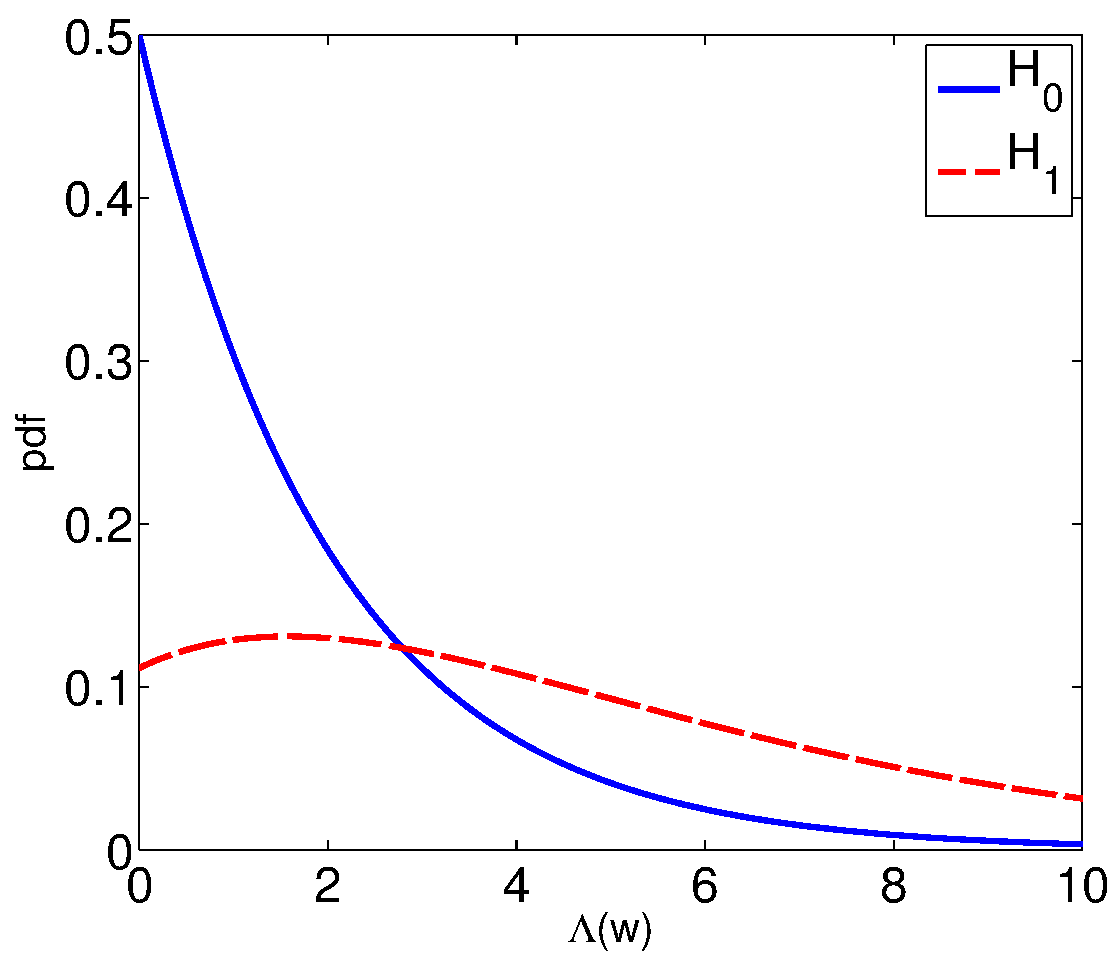
\includegraphics[width=0.3\textwidth]{taes_msd/figures/dist3.pdf}
  \label{fig:big}}
\caption{Probability density function (p.d.f.) of $\Lambda(w)\,|\,H_0$ and
  $\Lambda(w)\,|\,H_1$ for three combinations of the number of components $d$ and
  non-centrality parameter $\lambda_d$. (a) Baseline: $d=1$, $\lambda_d=2$ (b) Increases $d$
  but keeps $\lambda_d$ fixed. The distributions are less separable. (c) Increases both $d$
  and $\lambda_d$. The distributions are more separable.}
\label{fig:distributions}
\end{figure}

\begin{figure}[t]
  \centering
  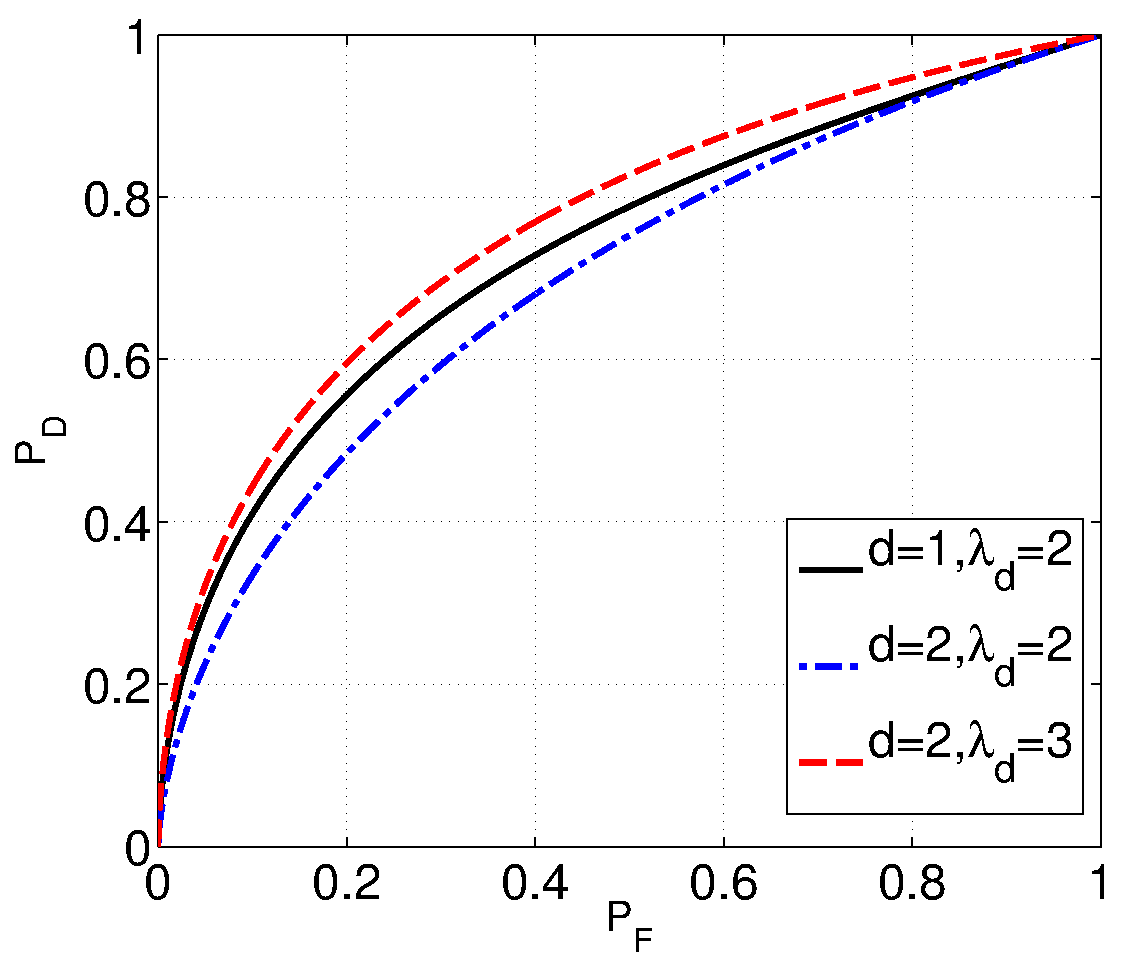
\includegraphics[width=\figwidth]{taes_msd/figures/dist_roc.pdf}
  \caption{The corresponding ROC curves to the three choices of $d$ and $\lambda_d$ in
    Figure \ref{fig:distributions}. ROC curves were generated from (\ref{eq:roc}). When
    adding an additional subspace component, the non-centrality parameter must increase
    sufficiently in order to achieve improved detection. }
  \label{fig:dist_roc}
\end{figure}

Finally, we explore the minimum increase in non-centrality parameter needed to improve
detection ability. Consider a setting with $d=1$ component and corresponding
non-centrality parameter $\lambda_1$. Let $\lambda_2$ be the resulting non-centrality
parameter by adding a second component, $d=2$, and let $\Delta\lambda=\lambda_2-\lambda_1$
be the resulting increase in non-centrality parameter. Figure \ref{fig:nc_lines} plots the
minimum increase in non-centrality parameter needed to improve detection as a function of
$\lambda_1$ for a few choices of $P_F$. If the increase in non-centrality parameter
exceeds this minimum threshold, that component is one of the $\kuse$ components.

We observe that the minimum increase in non-centrality parameter is dependent both on the
desired false alarm rate, $P_F$, and the first non-centrality parameter, $\lambda_1$.

The minimum increase in non-centrality parameter is larger for smaller false alarm rates
and is larger for larger $\lambda_1$. This is intuitive because larger values of
$\lambda_1$ separate the conditional distributions very well, indicating that the first
component is an excellent discriminant between the two hypotheses $H_0$ and $H_1$. For the
second component to improve detection ability, its contribution to the non-centrality
parameter must be larger for larger $\lambda_1$. Otherwise, the second component only adds
more noise to the detector. More generally, for the $i$th component to be one of the
$\kuse$ components, $\delta_i^2$ must exceed a critical threshold that is dependent on
$\sum_{j=1}^{i-1}\delta_j^2$. 

\begin{figure}[t]
\centering
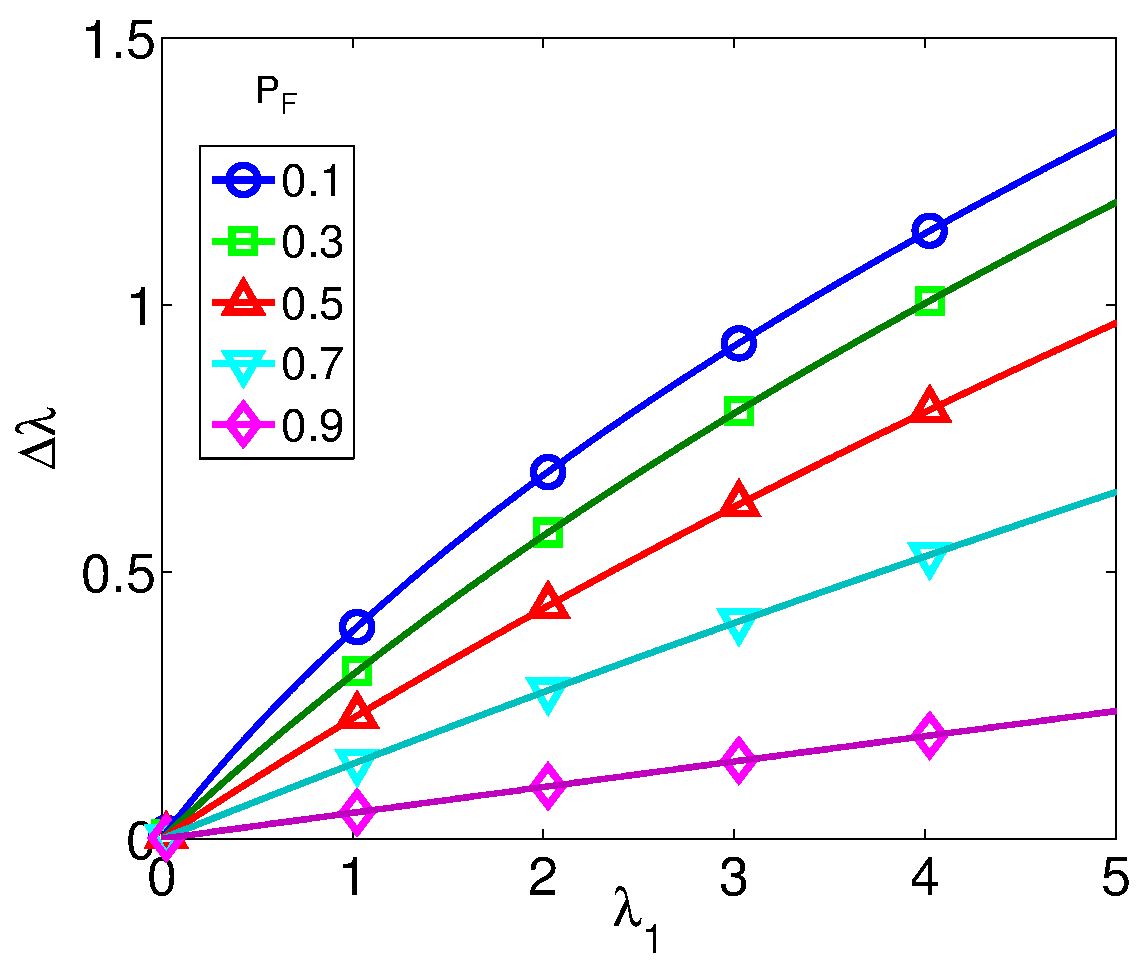
\includegraphics[width=\figwidth]{taes_msd/figures/nc_lines.pdf}
\caption{Minimum increase in non-centrality parameter necessary for increased detector
  performance. Results are shown for multiple choices of $P_F$. $\lambda_1$ indicates the
  non-centrality parameter when $d=1$ and $\Delta\lambda$ indicates the increase in
  non-centrality parameter when increasing the number of components to $d=2$.}
\label{fig:nc_lines}
\end{figure}


\section{Useful Components in Deterministic Matched Subspace Detectors}\label{sec:msd}
This section will apply the results in Section \ref{sec:useful} about useful components to
deterministic matched subspace detection. In this detection setting, we are given a high
dimensional test observation and wish to discriminate between the $H_0$ hypothesis that
the observation is purely noise and the $H_1$ hypothesis that the observation contains a
low-rank-$k$ signal that lies at a fixed point in an unknown subspace. To design a
detector, we have access to a training dataset of signal bearing observations.
We assume that the training data was collected in a variety of representative experimental
conditions, allowing each observation's signal component to lie at a different location in
the signal subspace. This setup is the similar to that in \cite{asendorf2013performance}
and the resulting standard matched subspace detector is an energy detector with the same
form as (\ref{eq:the_detector}). We use random matrix theory to determine the number of
informative subspace components, $\keff$, which is an upper bound for
$\kuse$. Through a numerical example, we demonstrate the relationship between the standard
plug-in detector using exactly $k$ subspace components, a detector using $\keff$ subspace
components, and a detector using exactly $\kuse$ subspace components.

\subsection{Training Data Model}\label{sec:training_data}

Let $U=[u_1,\dots,u_k]\in\reals^{n\times k}$ be an unknown signal subspace matrix with
pairwise orthonormal columns $u_i\in\reals^{n\times 1}$. To estimate $U$, 
we are provided a dataset containing $m$ signal-bearing training vectors
$y_i\in\reals^{n\times 1}$, $i=1,\dots,m$, modeled as 
\beq\label{eq:taes_train}
y_i=Ux_i+z_i 
\eeq 
where
$z_i\overset{\text{i.i.d.}}{\sim}\mathcal{N}(0,I_n)$ and
$x_i\overset{\text{i.i.d.}}{\sim}\mathcal{N}(0,\Sigma)$ where
$\Sigma=\diag(\sigma_1^2,\dots,\sigma_k^2)\in\reals^{k\times k}$ with
$\sigma_1>\sigma_2>\dots>\sigma_k>0$ known. For each observation, $x_i$ and $z_i$ are
independent. In the training data, $x_i$ is modeled stochastically to represent the
variety of conditions under which the training data may be collected.  We assume that the
dimension, $k$, of our subspace is known and that $k\ll n$ so that we have a low-rank
signal embedded in a high-dimensional observation vector. Applications in which training
datasets arise include MIMO radar \cite{chen2013adaptive}, GNSS receivers
\cite{arribas2013antenna}, source localization \cite{he2013near}, DOA
\cite{liao2013direction}, and target detection \cite{kwon2013multi}. In such applications,
we may think of the entries of $y_i$ received data from an antenna array, $U$ as the
channel response matrix, $x_i$ as the transmitted waveform, $\Sigma$ as the signal-to-noise
ratio (SNR) matrix, and $z_i$ as additive noise.

\subsection{Testing Data Model}

In the testing setting, we are given an unlabeled observation $y\in\reals^{n\times 1}$
modeled as
\begin{equation}\label{eq:determ_setup}
y=\left\{
\begin{aligned}
&z
&& y\in H_0:\text{ Noise only}\\
&U\Sigma^{1/2} x+z
&& y\in H_1:\text{ Signal-plus noise}\\
\end{aligned}\right. ,
\end{equation}
where $U$, $\Sigma$, and $z$ are modeled the same as the training data as described in
Section \ref{sec:training_data}. However, for the test observations, $x=[x_1,\dots,x_k]^T$
is a non-random, unknown deterministic vector. Thus the signal, $U\Sigma^{1/2}x$, lies at a
fixed point in the unknown subspace. Note that $\Sigma$ controls the SNR of each subspace
component.

\subsection{Subspace Estimation and Accuracy}\label{sec:param_estim}

In the testing model, the signal subspace $U$ is unknown and must be estimated from the
provided training data. Given the signal bearing training data 
\be
Y = \left[ y_1, \dots, y_m \right]\in\reals^{n\times m},
\ee 
we form the sample covariance matrix
$S=\frac{1}{m}YY^{T}$. The covariance matrix of a training observation is $\E{y_iy_i^T} = U\Sigma
U^T +I_n$ and it follows that the (classical) maximum likelihood estimates (in the many-sample, small
matrix setting) for $U$ is given by 
\beq\label{eq:param_estims_stoch}
\widehat{U}=[\widehat{u}_1 \dots \widehat{u}_{k}] \eeq
where
$\widehat{u}_1,\dots,\widehat{u}_{k}$ are the eigenvectors of $S$ corresponding to the
largest $k$ eigenvalues \cite{muirhead1982aspects} .

In any real world setting, we have finite training data and finite SNR. Therefore,
$\widehat{U}$ is inaccurate and degrades the performance of any detector that relies on it.
Proposition 5.1 of \cite{asendorf2013performance}  characterized the asymptotic accuracy of the
eigenvectors of the sample covariance matrix $S$ stating that as $n,m\to\infty$ with $c=n/m$
\beq\label{eq:angles}
|\langle u_i,\widehat{u}_i\rangle|^2 \convas
\begin{cases}
\dfrac{\sigma_i^4-c}{\sigma_{i}^4+\sigma_{i}^2c} & \text{ if } \sigma_{i}^2>\sqrt{c}\\
0 & \textrm{otherwise}\\
\end{cases}.  \eeq We note that $\convas$ denotes almost sure convergence. The key insight
to (\ref{eq:angles}) is that only the eigenvectors corresponding to the signal variances,
$\sigma_i^2$, lying above the phase transition $\sqrt{c}$ are
\textit{informative}. Following \cite{asendorf2013performance, nadakuditi2008sample}, we
define the effective number of (asymptotically) identifiable subspace components
$k_\text{eff}$ as:
\begin{equation}\label{eq:keff}
k_\text{eff} = \text{Number of } \sigma_i^2 > \sqrt{c}.
\end{equation}

\subsection{Plug-in and RMT Detectors}

If $U$ was known, the matched subspace detector is the GLRT using the test statistic (see
\cite{scharf1994matched,vincent2008matched,fuchs2007robust})
\be
\Lambda(w) = y^TUU^Ty = w^Tw
\ee
where $w=U^Ty\in\reals^{k\times 1}$. This is clearly an energy detector of the same form as
(\ref{eq:the_detector}) where each component of $w$ is the energy of $y$ residing in that
direction of the subspace. However, this detector is not realizable as $U$ is unknown and
so we substitute $\widehat{U}$ for the unknown $U$, resulting in the plug-in detector
\cite{asendorf2013performance}
\beq\label{eq:plugin_stat}
\Lambda_{\text{plugin}}(\widehat{w})= \widehat{w}^T\widehat{w} = \sum_{i=1}^k \widehat{w}_i^2
\eeq 
where $\widehat{w} = \widehat{U}^T y$ is the projection of the test observation onto the
estimated subspace. Similar plug-in techniques using sample covariance matrices occur in
direction detection \cite{santiago2013noise} and GNSS receivers \cite{arribas2013antenna}. The plug-in detector incorrectly assumes that $\widehat{U}=U$ and consequently
that all $k$ subspace components are informative. To avoid some of the performance loss of the
plug-in detector associated with including uninformative subspace components, we derived a
RMT detector that only includes the informative subspace components (see \cite{asendorf2013performance} for a derivation). The
RMT detector statistic is 
\beq\label{eq:rmt_stat}
\Lambda_{\text{rmt}}(\widehat{w})= \sum_{i=1}^{\keff}\widehat{w}_i^2.
\eeq

Clearly, both the plug-in and RMT detectors are energy detectors of the form in 
(\ref{eq:the_detector}) and so we may use (\ref{eq:roc_energy}) to analyze the performance
of each detector. In the MSD application, $\delta_i = \sigma_i|\langle
u_i,\widehat{u}_i\rangle| s_i x_i$ where $s_i\in\left\{1,-1\right\}$ represents the
random phase ambiguity in the eigenvector computation. Therefore, the non-centrality
parameter for this problem is 
\beq\label{eq:msd_nc_param}
\lambda_d = \sum_{i=1}^d \sigma_i^2|\langle u_i,\widehat{u}_i\rangle|^2x_i^2
\eeq
where the plug-in detector uses $d=k$ subspace components and the RMT detector uses
$d=\keff$ subspace components. In \cite{asendorf2013performance}, we demonstrated that the
plug-in detector is suboptimal and that the RMT detector will always achieve the same or
better performance.

\subsection{Relationship between $\kuse$ and $\keff$}

We first note that $\kuse\leq\keff$. If a subspace component is uninformative ($|\langle
u_i,\widehat{u}_i\rangle|^2 =0$ as determined by (\ref{eq:keff})), that component
contributes nothing to the non-centrality parameter as defined in
(\ref{eq:msd_nc_param}). From the analysis in Section \ref{sec:useful}, including this
subspace component in a detector would degrade detector performance. Therefore, a subspace
component must be informative to be one of the $\kuse$ subspace components. 

However, the number of useful subspace components may be strictly less than the number of
informative subspace components. As demonstrated in Figure \ref{fig:nc_lines}, when adding
an additional subspace component, the increase in non-centrality parameter must exceed a
minimum value. Examining (\ref{eq:msd_nc_param}), the non-centrality parameter depends on
$\Sigma$, $x$, and the accuracy of the eigenvectors of the sample covariance matrix
($|\langle u_i, \widehat{u}_i\rangle|^2$). Depending on these values, adding the $i$-th
component may not increase the non-centrality parameter enough to improve detection, even
when the subspace component is informative ($|\langle u_i,
\widehat{u}_i\rangle|^2>0$). Thus, it is possible for informative subspace components to
not be useful in detection.

Besides the desired false alarm rate, $P_F$, $\kuse$ also depends on $\Sigma$ and $x$ for
the matched subspace detector. Larger values of $|x_i|$ and $\sigma_i$ lead to larger
non-centrality parameters as defined in (\ref{eq:msd_nc_param}), making it more likely for
that component to be useful.  This is intuitive because the larger $|x_i|$ and $\sigma_i$
force the mean of the conditional distribution of $\widehat{w}_i|H_1$ further from 0,
which is the mean of the conditional distribution of $\widehat{w}_i|H_0$.  If we
instead fix $\Sigma$, $n$ , and $x$ and allow $m$ to change, we observe that more training
data increases the accuracy the subspace estimate as seen in (\ref{eq:keff}). Therefore,
increasing $m$ increases $\delta_i$, which may make subspace components useful.

The number of informative subspace components, $\keff$, is an upper bound for the number
of useful subspace components, $\kuse$. As mentioned earlier, we cannot compute $\kuse$ in
closed form because the deterministic vector $x$, which drives the non-centrality
parameters $\delta_i$, is unknown. Therefore, $\kuse$ is an oracle statistic as so we use
$\keff$ as a proxy for $\kuse$ in a realizable detector. However, as $\keff$ does not depend
on $x$, whenever $\keff\neq\kuse$, detectors using $\keff$ subspace components will be
suboptimal.

Finally, we note that the derivation and computation of $\kuse$ for the matched subspace
detection application relies on random matrix theory. Without these insights, we would
have no expression for $|\langle u_i,\widehat{u}_i\rangle|^2$ and subsequently could not
compute the non-centrality parameter in (\ref{eq:msd_nc_param}) to use in the algorithm in
Figure \ref{algo:kuse}.

\subsection{Numerical Example}

In Figure \ref{fig:main_result} we compare the performance of the plug-in and RMT
detectors to the performance of a detector that uses $d=\kuse$ subspace components. We
consider the setting when $k=3$, $n=200$, $\Sigma=\diag(5,2,0.5)$, and
$x=[1.5,1.5,1.5]^T$. For a fixed $P_F=0.1$, Figure \ref{fig:det_perf} plots the
theoretical detection probability (as computed in (\ref{eq:roc_energy}) using
(\ref{eq:keff}) and (\ref{eq:msd_nc_param})) given various amounts of training
data. Results are shown for the plug-in ($d=k$), RMT ($d=\keff$), and useful ($d=\kuse$)
detectors. Figure \ref{fig:dvals} plots the
corresponding number of subspace components each uses given various amounts of training
data.

\begin{figure}[t]
\centering
\subfigure[Detector Performance]{
  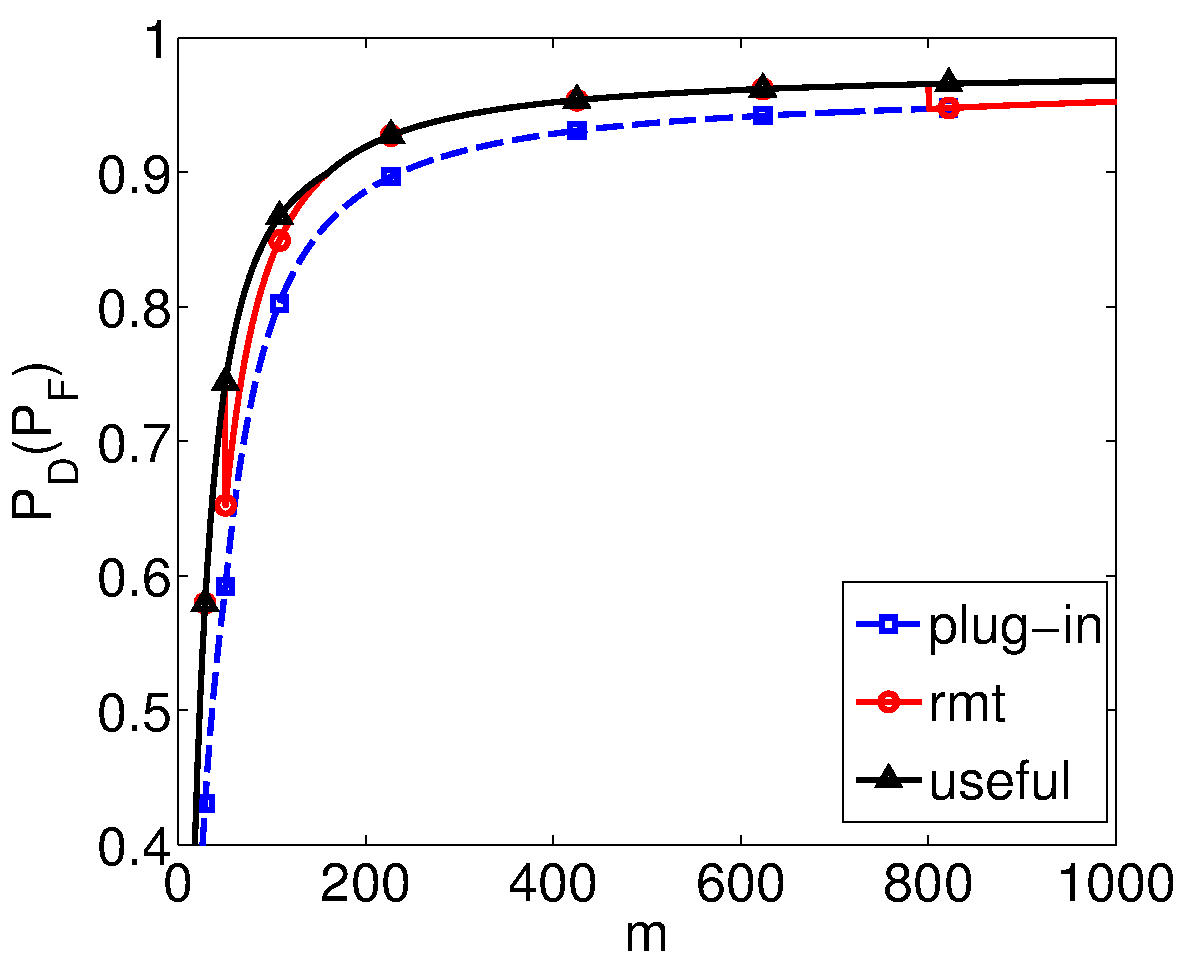
\includegraphics[width=0.45\textwidth]{taes_msd/figures/taes_pd_v_m.pdf}
  \label{fig:det_perf}}
\subfigure[Number of Subspace Components]{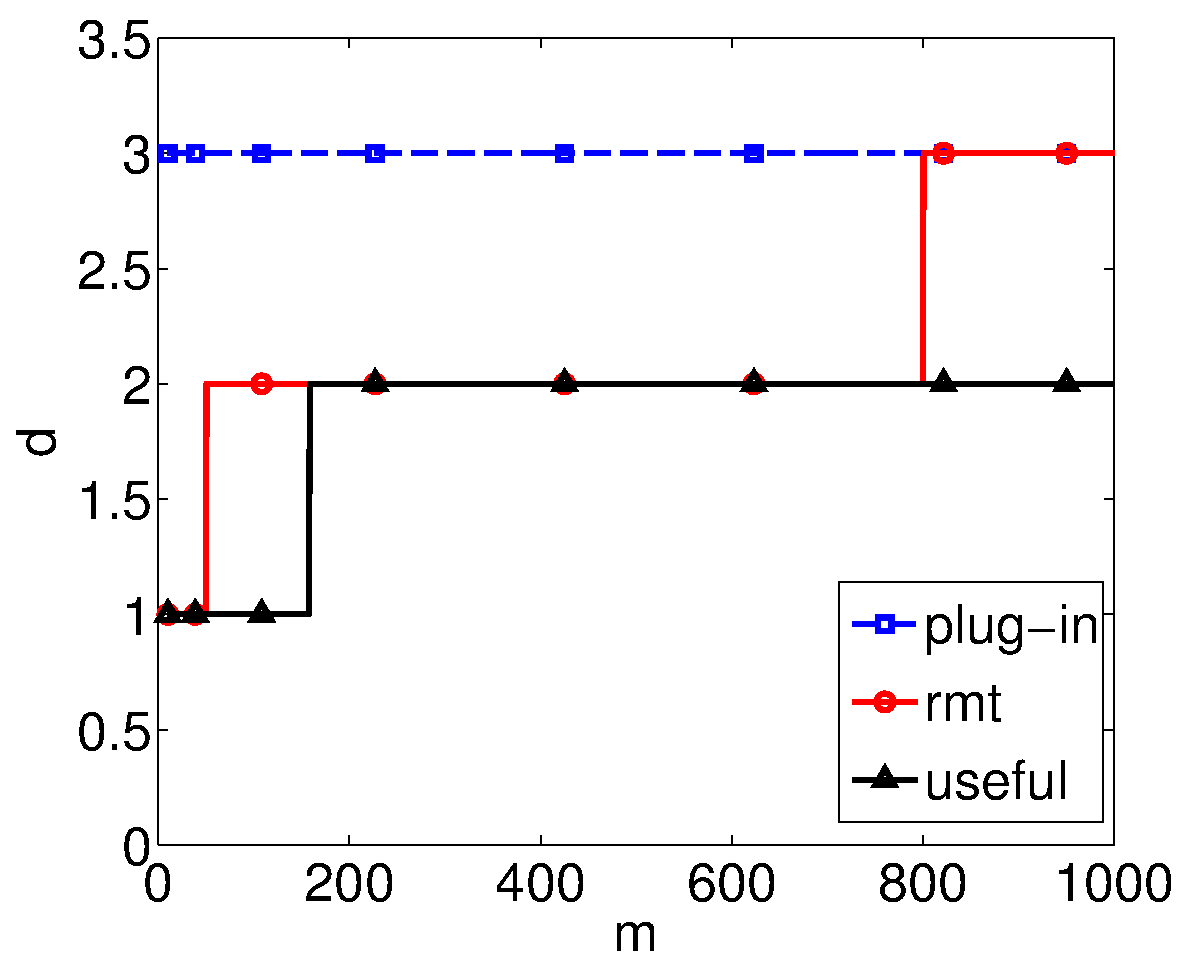
\includegraphics[width=0.45\textwidth]{taes_msd/figures/taes_d_v_m.pdf}
  \label{fig:dvals}}
\caption{Deterministic energy detector performance as a function of the number of training
  samples. In this experiment $n=200$, $\Sigma =\diag(5,2,0.5)$, $x=[1.5,1.5,1.5]^T$, and
  the required false alarm rate is $P_F=0.1$. (a) The theoretical probability of detection
  achieved by the plug-in, RMT, and useful detectors. $P_D(P_F)$ is calculated in
  (\ref{eq:roc}). The plug-in detector sets $d=k$, the RMT detector sets $k=\keff$ as
  defined in (\ref{eq:keff}), and the useful detector sets $d=\kuse$ as calculated in
  Figure \ref{algo:kuse} using the non-centrality parameter defined in
  (\ref{eq:msd_nc_param}). The useful detector achieves the optimal performance. (b) The
  number of subspace components used by the plug-in, RMT, and useful detectors. Whenever
  $\keff\neq\kuse$, the RMT detector realizes a suboptimal detector performance. Even
  though these subspace components are \textit{informative}, there is not enough training
  data to make them \textit{useful} in detection.}
\label{fig:main_result}
\end{figure}

Evident in Figure \ref{fig:det_perf}, the detector using $\kuse$ subspace components
achieves the maximum detection ability of all detectors for every amount of training
samples. This is slightly contrived because $\kuse$ is optimized to do just this. More
importantly, we empirically see that using $\keff$ subspace components is not always
optimal.  However, examination of Figure \ref{fig:dvals} reveals why this occurs. For
$50\leq m\leq 160$, $\keff=2>\kuse=1$. Therefore, even though the second subspace
component is informative by definition, it is not \textit{useful} in detection. Including
it in an energy detector decreases detector performance. A similar phenomenon
occurs at $m=800$ when $\keff$ increases to 3 but $\kuse$ remains constant at 2. Unlike
the RMT detector, the detection performance of the useful detector increases monotonically
with an increase in training samples. Both the RMT and useful detectors outperform the
standard plug-in detector which uses all $k$ subspace components.


\section{Extension - Weighted Energy Detector}\label{sec:ext}
The energy detector in (\ref{eq:energy_detector}) may be generalized by adding a
non-negative weight to each component in the sum. The statistic for the
weighted energy detector is 
\beq\label{eq:weighted_detector}
\Lambda_{\text{weighted}}(w) = w^TAw = \sum_{i=1}^k a_iw_i^2.
\eeq
where $A=\diag(a_1,\dots,a_k)\in\reals^{k\times k}$ and $a_i\geq0$. We constrain $\sum_{i=1}^k a_i = 1$ so that the weights
reside on the $(k-1)$-simplex. This reduces the set of possible weights by eliminating
those that are multiples of each other, which results in equivalent
detectors. The weighted energy detector gives practitioners additional design freedom to
maximize detector performance. Using a similar analysis as in Section
\ref{sec:energy_detector}, the conditional distributions of the weighted energy detector's 
statistic in (\ref{eq:weighted_detector}) are
\beq\label{eq:roc_weighted}
\ba
&\Lambda(w)|H_0\sim\sum_{i=1}^k a_i\chi_{1i}^2,\\
&\Lambda(w)|H_1\sim\sum_{i=1}^k a_i \chi_{1i}^2\left(\delta_i^2\right),
\ea
\eeq
where $\chi_{1i}^2$ are independent chi-square random variables with one degree of freedom
and $\chi_{1i}^2\left(\delta_i^2\right)$ are independent non-central chi-square random variable
with one degree of freedom and non-centrality parameter $\delta_i^2$. We can relate $P_D$
to $P_F$ using the expression
\beq\label{eq:weighted_pd}
P_{D_{\text{weighted}}}(P_F,A) = 1 - Q_{\Lambda|H_1}\left(Q^{-1}_{\Lambda|H_0}(1-P_F)\right)
\eeq
where $Q_{\Lambda|H_1}$ is the c.d.f of $\Lambda(w)|H_1$ in (\ref{eq:roc_weighted})
and $Q_{\Lambda|H_0}$ is the c.d.f. of $\Lambda(w)|H_0$ in (\ref{eq:roc_weighted}). 

The definition of $\Lambda_{\text{weighted}}(w)$ in (\ref{eq:weighted_detector}) raises
the natural question 
\begin{quote}
  Given $\delta$ and a desired $P_F$, what is the optimal choice of weighting matrix, $A$,
  that maximizes $P_{D_{\text{weighted}}}(P_F)$ for a weighted energy detector with the
  form of (\ref{eq:weighted_detector}) using observations generated from
  (\ref{eq:general_setup})?
\end{quote}
While the c.d.f. of chi-square and non-central chi-square random variables are known in
closed form, the c.d.f. of a weighted sum of chi-square random variables is not known in closed
form and therefore (\ref{eq:weighted_pd}) cannot be computed analytically. It is common
to use saddlepoint approximation techniques \cite{wood1993saddlepoint} to compute the
c.d.f. of such sums in (\ref{eq:roc_weighted}), however, such techniques must be computed
for many thresholds, $\eta$, to generate a ROC curve for one weighting matrix $A$. To
optimize over $A$ in (\ref{eq:weighted_pd}), this process would need to be repeated over a
discretization of the ($k-1$)-simplex. Developing a more efficient algorithm to optimize
over the weighting matrix, $A$, is an important topic for future work.

To illustrate how weighted energy detectors can improve detection performance, consider a rank-2 setting where the desired
false alarm rate is $P_F=0.1$. Optimizing $A=\diag(a_1,a_2)$ on the simplex $a_1+a_2=1$
results in one degree of freedom and so
\be
\Lambda(w)_{\text{weighted}} = aw_1^2 + (1-a)w_2^2  
\ee
where $a\in[0,1]$. Figure \ref{fig:weighted} plots the empirically achieved (see
\cite{fawcett2006introduction}) probability of detection as a 
function of the weighting parameter $a$ for four detectors each with a different signal
vector $\delta$. Figure \ref{fig:weights_easy} shows results for detectors using
$\delta=[1,1]^T$ and $\delta=[1,0]^T$. The detector with $\delta=[1, 1]^T$ achieves
maximum performance when $a=0.5$, which weights both components equally. As
$\delta_1=\delta_2=1$ both $w_1$ and $w_2$ have the same conditional distributions and it
is intuitive that we weight both components equally. However, the detector using
$\delta=[1, 0]^T$ achieves maximum performance when $a=1$ indicating that the second
component is not useful in detection. As $\delta_2=0$, $w_2$ has the same distribution
under both the $H_1$ and $H_0$ hypotheses, giving it no discriminatory power. For these
values of $\delta$, the optimal $a$ is obvious and the performance of the weighted energy
detector is the same as that of the standard energy detector.

\begin{figure}[t]
\centering
\subfigure[Easy Optimal Weights]{
  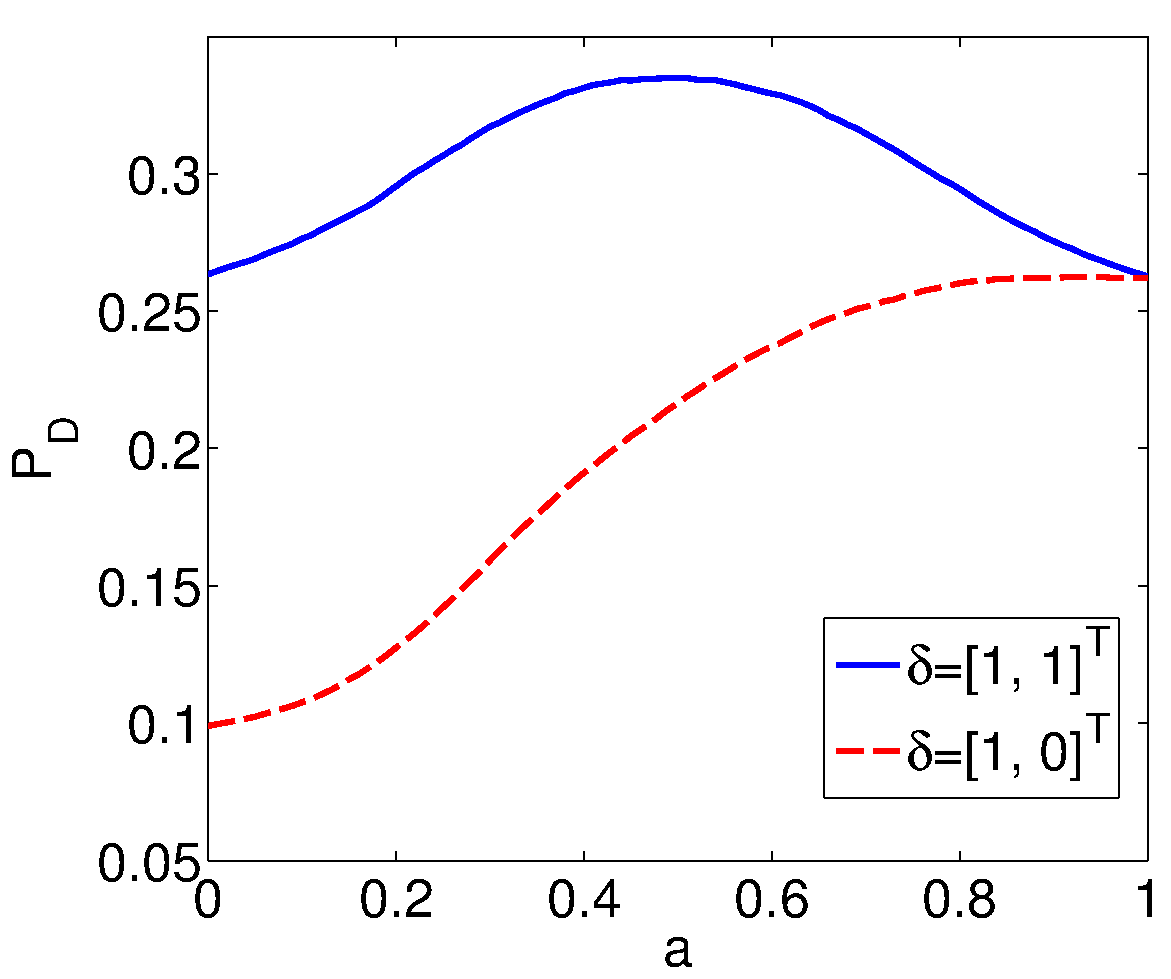
\includegraphics[width=0.45\textwidth]{taes_msd/figures/weights_easy.pdf}
  \label{fig:weights_easy}}
\subfigure[Difficult Optimal Weights]{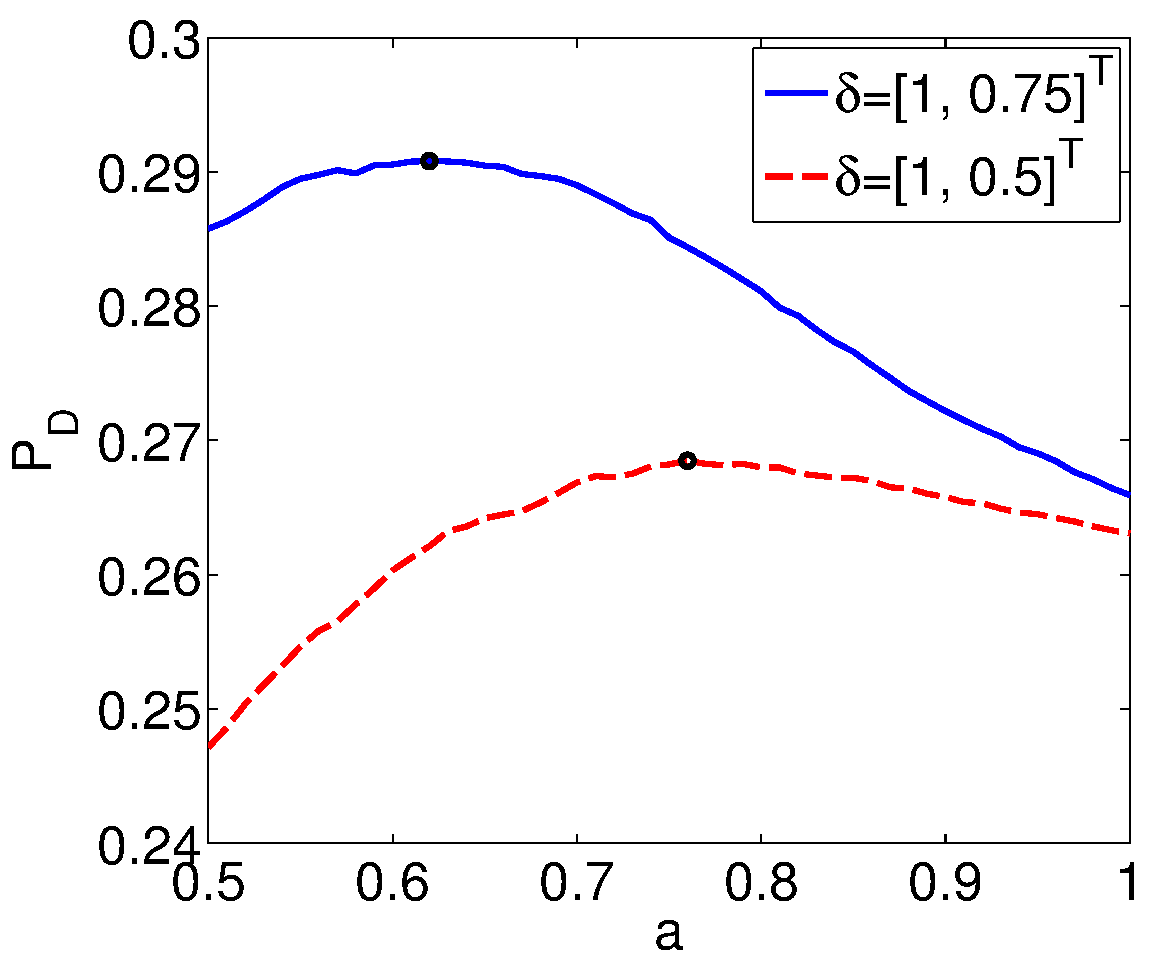
\includegraphics[width=0.45\textwidth]{taes_msd/figures/weights_hard.pdf}
  \label{fig:weights_hard}}
\caption{Empirically achieved probability of detection ($P_D$) as a function of the
  weighting coefficient $a$ for a fixed false alarm rate of $P_F=0.1$. (a) Two detectors,
  one using the deterministic vector $\delta=[1,1]^T$ and the second using
  $\delta=[1,0]^T$.  The first detector achieves its maximum performance around $a=0.5$
  indicating that both components are equally informative. The second detector achieves
  its maximum performance at $a=1$ indicating the second subspace component is not useful
  in detection. (b) Two detectors, one using $\delta=[1, 0.75]^T$ and the other using
  $\delta=[1, 0.5]^T$. The maximum performance of each detector is no longer achieved at
  $a=0.5$ or $a=1$ as the entries of $\delta$ are non-zero and are not equal. The maximum
  performance is indicated by a black circle.}
\label{fig:weighted}
\end{figure}


Figure \ref{fig:weights_hard} considers detectors using $\delta=[1, 0.75]^T$ and $\delta=[1,
0.5]^T$. Both choices place $\delta_1>\delta_2$ so we only consider the regime $a\in[0.5,
1]$, which weights the first component stronger than the second. The maximum performance
of each detector is indicated by a black circle. Unlike the detectors in Figure
\ref{fig:weights_easy}, the maximum $P_D$ is not achieved at $a=0.5$ or $a=1$; both
components are needed to achieve optimal performance. For these choices of $\delta$, the
weighted energy detector is able to achieve a better performance than a standard energy
detector using either one ($a=1$) or both ($a=0.5$) components. Developing an efficient algorithm
to compute these optimal weights is an important extension of the work in this chapter.


%\section{Extension to Missing Data}\label{sec:chpt3:missing}
%\begin{abstract}
%We consider a matched subspace detection problem where a signal vector residing in an unknown low-rank $k$ subspace is to be detected using a subspace estimate obtained from noisy signal-bearing training data with missing entries. The resulting subspace estimate is inaccurate due to limited training data, missing entries, and additive noise. Recent results from random matrix theory (RMT) precisely quantify these subspace estimation errors for the setting where the signal has low coherence. We analytically quantify the ROC performance of the resulting plug-in detector and derive a new detector which explicitly accounts for these subspace estimation errors. The realized increase in performance can be attributed to the new detector only using the $k_\text{eff}\leq k$ ``informative'' signal subspace components. The fraction of observed entries determines $k_\text{eff}$ via a simple relationship that we describe. Detection performance better than random guessing is only achievable when the percent of observed data is above a critical threshold which we explicitly characterize.
%\end{abstract}
%

%\section{Introduction}\label{sec:intro}

%The matched subspace detector (MSD) is a widely used tool in signal processing and machine learning to detect a signal embedded in a low-rank subspace in the presence of additive noise \cite{scharf1994matched,jin2005cfar,mcwhorter2003matched}. The performance of the MSD has been explored when the low-rank signal subspace is known. Scharf and Friedlander \cite{scharf1994matched} consider the MSD when the signal is placed deterministically at an unknown location in a known subspace while McWhorter and Scharf \cite{mcwhorter2003matched} extend this work to allow the signal to be placed randomly with a known (or assumed) distribution in the known subspace.

%There is little work characterizing the performance of the matched subspace detector when the signal subspace is unknown and estimated from data. Recently, we used RMT to quantify the performance of stochastic MSDs in such a setting  \cite{asendorf2011msd}. That work brought into sharp focus the importance of using $k_\text{eff}\leq k$ informative signal subspace components in detector statistics; here $k_{\text{eff}}$ is the effective number of informative components identifiable from limited, noisy data as described in \cite{nadakuditi2008sample}. In this paper, we extend the analysis to the deterministic MSD setting where the training data is noisy \textit{and} has missing entries. The missing entry context is motivated in \cite{balzano2010high} by distributed detection scenarios where it might be prohibitive to collect and transmit only a (randomly chosen) fraction $p$ of the training data entries. Alternately one might think of $1-p \in (0,1)$ as a compression factor as in compressed sensing.

%The main contribution of this paper is a precise quantification of the resulting performance of the MSD. We uncover a phase transition phenomenon by showing that there is a critical fraction, $p_\text{crit}$, which is a simple function of the eigen-SNR, the number of training samples, and the number of sensors, below which detection performance deteriorates to random guessing. Compressing the training dataset below this critical fraction is undesirable.

%The paper is organized as follows. Section \ref{sec:prob stat} formally states the detection problem. Section \ref{sec:rmt} presents pertinent results from RMT. These results are used in Section \ref{sec:derive} to derive a plug-in and random matrix theory MSD and in Section \ref{sec:roc} to derive theoretical ROC curves for each detector. Section \ref{sec:results} validates our analytical predictions, highlights the importance of selecting $k_\text{eff}$ over $k$ subspace components, and demonstrates the effect of missing data. Section \ref{sec:conclusion} presents concluding remarks.

\section{Deterministic Matched Subspace Detectors with Missing Data}\label{sec:chpt3:missing}

We consider the same detection setting as described in Section \ref{sec:msd} using the training
data model in (\ref{eq:taes_train}). However, we only observe a
fraction $p\in(0,1)$ of the entries of our training matrix $Y=[y_1,\dots,y_m]$; $p$ is
independent of $n$ and $m$. Define our observed training data matrix, $\widetilde{Y}$, as
\beq\label{eq:data_model_miss}
\widetilde{Y} = Y\odot M
\eeq
where
\be
 M_{ij} = \begin{cases} 1 & \text{ with probability } \gamma_y\\ 0 & \text{ with
    probability } 1-\gamma_y \end{cases}
\ee
and $\odot$ denotes the Hadamard or element-wise product. Finally we make the following
assumption about our signal subspace, $U$.

\begin{Assum}\label{assum:msd_coher}
In the missing data setting, assume that the columns of $U$ satisfy a `low-coherence'
condition in the following sense: we suppose that there exist 
non-negative constants $\eta$, $C$ independent of $n$, such that for $i=1,\dots,k$ 
\be
\max_i \|u_i\|_\infty \leq \eta\frac{\log^{C}n}{\sqrt{n}}.
\ee
\end{Assum}
We form a signal subspace estimate as in (\ref{eq:param_estims_stoch}), except that we use
our partially observed training matrix $\widetilde{Y}$ to form the sample covariance
matrix $S$ . Call this signal subspace estimate $\widetilde{U}$. 

\subsection{Pertinent Results from RMT}\label{sec:rmt}

By modifying an argument in  \cite{benaych2011singular}, we obtain the following result.
\begin{Th}\label{th:angles}
Assume that $x_i \sim \mathcal{CN}(0,\Sigma^2)$ as in (\ref{eq:taes_train}) and that $U$
in (\ref{eq:taes_train}) obeys the low coherence condition in Assumption
\ref{assum:msd_coher}. Then as $n,m \to \infty$ with $n/m \to c$ we have that
for $i,j = 1, \ldots, k$: 
\begin{equation*}
\begin{aligned}
&|\langle u_i,\widehat{u}_i\rangle|^2\convas
\begin{cases}
1-\dfrac{c\left(1+p\sigma_i^2\right)}{p\sigma_i^2\left(p\sigma_i^2 + c\right)} & \text{ if } \sigma_{i}>\dfrac{c^{1/4}}{\sqrt{p}}\\
0 & \textrm{otherwise}\\
\end{cases}\\
&|\langle u_i,\widehat{u}_j\rangle|^2\convas 0 \qquad \textrm{ for } i \neq j.\\
\end{aligned}.
\end{equation*}
where $\widehat{u}_i$ are the left singular vectors of $\widetilde{Y}$.
\end{Th}

The low coherence condition appears in, for example, \cite{balzano2010high} with the idea
being that the matrix $U \begin{bmatrix} x_{1} & \ldots & x_{m} \end{bmatrix}$ has entries
of about the same magnitude. With the Gaussianity assumption for $x$, all we need is $U$
to have low coherence. Recall that the coherence of a matrix with orthonormal columns is
$\max_{i,j}|U_{i,j}|$. When a matrix is spiky, random sampling of its entries may result
in a loss of information; matrices with low coherence behave better under random sampling
and it is this setting that we focus on in this chapter.

The key insight from Theorem \ref{th:angles} is that only the singular vectors
corresponding to signal singular values above the phase transition
$\frac{c^{1/4}}{\sqrt{p}}$ are \textit{informative}. The fraction of missing entries $p$
regulates this phase transition point as $O(1/\sqrt{p})$. When a signal singular value
drops below this critical threshold, the corresponding singular vector estimate is
essentially noise-like (i.e. $|\langle u_i,\widehat{u}_i\rangle|^2=o_{p}(1)$) and thus
\textit{uninformative}. The term $|\langle u_i,\widehat{u}_i\rangle|^2$ quantifies
mismatch between the estimated and underlying singular vectors; when $p < p_{\text{crit.}}
:=\sqrt{c}/\max_{i}(\sigma_{i}^{2})$ then \textit{all} singular vectors are
uninformative. Intuitively we expect a degradation in the performance of detectors that
utilize subspace components for which $|\langle u_i,\widehat{u}_i\rangle|^2=o_{p}(1)$.  We
refer to the estimate in Theorem \ref{th:angles} as $|\langle
u_i,\widehat{u}_i\rangle|^2_{\text{rmt}}$.

\subsection{Plug-in and RMT Detectors}\label{se:miss_detects}

Using the estimate of our signal subspace, $\widetilde{U}$, formed from our partially
observed training data matrix $\widetilde{Y}$, we define 
\be
\widetilde{w} = \widetilde{U}^Ty
\ee
where $y$ is a testing vector from (\ref{eq:determ_setup}). Note that in this setup, we
don't assume that our testing observation has any missing entries. Following a similar
derivation from Chapter 2 and the previous section, we have our plug-in and RMT test
statistics are
\begin{equation}\label{eq:plugin missing}
\Lambda_{\text{plugin}}(\widetilde{w}) =\widetilde{w}^H\widetilde{w}\sum_{i=1}^k\widetilde{w}_i^2
\end{equation}
\begin{equation}\label{eq:rmt_missing}
\Lambda_{\text{plugin}}(\widetilde{w}) =\widetilde{w}^H\widetilde{w}\sum_{i=1}^{\keff}\widetilde{w}_i^2
\end{equation}
where we define $k_\text{eff}$ as the number of signal singular values above the phase
transition $\frac{c^{1/4}}{\sqrt{p}}$ shown in Theorem \ref{th:angles}. We may use either
test statistic to form a detector of the form 
\begin{equation}\label{eq:opt classifier}
\Lambda(\widetilde{w}) \detgtrless \ln(\eta)
\end{equation}
where $\eta$ satisfies $P(\Lambda(\widetilde{w})>\ln\left(\eta\right)|H_0)=\alpha$.

\subsection{Theoretical ROC Curve Derivation}\label{sec:roc_missing}
A standard way to compare the plug-in and RMT detectors derived in (\ref{eq:plugin missing}) and (\ref{eq:rmt_missing}) respectively is to compute their ROC curves. For a particular statistic $\Lambda(\widetilde{w})$, to compute theoretical ROC curves, we must compute
\begin{equation}\label{eq:target cdf}
\begin{aligned}
&P_D = P(\Lambda(w) > \gamma| w\in H_1)\\
&P_F = P(\Lambda(w) > \gamma| w\in H_0)\\
\end{aligned}
\end{equation}
for $-\infty<\gamma<\infty$. To do this, we explore the conditional CDF under each hypothesis for the statistics (\ref{eq:plugin missing}) and (\ref{eq:rmt_missing}).

This derivation is the same as in Chapter 2 except that we replace $|\langle
u_i,\widehat{u}_i\rangle|_{\text{rmt}}^2$ with the expression in Theorem \ref{th:angles}. 

\section{Simulation Results and Discussion}\label{sec:results}

\begin{figure}[t]
\centering
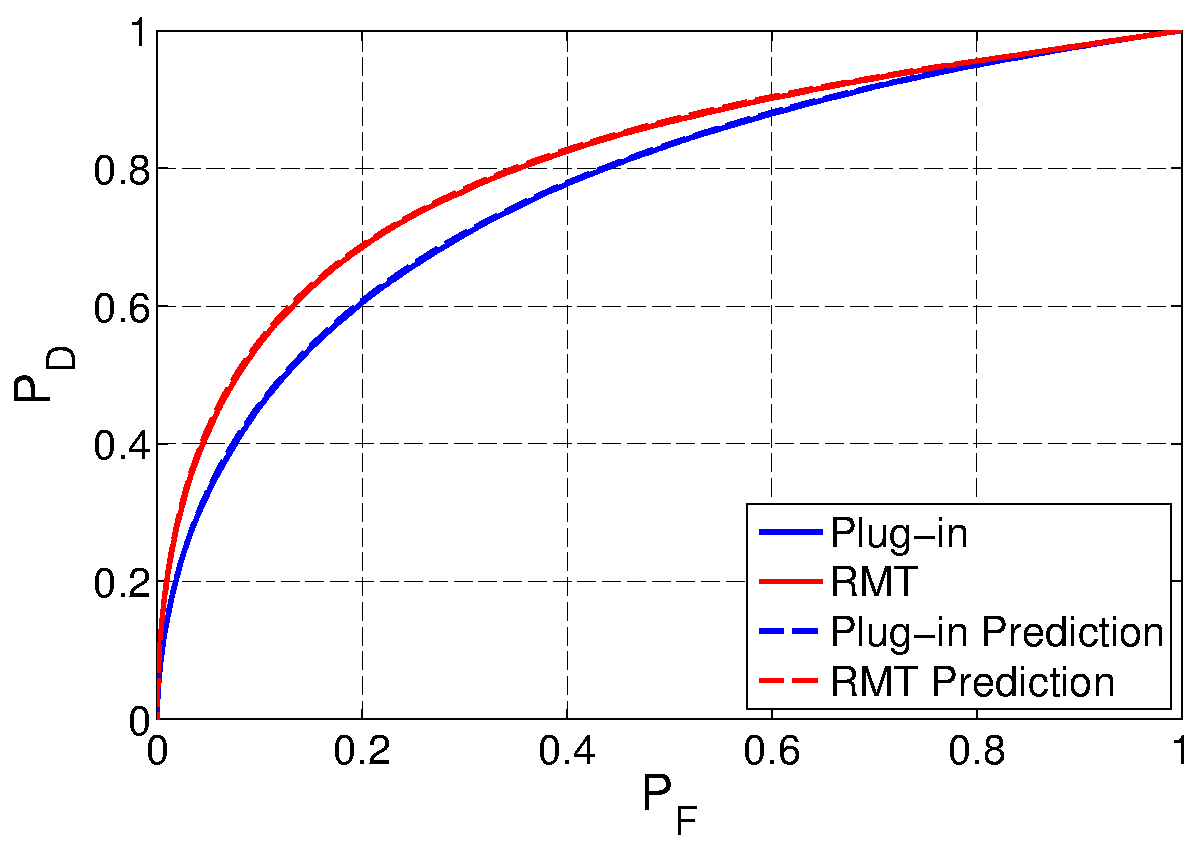
\includegraphics[width=3in]{msd_missing/figures/basic_roc.pdf}
\caption{Empirical and theoretical ROC curves for the plug-in and RMT matched subspace detectors. Empirical ROC curves were simulated with $n=500$, $m=500$, $k=2$, $\Sigma=\diag(3,0.1)$, and $p=0.8$. However, as $\sigma_2$ is below the critical threshold, $k_{\text{eff}} = 1$. The empirical ROC curves were computed using $5000$ test samples and averaged over 25 trials. $x$ was generated randomly for training samples but fixed for test samples. The theoretical ROC curves were obtained using (\ref{eq:roc}). Note the excellent agreement and the performance gain realized by the RMT detector.}\vskip-0.45cm
\label{fig:roc1}
\end{figure}


\subsection{ROC Curves}

We consider a setting where $k_{\text{eff}} = 1 < k = 2$. For this setting, as seen in Figure \ref{fig:roc1}, for any false alarm rate ($P_F$), the RMT detector achieves a higher probability of detection ($P_D$), demonstrating the sub-optimality of the plug-in detector. This is expected because $k_\text{eff}<k$ so that the plug-in detector is employing uninformative subspace components. The theoretical ROC curves in (\ref{eq:roc}) match the empirically generated ROC curves validating the performance predictions of (\ref{eq:roc}) which rely on Theorem \ref{th:angles}.

\subsection{Effect of Missing Data}
Figure \ref{fig:sparsity} examines the performance of each detector as a function of $p$. Again we observe the sub-optimality of the plug-in detector. The theoretical $P_D$ prediction in (\ref{eq:roc}) matches empirically achieved $P_D$ for both detectors. As expected, as $p$ decreases, the achieved probability of detection decreases. We note the presence of a critical $p_{\text{crit.}} : = \sqrt{c}/\max_{i}(\sigma_{i}^{2})$ obtained from Theorem \ref{th:angles}, below which (in the large system limit) we may only achieve $P_D=P_F$; the rounding in Figure \ref{fig:sparsity} is attributed to finite system approximation error.

\begin{figure}[t]
\centering
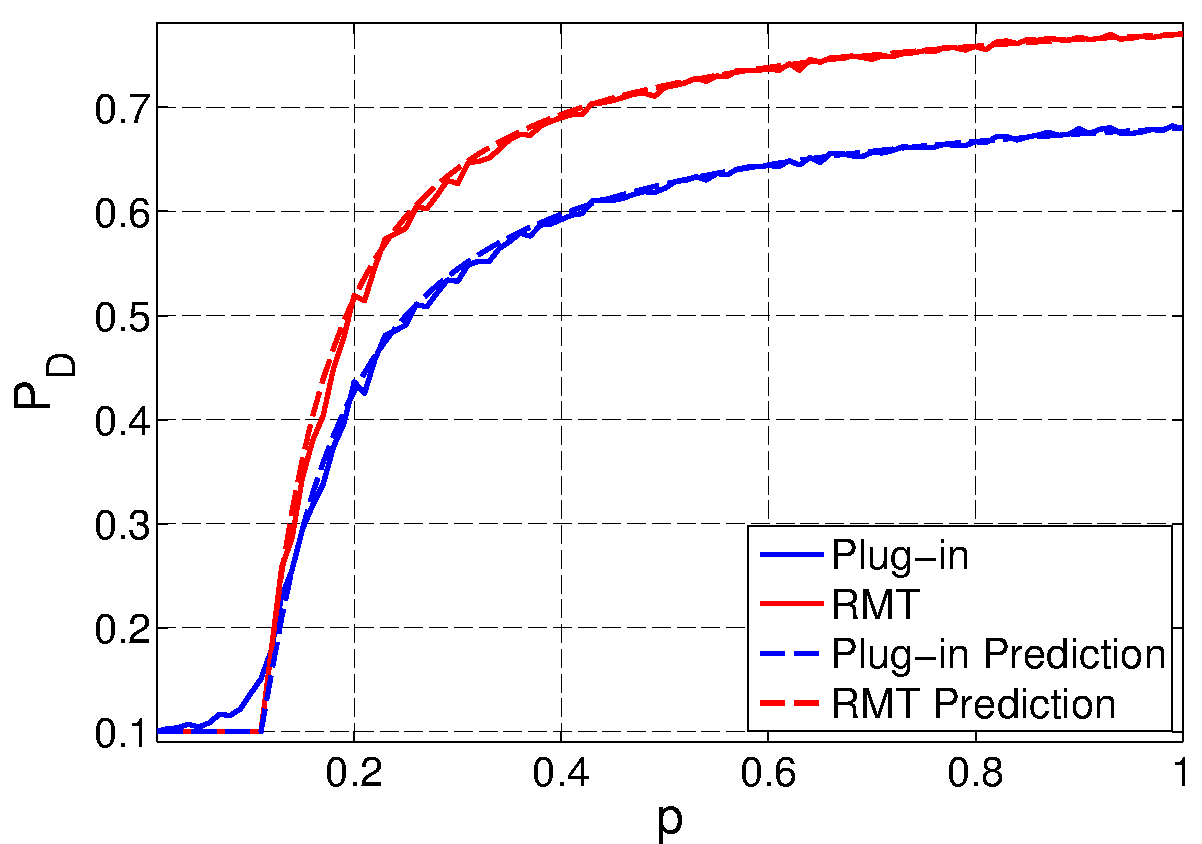
\includegraphics[width=3in]{msd_missing/figures/sparsity.pdf}
\caption{Empirically computed probability of detection, $P_D$, for a fixed probability of false alarm, $P_F=0.1$, for various $p$. Here, $n=1000$, $m=1000$, $k=2$, $\Sigma=\diag(3,0.1)$. $P_D$ was computed using (\ref{eq:roc}) and $x$ was generated as described in Figure \ref{fig:roc1}. For values of $p \leq 1/9$, $k_\text{eff}=0$ and performance degrades to $P_D = P_F +o(1)$ for both detectors. As $p$ increases, $k_\text{eff}=1$ allowing the detectors to achieve better than random guessing performance. When $k_\text{eff}>0$ the plug-in detector is sub-optimal for all values of $p$.}\vskip-0.45cm
\label{fig:sparsity}
\end{figure}





\section{Conclusion}\label{sec:conclusion}
In this paper, we considered a matched subspace detection problem where the low-rank signal subspace is unknown and must be estimated from finite, noisy, signal-bearing training data. We considered both a stochastic and deterministic model for the testing data. The subspace estimate is inaccurate due to finite and noisy training samples and therefore degrades the performance of plug-in detectors compared to an oracle detector. We showed how the ROC performance curve can be derived from the RMT-aided quantification of the subspace estimation accuracy.

Armed with this RMT knowledge, we derived a new RMT detector that only uses the effective number of informative subspace components, $k_\text{eff}$. Plug-in detectors that use the uninformative components will thus incur a performance degradation, relative to the RMT detector. \textcolor{blue}{In settings where a practitioner might play-it-safe and set $\widehat{k}> \widehat{k}_{\text{eff}}$, the performance loss in significant (see Figures \ref{fig:stoch_theory_epsilon} and \ref{fig:determ_theory_epsilon} for a demonstration of how much training data such a play-it-safe plug-in detector would need to match the performance of a $\keff$-tuned RMT detector).} This highlights the importance of robust techniques \cite{nadakuditi2010fundamental,johnstone2001distribution,el2007tracy} for estimating $k_\text{eff}$ in subspace based detection schemes as opposed to estimating $k$, particularly in the regime where $k_{\text{eff}} < k$.  We showed in Tables \ref{table:summary_stoch} and \ref{table:summary_determ} that the distributions of the test statistics could be expressed as a weighted sum of independent chi-squared random variables. The associated ROC curves can then be computed using a saddlepoint approximation.

\textcolor{blue}{The results in this paper can be extended in several directions. We note that the stochastic detector setting assumed normally distributed training and test data. We can extend the analysis to the Gaussian training data but non-Gaussian test vector setting by `integrating-out' the deterministic detector performance curves with respect to the non-Gaussian distribution of the test-vector. Our results relied on characterization of the quantity $\langle u_{j},\widehat{u}_{i}\rangle$.  Thus analogous performance curves can be obtained for any alternate training data models for which this quantity can be analytically quantified. To that end, the results in \cite{benaych2011singular} facilitate such an analysis for a broader class of models including the correlatted Gaussians training data setting. An extension to the missing data setting might follow a similar approach and appears within reach. Aspects related to rate of convergence are open and will be the subject of future work.}



%\bibliographystyle{IEEEtran}
%\bibliography{IEEEabrv,taes_useful.bib}


\chapter{Background: Canonical Correlation Analysis (CCA)}\label{sec:cca}
We begin by providing an overview of canonical correlation analysis (CCA). For
completeness and ease of future derivations, we derive the solution for CCA from first
principles. We then give an overview of previous work on CCA in the sample starved regime,
summarizing the results of \cite{pezeshki2004empirical,nadakuditi2011fundamental}. We
conclude by providing new results based on the observations in
\cite{nadakuditi2011fundamental}.

\section{Mathematical Formulation of CCA}\label{sec:cca_form}
Assume that observations $\yI\in\complex^{d_1}$, $\yII\in\complex^{d_2}$
are drawn from two distributions $\yI\sim\mathcal{Y}_1$,
$\yII\sim\mathcal{Y}_2$. Furthermore, assume that the distributions have zero mean,
\textit{i.e.} $\E{\yI}=\E{\yII}=0$. We will use the following notation for the covariance
matrices of the distributions: $\E{\yI\yI^H}=\RI$, $\E{\yII\yII^H}=\RII$,
$\E{\yI\yII^H}=\RIII$.

The goal of CCA is to find a linear transformation for each dataset that maximizes the
correlation between the datasets in the projected spaces. We represent the linear
transformations with the canonical vectors $\xI\in\complex^{d_1}$ and
$\xII\in\complex^{d_2}$ and the projection with the canonical variates $\wI=\xI^H\yI$ and
$\wII=\xII^H\yII$. The objective is to find the canonical vectors $\xI$ and $\xII$ that
maximize the correlation between the canonical variates $\wI$ and $\wII$. Formally, the
optimization problem is
\begin{equation}\label{eq:cca_opt}
  \begin{aligned}
    &\argmax_{\xI,\xII}&&\rho = \E{\wI\wII}\\
    & \text{subject to}&&\E{\wI^2}=1, \E{\wII^2}=1.
  \end{aligned}
\end{equation}
Substituting the expressions for the canonical variates and the correlation matrices, this
optimization problem may be written as
\begin{equation}\label{eq:cca_opt2}
  \begin{aligned}
    &\argmax_{\xI,\xII}&&\rho = \xI^H\RIII\xII\\
    & \text{subject to}&&\xI^H\RI\xI=1, \xII^H\RII\xII=1.
  \end{aligned}
\end{equation}

The Lagrangian used to solve (\ref{eq:cca_opt2}) is
\begin{equation}\label{eq:cca_lagr}
  L(\xI,\xII,\lambda_1,\lambda_2) = \xI^H\RIII\xII - \lambda_1(\xI^H\RI\xI -1) - \lambda_2(\xII^H\RII\xII-1).
\end{equation}
Solving (\ref{eq:cca_opt2}) is achieved by setting the partial derivatives of
(\ref{eq:cca_lagr}) equal to zero. Doing so yields 
\beq\label{eq:cca_partials}\ba
& 0 && = \RIII\xII -2\lambda_1\RI\xI\\
& 0 && = \RIII^H\xI -2\lambda_2\RII\xII.\\
\ea\eeq 
By left multiplying the first equation of (\ref{eq:cca_partials})by $\xI^H$ and
the second equation by $\xII^H$ and using the definitions and constraints in
(\ref{eq:cca_opt2}), 
\beq\label{eq:cca_rho} 
\rho = 2\lambda_1=2\lambda_2.
\eeq 
Therefore, the Lagrange multipliers are equal and the value of the maximum correlation
between the datasets is a multiple of the Lagrange multiplier. Solving one equation in
(\ref{eq:cca_partials}) for $\xII$ and substituting in the other results in the following
eigenvalue system
\cite{nielsen2002multiset,nadakuditi2011fundamental,welling2005kcca,kettenring1971canonical,nielsen1994analysis}
\begin{equation}\label{eq:cca_eigval_sys}
  \RI^{-1}\RIII\RII^{-1}\RIII^H\,\xI = \rho^2\xI
\end{equation}
with the relationship
\beq\label{eq:x2}
\xII=\frac{1}{\rho}\RII^{-1}\RIII^H\,\xI.
\eeq

Solving (\ref{eq:cca_eigval_sys}) for the eigenvector corresponding to the largest
eigenvalue solves (\ref{eq:cca_opt2}). Substituting this eigenvalue/eigenvector pair in
(\ref{eq:x2}) gives the complete solution $\left(\xI,\xII,\rho\right)$ for the transformations
  and maximum correlation between the datasets. Multiple canonical basis vectors may be
  found by recursively finding the next largest eigenvalue and corresponding eigenvector
  in (\ref{eq:cca_eigval_sys}). In many learning applications, it is common to project
  onto multiple canonical basis vectors.

 Using a similarity transform, we can frame the eigen-system in (\ref{eq:cca_eigval_sys})
 as an SVD problem. Define $f = \RI^{1/2}\xI$ and $g=\RII^{1/2}\xII$. Then
 (\ref{eq:cca_eigval_sys}) may be rewritten as
\begin{equation}\label{eq:eigval_sys2}
  \RI^{-1/2}\RIII\RII^{-1}\RIII^H\RI^{-H/2}f = \rho^2f.
\end{equation}
Defining $C=\RI^{-1/2}\RIII\RII^{-H/2}$, (\ref{eq:eigval_sys2}) can be rewritten as
\begin{equation}\label{eq:cca_C_eigval}
  CC^Hf=\rho^2f.
\end{equation}

Clearly, from (\ref{eq:cca_C_eigval}), we may obtain a closed form solution for $f$ and
$\rho$ through the SVD of $C$. Let $FKG^H$ be the SVD of $C$ where
$F=[f_1,\dots,f_{d_1}]$, $K\in\complex^{d_1\times
  d_2}=\diag(k_1,\dots,k_{\min\left(d_1,d_2\right)})$, and $G=[g_1,\dots,g_{d_2}]$. Then the solution
for the canonical vector pair corresponding to the largest canonical correlation is
\beq\label{eq:cca_svd_sol}\ba
&\rho = k_1\\
&\xI = \RI^{-1/2}f_1\\
&\xII = \RII^{-1/2}g_1.\\
\ea\eeq

\section{Empirical CCA}\label{sec:emp_cca}

The above analysis assumes that the covariance matrices $\RI$, $\RII$, and $\RIII$ are all
known. However, in most applications these covariance matrices are unknown and must be
estimated from data. In such an empirical setting, we assume that we are given $n$
observations, or samples, from each dataset $\yI^{(i)}$ and $\yII^{(i)}$ for
$i=1,\dots,n$. We may stack these observations in training data matrices
\be
Y_1=\left[\yI^{(1)},\dots,\yI^{(n)}\right], \text{ and } 
Y_2=\left[\yII^{(1)},\dots,\yII^{(n)}\right].
\ee
Using these training data matrices, the sample covariance matrices are
\beq\label{eq:scm}\ba
&\RIhat = \frac{1}{n} Y_1Y_1^H\\
&\RIIhat = \frac{1}{n} Y_2Y_2^H\\
&\RIIIhat = \frac{1}{n} Y_1Y_2^H.\\
\ea\eeq
We may then substitute these covariance matrix estimates in the expression for $C$,
resulting in the estimator
\beq\label{eq:cca_Chat}
\widehat{C} = \RIhat^{-1/2}\RIIIhat\RIIhat^{-1/2}.
\eeq
Defining $\widehat{C} =\widehat{F}\widehat{K}\widehat{G}^H$ as the SVD of $\widehat{C}$,
the solution to empirical CCA is
\beq\label{eq:cca_svd_sol}\ba
&\widehat{\rho} = \widehat{k}_1\\
&\xIhat = \RIhat^{-1/2}\,\widehat{f}_1\\
&\xIIhat = \RIIhat^{-1/2}\,\widehat{g}_1.\\
\ea\eeq

\section{Performance of Empirical CCA}

Here, we present the relevant works that explore the performance of empirical CCA and
demonstrate how they provide insight to the data fusion questions posed herein. First, we
note that to construct $\widehat{C}$ in (\ref{eq:cca_Chat}) we must invert $\RIhat$ and
$\RIIhat$. However, if the number of samples $n$ is less than either of the data
dimensions $d_1$ or $d_2$, then the sample covariances are not invertible. In this case, a
regularized version of CCA is often employed. We discuss this in depth in Chapter
\ref{sec:rcca}.

\subsection{Performance Breakdown When $n<d_1+d_2$}
Pezeshki et al. analyze the performance of empirical CCA in the sample poor regime when
$n<d_1+d_2$ in \cite{pezeshki2004empirical}. In particular, they show that in this regime,
empirical CCA breaks down completely; the leading singular value of $\widehat{C}$ is 
deterministically 1. Below we provide a different proof of this result.

Let $Y_1 = U_1\Sigma_1 V_1^H$ and $Y_2=U_2\Sigma_2V_2^H$ be the data SVDs of our training
data matrix. Using this notation, 
\beq\label{eq:cca_chat_svd}\ba
& \widehat{C} &&= \RIhat^{-1/2}\RIIIhat\RIIhat^{-1/2}\\
&&&  = \left(Y_1Y_1^H\right)^{-1/2}Y_1Y_2^H\left(Y_2Y_2^H\right)^{-1/2} \\
&&& = \left(U_1\Sigma_1\Sigma_1^HU_1^H\right)^{-1/2}U_1
\Sigma_1V_1^HV_2\Sigma_2^HU_2^H\left(U_2\Sigma\Sigma_2\Sigma_2^H\right)^{-1/2}\\
&&& = U_1 I_{d_1\times n}V_1^HV_2I_{n\times d_2}U_2^H\\
\ea\eeq
Therefore, we can conclude that since $U_1$ and $U_2$ are unitary matrices,
\be \widehat{\rho} = \widehat{k}_1 = \sigma_1\left(\widehat{C}\right) =
\sigma_1\left(\bar{V}_1^H \bar{V}_2\right) 
\ee
where $\bar{V}_1=V(:,1:\min\left(d_1,n\right))$, $\bar{V}_2 =
V(:,1:\min\left(d_2,n\right))$, and $\sigma(\cdot)$ returns the largest singular value of
the provided matrix. These (possibly) trimmed matrices have orthonormal columns and thus
form a basis for a subspace. Consider the case when $n<d_1+d_2$. If $n<d_1$ or $n<d_2$,
then either $\bar{V}_1$ or $\bar{V}_2$ is a unitary matrix and so
$\sigma_1\left(\bar{V}_1^H\bar{V}_2\right)=1$ deterministically. In the case when
$\max\left(d_1,d_2\right)<n<d_1+d_2$, $\bar{V}_1$ is a dim-$d_1$ subspace of $\complex^n$ and
$\bar{V}_2$ is a dim-$d_2$ subspace of $\complex^n$. However, because $n<d_1+d_2$, these
subspaces are \textit{guaranteed} to intersect. Let $v$ be the shared basis vector of the
subspaces defined by $\bar{V}_1$ and $\bar{V}_2$. Therefore, we can express these
subspaces using the bases $\bar{V}_1=\left[v\,\, v^{\perp}_{\bar{V}_1}\right]$ and
$\bar{V}_2 = \left[v\,\,  v^{\perp}_{\bar{V}_2}\right]$. Therefore
\be
\bar{V}_1^H\bar{V}_2 = \left[\begin{array}{c}v^H
    \\v^{H\perp}_{\bar{V}_1}\end{array}\right]\left[v \,\,
  v^{\perp}_{\bar{V}_2}\right] = \left[\begin{array}{cc}1 & 0^H \\ 0 &
    v^{H\perp}_{\bar{V}_1}v^{\perp}_{\bar{V}_2}\end{array}\right]. 
\ee
This matrix clearly has a largest singular value of 1.

Therefore, when $n<d_1+d_2$,
$\widehat{\rho}=\widehat{k}_1=\sigma_1\left(\widehat{C}\right)=1$ deterministically. This
is an extremely undesirable property of empirical CCA. When $\widehat{\rho}=1$, it implies
that the canonical vectors provide a transformations that result is perfect (colinear)
correlated canonical variates. This property holds for all distributions and any possible
data matrices $Y_1$ and $Y_2$ even if the datasets contain no correlated signals.

\subsection{Simulation Results}

We now demonstrate this phenomena through a series of simulations. While some of these
results reproduce previous work, they are needed to form a basis for comparison to
new algorithms. In this setup, we consider two cases. In the first, both datasets are
simply Gaussian noise. In the second, each dataset contains a noisy low-rank signal that is
correlated with the other dataset. The data model for this setup is

\beq\label{eq:cca_data_model1}\ba
\text{Noise:}\begin{cases}
\yI^{(i)}=\mathcal{N}\left(0,I_{d_1}\right) & \\
\yII^{(i)}=\mathcal{N}\left(0,I_{d_2}\right) & \\
\end{cases}
\text{Signal:}\begin{cases}
\yI^{(i)}=\sigma u_1 z_1^{(i)} + \mathcal{N}\left(0,I_{d_1}\right) & \\
\yII^{(i)}=\sigma u_2 z_2^{(i)} + \mathcal{N}\left(0,I_{d_2}\right) & \\
\end{cases}
\ea\eeq
where $u_1\in\complex^{d_1}$ and $u_2\in\complex^{d_2}$ are unit norm signal
vectors, $\sigma>0$ is a SNR, and 
\be 
z^{(i)}=\left[\begin{array}{c}z_1^{(i)} \\  z_2^{(i)}\end{array}\right]\sim
\mathcal{N}\left(0,\left[\begin{array}{cc} 1 & \rho \\ \rho & 1\end{array}\right]\right).
\ee 
All additive Gaussian noise terms are independent. We note that in this setup the SNR,
$\sigma$, is the same for both datasets. This would usually not be the case and we could
run these simulations using a $\sigma$ unique to each dataset, however, we wish to reduce
the number of parameters in the simulation.

For $i=1,\dots,n$ we produce $n$ samples for each dataset under both the signal and noise
model in (\ref{eq:cca_data_model1}), resulting in four datasets $Y_1^{\text{noise}}$,
$Y_2^{\text{noise}}$, $Y_1^{\text{signal}}$, and $Y_2^{\text{signal}}$. Using the data
SVDs of $Y_1^{\text{noise}}$ and $Y_2^{\text{noise}}$ we form $\widehat{C}^{\text{noise}}$
as defined in (\ref{eq:cca_chat_svd}) and $Y_1^{\text{signal}}$ and $Y_2^{\text{signal}}$
to similarly form $\widehat{C}^{\text{signal}}$. We then take the leading singular value
of $\widehat{C}^{\text{noise}}$ and $\widehat{C}^{\text{signal}}$, resulting in two top
singular values, $\widehat{\rho}^{\text{noise}}$ and $\widehat{\rho}^{\text{signal}}$,
representing the maximum correlation in the noise datasets and the maximum correlation in
the signal datasets. This is repeated for multiple trials, where each trial generates new
datasets using different signal vectors $u_1$ and $u_2$, new $z$, and new additive
noise. This gives an empirical distribution of $\widehat{\rho}^{\text{noise}}$ and
$\widehat{\rho}^{\text{signal}}$ formed from noisy datasets and signal bearing
datasets. Figure \ref{fig:cca_errorbars} plots these empirical distributions, sweeping
over the number of training samples in each dataset for two values of $\sigma$.

\begin{figure}[h!]
  \centering
  \subfigure[$\sigma=0$ dB]{
    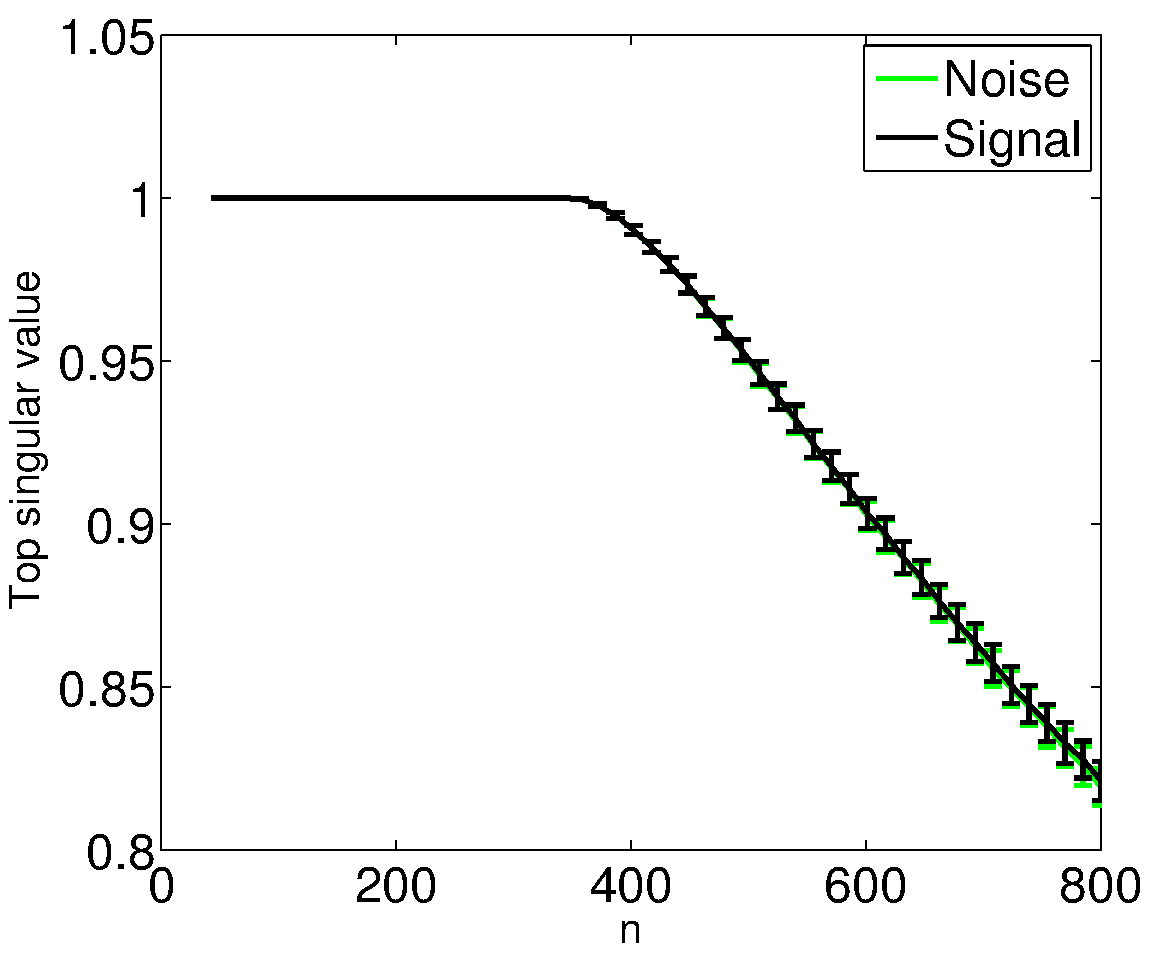
\includegraphics[width=\figwidth]{figures/cca_errorbars_low.pdf}
    \label{fig:cca_errorbars_low_snr}
  }
  \subfigure[$\sigma=3$ dB]{
    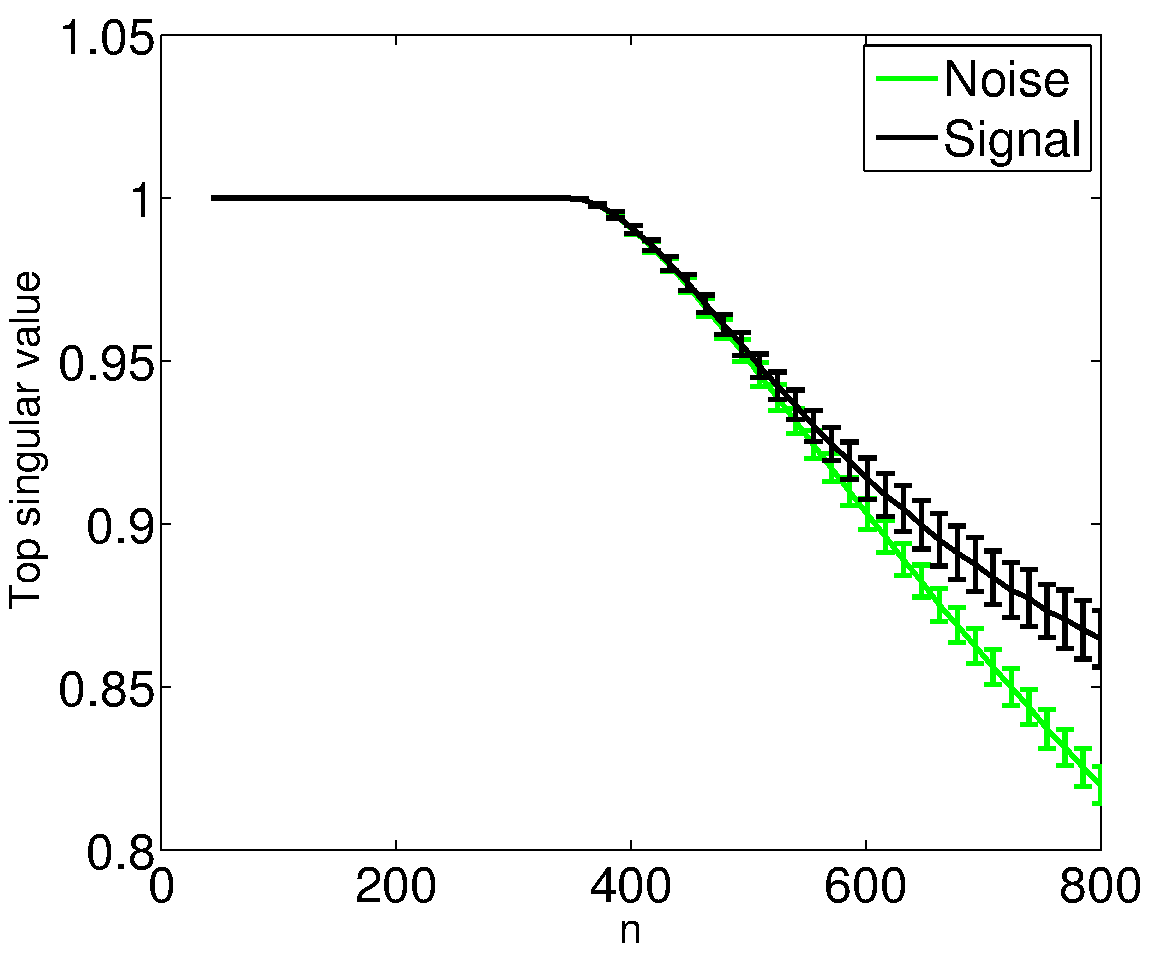
\includegraphics[width=\figwidth]{figures/cca_errorbars_high.pdf}
    \label{fig:cca_errorbars_high_snr}
  }
  \caption{Empirical distribution of the top singular value of $\widehat{C}$ in
    (\ref{eq:cca_chat_svd}) for both noise and signal data models in
    (\ref{eq:cca_data_model1}). Simulations were conducted using $d_1=200$, $d_2=150$, and
    $\rho=0.9$. The top singular value was computed for 500 trials. The mean top singular
    value is plotted with $\pm$ one standard deviation errorbars. }
  \label{fig:cca_errorbars}
\end{figure}

Figure \ref{fig:cca_errorbars} highlights the phenomena presented in
\cite{pezeshki2004empirical}. For $n<350=d_1+d_2$, $\widehat{\rho}$ is identically 1 for
both the noise and signal datasets and for both values of $\sigma$. In Figure
\ref{fig:cca_errorbars_low_snr}, the value of $\sigma$ is small enough so that even when
there are many samples present, the empirical distribution of
$\widehat{\rho}^{\text{noise}}$ follows that of $\widehat{\rho}^{\text{signal}}$. However,
when $\sigma$ is larger, as in Figure \ref{fig:cca_errorbars_high_snr}, the distributions
separate when given enough samples. A natural question to ask is ``Are these distributions
different?'' If the answer is no, then the correlation estimate returned by CCA is
useless, being unable to discern if the correlated datasets contain signal or are simply
noise. Next we reproduce the results of \cite{nadakuditi2011fundamental}, using the
two-sided Kolmorgorov-Smirnov (KS) to determine if the distributions are indeed
different. Figure \ref{fig:cca_ks_heatmap} plots the KS statistic for multiple values of
$\sigma$ and $n$.

\begin{figure}
  \centering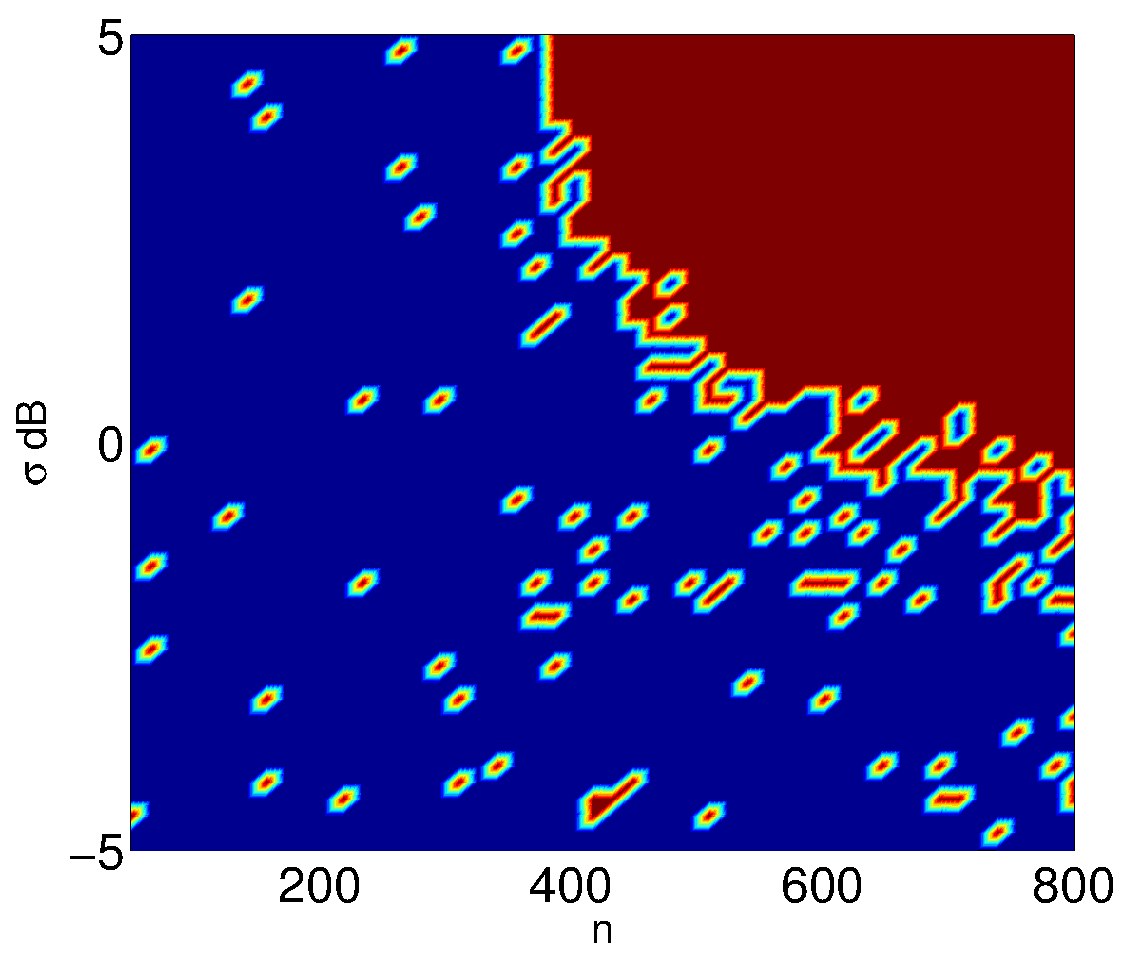
\includegraphics[width=\figwidth]{figures/cca_ks_heatmap.pdf}
  \caption{Two-sided KS statistic between the empirical distributions of the leading
    singular value of $\widehat{C}$ in (\ref{eq:cca_chat_svd}) formed from training data
    generated from the noise and signal data models in (\ref{eq:cca_data_model1}).
    Simulations were conducted using $d_1=200$, $d_2=150$, $\rho=0.9$, 500 trials, and a
    significance level of $\alpha=0.95$ for the KS test. A value of 1 indicates the
    distributions are statistically different while a value of 0 indicates the
    distributions are statistically identical.}
  \label{fig:cca_ks_heatmap}
\end{figure}

This result confirms the result in \cite{nadakuditi2011fundamental}. Two important
consequences follow from Figure \ref{fig:cca_ks_heatmap}. First, it confirms that when
$n<d_1+d_2$ CCA fails to provide meaningful correlation estimates. No matter how large the
value of $\sigma$, CCA will always return a correlation estimate of 1 for any dataset it
is provided. In this sample starved regime, CCA cannot reliably detect the presence of a
signal given two correlated datasets. Second, given $n>d_1+d_2$ samples, there is a
threshold dependent on $n$ such that when $\sigma$ is large enough, the noise and signal
distributions are statistically different and when $\sigma$ is too small, the noise and
signal distributions are statistically identical. The KS statistic determines if the
distributions are statistically distinguishable but gives no insight into \textit{how}
indistinguishable the distributions are. To explore this, we consider constructing a
na\"{\i}ve detector based on the top singular value of $\widehat{C}$. We may construct an
empirical ROC curve of such a detector using the empirical distributions of
$\widehat{\rho}^{\text{noise}}$ and $\widehat{\rho}^{\text{signal}}$. The area under the
ROC curve (AUC) is a measure of the detection ability of such a detector, with 1 being
perfect detection and 0.5 being random guessing. Figure \ref{fig:cca_auc_heatmap} plots
the empirical AUC for such a detector given the empirical distributions for the top
singular value of $\widehat{C}$ under both the noise and signal model.

\begin{figure}
  \centering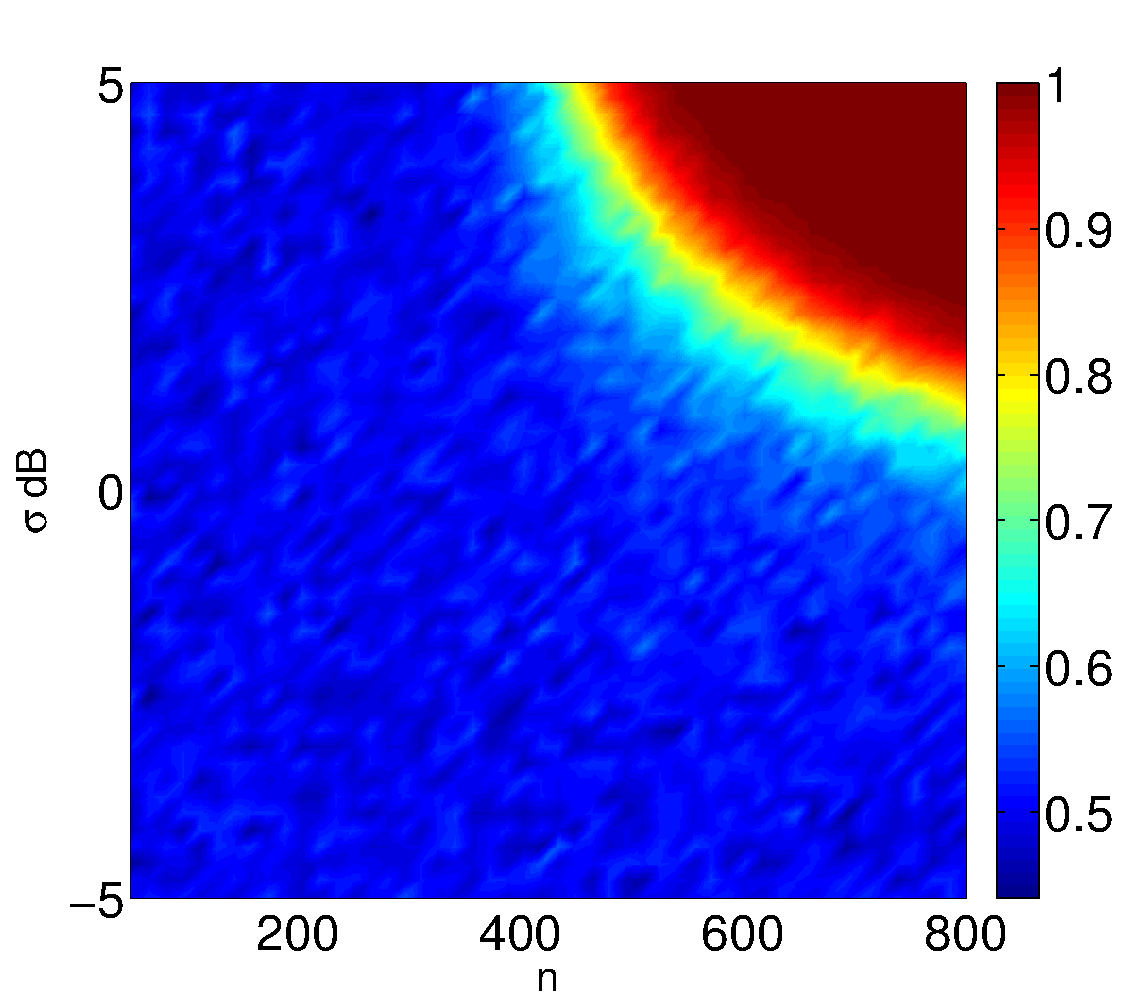
\includegraphics[width=\figwidth]{figures/cca_auc_heatmap.pdf}
  \caption{AUC for a detector based on the top singular value of $\widehat{C}$ in
    (\ref{eq:cca_chat_svd}) to detect the noise and signal data models in
    (\ref{eq:cca_data_model1}). Simulations were conducted using $d_1=200$, $d_2=150$, 500
    trials, and $\rho=0.9$.}
  \label{fig:cca_auc_heatmap}
\end{figure}

This is a new result. While the AUC heatmap in Figure \ref{fig:cca_auc_heatmap} closely
resembles the KS statistic heatmap in Figure \ref{fig:cca_ks_heatmap}, it also provides
information on how far the distributions are separated. When the distributions are
entirely separated, perfect detection is possible, resulting in an AUC of 1. This occurs
for large values of $n$ and $\sigma$. The AUC plot also confirms that when $n<d_1+d_2$,
CCA cannot statistically detect signals given correlated datasets. In fact, a large
portion of the parameter sweep of $n$ and $\sigma$ results in CCA failing.

The breakdown point when $n<d_1+d_2$ is an extremely undesirable property of CCA. In the
low-sample, high dimensional regime, it results in CCA being unable to detect the presence
of a signal given correlated datasets. We demonstrated through numerical simulation that
in this regime the distribution of the leading singular value of noise only datasets is
identical to that of datasets generated with correlated signal. However, using results
from random matrix theory, it is possible to avoid this undesirable performance loss.

\section{Informative CCA (ICCA)}

In \cite{nadakuditi2011fundamental}, Nadakuditi uses recent results from random matrix
theory to derive an informative version of CCA that we will call here informative CCA
(ICCA). Recalling the data SVDs $Y_1=U_1\Sigma_1V_1^H$ and $Y_2=U_2\Sigma_2V_2^H$, random
matrix theory provides the important insight that not all of the right singular vectors
are informative. In particular the following proposition is repeated from
\cite{nadakuditi2011fundamental} for here for reference. Let $z_1=
\left[z_1^{(1)},\dots,z_1^{(n)}\right]^H$ be the correlated signal vector in the first
dataset. 
\begin{prop}\label{prop:raj}
  As $d_1$, $n\to\infty$ with $d_1/n\to c_1$,
  \be
  \left| \left\langle \frac{z_1}{\|z_1\|_2}, V_1(:,1)\right\rangle\right|\convas\begin{cases}
    \varphi_1 & \text{if } \sigma > c_1^{1/4}\\
    0 & \text{otherwise}\\
  \end{cases}, 
  \ee 
  where $\varphi_1:=\sqrt{1 -
    \left(c_1+\sigma^2\right)/\left(\sigma^2\left(\sigma^2+1\right)\right)}$
  \cite{nadakuditi2011fundamental}.
\end{prop}
The analogous theorem holds for the second dataset. The notation $V_1(:,1)$ denotes the
first column of $V_1$. This proposition tells us that there is a critical SNR
$\sigma_{\text{crit}}=\left(\frac{d_1}{n}\right)^{1/4}$ such that if
$\sigma>\sigma_{\text{cirt}}$ the first column of $V_1$ is informative and contains a
portion of the correlated signal $z_1$. However, if $\sigma<\sigma_{\text{crit}}$ the
first column of $V_1$ is uninformative and contains no correlated signal. Such
uninformative components should not be used in CCA as they will degrade its
performance. Following \cite{nadakuditi2011fundamental}, we define the trimmed data
matrices as 
\be\ba
& \widetilde{U}_1 = U(:,1:r_1) && \widetilde{V}_1 = V(:,1:r_1)\\
& \widetilde{U}_2 = U(:,1:r_2) && \widetilde{V}_2 = V(:,1:r_2)\\
\ea\ee 
where $r_1$ and $r_2$ are the number of informative components in the first
and second datasets, respectively.Using these trimmed data matrices, we form the matrix
used for ICCA,
\beq\label{eq:icca_chat}
  \widetilde{C} = \widetilde{U}_1\widetilde{V}_1^H\widetilde{V}_2\widetilde{U}_2^H.
\eeq
Let $\widetilde{C} = \widetilde{F}\widetilde{K}\widetilde{G}^H$ be the SVD of this
matrix. ICCA returns the following informative correlation estimate and canonical vectors
\begin{equation}\label{eq:icca_rho}
\ba
&\widetilde{\rho} &&= \widetilde{k}_1\\
&\widetilde{x}_1 &&= \RIhat^{-1/2}\widetilde{f}_1\\
&\widetilde{x}_2 &&= \RIIhat^{-1/2}\widetilde{g}_1\\
\ea
\end{equation}
We next demonstrate that the correlation estimate returned by ICCA is superior to that
returned by CCA. 

\subsection{Simulation results}

We use the same simulation setup as in the CCA analysis, generating $n$ samples for each
dataset under both the noise and signal model in (\ref{eq:cca_data_model1}). Instead, of
using the estimate $\widehat{C}$, we form the estimates $\widetilde{C}^{\text{noise}}$ and
$\widetilde{C}^{\text{signal}}$ as in (\ref{eq:icca_chat}). First we explore the
distributions of the top singular value, $\widetilde{\rho}^{\text{noise}}$ and
$\widetilde{\rho}^{\text{signal}}$ of these matrices in Figure \ref{fig:icca_errorbars}.

\begin{figure}[h!]
  \centering
  \subfigure[$\sigma=0$ dB]{
    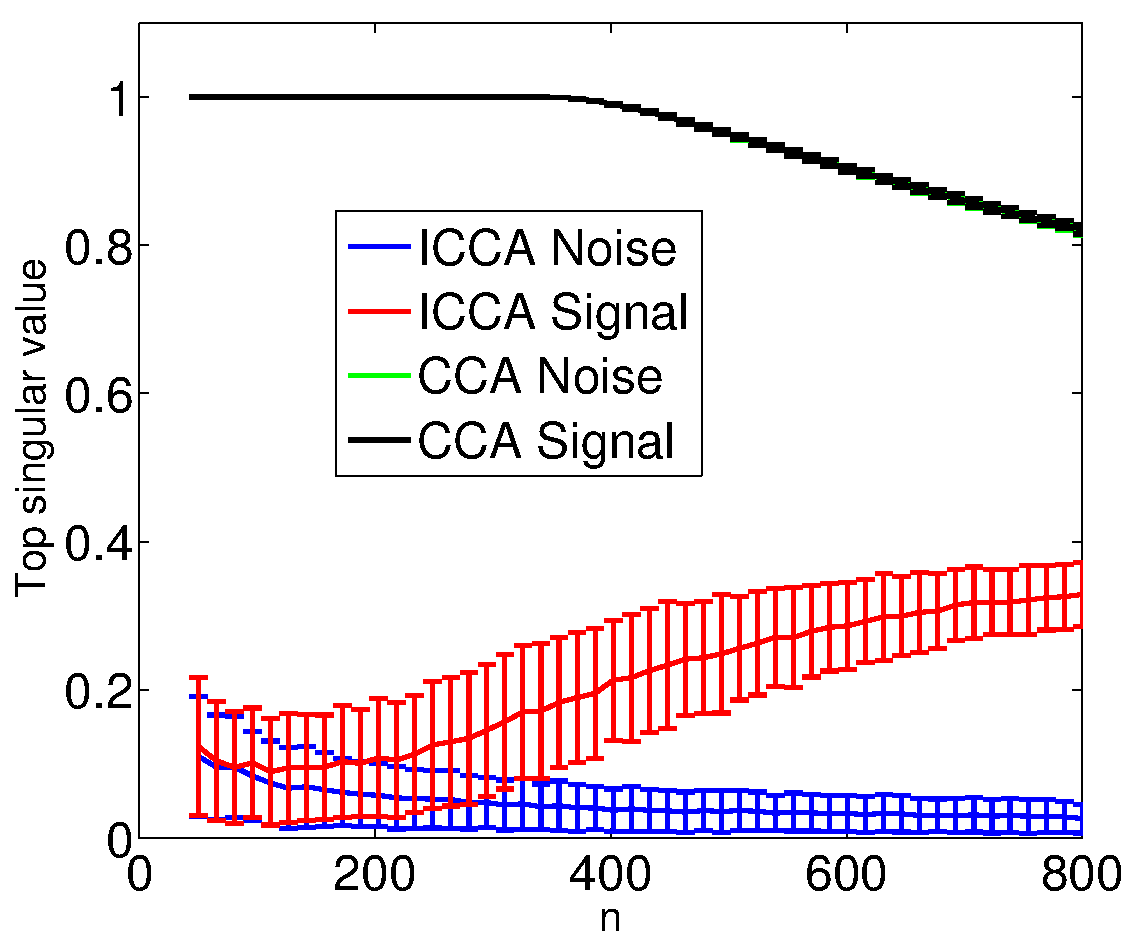
\includegraphics[width=\figwidth]{figures/icca_errorbars_low.pdf}
    \label{fig:icca_errorbars_low_snr}
  }
  \subfigure[$\sigma=3$ dB]{
    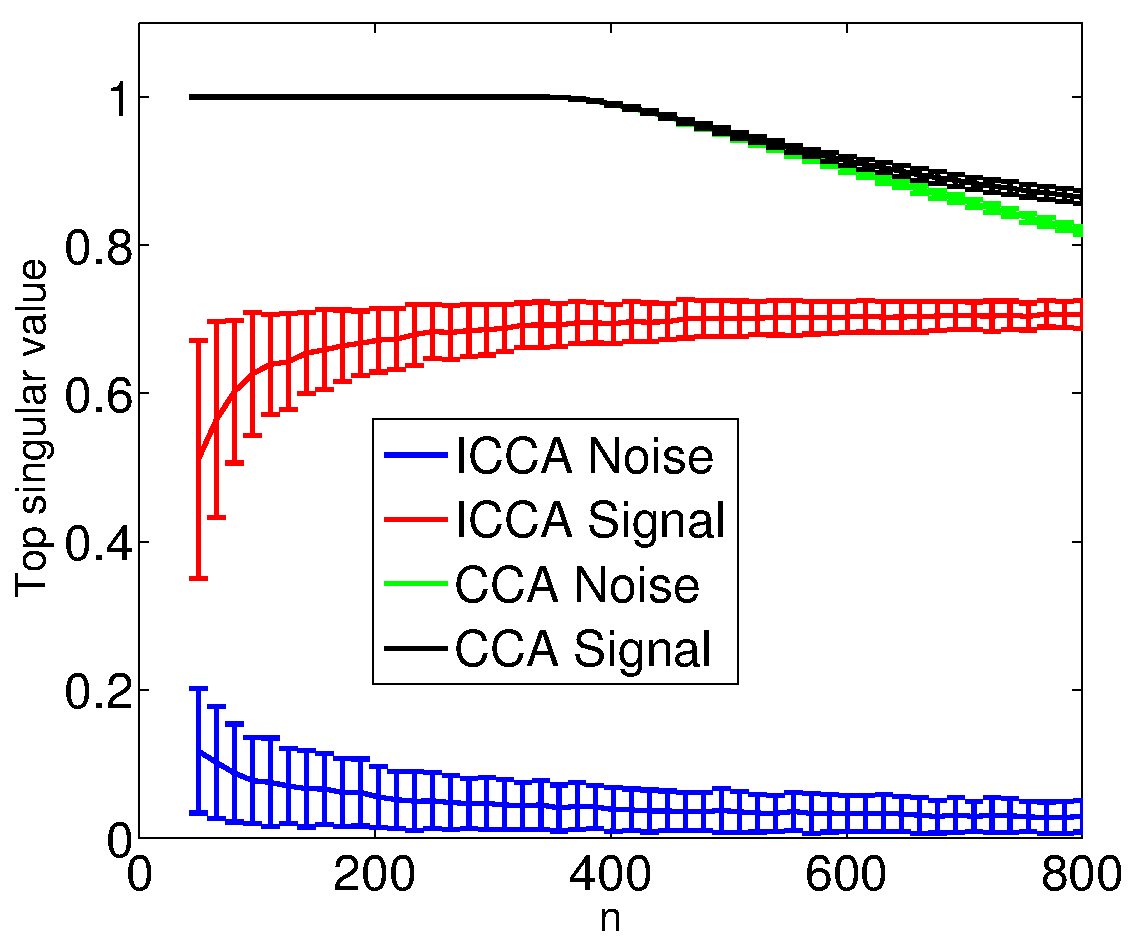
\includegraphics[width=\figwidth]{figures/icca_errorbars_high.pdf}
    \label{fig:icca_errorbars_high_snf}
  }
  \caption{Empirical distribution of the top singular value of $\widetilde{C}$ in
    (\ref{eq:icca_chat}) for both noise and signal data models in
    (\ref{eq:cca_data_model1}). Simulations were conducted using $d_1=200$, $d_2=150$,
    $\rho=0.9$, and $r_1=r_2=1$. The top singular value was computed for 500 trials. The
    mean top singular value is plotted with $\pm$ one standard deviation errorbars.}
  \label{fig:icca_errorbars}
\end{figure}

The results of the empirical distribution of the top singular value of $\widetilde{C}$ are
new. We immediately see many desirable characteristics of ICCA. First, the value of the
top singular value is no longer deterministically 1 when $n<d_1+d_2$. Second, as the
number of available training samples increases, $\tilde{\rho}^{\text{signal}}$ increases
for both values of $\sigma$.  This is desirable because it indicates that with more data,
the estimator is more confident that there is correlation between the dataset. Similarly,
with less data, the estimator is less confident that the datasets are correlated. As the
number of training samples increases, $\widetilde{\rho}^{\text{noise}}$ decreases to 0.
As the noisy datasets are uncorrelated ($\rho=0$), we would like the estimator to indicate
exactly this. The ICCA correlation estimate has this desirable property. Lastly, we note
that ICCA separates the distributions further and with less training data than CCA, even
under low SNR settings. Next, we use the KS statistic to explore when the empirical
distributions of $\widetilde{\rho}^{\text{noise}}$ and $\widetilde{\rho}^{\text{signal}}$
are statistically different. Results are shown in Figure \ref{fig:icca_ks_heatmap} with
the CCA KS heatmap presented again for ease of comparison.

\begin{figure}
  \subfigure[CCA]{
    \centering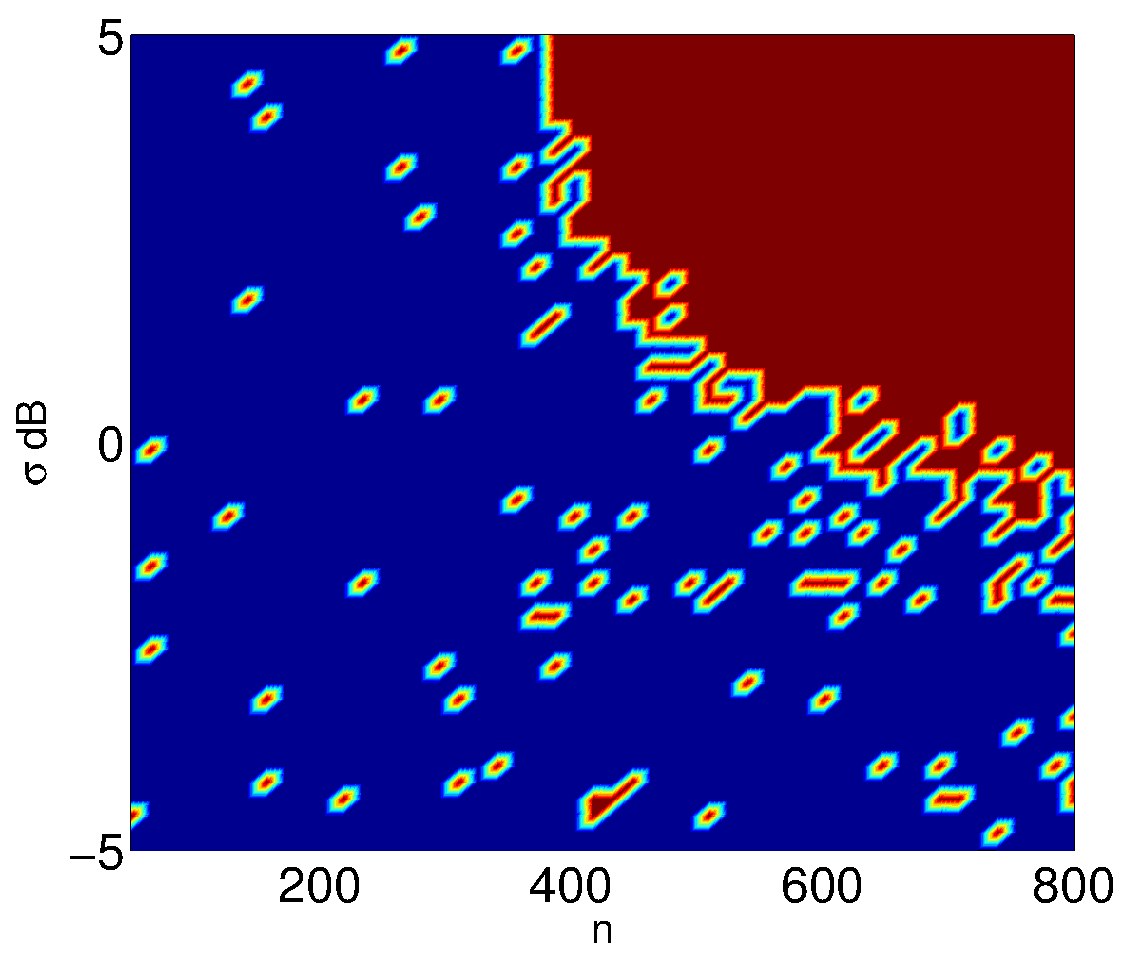
\includegraphics[width=\figwidth]{figures/cca_ks_heatmap.pdf}
  }
  \subfigure[ICCA]{
    \centering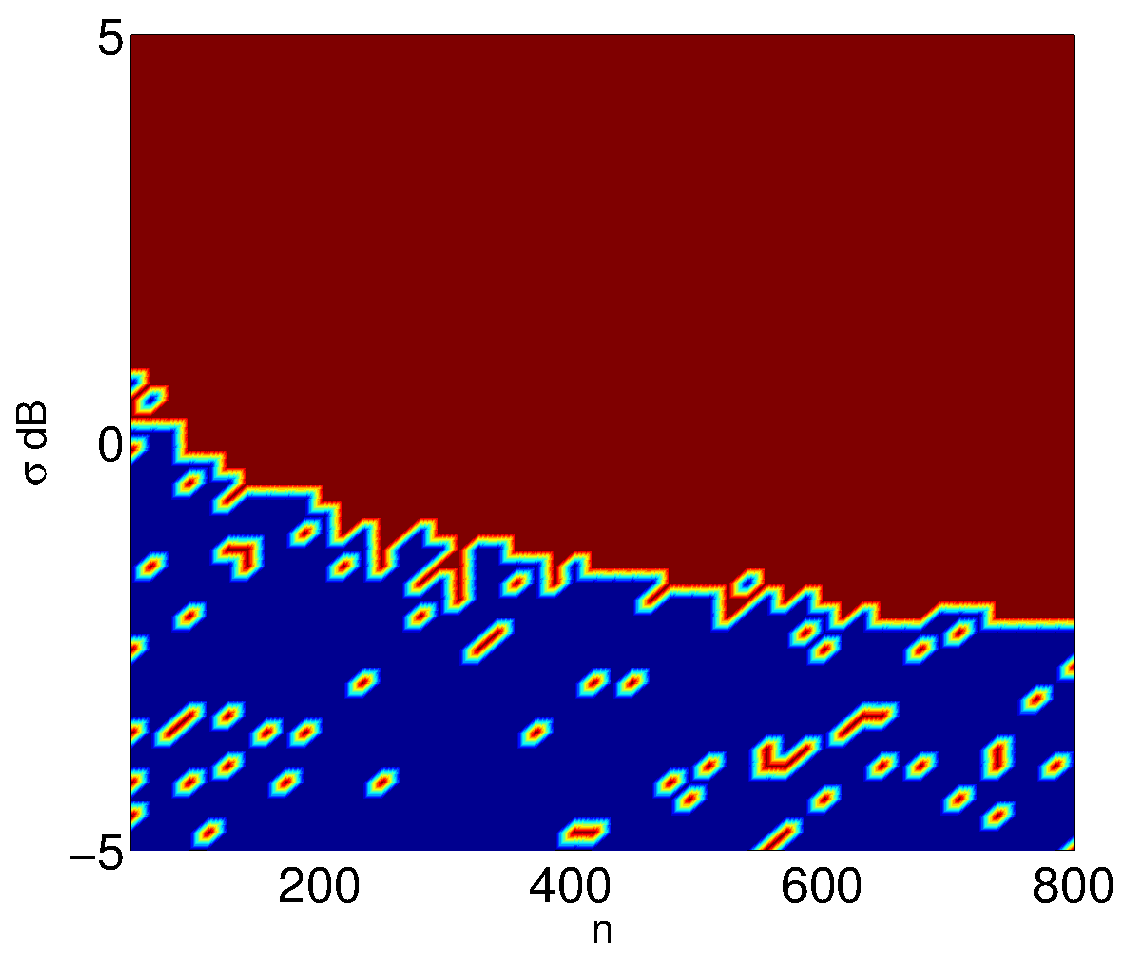
\includegraphics[width=\figwidth]{figures/icca_ks_heatmap.pdf}
  }
  \caption{Two-sided KS statistic between the empirical distributions of the leading
    singular value of $\widetilde{C}$ in (\ref{eq:icca_chat}) formed from training data
    generated from the noise and signal data models in
    (\ref{eq:cca_data_model1}). Simulations were conducted using $d_1=200$, $d_2=150$,
    $\rho=0.9$, $r_1=r_2=1$, 500 trials, and a significance level of $\alpha=0.95$ for the
    KS test. A value of 1 indicates the distributions are statistically different while a
    value of 0 indicates the distributions are statistically identical.}
  \label{fig:icca_ks_heatmap}
\end{figure}

This result confirms the result in \cite{nadakuditi2011fundamental}. Figure
\ref{fig:icca_ks_heatmap} shows that the empirical distributions of
$\widetilde{\rho}^{\text{noise}}$ and $\widetilde{\rho}^{\text{signal}}$ are statistically
different for a much larger number of combinations of $\sigma$ and $n$. In particular,
ICCA does not suffer from the performance breakdown at $n=d_1+d_2$ as CCA does. As one
would desire, given any number of training samples, the ICCA correlation estimates,
$\widetilde{\rho}^{\text{noise}}$ and $\widetilde{\rho}^{\text{signal}}$, are
statistically separable at a sufficiently large enough SNR. Intuitively, this SNR
threshold is larger for smaller values of $n$. For large $n$, ICCA can statistically
separate the distributions of $\widetilde{\rho}^{\text{noise}}$ and
$\widetilde{\rho}^{\text{signal}}$ at a lower SNR as compared to CCA. Finally, we explore
how separable these distributions are by examining the AUC for a na\"{\i}ve detector based
on the empirical correlation estimate returned by ICCA. These results are shown in Figure
\ref{fig:icca_auc_heatmap}. We present the AUC results from CCA again for ease of
comparison.

\begin{figure}
  \subfigure[CCA]{
    \centering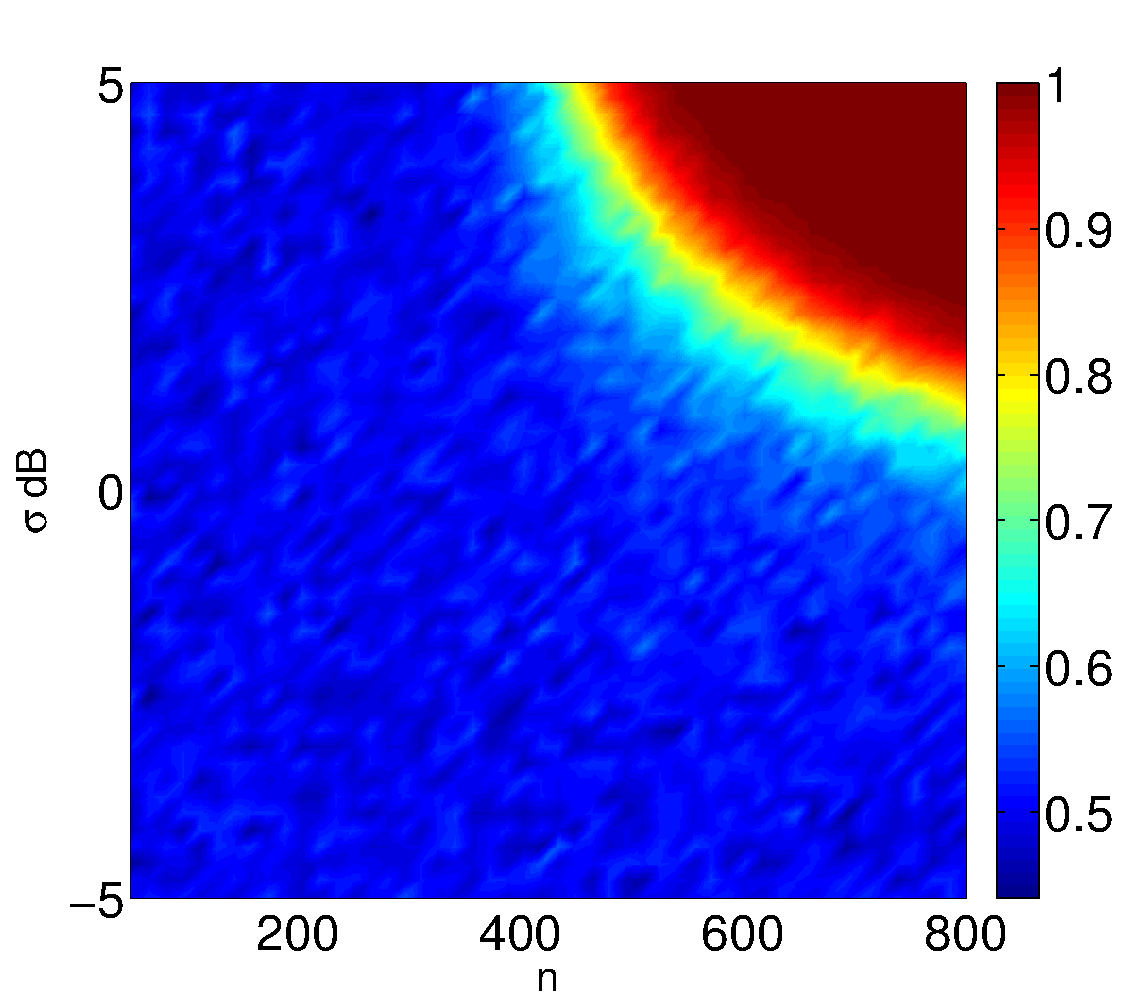
\includegraphics[width=\figwidth]{figures/cca_auc_heatmap.pdf}
  }
  \subfigure[ICCA]{
    \centering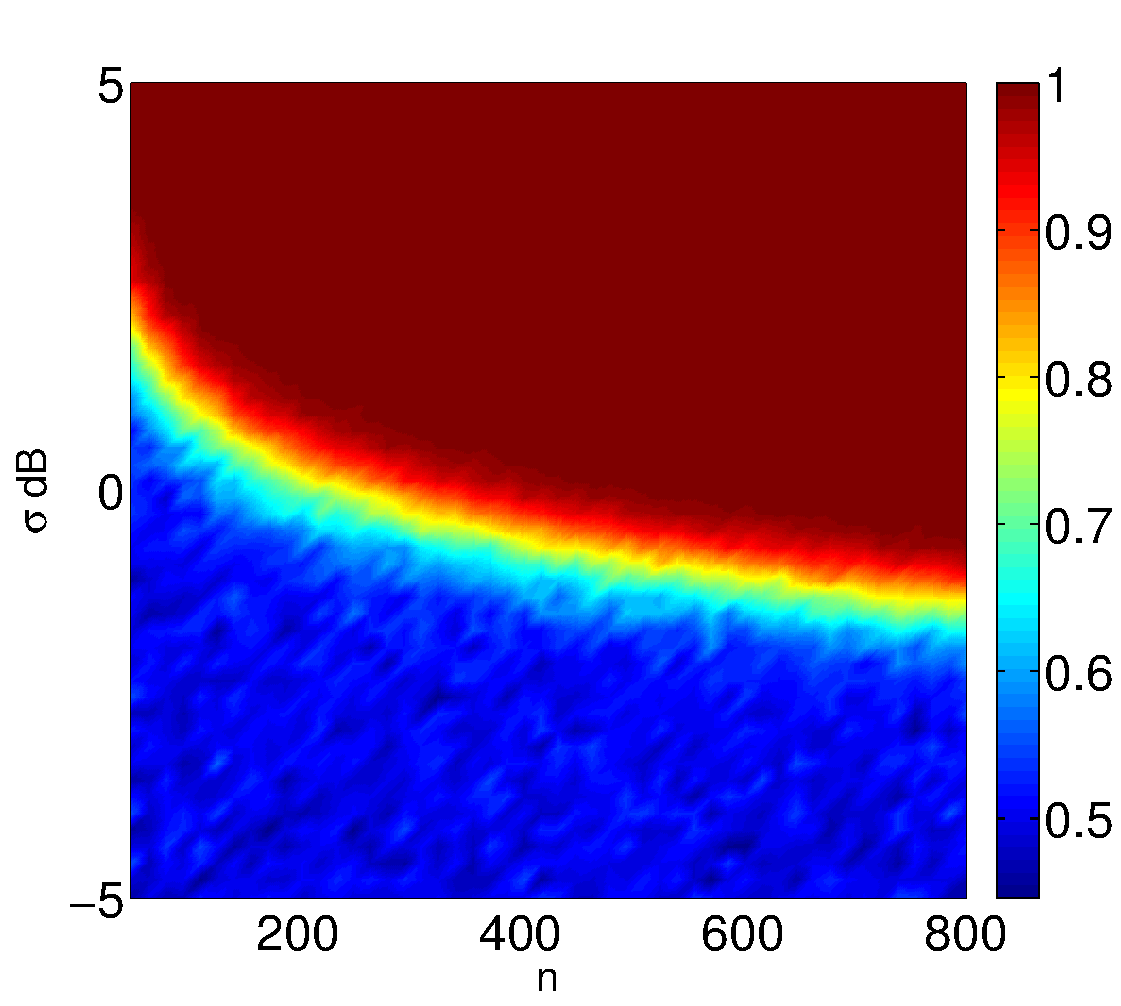
\includegraphics[width=\figwidth]{figures/icca_auc_heatmap.pdf}
  }
  \caption{AUC for a detector based on the top singular value of $\widetilde{C}$ in
    (\ref{eq:icca_chat}) to detect the noise and signal data models in
    (\ref{eq:cca_data_model1}). Simulations were conducted using $d_1=200$, $d_2=150$,
    $\rho=0.9$, 500 trials, and $r_1=r_2=1$.}
  \label{fig:icca_auc_heatmap}
\end{figure}

This is a new result. Similar to the KS statistic results in Figure
\ref{fig:icca_ks_heatmap}, the AUC results in Figure \ref{fig:icca_auc_heatmap} show that
ICCA outperforms CCA for a large number of combinations of $\sigma$ and $n$, most
importantly the sample starved regime. Again, for a fixed $n$, we observe a critical value
of $\sigma$, predicted by Proposition \ref{prop:raj}, above which signal detection is
possible. In the sample rich regime, ICCA can achieve perfect detection (AUC=1) for much
smaller values of SNR, which is highly desirable.

Clearly, the idea of trimming the training data SVDs to only include informative
components used in ICCA is beneficial. ICCA avoids the performance breakdown at
$n<d_1+d_2$ that is present in CCA. Furthermore, ICCA better separates the noise only and
signal distributions of the estimated correlation coefficient. Even in the sample rich
regime when many training data samples are available, ICCA is able to reliably detect
signals at a much lower SNR than CCA. CCA is not used often in the sample starved regime
because of this fundamental performance breakdown. Instead, it is common to use
regularized CCA (RCCA) in such a regime. In Chapter \ref{sec:rcca}, we explore the
performance of RCCA and apply the insights of informative data components to create an
informative version of RCCA. In the next chapter, we investigate applying CCA and ICCA to
matched subspace detection.


\chapter{Low-Rank Gauss-Gauss Detection with Two Datasets}\label{sec:cca_detec}
In this chapter, we develop low-rank Gauss-Gauss detectors when observations from two
datasets are present. In such a setting, each dataset contains a target signal, which is
correlated with the other, that is assumed to reside in a low rank subspace. However, the
observations for each dataset are of high dimension and are corrupted with noise.  When
there is only one dataset present, this problem is referred to as matched subspace
detection. Matched subspace detectors are used in fields such as array processing
\cite{besson2006cfar, besson2005matched}, radar detection \cite{bandiera2007glrt,
  bandiera2007adaptive}, and handwriting recognition \cite{elden2007matrix}. The performance of matched
subspace detectors (MSDs) has been studied extensively when the signal subspace is known
\cite{mcwhorter2003matched, vincent2008matched, scharf1994matched, jin2005cfar} and
recently when the signal subspace is unknown \cite{asendorf2013performance,
  asendorf2012performance}. Here we explore the theory of MSDs when two multi-modal sets
of observations are available. Since these datasets both describe the same system, one
would hope that theoretically fusing feature vectors to account for correlations will
result in better detection ability. This chapter investigates using CCA to determine
whether these observations contain a target signal or whether they are pure noise.

We are motivated by the work in \cite{pezeshki2006canonical}, which shows that the
canonical basis is the right basis to use in low-rank detection. Here, Pezeshki, et
al., consider the signal plus noise model where an observation from one dataset is
available. This observation is a sum of a unknown low rank signal and Gaussian noise. They
apply CCA using the observation as the first modality and the unknown signal as the second
modality. We are interested in the different setting where we are presented with two
datasets, each possibly containing a low rank signal buried in high dimensional noise.

We begin by deriving a standard likelihood-ratio-test (LRT) given both observation
vectors. We then prove that this LRT may be written using the canonical vectors and
correlations returned by CCA. This demonstrates that the CCA basis is a correct basis to
use for Gauss-Gauss detection. We then discuss how to estimate unknown parameters in our
data model and provide empirical, plug-in detectors for both the LRT and CCA
detectors. Using numerical simulations, we demonstrate the extreme sub-optimality of the
empirical CCA detector compared to the plug-in LRT detector. Instead, using an ICCA
detector results in the same performance as the plug-in LRT detector, giving credence to
the previous idea that using only the informative components in data fusion is extremely
important. We provide a proof in the rank-1 setting that the plug-in and ICCA detectors
are equivalent.

\section{Data Model}

Formally, we are given two observation vectors,$y_1$ and $y_2$, of different modalities
(having different features). The goal is to design a detector to distinguish between the
$H_1$ hypothesis that the observations contain a target signal and the $H_0$ hypothesis
that the observations are purely noise. We model our observations by

\beq\label{eq:cca_detect_model} \ba &\text{Noise only, }&&H_0:\left\{ \ba
  & \yI = \xi_1 \\
  & \yII = \xi_2 \\
  \ea\right.\\
&\text{Signal plus noise, }&&H_1:\left\{ \ba
  & \yI = U_1\Sigma_1\,z_1 + \xi_1 \\
  & \yII = U_2\Sigma_2\,z_2 + \xi_2 \\
  \ea\right.\ea \eeq
where $U_1\in\complex^{d_1\times r_1}$ with mutually orthonormal columns,
$U_2\in\complex^{d_2\times r_2}$ with mutually orthonormal columns,
$\Sigma_1=\diag(\sigma_{11},\dots,\sigma_{1r_1})$,
$\Sigma_2=\diag(\sigma_{21},\dots,\sigma_{2r_2})$, with $\sigma_{1i},\sigma_{2i}>0$,
$\xi_1\sim\mathcal{N}(0,I_{d_1})$, $\xi_2\sim\mathcal{N}(0,I_{d_2})$, and 
\be
z=\left[\begin{array}{c}z_1
    \\z_2\end{array}\right]\sim\mathcal{N}\left(0,\left[\begin{array}{cc} I_{r_1} & P \\
      P^H & I_{r_2}\end{array}\right]\right),
\ee
 with $P\in\complex^{r_1\times r_2}$. Let $y=\left[\yI^H\,\yII^H\right]^H$ be the joint
 observation vector, $d=d_1+d_2$ be the dimension of $y$, and $r=r_1+r_2\ll d$ be the combined
 rank of the two low rank signal subspaces. 

\section{LRT Detector Derivation}
We consider the Neyman-Pearson setting for detection (see \cite{van1968detection}) where, given a
test observations from (\ref{eq:cca_detect_model}), we form $y$ as above by stacking the
individual observations in a column vector. The Neyman-Pearson lemma states that a
detector takes the form of a LRT
\beq\label{eq:lrt}
\Lambda(y) := \frac{f\left(y\,|\,H_1\right)}{f\left(y\,|\,H_0\right)}\detgtrless \gamma,
\eeq
where $\Lambda(y)$ is a test statistic, $\gamma$ is a threshold set to achieve a desired
false alarm rate, and $f$ is the appropriate conditional density of the observation.

The conditional distributions of $y$ under each hypothesis are
\be
\ba
& y|H_0 \sim\mathcal{N}(0,I_d) \\
& y|H_1 \sim\mathcal{N}(0,R_y),\\
\ea
\ee
where $R_y=\E{yy^H}$. Substituting these conditional distributions in (\ref{eq:lrt}) , the 
LRT statistic is
\be
\Lambda(y)=\frac{\mathcal{N}(0,R_y)}{\mathcal{N}(0,I_d)},
\ee
which can be simplified to
\beq\label{eq:lrt_stat}
\Lambda(y)=y^H\left(I_d-R_y^{-1}\right)y.
\eeq
The covariance matrix of the observation vector is
\be
\ba
&R_y &&=\left[\begin{array}{cc} \RI & \RIII \\ \RIII^H & \RII\end{array} \right] =
\left[\begin{array}{cc} 
U_1\Sigma_1\Sigma_1^HU_1^H + I_{d_1} &
U_1\Sigma_1P\Sigma_2^HU_2^H \\
U_2\Sigma_2P^H\Sigma_1^HU_1^H &
U_2\Sigma_2\Sigma_2^HU_2^H + I_{d_2} 
\end{array}\right]\\
&&& = \underbrace{\left[\begin{array}{cc}
U_1 & 0 \\ 0 & U_2
\end{array}\right]}_{U}
\underbrace{\left[\begin{array}{cc}
\Sigma_1 & 0 \\ 0 & \Sigma_2
\end{array}\right]}_{\Sigma}
\underbrace{\left[\begin{array}{cc}
    I_{r_1} & P \\ P^H & I_{r_2}
\end{array}\right]}_{R_z}
\underbrace{\left[\begin{array}{cc}
\Sigma_1^H & 0 \\ 0 & \Sigma_2^H
\end{array}\right]}_{\Sigma^H}
\underbrace{\left[\begin{array}{cc}
U_1^H & 0 \\ 0 & U_2^H
\end{array}\right]}_{U^H} + I_d\\
&&& = U\Sigma R_z\Sigma^HU^H + I_d. \\
\ea \ee 
Substituting this covariance matrix into the LRT statistic in (\ref{eq:lrt_stat}),
yields 
\be\ba
&\Lambda(y) &&=y^H\left(I_d-R_y^{-1}\right)y\\
&&& = y^H\left(I_d-\left(U\Sigma R_z\Sigma^HU^H+I_d\right)^{-1}\right)y\\
&&& = y^H\left(I_d-\left(I_d - U\left(\left(\Sigma R_z \Sigma^H\right)^{-1}+
    U^HU\right)\right)^{-1}U^H\right)y\\
&&& = y^H\left(I_d-\left(I_d - U\left(\Sigma^{-1} R_z^{-1} \Sigma^{-H}+I_r
    \right)^{-1}U^H\right)\right)y\\
&&& = y^HU\left(\Sigma^{-1} R_z^{-1} \Sigma^{-H}+I_r
\right)^{-1}U^Hy\\
&&& = y^HU\left(I_k -\Sigma^{-1}\left(R_z+ \Sigma^{-1}\Sigma^{-H}\right)^{-1}\Sigma^{-H}\right)U^Hy.\\
\ea\ee
The LRT detector is
\beq\label{eq:lrt_detect}
\Lambda_\text{lrt}(y) \detgtrless \gamma_{\text{lrt}}
\eeq
where $\Lambda_\text{lrt}(y)=y^HU\left(I_k -\Sigma^{-1}\left(R_z+
    \Sigma^{-1}\Sigma^{-H}\right)^{-1}\Sigma^{-H}\right)U^Hy$ and $\gamma_{\text{lrt}}$ is
a threshold set to satisfy $\Prob{\Lambda_{\text{lrt}}(y) > \gamma_{\text{lrt}}\,|\,H_0} =
\alpha$ where $\alpha$ is a desired false alarm rate. 

Writing the LRT statistic in this form is desirable for computational reasons. Instead of
inverting $R_y$, which is a $d\times d$ matrix of high dimension, we only need to invert
$\Sigma$ and $\left(R_z+ \Sigma^{-1}\Sigma^{-H}\right)$. Since $\Sigma$ is diagonal, its
inverse is easily computed. The second term is a $r\times r$ matrix, where $r\ll d$,
making it much easier to invert than $R_y$. If $y\in\reals^d$ then
\be
\Lambda_{\text{lrt}}(y)= y^HU\left(I_k -\Sigma^{-1}\left(R_z+ \Sigma^{-2}\right)^{-1}\Sigma^{-H}\right)U^Hy.
\ee

%\subsection*{Detectors based on $x$, $y$}
%We will also consider detectors based on the individual observations, $x$ and $y$. In a
%similar derivation, we can show that
%\be\ba
%&\Lambda(x) &&= \frac{\mathcal{N}(0,R_x)}{\mathcal{N}(0,I_p)} = x^H(I_p-R_{xx})x\\
%&&& = x^H\left(U_x\left(\Sigma_x^{-2}+I_{k_x}\right)^{-1}\right)x\\
%&&& = x^HU_x\tilde{\Sigma}_xU_x^Hx\\
%\ea\ee
%where $\tilde{\Sigma}_x=\diag\left(\frac{\sigma_{xi}^2}{\sigma_{xi}^2+1}\right)$.

%Similarly,
%\be
%\Lambda(y) = y^HU_y\tilde{\Sigma}_yU_y^Hy
%\ee
%with $\tilde{\Sigma}_y=\diag\left(\frac{\sigma_{yi}^2}{\sigma_{yi}^2+1}\right)$.

\section{CCA Detector Equivalency}
In this section, we will show that the LRT derived above in (\ref{eq:lrt_detect}) can be
written using the canonical vectors and correlation coefficients found by CCA.

Recall that the matrix of interest in CCA is $C=\RI^{-1/2}\RIII\RII^{-1/2}$ and that the
canonical vectors and correlation coefficients are found by solving the SVD of
$C=FKG^H$. We begin by manipulating the covariance matrix of $y$.

\be\ba
&R_y &&= \left[\begin{array}{cc}
    \RI & \RIII \\ \RIII^H & \RII
\end{array}\right] = 
\left[\begin{array}{cc}
    \RI^{1/2} & 0 \\ 0 & \RII^{1/2}
\end{array}\right]\left[\begin{array}{cc}
  I_{d_1} & C \\ C^H & I_{d_2}
\end{array}\right]\left[\begin{array}{cc}
  \RI^{H/2} & 0 \\ 0 & \RII^{H/2}
\end{array}\right]\\
&&& = \left[\begin{array}{cc}
    \RI^{1/2} & 0 \\ 0 & \RII^{1/2}
\end{array}\right]\left[\begin{array}{cc}
    F & 0\\ 0 & G
\end{array}\right]\left[\begin{array}{cc}
  I_{d_1} & K \\ K^H & I_{d_2}
\end{array}\right]\left[\begin{array}{cc}
    F^H & 0 \\ 0 & G^H
\end{array}\right]\left[\begin{array}{cc}
   \RI^{H/2} & 0 \\ 0 & \RII^{H/2}
\end{array}\right].\\
\ea\ee
Using this decomposition, the inverse of the covariance matrix of $y$ is
\be
R_y^{-1} = \left[\begin{array}{cc}
    \RI^{-1/2} & 0 \\ 0 & \RII^{-1/2}
\end{array}\right]\left[\begin{array}{cc}
    F & 0\\ 0 & G
\end{array}\right]\left[\begin{array}{cc}
    I_{d_1} & K \\ K^H & I_{d_2}
\end{array}\right]^{-1}\left[\begin{array}{cc}
    F^H & 0 \\ 0 & G^H
\end{array}\right]\left[\begin{array}{cc}
    \RI^{-H/2} & 0 \\ 0 & \RII^{-H/2}
\end{array}\right].\\
\ee Recall that the $i$-th canonical vectors returned by CCA are
\be\ba
& \xI^{(i)} = \RI^{-1/2}f_i\\
& \xII^{(i)} = \RII^{-1/2}g_i\\
\ea\ee
 where $f_i$ and $g_i$ are the left and right singular vectors of $C$ corresponding
to the $i$-th largest singular value, $k_i$, respectively. Define the matrices 
\be\ba
&X_1 =\left[\xI^{(1)},\dots, \xI^{(d_1)}\right]= \RI^{-1/2}F
&X_2=\left[\xII^{(1)},\dots,\xII^{(d_2)}\right] = \RII^{-1/2}G
\ea\ee
 to be the matrices of canonical vectors
returned by CCA. Using this notation and substituting the expression for $R_y^{-1}$ in the
LRT statistic in (\ref{eq:lrt_stat}), we arrive at 
\be\ba
&\Lambda(y)&&= y^H\left(I_d -R_y^{-1}\right)y\\
&&&=y^H\left(I_d - \left[\begin{array}{cc} X_1 & 0 \\ 0 & X_2
\end{array}\right]\left[\begin{array}{cc}
    I_{d_1} & K \\ K^H & I_{d_2}
\end{array}\right]^{-1}\left[\begin{array}{cc}
  X_1^H & 0 \\ 0 & X_2^H
\end{array}\right]\right)y.\\
\ea\ee 
The above expression is written in terms of the observation $y$, the canonical
vectors $X_1$ and $X_2$ and the correlation coefficients $K$ returned by CCA. This
statistic is exactly equivalent to the LRT statistic derived earlier. Therefore, we
conclude that the CCA basis is the correct basis to use in such low-rank Gauss-Gauss
detection with two datasets.

We can write this detector slightly differently by recalling that the
canonical variates are $w_1^{(i)}=x_1^{(i)H}y$ and $w_2^{(i)}=x_2^{(i)H}y$. Let
$w_1=\left[w_1^{(1)},\dots,w_1^{(d_1)}\right]^H$,
$w_2=\left[w_2^{(1)},\dots,w_2^{(d_2)}\right]^H$, and define
\be 
w = \left[\begin{array}{c}\wI \\ \wII\end{array}\right] =
\left[\begin{array}{cc}X_1^H & 0 \\ 0 & X_2^H\end{array}\right]y. 
\ee
Using this definition and defining
\be
X = \left[\begin{array}{cc}X_1 & 0 \\ 0 & X_2\end{array}\right],
\ee
the above detector may be written
\beq\label{eq:cca_stat}
\Lambda_{\text{cca}}(w) = w^H\left(\left(X^HX\right)^{-1}-\left[\begin{array}{cc}
    I_{d_1} & K \\ K^H & I_{d_2}
\end{array}\right]^{-1}\right)w.
\eeq
In conclusion, we have derived a general CCA detector that takes the canonical variates as
inputs and uses only the canonical vectors $X$ and the canonical correlation coefficients
$K$ in its statistic. This detector is
\beq\label{eq:cca_detect}
\Lambda_{\text{cca}}\detgtrless\gamma_{\text{cca}}
\eeq
where $\Lambda_{\text{cca}}(w)$ is defined in (\ref{eq:cca_stat}) and
$\gamma_{\text{cca}}$ is a threshold set to satisfy\\
$\Prob{\Lambda_{\text{cca}}(w)>\gamma_{\text{cca}}\,|\,H_0}=\alpha$ where $\alpha$ is the
desired false alarm rate. The CCA detector in (\ref{eq:cca_detect}) is equivalent to the
LRT detector in (\ref{eq:lrt_detect}). This is a general proof and is independent of the
data models placed on $y$. That is, in this proof, we did not refer to the data model in
(\ref{eq:cca_detect_model}) that motivated the problem.

\subsection{CCA Detector for Data Model (\ref{eq:cca_detect_model})}
The above CCA detector was derived for a generic data model. Here we find the canonical
vectors and correlation coefficients for the data model described in
(\ref{eq:cca_detect_model}). Under this model, the data covariance matrices are
\be\ba
&\RI = U_1\Sigma_1\Sigma_1^HU_1^H + I_{d_1}\\
&\RII = U_2\Sigma_2\Sigma_2^HU_2^H + I_{d_2}\\
&\RIII = U_1\Sigma_1P\Sigma_2^HU_2^H\\
\ea\ee
and their inverses are
\be\ba
&\RI^{-1} = \left[\begin{array}{cc}U_1 & U_1^\perp\end{array}\right]
\left[\begin{array}{cc}\left(\Sigma_1\Sigma_1^H + I_{r_1}\right)^{-1} & 0 \\ 0 &
    I_{d_1-r_1} \end{array}\right]  \left[\begin{array}{c} U_1^H \\ U_1^{H\perp} 
  \end{array}\right] \\
&\RI^{-1} = \left[\begin{array}{cc}U_2 & U_2^\perp\end{array}\right]
\left[\begin{array}{cc}\left(\Sigma_2\Sigma_2^H + I_{r_2}\right)^{-1} & 0 \\ 0 &
    I_{d_2-r_2} \end{array}\right]  \left[\begin{array}{c} U_2^H \\ U_2^{H\perp} 
  \end{array}\right]. \\
\ea\ee 
It follows that the CCA matrix $C$ is 
\beq\label{eq:cca_detec_C}\ba
& C &&= \RI^{-1/2}\RIII\RII^{-1/2}\\
&&& = U_1\left(\Sigma_1\Sigma_1^H +I_{r_1}\right)^{-1/2}\Sigma_1 R_z \Sigma_2\left(\Sigma_2\Sigma_2^H+I_{r_2}\right)^{-1/2}U_2^H.\\
\ea\eeq Clearly, when expressed in (\ref{eq:cca_detec_C}), $C$ is a $\min\left(r_1,r_2\right)$ rank
matrix. This implies that there are only $r^*:=\min\left(r_1,r_2\right)$ non-zero correlation
coefficients. Therefore, there are only $r^*$ canonical vectors that should be used in a
detector. Define \be\ba
&X_{1,r^*} = X_1(:,1:r^*)\\
&X_{2,r^*} = X_2(:,1:r^*)\\
&K_{r^*} = K(1:r^*,1:r^*)\\
\ea\ee as the trimmed canonical vectors and correlation coefficients. Finally define 
\be
X_{r^*} = \left[\begin{array}{cc}X_{1,r^*} &0 \\ 0 & X_{2,r^*}\end{array}\right] 
\ee and
$w_{r^*} = X_{r^*}^Hy$. Then the CCA detector is 
\beq\label{eq:cca_stat_r}
\Lambda_{\text{cca}}(w_{r^*}) =
w_{r^*}^H\left(\left(X_{r^*}^HX_{r^*}\right)^{-1}-\left[\begin{array}{cc} I_{r^*} &
      K_{r^*} \\ K_{r^*}^H & I_{r^*} \end{array}\right]^{-1}\right)w_{r^*},
\eeq
which only uses the $r^*$ nonzero CCA correlation coefficients and corresponding 
canonical vectors.

\section{Empirical Detectors}

In many applications, the target signal matrices $U_1$,$U_2$, their SNR matrices
$\Sigma_1$,$\Sigma_2$, and the correlation matrix between datasets $R_z$ are unknown and
thus the resulting data covariance matrices are unknown. Therefore, neither the LRT
statistic in (\ref{eq:lrt_detect}) or the CCA statistic in (\ref{eq:cca_stat_r}), which
relies on $C$ in (\ref{eq:cca_detec_C}) can be computed. In such settings, we are given
training data to estimate any unknown parameters. This section will describe how to
estimate these unknown parameters and use these estimates in the previously derived
detectors. We then will describe how to use ICCA for detection and show its equivalence to
the plug-in LRT detector. Finally, we close with numerical simulations demonstrating that
the ICCA detector achieves the same performance as the plug-in LRT and that the
empirical CCA detector is extremely suboptimal.

\subsection{Parameter Estimation}\label{sec:param_estims}

Assume that we are given $n$ observations of each dataset, $\yI^{(1)},\dots,
\yI^{(n)}$, and $\yII^{(1)},\dots, \yII^{(n)}$. We stack these observations into two
training data matrices $Y_1=\left[\yI^{(1)},\dots, \yI^{(n)}\right]$, and
$Y_2=\left[\yII^{(1)},\dots, \yII^{(n)}\right]$. We assume that $r_1$ and $r_2$ are
known. Let $Q_1D_1V_1^H$ be the SVD of $\frac{1}{\sqrt{n}}Y_1$ and let $Q_2D_2V_2^H$ be
the SVD of $\frac{1}{\sqrt{n}}Y_2$. The ML estimates of our unknown parameters are 

\be\ba
&\widehat{U}_1 = Q_x(:,1:r_1),\,\,\,\widehat{U}_2 = Q_2(:,1:r_2),\,\,\,
\widehat{U}=\left[\begin{array}{cc}\widehat{U}_1 & 0 \\ 0 &
    \widehat{U}_2\end{array}\right]\\
&\widehat{\Sigma}_1 = \left(D_1^2(1:r_1,1:r_1)-I_{r_1}\right)^{1/2},\,\,\, 
\widehat{\Sigma}_2 = \left(D_2^2(1:r_2,1:r_2)-I_{r_2}\right)^{1/2},\,\,\,
\widehat{\Sigma}=\left[\begin{array}{cc}\widehat{\Sigma}_1 & 0 \\ 0 &
    \widehat{\Sigma}_2\end{array}\right]\\
&\RIhat = Q_1D_1D_1^HQ_1^H,\,\,\,
\RIIhat= Q_2D_2D_2^HQ_2^H,\,\,\,
\RIIIhat = Q_1D_1V_1^HV_2D_2^HU_2^H\\
&\widehat{P}=\widehat{\Sigma}_1^{-1}\widehat{U}_1^H\RIIIhat
\widehat{U}_2\widehat{\Sigma}_2^{-1} = \widehat{\Sigma}_1^{-1}D_1(1:r_1,:)
V_1^HV_2D_2(1:r_2,:)^H\widehat{\Sigma}_2^{-1}.\\ 
\ea\ee

\subsection{Rank-1 Detectors}

We consider the most simple setting, when $r_1=r_2=1$ so that $P$ is simply a scalar,
which we will denote $\rho$. In this setting, the parameter estimates simplify to 
\be\ba &
\widehat{U}=\left[\begin{array}{cc}Q_1(:,1) & 0 \\ 0 &
    Q_2(:,1)\end{array}\right]\\
& \widehat{\Sigma}=\left[\begin{array}{cc}\sqrt{d_{11}^2-1} & 0 \\ 0 &
    \sqrt{d_{21}^2 -1}\end{array}\right]\\
& \widehat{P}=\widehat{\rho}=\frac{d_{11}d_{21}V_1(:,1)^HV_2(:,1)}{\sqrt{d_{11}^2
    -1}\sqrt{d_{21}^2-1}} \\
& \widehat{R}_z = \left[\begin{array}{cc}1 &\widehat{\rho}\\ \widehat{\rho} &
    1\end{array}\right]
\ea\ee
where $d_{11}$ is the largest singular value of $Y_1$ and $d_{21}$ is the largest singular
value of $Y_2$. 

To form a realizable LRT detector, we plug in these estimates into the statistic in
(\ref{eq:lrt_stat}). This results in the plug-in LRT statistic
\beq\label{eq:plugin_lrt_stat}
\Lambda_\text{plugin}(y)=y^H\widehat{U}\left(I_2 -\widehat{\Sigma}^{-1}\left(\widehat{R}_z+
    \widehat{\Sigma}^{-1}\widehat{\Sigma}^{-H}\right)^{-1}\widehat{\Sigma}^{-H}\right)
\widehat{U}^Hy.
\eeq

Similarly, we create a realizable CCA detector by performing empirical CCA as described in
Section \ref{sec:emp_cca} by forming 
\be
\widehat{C} =\RIhat^{-1/2}\RIIIhat\RIIhat^{-1/2}=Q_1I_{d_1\times n}V_1^HV_2 I_{n\times
  d_2} Q_2^H.
\ee
We then use the largest (as $r^*=1$) singular value and corresponding left and right
singular vectors of $\widehat{C}$ to form estimates of the canonical vectors and
correlation coefficient. Specifically, let $\widehat{f}_1$ and $\widehat{g}_1$ be the
left and right singular vectors corresponding to the largest singular value
$\widehat{k}_1$. Then the estimates of the canonical vectors and correlation coefficient
are
\beq\label{eq:emp_cca_detec_params}\ba
& \widehat{K}_{r^*} = \widehat{k}_1\\
&\widehat{X}_{r^*} = \left[\begin{array}{cc}\RIhat^{-1/2}\widehat{f}_1 & 0 \\ 0 &
    \RIIhat^{-1/2}\widehat{g}_1\end{array}\right]\\
& \widehat{w}_{r^*} = \widehat{X}_{r^*}^H y.\\
\ea\eeq
We then substitute these estimates into the CCA detector in (\ref{eq:cca_stat_r}).
This results in the empirical CCA detector statistic 
\beq\label{eq:cca_plugin_stat}
\Lambda_{\text{cca}}(\widehat{w}_{r^*}) =
\widehat{w}_{r^*}^H\left(\left(\widehat{X}_{r^*}^H\widehat{X}_{r^*}\right)^{-1} -
  \left[\begin{array}{cc} 1 & \widehat{k}_1 \\ \widehat{k}_1 & 1 \end{array}\right]^{-1}
\right)\widehat{w}_{r^*}.  
\eeq 
However, we saw in Chapter \ref{sec:cca} that empirical
CCA is suboptimal and that we can avoid some of the performance loss of CCA by
informatively trimming data components before computing the canonical vectors. We apply
that principle here to form an ICCA detector. We instead take the top singular value,
$\widetilde{k}_1$ and corresponding singular vectors $\widetilde{f}_1$ and
$\widetilde{g}_1$ of the matrix $\widetilde{C} =
Q_1(:,1)V_1(:,1)^HV_2(:,1)U_2(:,1)^H$. Using this rank-1 SVD, we form informative
canonical vectors and correlation coefficient similarly as in
(\ref{eq:emp_cca_detec_params}). Substituting these informative parameters into the CCA
detector in (\ref{eq:cca_stat_r}) results in the ICCA detector statistic  
\beq\label{eq:icca_plugin_stat} \Lambda_{\text{icca}}(\widetilde{w}_{r^*}) =
\widetilde{w}_{r^*}^H\left(\left(\widetilde{X}_{r^*}^H\widetilde{X}_{r^*}\right)^{-1} -
  \left[\begin{array}{cc} 1 & \widetilde{k}_1 \\ \widetilde{k}_1 & 1 \end{array}\right]^{-1}
\right)\widetilde{w}_{r^*}.  
\eeq

\subsection{Rank 1 Proof that $\Lambda_{\text{icca}}(\widetilde{w}_{r^*})
  \equiv\Lambda_{\text{plug-in}}(y)$}

In this section, we prove that the ICCA detector statistic in (\ref{eq:icca_plugin_stat})
is equivalent to the plug-in LRT statistic in (\ref{eq:plugin_lrt_stat}) when $r^*=r_1=r_2=1$. 
Recall that we are interested in the largest singular value and corresponding singular
vectors of the matrix $\widetilde{C} = Q_1(:,1)V_1(:,1)^HV_2(:,1)U_2(:,1)^H$ used in
ICCA. In the rank-1 setting, $\widetilde{C}$ is a rank-1 matrix, and we immediately
see that $\widetilde{f}_1=Q_1(:,1)$, $\widetilde{g}_1=Q_2(:,1)$, and
$\widetilde{k}_1=V_1(:,1)^HV_2(:,1)$. Therefore, the canonical vectors are
\be\ba
&\widetilde{X}_{r^*} &&= \left[\begin{array}{cc}\RIhat^{-1/2}\widetilde{f}_1 & 0 \\ 0 &
    \RIIhat^{-1/2}\widetilde{g}_1 \end{array}\right]\\
&&& = \left[\begin{array}{cc}\widehat{U}_1\left(\widehat{\Sigma}_1\widehat{\Sigma}_1^H +
      1\right)^{-1/2}  & 0 \\ 0 &
    \widehat{U}_2\left(\widehat{\Sigma}_2\widehat{\Sigma}_2^H  +
      1\right)^{-1/2}\end{array}\right]\\ 
&&& = \widehat{U}\left(\widehat{\Sigma}\widehat{\Sigma}^H + I_{2}\right)^{-1/2}\\
\ea\ee
and the canonical variates are $\widetilde{w}_{r^*} = \widetilde{X}_{r^*}^Hy =
\left(\widehat{\Sigma}\widehat{\Sigma}^H + I_{2}\right)^{-1/2}\widehat{U}^Hy$. Therefore,
we can write the ICCA detector as

\be\ba &\Lambda_{\text{icca}}(\widetilde{w}_{r^*}) &&=
\widetilde{w}_{r^*}^H\left(\left(\widetilde{X}_{r^*}^H\widetilde{X}_{r^*}\right)^{-1} -
  \left[\begin{array}{cc} 1 & \widetilde{k}_1 \\ \widetilde{k}_1 &
      1 \end{array}\right]^{-1}
\right)\widetilde{w}_{r^*}\\
&&& = y^H\widehat{U}\left(\widehat{\Sigma}\widehat{\Sigma}^H + I_{2}\right)^{-1/2}\left(
  \left(\widehat{\Sigma}\widehat{\Sigma}^H + I_2\right) - \left[\begin{array}{cc} 1 &
      \widetilde{k}_1 \\ \widetilde{k}_1 & 1 \end{array}\right]^{-1}
\right)\left(\widehat{\Sigma}\widehat{\Sigma}^H + I_{2}\right)^{-1/2}\widehat{U}^Hy\\
&&& = y^H\widehat{U}\left(I_2 - \left(\widehat{\Sigma}\widehat{\Sigma}^H +
    I_{2}\right)^{-1/2} \left[\begin{array}{cc} 1 & \widetilde{k}_1 \\ \widetilde{k}_1 &
      1 \end{array}\right]^{-1}\left(\widehat{\Sigma}\widehat{\Sigma}^H +
    I_{2}\right)^{-1/2}\right)\widehat{U}^Hy\\
&&& = y^H\widehat{U}\left(I_2 - \left[\begin{array}{cc}
      \widehat{\Sigma}_1\widehat{\Sigma}_1^H + 1 &
      d_{11}\widetilde{k}_1d_{21} \\
      d_{21}\widetilde{k}_1d_{11} & \widehat{\Sigma}_2\widehat{\Sigma}_2^H
      +1 \end{array}\right]^{-1}\right)\widehat{U}^Hy\\
&&& = y^H\widehat{U}\left(I_2 - \left[\begin{array}{cc}
      \widehat{\Sigma}_1\widehat{\Sigma}_1^H + 1 & d_{11}V_1(:,1)^HV_2(:,1)d_{21} \\
      d_{21}V_2(:,1)^HV_1(:,1)d_{11} & \widehat{\Sigma}_2\widehat{\Sigma}_2^H
      +1 \end{array}\right]^{-1}\right)\widehat{U}^Hy\\
&&& = y^H\widehat{U}\left(I_2 - \left(\widehat{\Sigma}\left[\begin{array}{cc} 1 &
        \widehat{P} \\ \widehat{P}^H &
        1  \end{array}\right]\widehat{\Sigma}^H+I_2\right)^{-1}\right)\widehat{U}^Hy\\
&&& = y^H\widehat{U}\left(I_2 - \left(\widehat{\Sigma}\widehat{R}_z
    \widehat{\Sigma}^H+I_2\right)^{-1}\right)\widehat{U}^Hy\\
&&& = y^H\widehat{U}\left(I_2 - \widehat{\Sigma}^{-1}\left(\widehat{R}_z +
    \widehat{\Sigma}^{-1}\widehat{\Sigma}^{-H}\right)^{-1}\widehat{\Sigma}^{-1}
\right)\widehat{U}^Hy.\\
\ea\ee

This is exactly the expression for the plug-in LRT statistic.

\subsection{Rank 1 Numerical Simulations}

We now use numerical simulations to explore the performance of the plug-in LRT detector in
(\ref{eq:plugin_lrt_stat}), the empirical CCA detector in (\ref{eq:icca_plugin_stat}), and
the ICCA detector in (\ref{eq:cca_plugin_stat}) in the rank-1 setting where
$r_1=r_2=1$. Specifically, we wish to show that the plug-in LRT detector is
equivalent to the ICCA detector. We also wish to explore how the performance of the
CCA detector in compares to that of the plug-in LRT detector, because in theory these
detectors are equivalent.

To compare the performance of these detectors, we compute empirical ROC curves. To
compute an empirical ROC curve, we first generate  two random signal vectors, $u_1$ and
$u_2$, by taking the first left singular vector of two appropriately sized random
matrices with i.i.d. $\mathcal{N}(0,1)$ entries. In this simulation we make the
simplifying assumption that $\sigma_1=\sigma_2$. Given a desired SNR, correlation $\rho$,
and random $u_1$ and $u_2$, we generate $n$ training samples of $\yI$ and $\yII$ from the
$H_1$ hypothesis in (\ref{eq:cca_detect_model}). Using these training samples, we form
estimates $\widehat{U}$, $\widehat{\Sigma}$, $\widehat{\rho}$, $\RIhat$, $\RIIhat$, and
$\RIIIhat$ as described in Section \ref{sec:param_estims}.

We then generate a desired number of test samples from each hypothesis using
(\ref{eq:cca_detect_model}). For each test sample, we compute the test statistic for the
plug-in LRT, empirical CCA, and ICCA detectors in (\ref{eq:plugin_lrt_stat}),
(\ref{eq:cca_plugin_stat}), and (\ref{eq:icca_plugin_stat}), respectively. Using Fawcett's
\cite{fawcett2006introduction} `Algorithm 2', we compute an empirical ROC curve by first
sorting the test statistics for a given detector. At each statistic, we log a ($P_F$,
$P_D$) pair by counting the number of lower scores generated from each hypothesis. This is
repeated for multiple realizations of $u_1$ and $u_2$, generating multiple empirical ROC
curves for each detector. We refer to a single empirical ROC curve corresponding to a
realization of $u_1$ and $u_2$ as a trial. We then average the empirical ROC curves for a
detector over multiple trials using Fawcett's \cite{fawcett2006introduction} `Algorithm
4'. This performs threshold averaging by first uniformly sampling the sorted list of all
test scores of ROC curves and then computing ($P_F$, $P_D$) pairs in the same way as
`Algorithm 2'.

To compare the ROC curves of different detectors, we use the area under the ROC curve
(AUC) statistic. The AUC statistic ranges between 0.5, which represents a random guessing
detector, and 1.0, which represents a detector that can perfectly distinguish between the
two hypotheses. We compute the ROC curves and their respective AUC for many values of the
number of training samples, $n$, and SNR $\sigma=\sigma_1=\sigma_2$. We present the AUC
results in the form of a heatmap for two different values of $\rho$ for each of the
detectors. Figure \ref{fig:auc_high_rho} presents results for $\rho=0.8$ and Figure
\ref{fig:auc_low_rho} presents results for $\rho = 0.2$.

\begin{figure} 
  \subfigure[Plug-in LRT]{
    \centering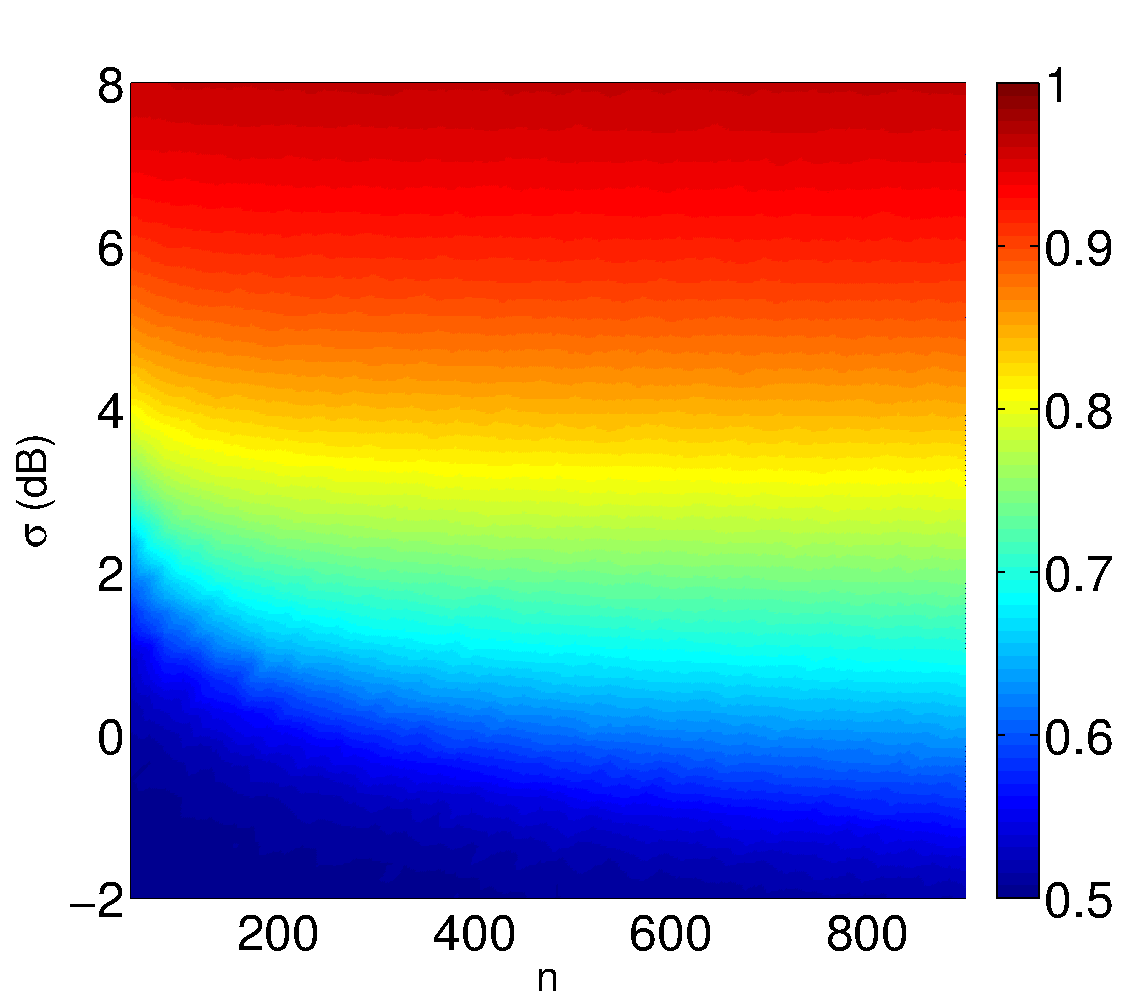
\includegraphics[width=\figwidth]{figures/auc_lrt_high_rho.pdf}
    \label{fig:auc_lrt_high_rho}
  }
  \subfigure[ICCA]{
    \centering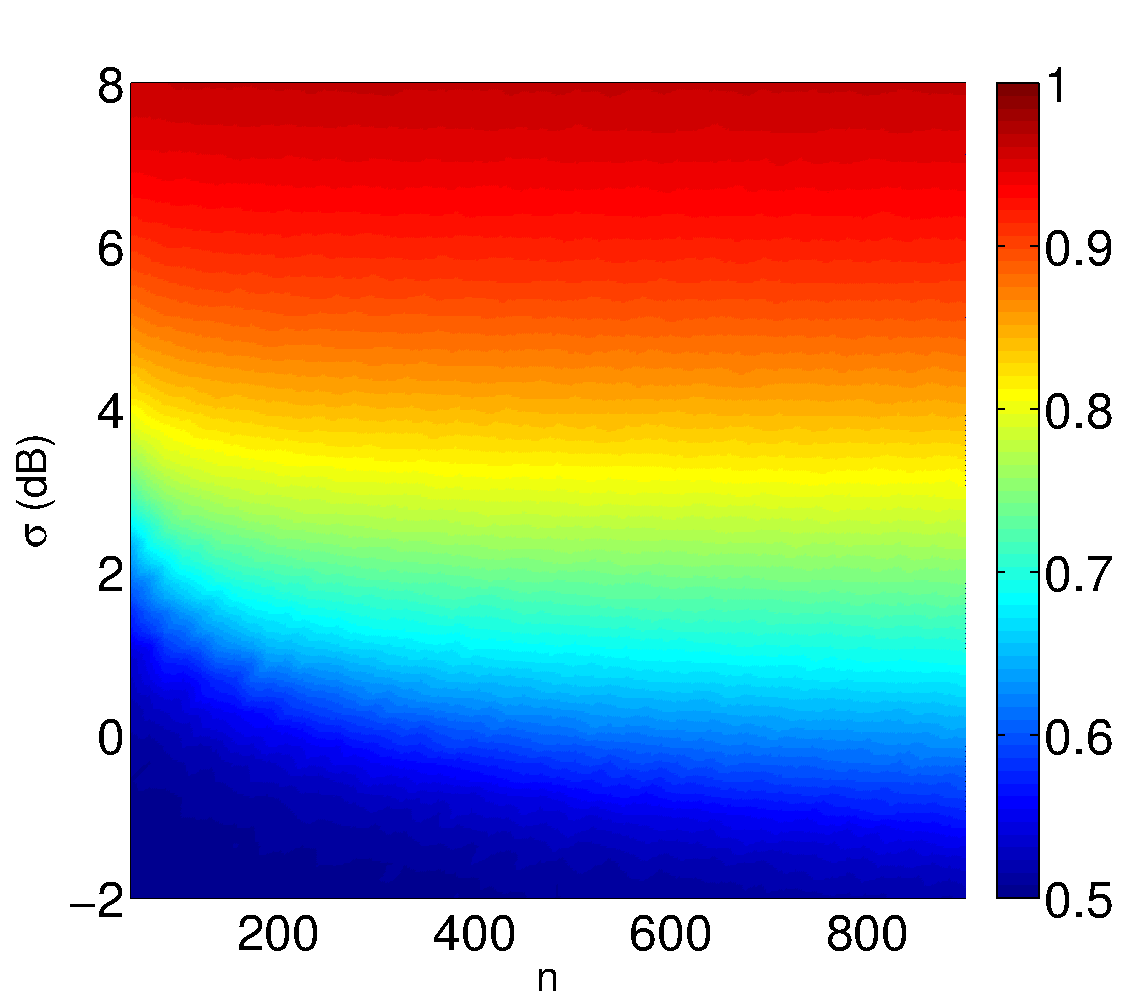
\includegraphics[width=\figwidth]{figures/auc_icca_high_rho.pdf}
    \label{fig:auc_icca_high_rho}
  }
  \subfigure[Empirical CCA]{
    \centering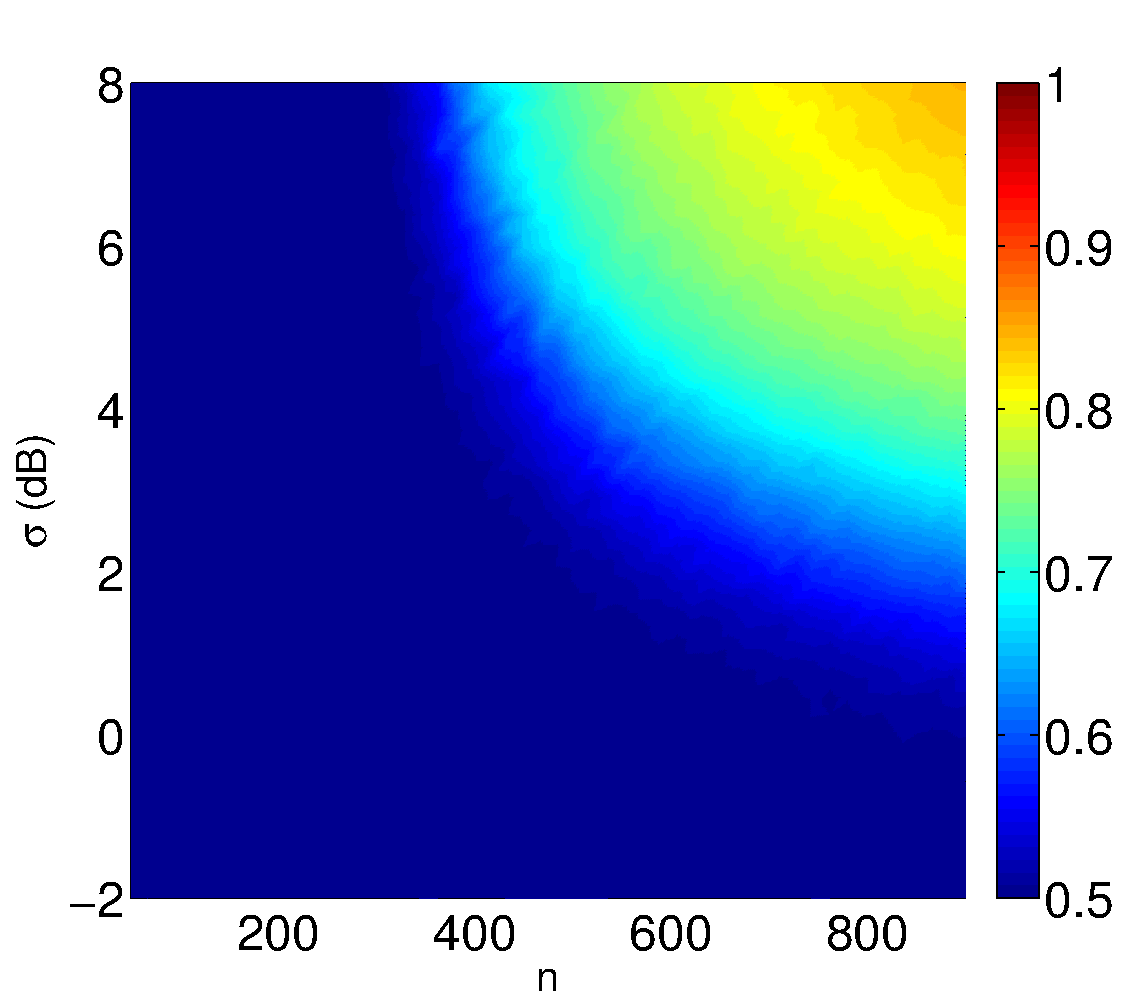
\includegraphics[width=\figwidth]{figures/auc_cca_high_rho.pdf}
    \label{fig:auc_cca_high_rho}
  }
  \caption{AUC results for the plug-in LRT, empirical CCA, and ICCA detectors in
    (\ref{eq:plugin_lrt_stat}), (\ref{eq:cca_plugin_stat}), and
    (\ref{eq:icca_plugin_stat}), respectively. Empirical ROC curves were simulated using
    $2000$ test samples for each hypothesis and averaged over $50$ trials using
    algorithms 2 and 4 of \cite{fawcett2006introduction}. Simulations parameters were
    $d_1=200$, $d_2=150$, and $\rho=0.8$. Each figure plots the AUC for the average ROC curve
    at a different values of SNR, $\sigma=\sigma_1=\sigma_2$, and training samples, $n$.}
  \label{fig:auc_high_rho}
\end{figure}

\begin{figure} 
  \subfigure[Plug-in LRT]{
    \centering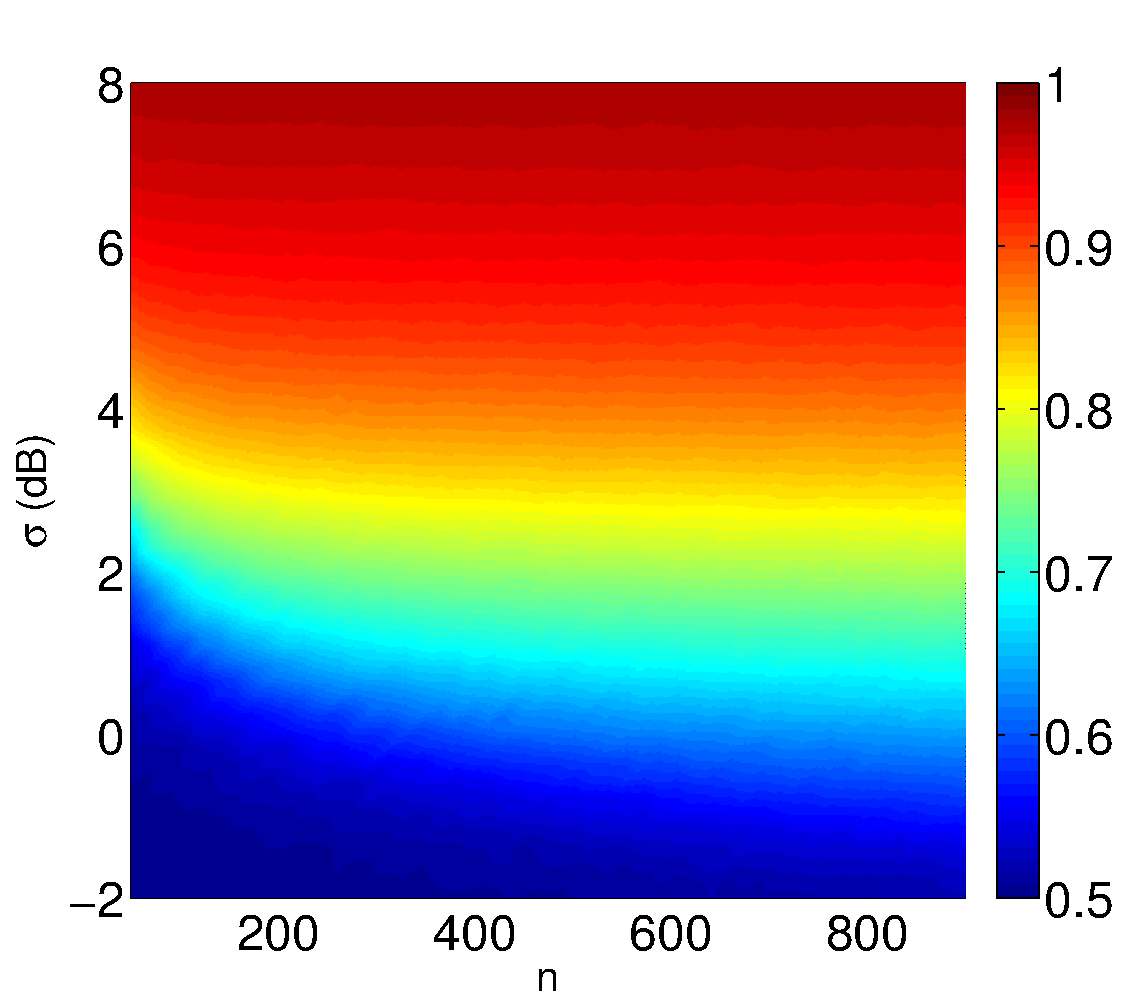
\includegraphics[width=\figwidth]{figures/auc_lrt_low_rho.pdf}
    \label{fig:auc_lrt_low_rho}
  }
  \subfigure[ICCA]{
    \centering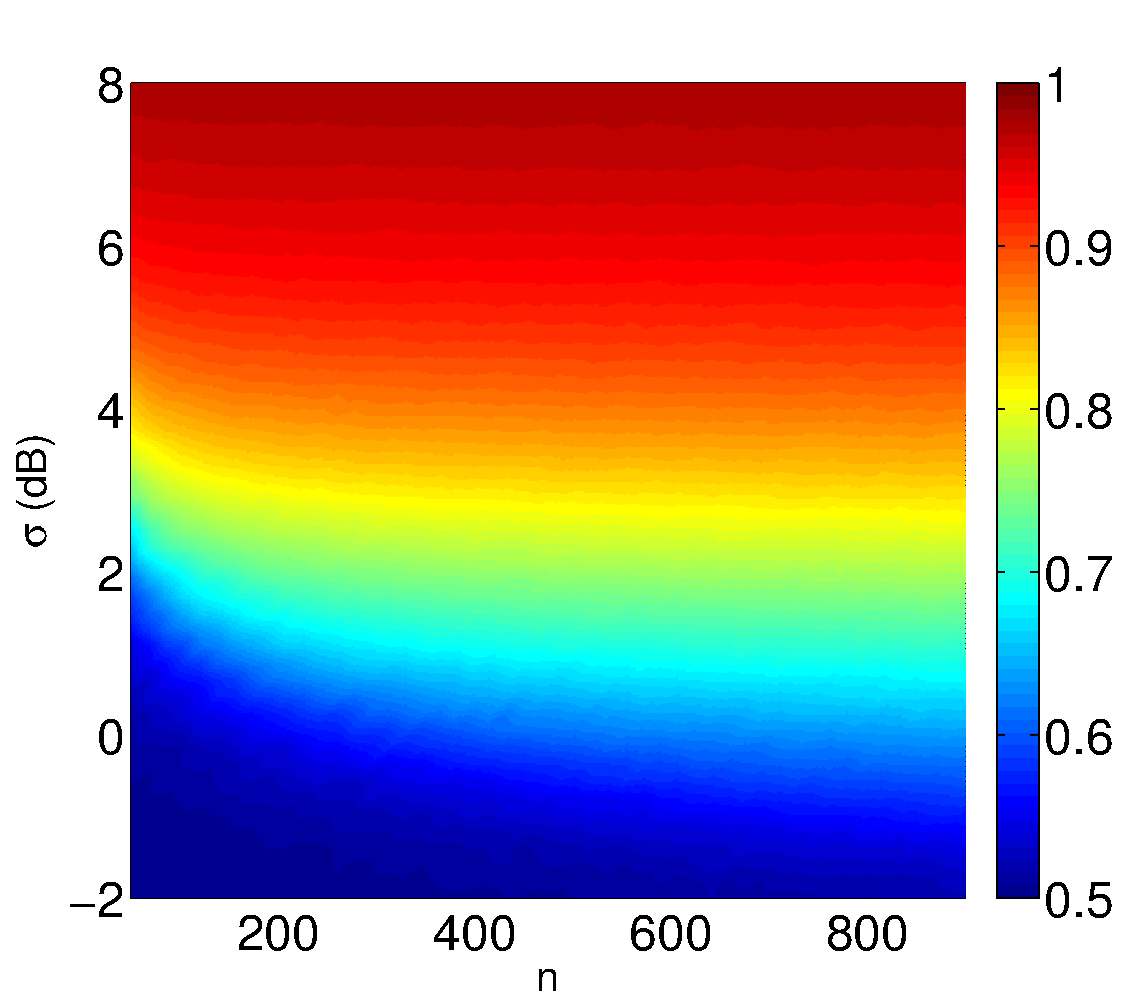
\includegraphics[width=\figwidth]{figures/auc_icca_low_rho.pdf}
    \label{fig:auc_icca_low_rho}
  }
  \subfigure[CCA]{
    \centering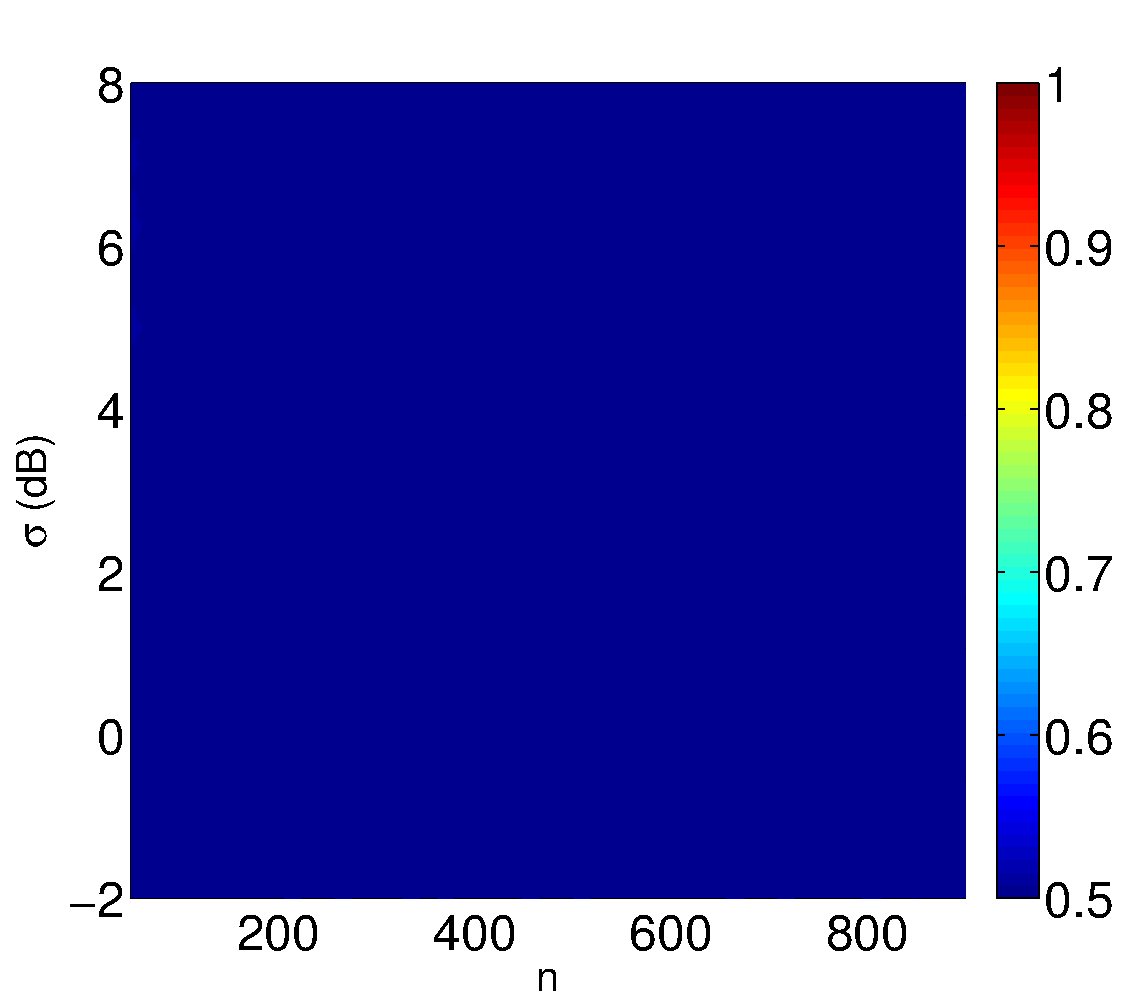
\includegraphics[width=\figwidth]{figures/auc_cca_low_rho.pdf}
    \label{fig:auc_cca_low_rho}
  }
  \caption{AUC results for the plug-in LRT, empirical CCA, and ICCA detectors in
    (\ref{eq:plugin_lrt_stat}), (\ref{eq:cca_plugin_stat}), and
    (\ref{eq:icca_plugin_stat}), respectively. Empirical ROC curves were simulated using
    $2000$ test samples for each hypothesis and averaged over $50$ trials using
    algorithms 2 and 4 of \cite{fawcett2006introduction}. Simulations parameters were
    $d_1=200$, $d_2=150$, and $\rho=0.2$. Each figure plots the AUC for the average ROC curve
    at a different value of SNR, $\sigma=\sigma_1=\sigma_2$, and training samples, $n$.}
  \label{fig:auc_low_rho}
\end{figure}

Evident in both Figures \ref{fig:auc_high_rho} and \ref{fig:auc_low_rho}, the ICCA
detector exhibits the same AUC performance as the plug-in LRT for both values of
$\rho$. This confirms the derivation in the above section. In Figure
\ref{fig:auc_high_rho}, we observe that the CCA detector is extremely suboptimal in the
sample and SNR regime presented. When $n<350=d_1+d_2$, the CCA detector degrades to random
guessing, evident in an AUC of 0.5. The results presented in Chapter
\ref{sec:cca} show that in this sample poor regime, the correlation coefficient
estimate returned by CCA is deterministically 1. It is of no surprise that the subsequent
CCA detector is useless in this regime. Even when $n>d_1+d_2$, the CCA detector achieves a
lower AUC than the ICCA detector. The ICCA detector can tolerate a much lower SNR to achieve
the same AUC performance as the CCA detector.

When decreasing $\rho$ in Figure \ref{fig:auc_low_rho}, the CCA detector observes an even
further performance loss. In the training sample and SNR parameter regime presented,
the CCA detector achieves an AUC of 0.5, indicating it is useless in detection. However,
the plug-in LRT and ICCA detectors show a slight increase in AUC performance. The
intuitive explanation for this result is that decreasing the value of $\rho$ makes the
observations $\yI$ and $\yII$ more independent. Therefore, these observations contain more
information and thus increase detection performance. 

These results are particularly surprising because we began this chapter by deriving the
fact that the LRT detector is equivalent to the CCA detector. However, when using
parameter estimates, the empirical CCA detector no longer is equivalent to the plug-in
detector. As many applications require estimating the covariance matrices used in CCA,
this is an extremely undesirable property of CCA. However, using only the informative
components from our training data, as ICCA does, results in equivalent performance as the
plug-in CCA detector. This performance loss of the empirical CCA detector can be avoided.


%\section*{Performance Loss Heatmaps}

%Defining performance loss for a fixed $P_F$ to be
%\begin{equation}
%  \epsilon = 1 - \frac{P_D^{\text{achieved}}}{P_D^{oracle}}
%\end{equation}

%The following results are for $P_F=0.1$

%\begin{figure} 
%\centering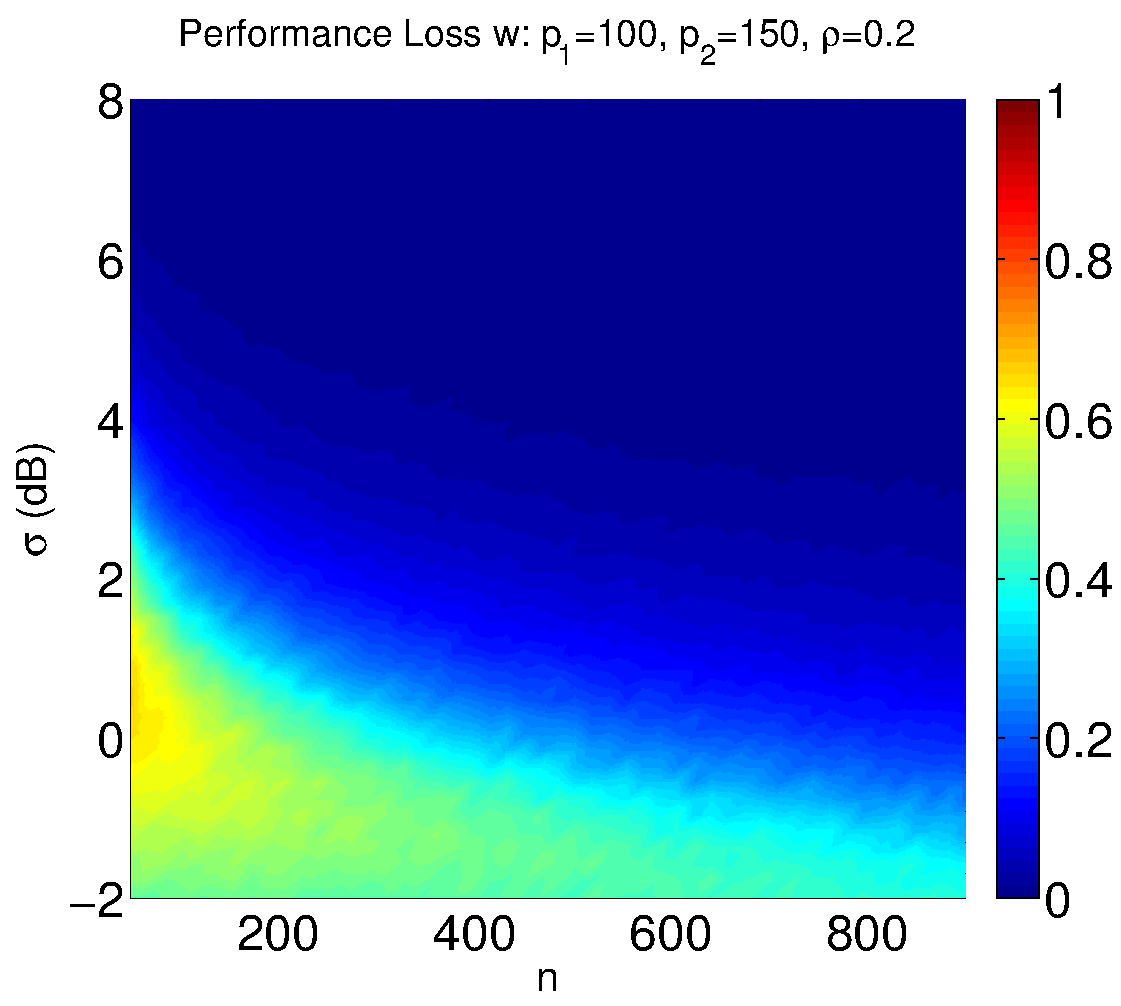
\includegraphics[width=4in]{figures/pl_w_small.pdf}
%\end{figure}

%\begin{figure} 
%\centering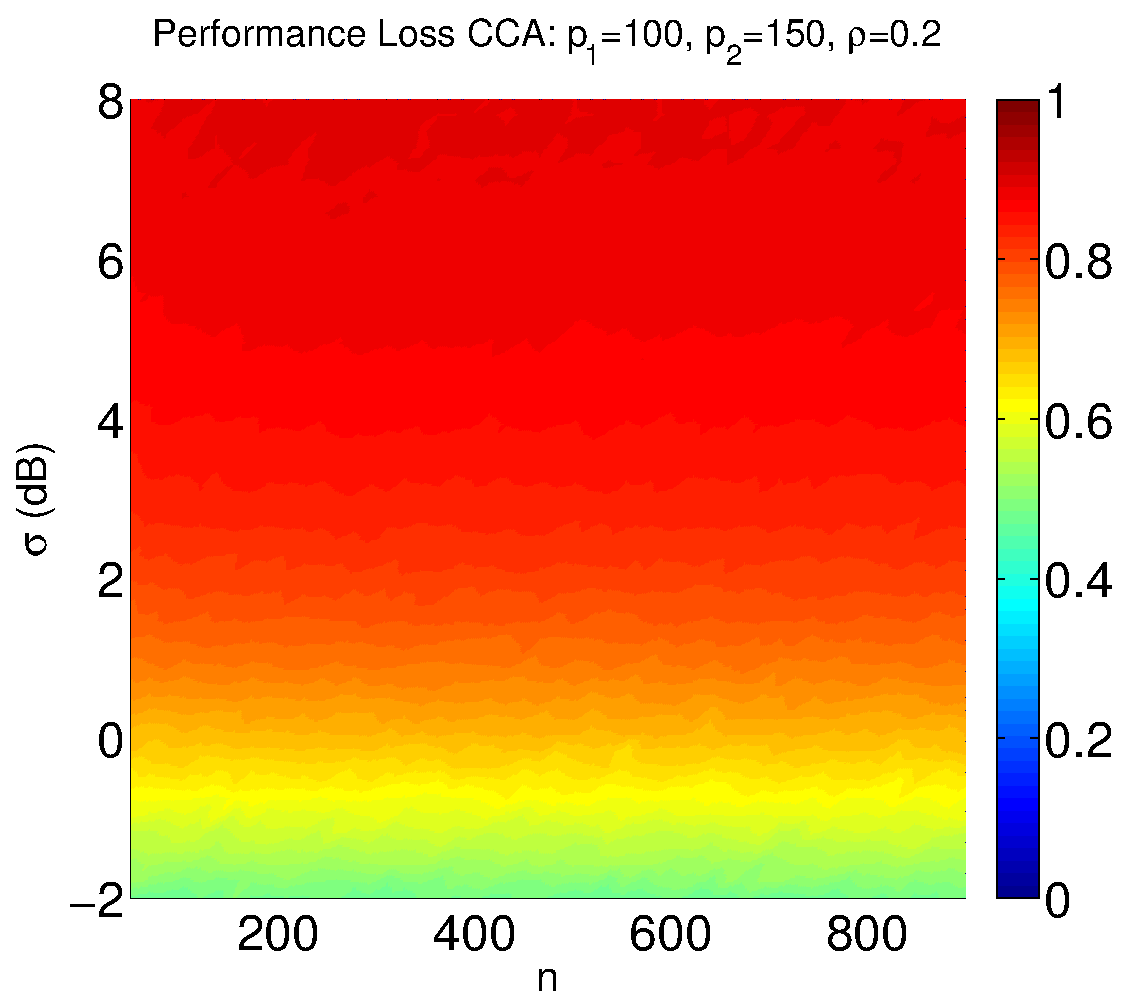
\includegraphics[width=4in]{figures/pl_cca_small.pdf}
%\end{figure}

%\begin{figure} 
%\centering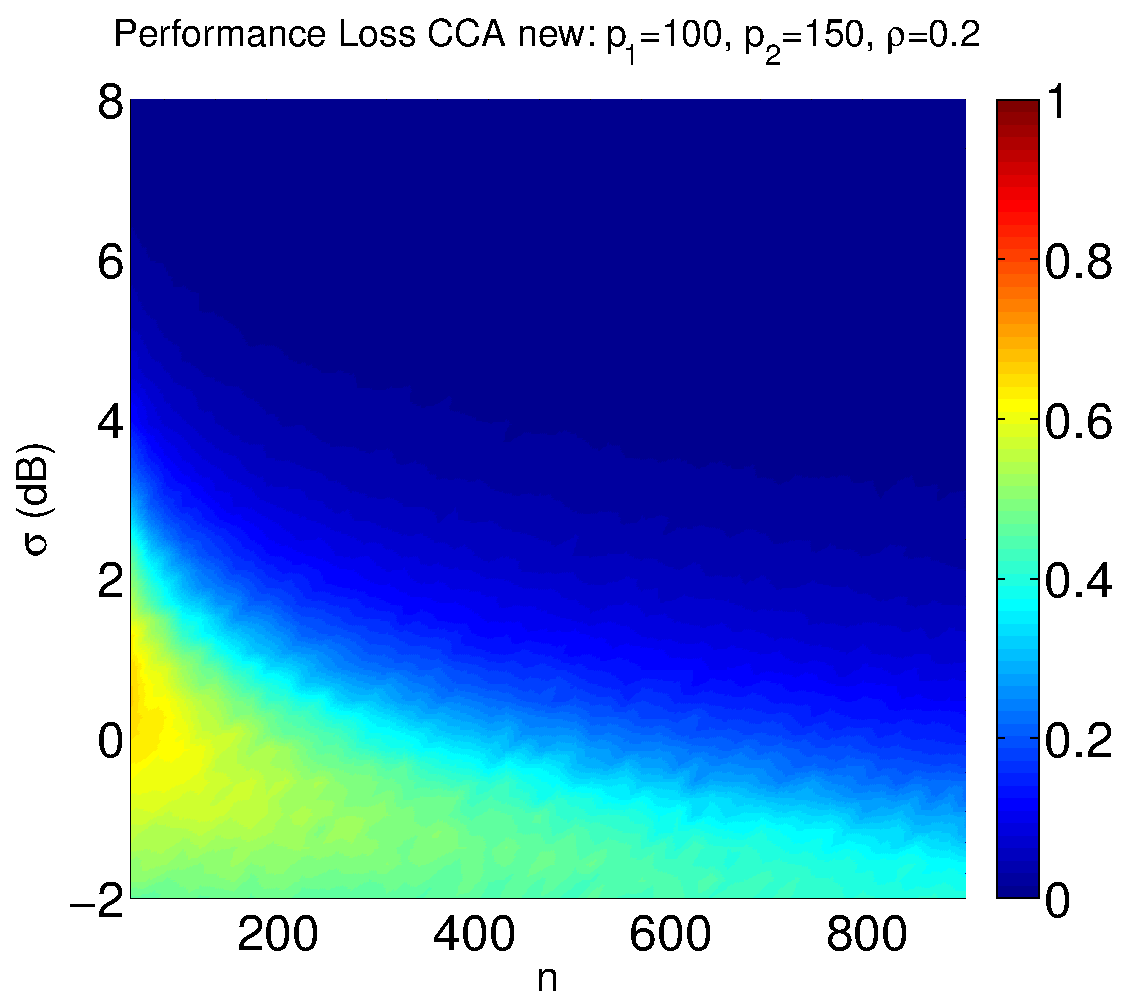
\includegraphics[width=4in]{figures/pl_cca_new_small.pdf}
%\end{figure}


%\begin{figure} 
%\centering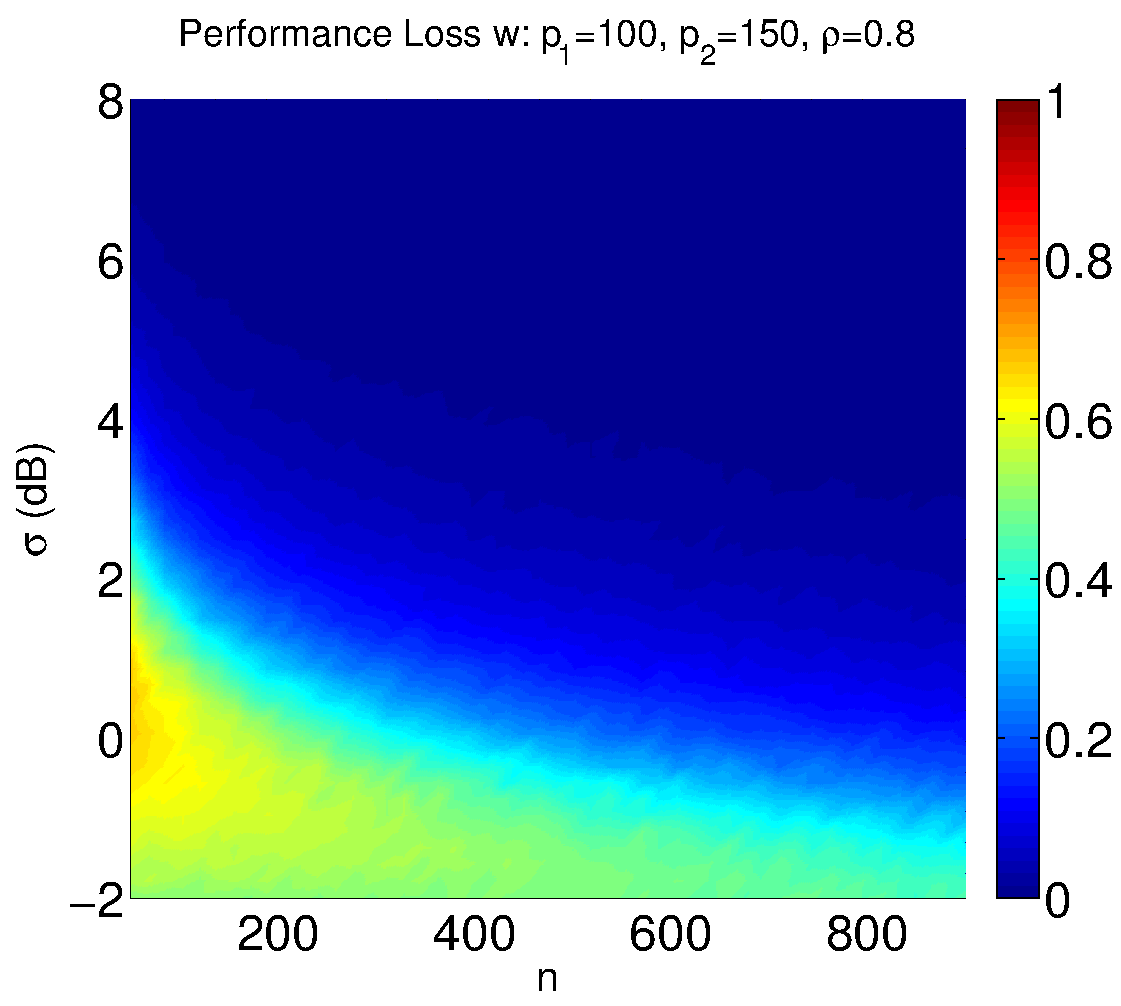
\includegraphics[width=4in]{figures/pl_w_large.pdf}
%\end{figure}

%\begin{figure} 
%\centering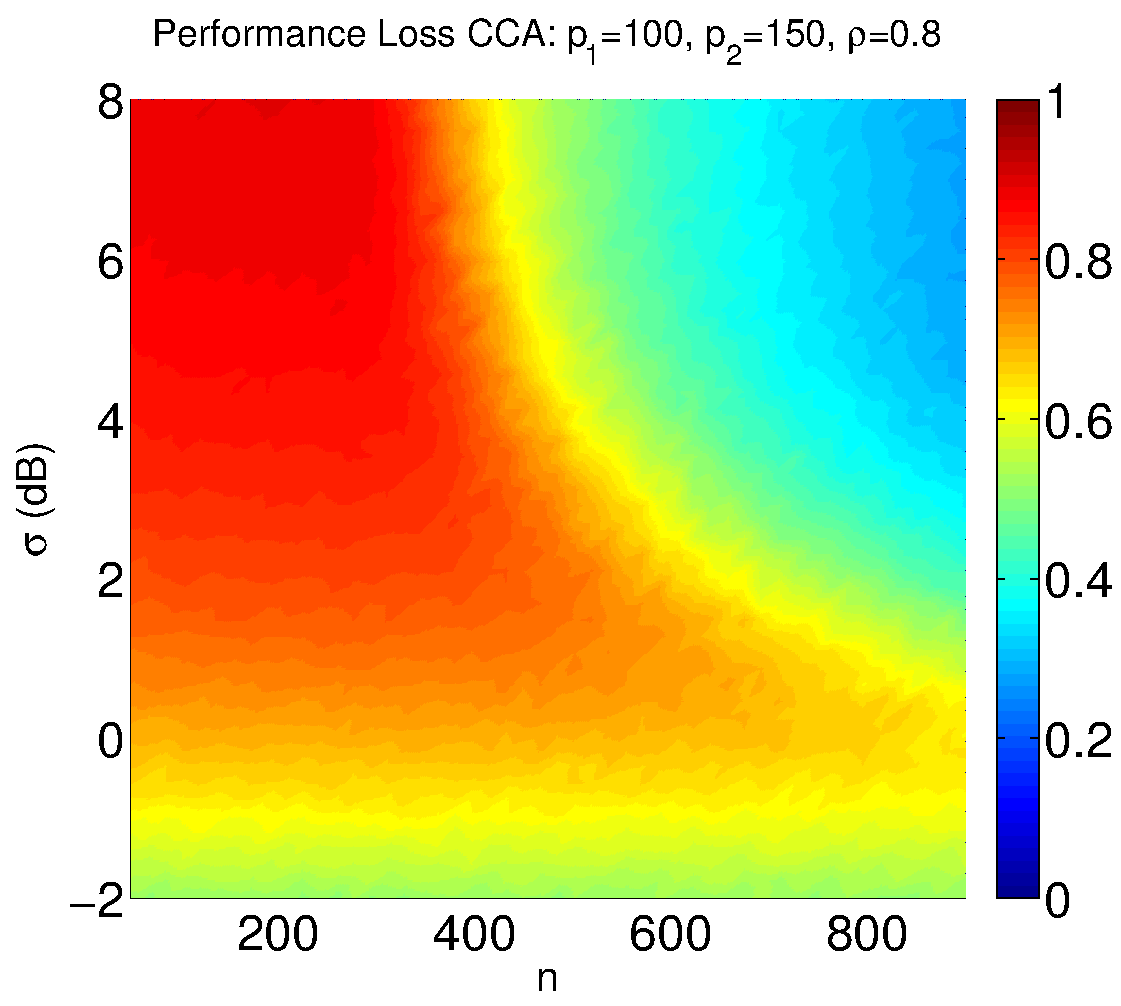
\includegraphics[width=4in]{figures/pl_cca_large.pdf}
%\end{figure}

%\begin{figure} 
%\centering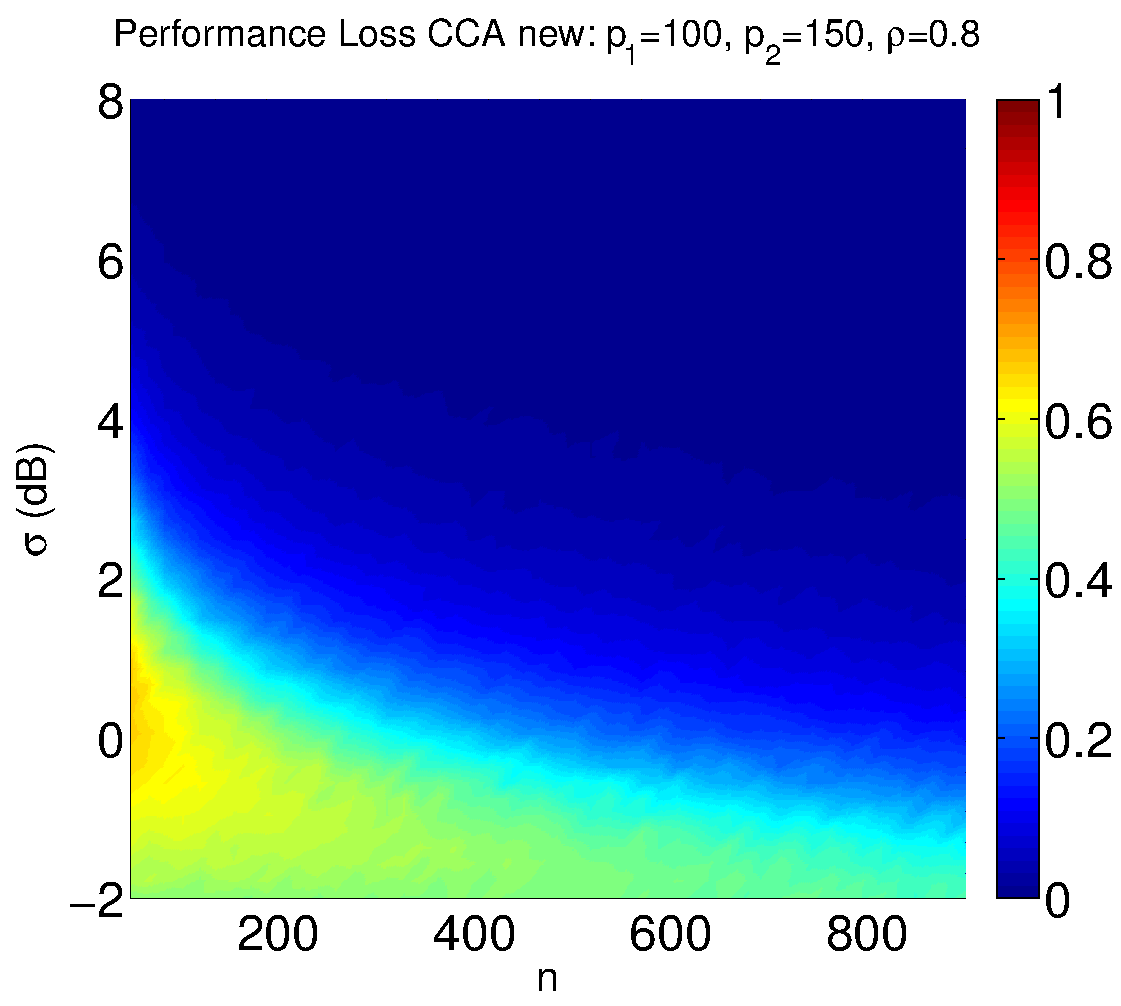
\includegraphics[width=4in]{figures/pl_cca_new_large.pdf}
%\end{figure}


\chapter{Regularized CCA (RCCA)}\label{sec:rcca}
As mentioned in Chapter \ref{sec:cca}, in the sample starved regime where the number of
samples is less than the combined dimensions of the datasets, it is common to
regularize CCA. By adding a penalty to the $\ell_2$ norm of the canonical vectors in the
CCA objective function we arrive at a regularized version of CCA (RCCA). This optimization
also has a closed form solution that is dependent on the SVD of a matrix involving the
covariance matrices of our data. However, unlike CCA, in the samples starved regime, this
solution is tractable as all matrix inverses are well defined. 

In this section we explore the performance of empirical RCCA, which has been previously
unexplored. We investigate the effect that the regularization parameter has on the
correlation estimate of returned by RCCA. Similar to the analysis conducted in Chapter
\ref{sec:cca}, we compute empirical distributions of this correlation estimate generated
from datasets that contain a correlated signal and from datasets that are purely noise. We
then explore using the correlation estimate to detect the presence of a signal.

Motivated by ICCA, we then develop an informative version of RCCA (IRCCA) that only uses
the informative components of the provided datasets. Finally, we explore the performance
of IRCCA and compare it to that of RCCA. We are particularly interested in how the
regularization parameter affects the distributions of the correlation estimate. We compare
using these correlation estimates to detect the presence of a target signal given two
correlated datasets. Our analysis shows that IRCCA exhibits many attractive behaviors not
exhibited by RCCA.

\section{Mathematical Formulation of RCCA}
RCCA uses the same data assumptions as CCA as described in Section \ref{sec:cca_form}. The
objective is still to find the canonical vectors $\xI$ and $\xII$ that maximize the correlation
between the canonical variates $\wI=\xI^H\yI$ and $\wII=\xII^H\yII$. RCCA introduces a
regularization parameter, $\eta$, that penalizes the $\ell_2$ norm of the canonical
vectors. Formally, the RCCA optimization problem is
\begin{equation}\label{eq:rcca_opt1}
  \begin{aligned}
    &\argmax_{\xI,\xII}&&\rho = E[\wI\wII]\\
    & \text{subject to}&& E[\wI^2] + \eta \xI^H\xI\leq 1\\
    &&& E[\wI^2] + \eta \xII^H\xII\leq 1.\\
  \end{aligned}
\end{equation}
Note that in this formulation, we use the same regularization parameter for both canonical
vectors. One could relax this constraint and allow individual regularization parameters
$\eta_1$ and $\eta_2$ for each of the canonical vectors. 

Substituting the expressions for the canonical variates and correlation matrices used for
CCA, the RCCA optimization problems may be written
\begin{equation}\label{eq:rcca_opt2}
  \begin{aligned}
    &\argmax_{\xI,\xII}&&\rho = \xI^H\RIII\xII\\
    & \text{subject to}&& \xI^H\RI\xI + \eta \xI^H\xI\leq 1\\
    &&& \xII^H\RII\xII + \eta \xII^H\xII\leq 1.\\
  \end{aligned}
\end{equation}

However, since we are seeking to maximize $\rho$, we want to make the canonical vectors
have maximum norm so as to make $\rho$ as large as possible. Therefore, the inequality
constraint functions may be changed to constraint functions. 
\begin{equation}\label{eq:rcca_opt}
  \begin{aligned}
    &\argmax_{x_1,x_2}&&\rho = \xI^H\RIII\xII\\
    & \text{subject to}&& \xI^H\RI\xI + \eta \xI^H\xI= 1\\
    &&& \xII^H\RII\xII + \eta \xII^H\xII= 1.\\
  \end{aligned}
\end{equation}

The Lagrangian used to solve
(\ref{eq:rcca_opt}) is 
\begin{equation*}
  L(\xI,\xII,\lambda_1,\lambda_2) = \xI^H\RIII\xII - \lambda_1\left(\xI^H\left(\RI+\eta
      I_{d_1} \right)\xI  - 1 \right) - \lambda_2\left(\xII^H\left(\RII + \eta
      I_{d_2}\right)\xII - 1\right) 
\end{equation*}

To solve (\ref{eq:rcca_opt})
we take the partial derivatives of the Lagrangian and set them equal to zero. 
\beq\label{eq:rcca_partials}\ba
& 0 && = \RIII\xII -2\lambda_1\left(\RI + \eta I_{d_1}\right)\xI\\
& 0 && = \RIII^H\xI -2\lambda_2\left(\RII + \eta I_{d_2}\right)\xII.\\
\ea\eeq 
Similar to CCA, we immediately see that by multiplying the first equation in
(\ref{eq:rcca_partials}) by $\xI^H$ and the second by $\xII^H$ and applying the constraint
functions in (\ref{eq:rcca_opt}),
\be
\rho = 2\lambda_1 = 2\lambda_2.
\ee

Using this relationship and eliminating $\xII$ from  the partials in
(\ref{eq:rcca_partials}), results in the relationship
\beq\label{eq:rcca_x2}
\xII = \frac{1}{\rho}\left(\RII+\eta  I_{d_2}\right)^{-1}\RIII^H\xI.
\eeq
 and the eigenvalue system
\beq\label{eq:rcca_eigval}
\left(\RI+\eta I_{d_1}\right)^{-1}\RIII\left(\RII +\eta I_{d_2}\right)^{-1}\RIII^H\xI = 
\rho^2\xI
\eeq

Solving (\ref{eq:rcca_eigval}) for the eigenvector corresponding to the largest eigenvalue
solves (\ref{eq:rcca_opt}). Substituting this eigenvalue/eigenvector pair in
(\ref{eq:rcca_x2}) gives the complete solution $(\xI,\xII,\rho)$ for the canonical vectors
and maximum correlation coefficient of RCCA. Using a similarity transform as in the CCA
derivation, we may frame the eigen-system in (\ref{eq:rcca_eigval}) as an SVD
problem. Define $f=\left(\RI + \eta I_{d_1}\right)^{1/2}\xI$ and \\$g=\left(\RII + \eta
  I_{d_2}\right)^{1/2}\xII$. Then (\ref{eq:rcca_eigval}) may be written
\beq\label{eq:rcca_svd}
\left(\RI+\eta I_{d_1}\right)^{-1/2}\RIII\left(\RII +\eta
  I_{d_2}\right)^{-1}\RIII^H\left(\RI+\eta I_{d_1}\right)^{-1/2}\,f =\rho f. 
\eeq
Defining, $\Creg = \left(\RI+\eta I_{d_1}\right)^{-1/2}\RIII\left(\RII +\eta
  I_{d_2}\right)^{-1/2}$, (\ref{eq:rcca_svd}) 
\be
\Creg\Creg^Hf =\rho^2 f.
\ee

Therefore, $\rho$ is the largest singular value of $\Creg$ and $f$ is the corresponding
left singular vector. By a symmetry argument, $g$ is the corresponding right singular
vector. Let $FKG^H$ be the SVD of $\Creg$ where $F=[f_1,\dots,f_{d_1}]$,
$K\in\complex^{d_1\times d_2}=\diag(k_1,\dots,k_{\min\left(d_1,d_2\right)})$, and
$G=[g_1,\dots,g_{d_2}]$. The solution to RCCA is
\beq\label{eq:rcca_sol}\ba
    & \rho =k_1 \\
    & \xI=(\RI+\eta I_{d_1})^{-1/2}f_1 \\
    & \xII = (\RII+\eta I_{d_2})^{-1/2}g_1.\\
\ea\eeq

\section{Empirical RCCA}

The above derivation of a SVD solution to RCCA assumes that the covariance matrices $\RI$,
$\RII$, and $\RIII$ are all known. In many real world applications, this luxury is
generally not available and the covariance matrices must be estimated from training
data. In the same setup as empirical CCA in Section \ref{sec:emp_cca}, we assume that we
have access to $n$ observations from each dataset. We stack these observations in training
data matrices $Y_1=\left[\yI^{(1)},\dots,\yI^{(n)}\right]$ and
$Y_2=\left[\yII^{(1)},\dots,\yII^{(n)}\right]$. We form estimates of the covariance
matrices from the sample covariance matrices of these training data matrices as in
(\ref{eq:scm}). We substitute these estimates in the expression for $\Creg$ resulting in
\beq\label{eq:creghat}
 \Creghat =\left(\RIhat+\eta
  I_{d_1}\right)^{-1/2}\RIIIhat\left(\RIIhat +\eta I_{d_2}\right)^{-1/2} .
\eeq
Defining $\Creghat =\widehat{F}\widehat{K}\widehat{G}^H$ as the SVD of $\Creghat$, the
solution to empirical RCCA is 
\beq\label{eq:emp_rcca_sol}\ba
    & \widehat{\rho} = \widehat{k}_1 \\
    & \xIhat=(\RIhat+\eta I_{d_1})^{-1/2}\widehat{f}_1 \\
    & \xIIhat = (\RIIhat+\eta I_{d_2})^{-1/2}\widehat{g}_1.\\
\ea\eeq

In (\ref{eq:creghat}) and (\ref{eq:emp_rcca_sol}) we see the benefit of RCCA. We can now
compute $\Creghat$ as the matrix inverses will always be full rank, even in the sample
deficient regime when $n<d_1$ or $n<d_2$. In CCA, $\widehat{C}$ in (\ref{eq:cca_Chat}) was
not computable if the matrices $\RIhat$ or $\RIIhat$ were not invertible. Regularization
avoids this problem. 

We now simplify the computation of $\Creghat$ using the SVDs of the training data
matrices, $Y_1 = U_1\Sigma_1V_1^H$ and $Y_2= U_2\Sigma_2V_2$. Substituting these
decompositions in the sample covariance matrix estimates in (\ref{eq:scm}), we may write
$\Creghat$ in (\ref{eq:creghat}) as
\begin{equation}\label{eq:rcca_chat_decomp}
\Creghat = U_1(\Sigma_1\Sigma_1^H+ \eta
I_{d_1})^{-1/2}\Sigma_1V_1^HV_2\Sigma_2^H(\Sigma_2\Sigma_2^H + \eta I_{d_2})^{-1/2}U_2^H.
\end{equation}
This requires taking the inverse of diagonal matrices, which is computationally much more
desirable. Next we explore the previously unstudied performance of empirical RCCA.

\section{Performance of Empirical RCCA}

In this section, we explore the performance of empirical RCCA. We begin by describing the
simulation setup. We saw in the analysis of CCA that there is a sample poor regime where
CCA breaks down and a sample rich regime where CCA can be reliably used to detect the
presence of signals given correlated datasets. In RCCA, we have an additional parameter, $\eta$,
which controls the amount of regularization. We will be primarily interested in how
the regularization parameter affects the performance of RCCA. We note that as $n\to 0$,
RCCA approaches the CCA solution.

Similar to the performance analysis conducted for CCA, we will examine the largest
singular value of $\Creghat$, which we have denoted $\widehat{k}_1$. Specifically, we
will examine the empirical distribution of $\widehat{k}_1$ and how it changes with the
choice of $\eta$. We will again consider using the \naive detector that uses $\widehat{k}_1$
to detect the presence of a target signal given two correlated datasets. We explore the
AUC of such a detector, sweeping over the signal SNR and $\eta$ for a few fixed values of
the number of training samples, $n$.

\subsection{Simulation Setup}\label{sec:rcca_sim_setup}

We consider the same simulation data model used in the CCA performance analysis, which is
repeated here for reference.

\beq\label{eq:rcca_data_model1}\ba
\text{Noise:}\begin{cases}
\yI^{(i)}=\mathcal{N}\left(0,I_{d_1}\right) & \\
\yII^{(i)}=\mathcal{N}\left(0,I_{d_2}\right) & \\
\end{cases}
\text{Signal:}\begin{cases}
\yI^{(i)}=\sigma u_1 z_1^{(i)} + \mathcal{N}\left(0,I_{d_1}\right) & \\
\yII^{(i)}=\sigma u_2 z_2^{(i)} + \mathcal{N}\left(0,I_{d_2}\right) & \\
\end{cases}
\ea\eeq 
where $u_1\in\complex^{d_1}$ and $u_2\in\complex^{d_2}$ are unit norm signal
vectors, $\sigma>0$ is a SNR, and 
\be 
z^{(i)}=\left[\begin{array}{c}z_1^{(i)} \\
    z_2^{(i)}\end{array}\right]\sim \mathcal{N}\left(0,\left[\begin{array}{cc} 1 & \rho \\
      \rho & 1\end{array}\right]\right).  
\ee 
All additive Gaussian noise terms are independent. We note that in this setup the SNR,
$\sigma$, is the same for both datasets. This would usually not be the case and we could
run these simulations using a $\sigma$ unique to each dataset, however, since we are
adding the additional regularization parameter $\eta$, we wish to reduce the number of
parameters in the simulation.

For $i=1,\dots,n$ we produce $n$ samples for each dataset under both the signal and noise
model in (\ref{eq:rcca_data_model1}) to produce four datasets $Y_1^{\text{noise}}$,
$Y_2^{\text{noise}}$, $Y_1^{\text{signal}}$, and $Y_2^{\text{signal}}$. We then take the
data SVD of each dataset and use these data SVDs to form two copies
$\Creghat^{\text{noise}}$ and $\Creghat^{\text{signal}}$ as in
(\ref{eq:rcca_chat_decomp}). We then take the leading singular value of both
$\Creghat^{\text{noise}}$ and $\Creghat^{\text{signal}}$, resulting in two top singular
values estimating the maximum correlation, $\widehat{\rho}_{\text{reg}}^{\text{noise}}$
and $\widehat{\rho}_{\text{reg}}^{\text{signal}}$. This is repeated for multiple trials,
where each trial generates new datasets using different signal vectors $u_1$ and $u_2$,
new $z$, and new additive noise. This gives an empirical distribution of
$\widehat{\rho}_{\text{reg}}^{\text{noise}}$ and
$\widehat{\rho}_{\text{reg}}^{\text{signal}}$, the correlation estimates formed from
$\Creghat^{\text{noise}}$ and $\Creghat^{\text{signal}}$.

\subsection{Distribution of $\widehat{\rho}$}

We first explore the effect that the regularization parameter, $\eta$ has on the top
singular value, $\widehat{k}_1$ of $\Creghat^{\text{noise}}$ and
$\Creghat^{\text{signal}}$. Recall that the correlation coefficient estimate is
$\widehat{\rho} = \widehat{k}_1$ so we use these interchangeably. For a fixed value of the
number of samples, $n$, and SNR, $\sigma$, we compute the empirical distribution of
$\widehat{k}_1$ as described in Section \ref{sec:rcca_sim_setup} for multiple values of
the $\eta$. Figures \ref{fig:rcca_errorbars_low_snr} and \ref{fig:rcca_errorbars_high_snr}
plots these empirical distributions for four values of $n$ for an SNR of 0 dB and 3 dB,
respectively.

\begin{figure}[h!]
\subfigure[$n=50$]{
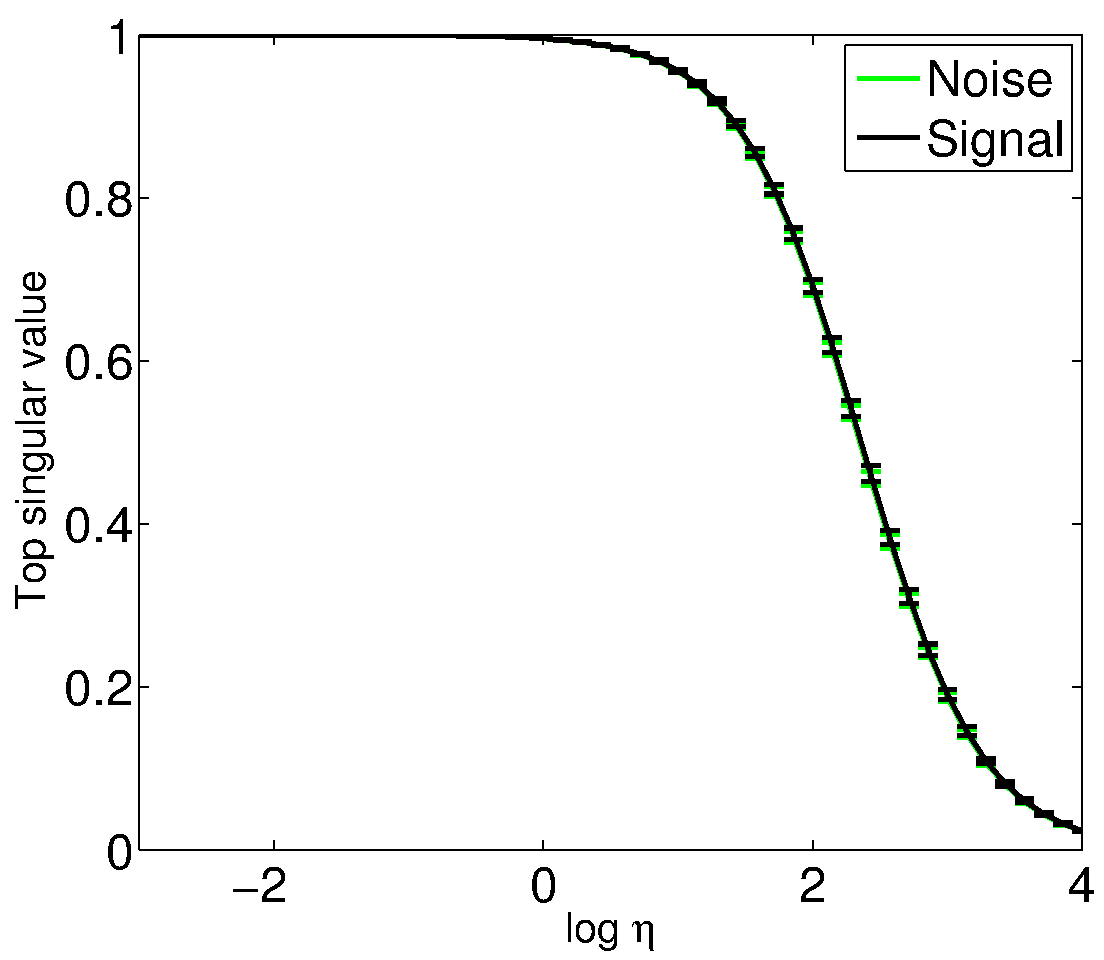
\includegraphics[width=\figwidth]{figures/rcca_errorbars_low_snr_n_50.pdf} 
} 
\subfigure[$n=150$]{
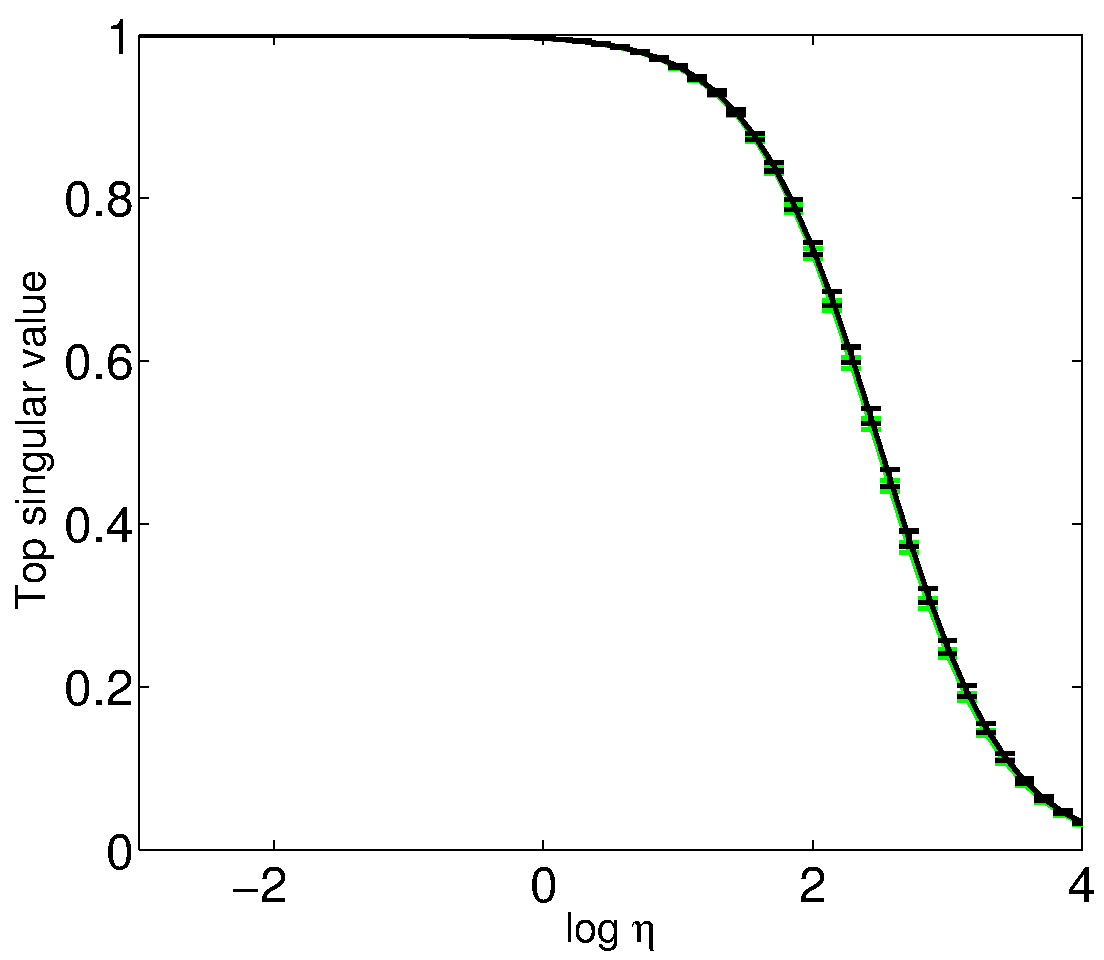
\includegraphics[width=\figwidth]{figures/rcca_errorbars_low_snr_n_150.pdf} 
} 
\subfigure[$n=300$]{
\includegraphics[width=\figwidth]{figures/rcca_errorbars_low_snr_n_300.pdf} 
} 
\subfigure[$n=600$]{
\includegraphics[width=\figwidth]{figures/rcca_errorbars_low_snr_n_600.pdf} 
} 
\caption{Empirical distribution of the top singular value of $\Creghat$ in
  (\ref{eq:creghat}) for both noise and signal data models in
  (\ref{eq:rcca_data_model1}). Simulations were conducted using $d_1=200$, $d_2=150$,
  $\rho=0.9$, and $\sigma=0$ dB. Results are shown for four values of $n$. The top
  singular value was computed for 500 trials. The mean top singular value is plotted with
  $\pm$ one standard deviation errorbars. The distribution of the top singular value of the
  noise distribution is plotted in green and that of the signal distribution is plotted in
  black.}
\label{fig:rcca_errorbars_low_snr}
\end{figure}

\begin{figure}[h!]
\subfigure[$n=50$]{
\includegraphics[width=\figwidth]{figures/rcca_errorbars_high_snr_n_50.pdf} 
} 
\subfigure[$n=150$]{
\includegraphics[width=\figwidth]{figures/rcca_errorbars_high_snr_n_150.pdf} 
} 
\subfigure[$n=300$]{
\includegraphics[width=\figwidth]{figures/rcca_errorbars_high_snr_n_300.pdf} 
} 
\subfigure[$n=600$]{
\includegraphics[width=\figwidth]{figures/rcca_errorbars_high_snr_n_600.pdf} 
} 
\caption{Empirical distribution of the top singular value of $\Creghat$ in
  (\ref{eq:creghat}) for both noise and signal data models in
  (\ref{eq:rcca_data_model1}). Simulations were conducted using $d_1=200$, $d_2=150$,
  $\rho=0.9$, and $\sigma=3$ dB. Results are shown for four values of $n$. The top singular
  value was computed for 500 trials. The mean top singular value is plotted with $\pm$ one
  standard deviation errorbars. The distribution of the top singular value of the noise
  distribution is plotted in green and that of the signal distribution is plotted in
  black.}
\label{fig:rcca_errorbars_high_snr}
\end{figure}

These figures present a number of interesting results. First, we see that for each value
of $n$, when $\eta$ is small, the value of $\widehat{\rho}$ is large under both the signal
and noise distribution. It is undesirable for $\widehat{\rho}$ to be large under the noise
distribution as this indicates a strong correlation between the datasets while in fact,
there is no correlation. 

As is expected, the noise and signal empirical distributions separate more at a larger
SNR. This is more evident at larger value of $n$. This behavior is very intuitive as one
would hope that more samples and a larger SNR would yield statistically different
distributions. A visual inspection of the distributions show that when $\sigma=3$ dB, the
distributions are completely separable when $n=600$. In fact, for all value of $n$, it
appears that the distributions separate more for larger value of $\eta$. 

When $\eta$ is increased, the value of $\widehat{\rho}$ decreases rapidly. In all eight
figures, there seems to be a phase transition in $\eta$. For low value of $\eta$,
$\widehat{\rho}$ remains relatively constant. For values of $\eta$ above a critical value,
the value of $\widehat{\rho}$ begins to decrease rapidly. Since $\eta$ controls the
magnitude of the canonical vectors, larger $\eta$ will force the canonical vectors to have
a small norm. In this regime of large $\eta$, it is possible that we are sacrificing the
accuracy of the canonical vectors to achieve better separability between the empirical
distributions of $\widehat{\rho}$. More experiments investigating the behavior of the
singular vectors are most certainly necessary. 

\subsection{Detection Based on $\widehat{\rho}$}

We next explore how well the noise and signal empirical distributions of $\widehat{\rho}$
separate. Similar to the CCA analysis, we consider the \naive detector that thresholds
based on $\rho$ to detect signal versus noise given two possibly correlated datasets. Given
the two empirical distributions for the noise and signal datasets, we construct an
empirical ROC curve. We measure the detection power of such a detector by computing the
area under the empirical ROC curve (AUC) as was done in the analysis of CCA. Figure
\ref{fig:rcca_auc_heatmap} plots the empirical AUC for such a detector for four different
values of $n$ while sweeping over both $\sigma$ and $\eta$.

\begin{figure}[h!]
\subfigure[$n=50$]{
\includegraphics[width=\figwidth]{figures/rcca_auc_heatmap_n_50.pdf} 
} 
\subfigure[$n=150$]{
\includegraphics[width=\figwidth]{figures/rcca_auc_heatmap_n_150.pdf} 
} 
\subfigure[$n=300$]{
\includegraphics[width=\figwidth]{figures/rcca_auc_heatmap_n_300.pdf} 
} 
\subfigure[$n=600$]{
\includegraphics[width=\figwidth]{figures/rcca_auc_heatmap_n_600.pdf} 
} 
\caption{Empirical AUC of the detector based on the top singular value of $\Creghat$ in
  (\ref{eq:creghat}) based on the data models in (\ref{eq:rcca_data_model1}). Simulations
  were conducted using $d_1=200$, $d_2=150$, $\rho=0.9$, and 500 trials. Results are
  shown for 4 values of $n$. In each figure, the AUC is plotted for multiple combinations
  of $\sigma$ and $\eta$.}
\label{fig:rcca_auc_heatmap}
\end{figure}

First we see that in the sample poor regime when $n=50$, RCCA allows detection of the
target signal. Compared to Figure \ref{fig:cca_auc_heatmap}, RCCA drastically increases
detection ability in this low sample regime. There is a critical value of SNR under which
the target signal may no longer be reliably detected. The performance of such a detector
in this sample poor regime seems to be unaffected by the choice of regularization
parameter.

When increasing the number of samples to $n=150$, we see an interesting phenomena. With
more samples, we seem to be able to tolerate a slightly lower value of $\sigma$ to achieve
the same performance as the detector using $n=50$ training samples. This is intuitive and
desirable. We are still operating in the regime of $n<d_1+d_2$ where CCA breaks
down. However, RCCA is now able to reliably detect the presence of signal. The phenomena
arises when considering the affect of $\eta$. We see that if we allow $\eta$ to be very
large, we can increase in the detection ability of the \naive detector based on
$\widehat{k}_1$. Again, we may be sacrificing the accuracy of the canonical vectors to
gain this increased detection ability.

An extremely interesting phenomena arises when increasing $n$ to 300. In this regime, we
are still have $n<d_1+d_2$ but we have enough samples that $\RIhat$ and $\RIIhat$ are both
full rank. We now see a large portion of the heatmap indicate that the detector has no
detection ability. Unlike the detectors using less samples, this detector must have a
large enough regularization parameter to have useful detection ability. Similar to the
detector using $n=150$ samples, if we allow $\eta$ to increase large enough, we can
tolerate a much smaller SNR and still achieve good detection ability. The behavior of RCCA
seems to be highly dependent on both the number of samples and the value of the
regularization parameter. This is very undesirable.

Finally, when we increase $n$ to 600, we return to a similar behavior when $n=150$. For
lower values of $\eta$, we seem to have approximately the same performance as the
detectors using $n=50$ and $n=150$ samples. This is very undesirable as the more training
samples that we have, the better performance we should achieve. Again we see that by
increasing $\eta$ large enough, we can tolerate a much smaller SNR to achieve the same AUC
performance. Future work describing how the regularization parameter affects the canonical
vectors is of utmost importance.

\section{Informative RCCA (IRCCA)}

In this section, we apply the ideas of informative CCA to regularized CCA. As seen in the
previous section, the performance of RCCA is irregular and highly dependent on the choice
of the regularization parameter and number of samples. We first derive an informative
version of RCCA (IRCCA) and show, through numerical simulations, that it has a more
consistent performance that is not dependent on the regularization parameter and which
improves with more training samples. We compare the performance of RCCA and IRCCA when
used for signal detection and highlight parameter regimes where each works best.

\subsection{IRCCA Derivation}

We begin by recalling the singular value decompositions of the data matrices, $Y_1 =
U_1\Sigma_1V_1^H$ and $Y_2= U_2\Sigma_2V_2$.  Examining (\ref{eq:rcca_chat_decomp}), we
observe that the estimate for the maximum correlation between the datasets is
\begin{equation}\label{eq:rcca_rhohat}
\widehat{\rho} = \sigma_1(\Creghat) = \sigma_1\left((\Sigma_1\Sigma_1^H+\eta
I_{d_1})^{-1/2}\Sigma_1V_1^HV_2\Sigma_2^H(\Sigma_2\Sigma_2^H + \eta
I_{d_2})^{-1/2}\right).
\end{equation}
From this expression, it is clear that RCCA relies on the matrix product $V_1^HV_2$. This
term most likely causes the irregularity in the performance of RCCA as it broke the
performance of CCA in the sample starved regime. Following the guidance in Proposition
\ref{prop:raj}, we only want to use the singular vectors of $V_1$ and $V_2$ that are
informative. In low-rank systems, this proposition tells us that many of these right
singular vectors are uninformative and using them would only introduce additional noise
into the algorithm. Following the approach in CCA, we define the trimmed data matrices
\be\ba
&\widetilde{\Sigma}_1=\Sigma_1(1:r_1,1:r_1) &&\widetilde{\Sigma}_2=\Sigma_2(1:r_2,1:r_2)\\
&\widetilde{U}_1=U_1(:,1:r_1) &&\widetilde{U}_2=U_2(:,1:r_2)\\
&\widetilde{V}_1=V_1(:,1:r_1) &&\widetilde{V}_2=V_2(:,1:r_2)\\
\ea\ee where $r_1$ and $r_2$ are the number of informative components computed by
Proposition \ref{prop:raj} in the first and second datasets, respectively.

Using these trimmed data matrices results in an informative RCCA (IRCCA) algorithm. We
first construct
\beq\label{eq:cregtil}
\Cregtil = \widetilde{U}_1(\widetilde{\Sigma}_1\widetilde{\Sigma}_1^H+ \eta
I_{r_1})^{-1/2}\widetilde{\Sigma}_1\widetilde{V}_1^H\widetilde{V}_2\widetilde{\Sigma}_2^H
(\widetilde{\Sigma}_2\widetilde{\Sigma}_2^H + \eta I_{r_2})^{-1/2}\widetilde{U}_2^H 
\eeq
and then take the SVD $\Cregtil = \widetilde{F}\widetilde{K}\widetilde{G}^H$. The IRCCA
canonical vectors and correlation coefficient estimates are
\be\ba
& \widetilde{\rho} = \widetilde{k}_1\\
& \widetilde{x}_1 = (\RIhat+\eta I_{d_1})^{-1/2}\widetilde{f}_1\\
& \widetilde{x}_2 = (\RIIhat+\eta I_{d_2})^{-1/2}\widetilde{g}_1.\\
\ea\ee

\subsection{Numerical Simulations}

We use the same simulation setup as in RCCA above, generating $n$ samples from
(\ref{eq:rcca_data_model1}) to form $Y_1^{\text{noise}}$, $Y_2^{\text{noise}}$,
$Y_1^{\text{signal}}$, and $Y_2^{\text{signal}}$. We use these training data matrices to
compute $\Cregtil^{\text{noise}}$ and $\Cregtil^{\text{signal}}$ as in
(\ref{eq:cregtil}). For two values of $\sigma$, figures \ref{fig:rcca_errorbars_low_snr}
and \ref{fig:rcca_errorbars_high_snr} plot the empirical distributions of the IRCCA
correlation estimate, $\widetilde{\rho}$, generated from the SVD of
$\Cregtil^{\text{noise}}$ and $\Cregtil^{\text{signal}}$. The RCCA correlation estimate,
$\widehat{\rho}$, is also plotted for comparison.

\begin{figure}[h!]
\subfigure[$n=50$]{
\includegraphics[width=\figwidth]{figures/ircca_errorbars_low_snr_n_50.pdf} 
} 
\subfigure[$n=150$]{
\includegraphics[width=\figwidth]{figures/ircca_errorbars_low_snr_n_150.pdf} 
} 
\subfigure[$n=300$]{
\includegraphics[width=\figwidth]{figures/ircca_errorbars_low_snr_n_300.pdf} 
} 
\subfigure[$n=600$]{
\includegraphics[width=\figwidth]{figures/ircca_errorbars_low_snr_n_600.pdf} 
} 
\caption{Empirical distribution of the top singular value of $\Cregtil$ in
  (\ref{eq:cregtil}) for both noise and signal data models in
  (\ref{eq:rcca_data_model1}). Simulations were conducted using $d_1=200$, $d_2=150$,
  $\rho=0.9$, and $\sigma=0$ dB. Results are shown for four values of $n$. The top
  singular value was computed for 500 trials. The mean top singular value is plotted with
  $\pm$ one standard deviation errorbars. The figure plots the distribution of the top
  singular value of the RCCA noise distribution (green), RCCA signal distribution (black),
  IRCCA noise distribution (blue), and IRCCA signal distribution (red).}
\label{fig:rcca_errorbars_low_snr}
\end{figure}

\begin{figure}[h!]
\subfigure[$n=50$]{
\includegraphics[width=\figwidth]{figures/ircca_errorbars_high_snr_n_50.pdf} 
} 
\subfigure[$n=150$]{
\includegraphics[width=\figwidth]{figures/ircca_errorbars_high_snr_n_150.pdf} 
} 
\subfigure[$n=300$]{
\includegraphics[width=\figwidth]{figures/ircca_errorbars_high_snr_n_300.pdf} 
} 
\subfigure[$n=600$]{
\includegraphics[width=\figwidth]{figures/ircca_errorbars_high_snr_n_600.pdf} 
} 
\caption{Empirical distribution of the top singular value of $\Creghat$ in
  (\ref{eq:creghat}) for both noise and signal data models in
  (\ref{eq:rcca_data_model1}). Simulations were conducted using $d_1=200$, $d_2=150$,
  $\rho=0.9$, and $\sigma=3$ dB. Results are shown for four values of $n$. The top
  singular value was computed for 500 trials. The mean top singular value is plotted with
  $\pm$ one standard deviation errorbars. The figures plots the distribution of the top
  singular value of the RCCA noise distribution (green), RCCA signal distribution (black),
  IRCCA noise distribution (blue), and IRCCA signal distribution (red).}
\label{fig:rcca_errorbars_high_snr}
\end{figure}

Figures \ref{fig:rcca_errorbars_low_snr} and \ref{fig:rcca_errorbars_high_snr} demonstrate
that the correlation estimate of IRCCA has many desirable properties. First, for both
values of SNR presented, the correlation estimate of the noise distribution decreases with
increased training samples. The datasets under the noise distribution are not correlated
and so it is desirable that IRCCA returns a correlation estimate close to zero and that
IRCCA becomes more confident that there is no correlation when more training samples are
available. 

Second, for both values of SNR presented, the IRCCA correlation estimate for the signal
distribution increases with more training samples. The datasets under the signal
distribution are highly correlated ($\rho=0.9$) and so it is desirable that IRCCA becomes
more confident that there is a correlation when more training samples are available. This
estimated correlation distribution is also larger for the larger value of SNR in
Figure \ref{fig:rcca_errorbars_high_snr}. It is also very desirable that IRCCA becomes more
confident that there is correlation when the SNR of the low-rank signal becomes stronger. 

Similar to the performance of RCCA, IRCCA also seems to exhibit a phase transition in the
correlation estimate that is dependent on $\eta$. For smaller values of $\eta$, the value
of $\widetilde{\rho}$ is constant for both the signal and noise data model. However, once
$\eta$ is increased past a certain threshold, the value of $\widetilde{\rho}$ decreases
rapidly. As suggested in the discussion of the performance of RCCA, we speculate that this
is due to overfitting and that the canonical vectors may be very inaccurate. Future work
examining the accuracy of the canonical vectors of both RCCA and IRCCA is paramount for
the thesis.

Visually, IRCCA seems to do a better job at separating the noise and signal distributions
for lower values of $n$ and for lower values of $\sigma$. However, visually examining
these distributions does not give an indication of how well we can distinguish between the
two. Instead, we perform the same AUC analysis as done in the RCCA analysis, using
$\widetilde{\rho}$ as the statistic for a \naive detector. We compute the empirical ROC
curve from the empirical distributions and then compute the AUC to determine the detection
ability of the detector. Figures \ref{fig:ircca_auc_heatmap1} and
\ref{fig:ircca_auc_heatmap2} show the AUC for the IRCCA detector for many values of $\eta$
and $\sigma$. The difference plot between IRCCA and RCCA is plotted for
comparison. Positive values represent that IRCCA does better. Negative values represent
that RCCA does better.

\begin{figure}[h!]
\subfigure[IRCCA, $n=50$]{
\includegraphics[width=\figwidth]{figures/ircca_auc_heatmap_n_50.pdf} 
} 
\subfigure[RCCA Difference, $n=50$]{
\includegraphics[width=\figwidth]{figures/ircca_auc_heatmap_diff_n_50.pdf} 
} 
\subfigure[IRCCA, $n=150$]{
\includegraphics[width=\figwidth]{figures/ircca_auc_heatmap_n_150.pdf} 
} 
\subfigure[RCCA Difference, $n=150$]{
\includegraphics[width=\figwidth]{figures/ircca_auc_heatmap_diff_n_150.pdf} 
} 
\caption{Empirical AUC of the detector based on the top singular value of $\Cregtil$ in
  (\ref{eq:creghat}) based on the data models in (\ref{eq:rcca_data_model1}). Simulations
  were conducted using $d_1=200$, $d_2=150$, $\rho=0.9$, and 500 trials. Results are shown
  for IRCCA and the difference between IRCCA and RCCA for $n=50,150$. In each figure, the
  AUC is plotted for multiple combinations of $\sigma$ and $\eta$. In the difference
  plots, positive values indicate that IRCCA does better and negative values indicate that
  RCCA does better.}
\label{fig:ircca_auc_heatmap1}
\end{figure}


\begin{figure}[h!]
\subfigure[IRCCA, $n=300$]{
\includegraphics[width=\figwidth]{figures/ircca_auc_heatmap_n_300.pdf} 
} 
\subfigure[RCCA Difference, $n=300$]{
  \includegraphics[width=\figwidth]{figures/ircca_auc_heatmap_diff_n_300.pdf} 
} 
\subfigure[IRCCA, $n=600$]{
  \includegraphics[width=\figwidth]{figures/ircca_auc_heatmap_n_600.pdf} 
} 
\subfigure[RCCA Difference, $n=600$]{
\includegraphics[width=\figwidth]{figures/ircca_auc_heatmap_diff_n_600.pdf} 
} 
\caption{Empirical AUC of the detector based on the top singular value of $\Cregtil$ in
  (\ref{eq:creghat}) based on the data models in (\ref{eq:rcca_data_model1}). Simulations
  were conducted using $d_1=200$, $d_2=150$, $\rho=0.9$, and 500 trials. Results are shown for IRCCA and
  the difference between IRCCA and RCCA for $n=300,600$. In each figure, the AUC is plotted
  for multiple combinations of $\sigma$ and $\eta$. In the difference plots, positive
  values indicate that IRCCA does better and negative values indicate that RCCA does
  better.}
\label{fig:ircca_auc_heatmap2}
\end{figure}

Figures \ref{fig:ircca_auc_heatmap1} and \ref{fig:ircca_auc_heatmap2} immediately show
that the performance of IRCCA is not affected by the regularization parameter,
$\eta$. This may be a false result because we are only considering a rank-1
signal. However, compared to the rank-1 performance of RCCA, this is a very desirable
property of IRCCA because the performance is much more predictable. Second, as the
number of training samples increases, the performance of IRCCA improves. For larger values
of $n$, IRCCA can tolerate a lower SNR, $\sigma$, and still achieve the same performance
as that of an IRCCA detector using less samples. This is a much desired improvement over
RCCA.

Comparing the difference plots between IRCCA and RCCA, we see that when $n=50$, in the
regime of medium SNR ($\sigma\approx 0$ dB) RCCA achieves better performance than
IRCCA. In the high SNR and low SNR regimes, the detectors essentially achieve the same
performance. For this value of $n$, the sample covariance matrices are ill-determined and
RCCA is necessary to prevent inverting singular matrices. It seems fitting that RCCA
achieves its best performance in this regime. 

For $n=150,300,600$, the difference plots between IRCCA and RCCA exhibit the same
behavior. For low values of $\eta$, there is a regime in which IRCCA achieves a
performance gain over RCCA. This region is quite large for $n=300$ and the performance
gain is very large for $n=300$ and $n=600$. In this low $\eta$ regime, IRCCA can achieve
the same performance as RCCA while tolerating a lower SNR. For larger values of $\eta$,
there is a regime where RCCA outperforms IRCCA. This performance gain is on the order of
0.1 AUC for all values of $n$. As previously described, we believe that in this regime of
large $\eta$, we sacrifice the accuracy of the canonical vectors and overfit the
problem. Therefore, the performance gain in this regime may not be real. Further
investigation into the accuracy of the canonical vectors of IRCCA and CCA is primary work
for the thesis.

\section{Limiting as $\eta\to\infty$}

In the previous section, the performance of RCCA improves as $\eta$ increases. This seems
contradict the notion in many regularized algorithms that over regularizing will decrease
performance. Ideally, there is an optimal regularization parameter. In this section, we let
$\eta\to\infty$ to derive a limit version of RCCA, which we call LRCCA. We compare the
performance of LRCCA to ICCA and RCCA. 

We begin with $\Creghat$ as defined in (\ref{eq:rcca_chat_decomp}). Define
$\widetilde{U}_1 = U_1(:,1:\min(d_1,n))$, $\widetilde{U}_2 = U_2(:,1:\min(d_2,n))$,
$\widetilde{V}_1 = V_1(:,1:\min(d_1,n))$, and $\widetilde{V}_2 =
V_2(:,1:\min(d_2,n))$. Then 
\begin{equation}
  \Creghat = \widetilde{U}_1\diag\left(\frac{\sigma_{1i}}{\sqrt{\sigma_{1i}^2 +
        \eta}}\right)\widetilde{V}_1^H\widetilde{V}_2
  \diag\left(\frac{\sigma_{2i}}{\sigma_{2i}^2 +\eta}\right)\widetilde{U}_2^H. 
\end{equation}
The matrix $\Creghat$ is a function of the regularization parameter, $\eta$. We would like
to examine the limiting matrix of $\Creghat$ as $\eta\to\infty$. As seen above, $\eta$
only comes into play in the two diagonal matrices and we begin by deriving the limit of
these matrices as $\eta\to\infty$. 

Clearly, as $\eta\to\infty$, these matrices become the zero matrix. However, the ratio of
the diagonal entries is what we care about. Let us consider just this.
\begin{equation*}
\lim_{\eta\to\infty} \frac{\sqrt{\frac{\sigma_{1i}^2}{\sigma_{1i}^2 +
      \eta}}}{\sqrt{\frac{\sigma_{1(i+1)}^2}{\sigma_{1(i+1)}^2 + \eta}}} =
\lim_{\eta\to\infty}
\sqrt{\frac{\sigma_{1i}^2(\sigma_{1(i+1)}^2+\eta)}{\sigma_{1(i+1)}^2(\sigma_{1i}^2 +
  \eta)} } = \frac{\sigma_{1i}}{\sigma_{1(i+1)}}
\end{equation*}
Thus, as $\eta\to\infty$, the entries along diagonal matrix approaches the ratio between
the original singular values, or a scaled version of the original singular value matrix
$\Sigma_1$ and $\Sigma_2$. As the scaling of this matrix will not affect the canonical
vectors, we can simply ignore it. Let $\widetilde{\Sigma}_1 =
\Sigma_1(1:\min(d_1,n),1:\min(d_1,n))$, and $\widetilde{\Sigma}_2 =
\Sigma_2(1:\min(d_2,n):,1:\min(d_2,n))$. Then
\begin{equation*}
  \widehat{C}_{\text{lrcca}}= \lim_{\eta\to\infty}\Creghat =
  \widetilde{U}_1\widetilde{\Sigma}_1\widetilde{V}_1^H\widetilde{V}_2\widetilde{\Sigma}_2\widetilde{U}_2^H
  = Y_1Y_2^H.
\end{equation*}
Let $\widehat{C}_{\text{lrcca}} = \widehat{F}\widehat{K}\widehat{G}^H$ be the SVD of
$\widehat{C}_{\text{lrcca}}$. Then the canonical correlation and canonical vectors are
\begin{equation}
\ba
& \widehat{\rho} = \widehat{k}_1\\
& \xIhat = f\\
& \xIIhat = g\\
\ea
\end{equation}

\section{Conclusion}

In this section, we examined the performance of regularized CCA. Regularization allows for
a tractable solution, even in the sample poor regime when the number of samples is less
than the dimension of the datasets. We first examined the behavior of the canonical
correlation coefficient estimate returned by empirical RCCA, which uses sample covariance
estimates for the unknown covariance matrices. We observed that the correlation estimate
largely affected by the choice of regularization parameter. In the case when the datasets
were generated only from Gaussian noise, RCCA sill reported a strong correlation between
the datasets. Using this correlation estimate to detect the presence of a target signal
was possible with RCCA. However, the performance of such an RCCA detector is very
irregular. The choice of $\eta$ highly affects the performance while more samples does not
necessarily lead to better detection performance. RCCA seemed to work best when used in
the sample poor regime that motivated its use. For large values of the regularization
parameter, we observed an increase in detection ability. However, evidenced by the phase
transition in the distribution of the correlation estimate, we believe this to be a
consequence of overfitting. Further work investigating the accuracy of the canonical vector
estimates is left to the thesis.

In the spirit of ICCA, we developed an informative version of RCCA called IRCCA. By
trimming the data SVDs we only use the informative components present in the data. IRCCA
exhibits some very beneficial properties. The value of the IRCCA correlation estimate
increases with the number of training samples when there is a correlated signal present
and decreases with the number of training samples when there is no correlated signal
present in the datasets. IRCCA may also be susceptible to overfitting as the correlation
estimate also exhibited a phase transition for large values of $\eta$. Using the
correlation estimate of IRCCA for signal detection provided encouraging results. The
performance of such a detector seems to be invariant to the choice of $\eta$. Unlike the
RCCA detector, the performance of IRCCA increases with an increase in the number of
training samples. Further work about the accuracy of the IRCCA canonical vectors is left
to the thesis.


\chapter{Significance Tests}\label{sec:sig_tests}
As we saw in Chapters \ref{sec:cca} and \ref{sec:rcca}, the empirical canonical
correlations returned by CCA, ICCA, and RCCA are the singular values of an appropriate
matrix product involving sample covariance matrices. In this chapter we derive
distributions for the empirical canonical correlations and the distribution of the largest
canonical correlations under the assumption that the two datasets are uncorrelated. We use
this to provide significance tests that determine whether an observed canonical
correlation is statistically different from a correlation generated from two uncorrelated
datasets.

Letting $y=[\yI^H \yII^H]^H$
be the joint observation vector results in the sample covariance matrix
\be
R = \left[\begin{array}{cc}\RI & \RIII \\ \RIII^H & \RII \end{array}\right].
\ee
Throughout this chapter when deriving distributions, we assume a null hypothesis of
$\RIII=0$ implying that the two datasets are uncorrelated. Without loss of generality, we
may assume that $\RI = I_{d_1}$ and $\RII = I_{d_2}$ under the null hypothesis. As the
datasets are only characterized by their means and covariances, under the null hypothesis
we model them as $\yI\sim\mathcal{N}(0,I_{d_1})$ and $\yII\sim\mathcal{N}(0,I_{d_2})$. We
will see that it will be easier to work with the eigenvalue version of the CCA, ICCA, and
RCCA problems. These take the general form
\be
C\xIhat = \rho^2\xIhat
\ee
where $M$ the appropriate $d_1\times d_1$ matrix formed form the sample covariance
matrices $\RIhat =\frac{1}{n}Y_1Y_1^H$, $\RIIhat =\frac{1}{n}Y_2Y_2^H$, and $\RIIIhat
=\frac{1}{n}Y_1Y_2^H$. By deriving the eigenvalue distribution of $M$ under the null
hypothesis, we will have derived the distribution of the canonical correlations under the
null hypothesis. By deriving the distribution of the largest eigenvalue of $M$, we will
have derived the distribution of the largest canonical correlation, which may be used in a
statistical test to determine whether a canonical correlation does indeed indicate a
correlation between the datasets. 

Throughout, we will use RMTool \cite{rao2008polynomial} to aid in determining
the eigenvalue distribution of $M$. RMTool uses the polynomial method and free probability
theory to determine the eigenvalue distribution of standard operations on random matrices
with know eigenvalue distribution.

Possible discusison of parameters ($c_1$, $c_2$, $\eta$).

\section{Distribution of CCA Correlations}

Recall from (\ref{eq:cca_eigval_sys}) that the matrix of interest in empirical CCA is
$C=\RIhat^{-1}\RIIIhat\RIIhat^{-1}\RIIIhat^H$. We use the definitions of the sample
covariance matrices and simple matrix transformation  $M$.
\begin{equation*}
  \ba
  & C &&= \RIhat^{-1}\RIIIhat\RIIhat^{-1}\RIIIhat^H\\
  &&&=\left(\frac{1}{n}Y_1Y_1^H\right)^{-1}\frac{1}{n}Y_1Y_2^H
  \left(\frac{1}{n}Y_2Y_2^H\right)^{-1}\frac{1}{n}Y_2Y_1^H\\
  \ea
\end{equation*}
Define 
\be
\widetilde{C}=
\underbrace{Y_1^H\left(\frac{1}{n}Y_1Y_1^H\right)^{-1}\frac{1}{n}Y_1}_{A} 
  \underbrace{Y_2^H\left(\frac{1}{n}Y_2Y_2^H\right)^{-1}\frac{1}{n}Y_2}_{B}
\ee
such that $\widetilde{C}$ has the same singular values as the eigenvalues of $C$. Next,
define $\widetilde{A} = Y_1Y_1^H\left(\frac{1}{n}Y_1Y_1^H\right)^{-1}\frac{1}{n}=I_{d_1}$
and $\widetilde{B} =Y_2Y_2^H\left(\frac{1}{n}Y_2Y_2^H\right)^{-1}\frac{1}{n} =
I_{d_2}$. $A$ has the same eigenvalues as $\widetilde{A}$ except with an additional
$n-d_1$ zero eigenvalues. $B$ has the same eigenvalues as $\widetilde{B}$ except with an
additional $n-d_2$ zero eigenvalues. 

The reason for transforming $M$ to a product of $\widetilde{A}$ and $\widetilde{B}$ is
that the eigenvalue distributions of these identity matrices are very well known. We may
now use RMTool to determine the limiting eigenvalue distribution of $M$. We begin with the
Stieltjes transforms of $\widetilde{A}$ and $\widetilde{B}$. The Stieltjes transform is
defined as
\begin{equation}
  m_X(z) = \int \frac{1}{x-z} dF^X(x),\,\,\,\,\,\,\,z\in\complex^+ \backslash \reals
\end{equation}
where $F^X(x)$ is the limiting eigenvalue distribution of a matrix $X$. The Stieltjes
transforms of $\widetilde{A}$ and $\widetilde{B}$ are
\begin{equation}
  m_{\widetilde{A}}(z) = m_{\widetilde{B}}(z) = \int \frac{1}{x-z}\delta(x-1) = \frac{1}{1-z}
\end{equation}
In particular, RMTool needs $L_{mz}(m,z)$, the bivariate polynomial such that the
Stieltjes transform is the solution to $L_{mz}(m,z) =0$. Thus,
\begin{equation}
  L_{mz}^{\widetilde{A}}(m,z) = L_{mz}^{\widetilde{B}}(m,z) = m(1-z) -1
\end{equation}

Now we are ready to use RMTool. Figure \ref{fig:cca_rmtool} provides the {\sc{Matlab}}
code to determine the eigenvalue distribution of $C$. The distribution is encoded in the
variables \texttt{coeffs} and \texttt{density}. We note that the function
\texttt{transposeA} changes the dimension of the matrix, which was a common operation in
our derivation.

\begin{figure}        
  \hrulefill\\
  \texttt{
    syms m z;\\        
    atil = m*(1-z)-1;\\
    btil = m*(1-z)-1;\\
    a = transposeA(atil,d2/n);\\
    b = transposeA(btil,d1/n);\\
    Ctil = AtimesB(a,b);\\
    C = transposeA(Ctil,n/d1);\\
    pdfinfo = Lmz2pdf(C, 0:0.001:1);\\
    coeffs = pdfinfo.range;\\
    density = pdfinfo.density;\\
    plot(coeffs,density);\\        
  }      
  \caption{RMTool {\sc{Matlab}} code for CCA eigenvalue distribution assuming that
    $d_2>d_1$}
  \label{fig:cca_rmtool}
  \hrulefill \\
\end{figure}

To recover an exact expression for the density in terms of $d_1$, $d_2$, and $n$, we may
solve $L_{mz}^C(m,z)$ symbolically in terms of $c_1 = d_1/n$ and $c_2 = d_2/n$. Doing so
results in 
\begin{equation}
  L_{mz}^C(m,z) = (c_1-1) + (c_2-c_1 -z +2c_1z)m + (c_1z^2-c_1z)m^2.
\end{equation}
To solve for the Stieltjes transform of $C$ we solve $L_{mz}^C(m,z)=0$. Doing so results
in
\begin{equation}\label{eq:cca_st}
  m_C(z) = \frac{-c_2-c_1-z+2c_1z \pm \sqrt{(c_2-c_1-z+2c_1z)^2-4(c_1-1)(c_1z^2-c_1z)}}{2(c_1z^2-c_1z)}
\end{equation}

The density of $C$ is then given by
\begin{equation}
f_X(x) = \frac{1}{\pi}\Im(m_A(x))
\end{equation}

The imaginary part of (\ref{eq:cca_st}) occurs for $z$ such that
\begin{equation}\label{eq:cca_z}
(c_2-c_1-z+2c_1z)^2-4(c_1-1)(c_1z^2-c_1z) <0.
\end{equation}
Solving for $z$ such that (\ref{eq:cca_z}) holds, results in the interval
\begin{equation}
z\in \left[ \underbrace{c_1+c_2-2c_1c_2-2\sqrt{c_1c_2(1-c_1(1-c_2))}}_{a},
  \underbrace{c_1+c_2-2_c1c_2 +2\sqrt{c_1c_2(1-c_1)(1-c_2)}}_{b} \right]
\end{equation}
Therefore the density is
\begin{equation}
  f(z) = \frac{\sqrt{-(z^2 + 4(c_1c_2-2c_1-2_c2)z +
      (c_1^2+c_2^2-2c_1c_2))}}{2\pi(c_1z^2-c_1z)}\ones_{\{z\in[a,b]\}} 
\end{equation}
where $\ones$ is the indicator function. 

However, recall from Pezeshki's analysis presented in Chapter \ref{sec:cca}, that the
largest eigenvalue will be deterministically equal to 1 when $n<d_1+d_2$. In fact, as
Pezeshki shows \cite{pezeshki2004empirical}, when $n<d_1+d_2$ there are $d_1+d_2-n$
eigenvalues equal to 1. When $n<\max(d_1,d_2)$ all eigenvalues are 1. Therefore, the
eigenvalue distribution of the matrix $M$ is
\begin{equation}
  f(z) = \begin{cases}
    \frac{\sqrt{-(z^2 + 4(c_1c_2-2c_1-2_c2)z +
        (c_1^2+c_2^2-2c_1c_2))}}{2\pi(c_1z^2-c_1z)}\ones_{\{z\in[a,b]\}}  + \frac{c_1+c_2-1}{\min(c_1,c_2)}\delta(z-1)\ones_{\{c_1+c_2>1\}}& n > \max(d_1,d_2)\\
    \delta(z-1) & n < \max(d_1,d_2)\\
    \end{cases}
\end{equation}

\subsection{Distribution of Largest CCA Correlation}

The distribution of the largest canonical correlation in CCA was previously derived in
\cite{johnstone2008multivariate}. We provide a similar derivation using our notation for
completeness. We then use this to provide a significance test for CCA.

\begin{Th}[Johnstone 2008]
  Let $A\sim W_p(I,m)$ and $B\sim W_p(I,n)$ where $W_p(\Sigma,n)$ denotes a Wishart
  distribution matrices formed by the product of $XX^T$ where $X$ is a $p\times n$ matrix
  with i.i.d. $\mathcal{N}_p(0,\Sigma)$ columns. Assume that $m\geq p$ and that $A$ and
  $B$ are independent. Denote the largest
  eigenvalue of $(A+B)^{-1}B$ as $\theta_1(p,m,n)$. Then 
  \begin{equation}
    \frac{\log\left(\frac{\theta_1}{1-\theta_1}\right)
      -\mu_p(p,m,n)}{\sigma_p(p,m,n)}\overset{\mathcal{D}}{\Rightarrow} F_1
  \end{equation}
  where $F_1$ is the Tracy-Widom Distribution and
  \begin{equation}\label{eq:mu_sigma}
    \ba
    & \mu_p(p,m,n) = 2\log\tan\left(\frac{\varphi + \gamma}{2}\right)\\
    & \sigma^3_p(p,m,n) = \frac{16}{(m+n-1)^2\sin^2(\varphi+\gamma)\sin\varphi\sin\gamma}
    \ea
  \end{equation}
  and
  \begin{equation}
    \ba
    & \sin^2\left(\frac{\gamma}{2}\right) = \frac{\min(p,n)-1/2}{m+n-1}\\
    & \sin^2\left(\frac{\varphi}{2}\right) = \frac{\max(p,n)-1/2}{m+n-1}\\
    \ea
  \end{equation}
\end{Th}

As stated and proved by Johnstone \cite{johnstone2008multivariate}, CCA falls into this
double Wishart model. We state the result as a theorem.

\begin{Th}
  Let $Y_1$ be a $d_1\times n$ matrix with $\mathcal{N}(0,1)$ entries and let $Y_2$ be an
  independent $d_2\times n$ matrix with $\mathcal{N}(0,1)$ entries. Assume that $d_1\leq
  d_2$ and that $n>d_1+d_2$. Let $\rho_1$ be the largest canonical correlation returned by
  CCA given $Y_1$ and $Y_2$.  Then
  \begin{equation}
    \rho_1^2\sim \theta_1(d_1,n-d_2,d_2).
  \end{equation}
\end{Th}

\begin{proof}
  The matrix of interest in CCA is 
  \begin{equation*}
    \ba
    & C &&= \RIhat^{-1}\RIIIhat\RIIhat^{-1}\RIIIhat^H\\
    &&&=\left(Y_1Y_1^H\right)^{-1}Y_1Y_2^H\left(Y_2Y_2^H\right)^{-1}Y_2Y_1^H\\
    \ea
  \end{equation*}
  Let $P = Y_2^H\left(Y_2Y_2^H\right)^{-1}Y_2$, which is a $n\times n$ projection matrix
  of rank $d_2$. Let $P^\perp =I-P$ be the projection matrix onto the orthogonal
  complement. Define $B=Y_1PY_1^H$ and $A=Y_1P^\perp Y_1^H$. Then $C$ may be written
  \begin{equation*}
    C = (A+B)^{-1}B.
  \end{equation*}
  Using the definitions of $A$ and $B$, it is clear that $A\sim W_p(I,q)$ and $B\sim
  W_p(I,n-q)$. Applying Johnstone's Theorem gives the desired result.
\end{proof}

We now derive a significance test to determine if a canonical correlation reported by CCA
is statistically different than a canonical correlation in the null model with
$\RIII=0$. Figure \ref{algo:cca_sig} provides the algorithm. It takes as input the
canonical correlations as computed by CCA, a significance level $\alpha$ and the system
dimensions $d_1$, $d_2$ and $n$. Here it is assumed that $d_1< d_2$. The algorithm returns
the number of canonical correlations that are statistically different from the null model
that the datasets are uncorrelated. A statistically significant canonical correlation
indicates that the canonical variates are indeed correlated. 

\begin{figure}
 \hrulefill \\ 
 Inputs: Canonical correlations $\rho_1,...,\rho_r$ returned by CCA\\
 \phantom{Inputs: }Significance level $\alpha\in(0,1)$, $d_1$, $d_2$, $n$\\
 1. Initialize $q=0$\\
 2. Compute $\mu_p(d_1-q,n-(d_2-q),d_2-q)$ and $\sigma_p(d_1-q,n-(d_2-q),d_2-q)$ from
 (\ref{eq:mu_sigma}).\\ 
 3. Compute $w = \frac{\log\left(\frac{\theta_1}{1-\theta_1}\right)-
   \mu_p}{\sigma_p}$\\  
 4. Compute $\tau_\alpha=F^{-1}(1-\alpha)$\\
 5. If $w < \tau_\alpha$, Go to Step 8\\
 6. Otherwise, increment $q$\\
 7. If $q<r$ Go to Step 2. Otherwise Go to Step8\\
 8. Return $q$\\ 
  \caption{Significance test for CCA}  
  \label{algo:cca_sig}
\end{figure}


\section{Distribution of ICCA Correlations}


\section{Distribution of RCCA Correlations}

We substitute the appropriate definitions for the sample covariance matrices into the (\ref{eq:rcca_eigval}), that the matrix of interest for RCCA.
\begin{equation*}
  \ba
  &C &&= \left(\RIhat+\eta I_{d_1}\right)^{-1}\RIIIhat\left(\RIIhat +\eta
    I_{d_2}\right)^{-1}\RIIIhat^H. \\
  &&&= \left(Y_1Y_1^H+\eta I_{d_1}\right)^{-1}Y_1Y_2^H\left(Y_2Y_2^H +\eta
    I_{d_2}\right)^{-1}Y_2Y_1^H.
  \ea
\end{equation*}
Define
\begin{equation*}
  \widetilde{C} = \underbrace{Y_1^H\left(Y_1Y_1^H+\eta I_{d_1}\right)^{-1}Y_1}_{A}
  \underbrace{Y_2^H\left(Y_2Y_2^H +\eta I_{d_2}\right)^{-1}Y_2}_{B}, 
\end{equation*}
which has the same singular values as the eigenvalues of $C$. Next, define $\widetilde{A}
= Y_1Y_1^H\left(Y_1Y_1^H+\eta I_{d_1}\right)^{-1}$ and $\widetilde{B} =
Y_2Y_2^H\left(Y_2Y_2^H +\eta I_{d_2}\right)^{-1}$. $A$ has the same eigenvalues as
$\widetilde{A}$ except with an additional $n-d_1$ zero eigenvalues. Similarly, $B$ has the
same eigenvalues as $\widetilde{B}$ except with an additional $n-d_2$ zero
eigenvalues. Both $\widetilde{A}$ and $\widetilde{B}$ are Mobius transforms of a Wishart
matrix, whose Stieltjes transform is known. Therefore, we are in position to use RMTool to
determine the eigenvalue distribution of $C$. Figure \ref{fig:rcca_rmtool} show the
{\sc{Matlab}} code to do so. This assumes that the variables \texttt{d1}, \texttt{d2}, and
\texttt{eta} are appropriately defined. 

\begin{figure}        
  \hrulefill\\
  \texttt{
    syms m z;    \\
    y1 = wishartpol(p1/n);   \\
    atil = mobiusA(y1,1,0,1,eta);\\
    a = transposeA(atil,p1/n);\\                                
    y2 = wishartpol(p2/n);\\
    btil = mobiusA(y2,1,0,1,eta);\\
    b = transposeA(btil,p2/n);\\
    ctil = AtimesB(a,b);\\
    c = transposeA(ctil,n/p1);\\    
    pdfinfo = Lmz2pdf(c, 0:0.001:1);  \\
    coeffs = pdfinfo.range;\\
    density = pdfinfo.density;\\
  }      
  \caption{RMTool {\sc{Matlab}} code for RCCA eigenvalue distribution assuming that
    $d_2>d_1$}
  \label{fig:rcca_rmtool}
  \hrulefill \\
\end{figure}

RMTool will occasionally return multiple possible densities. We wrote a function to piece
together multiple densities into a correct one. 



\chapter{Kernel CCA (KCCA)}\label{sec:kcca}
CCA is a linear algorithm, relying on the assumption that features of each dataset are
linearly correlated. Thus, CCA searches for linear transformations, $\xI$ and $\xII$, for
each datasets. However, if there are nonlinear correlations present between the datasets,
these linear transformations found by CCA may not discover such correlations. To overcome
this limitation of CCA, a kernel version of CCA (KCCA) was developed separately in
\cite{akaho2006kernel,melzer2001kernel}.

Similar to other kernel algorithms such as kernel principal component analysis (KPCA) and
kernel support vector machines (KSVM), KCCA first uses a nonlinear mapping to transform
observations to a higher dimensional kernel space. Linear CCA is then performed in this
higher dimensional kernel space. Thankfully, the kernel-trick is used so that this mapping
is done implicitly; the resulting computational time depends only on the size of the
training set and not on the dimensions of the kernel space. This allows us to work with
kernel spaces of arbitrarily high or infinite dimension. The hope of the kernel method is
that the transformed features are linearly correlated in the high dimensional kernel
space.

KCCA has been used in applications such as image pose estimation \cite{melzer2001kernel}
and handwritten digit recognition \cite{yu2007learning}. KCCA has also been applied to
independent component analysis (ICA) \cite{fyfe2000ica} and extended to a weighted version
used for multiple datasets \cite{yu2007learning}. However, the performance of KCCA has not
been extensively studied. In this section, we first provide a derivation of KCCA and give
a closed form SVD solution to find the canonical vectors and correlation coefficients. The
derivation suggests that KCCA will have similar performance issues as CCA and RCCA. To
possibly avoid this performance loss, we apply the idea of informative data fusion used
for ICCA and IRCCA to derive an informative version of KCCA (IKCCA). The performance
analysis of KCCA and IKCCA is left to the thesis.

\section{KCCA Derivation}

We provide a derivation of KCCA for completeness, following \cite{welling2005kcca}, which
provides an excellent first principles discussion of KCCA. KCCA is inherently empirical,
as it relies on training data. We proceed using the previous assumption that we are
presented with $n$ observations of each dataset that we stack into data matrices $Y_1$ and
$Y_2$. We represent the nonlinear data mappings with the functions
$\Phi\left(\cdot\right):\complex^{d_1}\to\complex^{d_{k_1}}$ and
$\Psi\left(\cdot\right):\complex^{d_2}\to\complex^{d_{k_2}}$ where $d_{k_1}$ and $d_{k_2}$
are the dimensions of the first and second kernel spaces. We use these transformations to
map our training data to the kernel space via,
\begin{equation*}
  \yI^{(i)}\to\Phi\left(\yI^{(i)}\right),\,\,\,\,\,\yII^{(i)}\to\Psi\left(\yII^{(i)}\right).
\end{equation*}
Using the observations in kernel space, we then perform empirical CCA. Instead of using
the training data matrices, we use the kernel data matrices,
$\Phi(Y_1)=\left[\Phi\left(\yI^{(1)}\right),\dots,\Phi\left(\yI^{(n)}\right)\right]$ and
$\Psi(Y_2)=\left[\Psi\left(\yI^{(1)}\right),\dots,\Psi\left(\yI^{(n)}\right)\right]$ to
form the sample covariance matrices in kernel space. Substituting these expressions into
(\ref{eq:cca_lagr}), the KCCA Lagrangian is 
\beq{\label{eq:kcca_lagr}}\ba &
L(x_1,x_2,\lambda_1,\lambda_2) &&= &&&\xI^H\RIIIhat\xII - \lambda_1\left(\xI^H\RIhat\xI -
  1\right) -\lambda_2\left(\xII^H\RIIhat\xII - 1\right)\\
&&& = &&&\xI^H\Phi(Y_1)\Psi(Y_2)^H\xII - \lambda_1\left(\xI^H\Phi(Y_1)\Phi(Y_1)^H\xI -
  1\right) \\
&&&&&&-\lambda_2\left(\xII^H\Psi(Y_2)\Psi(Y_2)^H\xII - 1\right),\\
\ea\eeq 
where $\xI\in\complex^{d_{k_1}}$ and $\xII\in\complex^{d_{k_2}}$. Typically, $d_{k_1}$ and
$d_{k_2}$ are very large (possibly infinite) in the hopes that data dependencies become
linear in the high dimensional kernel space. If the dimensionality of the kernel space is
larger than the number of observations, the canonical coefficient vectors must lie in the
span of the mapped observations:
\begin{equation*}
  \xI = \Phi(Y_1)\alpha,\,\,\,\,\,\xII=\Psi(Y_2)\beta
\end{equation*}
where $\alpha=\left[\alpha_1,\dots,\alpha_n\right]^H\in\complex^n$ and
$\beta=\left[\beta_1,\dots,\beta_n\right]^H\in\complex^n$ are weight vectors. Using this fact, the
Lagrangian in (\ref{eq:kcca_lagr}) becomes
\beq\label{eq:kcca_lagr2}\ba
&L(\alpha,\beta,\lambda_1,\lambda_2) =
&&\alpha^H\Phi(Y_1)^H\Phi(Y_1)\Psi(Y_2)^H\Psi(Y_2)\beta\\
&&&-\lambda_1\left(\alpha^H\Phi(Y_1)^H\Phi(Y_1)\Phi(Y_1)^H\Phi(Y_1)\alpha - 1\right) \\
&&&-\lambda_2\left(\beta^H\Psi(Y_2)^H\Psi(Y_2)\Psi(Y_2)^H\Psi(Y_2)\beta - 1\right).\\
\ea\eeq

Defin $K_1=\Phi(Y_1)^H\Phi(Y_1)$ and $K_2 = \Psi(Y_2)^H\Psi(Y_2)$ as the kernel
matrices, which are Gram matrices of the observations in kernel space. The entries of
$K_1$ are $\Phi\left(\yI^{(i)}\right)^H\Phi\left(\yI^{(j)}\right)$ and the entries of
$K_2$ are $\Psi\left(\yII^{(i)}\right)^H\Psi\left(\yII^{(j)}\right)$. We introduce the
kernel trick by letting 
\be\ba
&k_1\left(\yI^{(i)},\yI^{(j)}\right) =
\Phi\left(\yI^{(i)}\right)^H\Phi\left(\yI^{(j)}\right)\\
&k_2\left(\yII^{(i)},\yII^{(j)}\right) =
\Psi\left(\yII^{(i)}\right)^H\Psi\left(\yII^{(j)}\right).\\ 
\ea\ee
The kernel functions $k_1(\cdot):\complex^n\times\complex^n\to\complex$ and
$k_2(\cdot):\complex^n\times\complex^n\to\complex$  are typically easily computable,
nonlinear functions. Therefore, the kernel matrices, $K_1$ and $K_2$ can be computed
without mapping the observations into the kernel spaces.

Using this notation, (\ref{eq:kcca_lagr2}) simplifies to 
\beq
L(\alpha,\beta,\lambda_1,\lambda_2) = \alpha^HK_1K_2\beta -
\lambda_1\left(\alpha^HK_1K_1\alpha -
  1\right) -\lambda_2\left(\beta^HK_2K_2\beta - 1\right).\\
  \eeq
After taking partial derivatives with respect to $\alpha$ and $\beta$, we achieve
  the following system
\begin{equation*}
  \begin{aligned}
    &K_1K_2\beta = 2\lambda_1 K_1^2\alpha\\
    &K_2K_1\alpha = 2\lambda_2 K_2^2\beta.\\
  \end{aligned}
\end{equation*}
It is easily shown that $\rho=2\lambda_1=2\lambda_2$ as in CCA by multiplying the first
equation by $\alpha^H$ and the second by $\beta^H$. Assuming that $K_1$ is invertible,
this system yields the solution $\alpha =\rho^{-1}K_1^{-1}K_2\beta$ implying that
$K_2^2\beta=\rho^2K_2^2\beta$, which always has a solution for $\rho=1$. However,
this implies that the solution represents maximal correlation between the two datasets in
the kernel spaces, which is not necessarily true. To overcome this overfitting, it is
common to use a regularization parameter $\eta$ that penalizes the $\ell_2$ norm of
$\alpha$ and $\beta$. The
regularized Lagrangian is
\begin{equation*}
  L(\alpha,\beta,\lambda_1,\lambda_2) = \alpha^H K_1K_2\beta - \frac{\rho}{2}(\alpha^HK_1^2\alpha+\eta\|\alpha\|^2 -1) - \frac{\rho}{2}(\beta^HK_2^2\beta+\eta\|\beta\|^2-1).
\end{equation*}
After taking partial derivatives, we achieve the following system
\begin{equation*}
  \begin{aligned}
    &K_1K_2\beta = \rho (K_1^2+\eta I_n)\alpha\\
    &K_2K_1\alpha = \rho(K_2^2+\eta I_n)\beta.\\
  \end{aligned}
\end{equation*}
Solving this system yields the following eigenvalue problem
\begin{equation}\label{eq:kcca_eig}
  (K_1^2+\eta I_n)^{-1}K_1K_2(K_2^2+\eta I_n)^{-1}K_2K_1\alpha =\rho^2\alpha.
\end{equation}
Using a similarity transform as in CCA and RCCA, we let $f=(K_1^2+\eta I_n)^{1/2}\alpha$
and $g=(K_2^2+\eta I_n)^{1/2}\beta$ and define
\beq\label{eq:ckcca}
\Ckcca = (K_1^2+\eta I_n)^{-1/2}K_1K_2(K_2^2+\eta I_n)^{-1/2}.
\eeq
Let $FKG^H$ be the SVD of $\Ckcca$ where $F=\left[f_1,\dots, f_n\right]$,
  $K=\diag(k_1,\dots,k_n)$, $G=\left[g_1,\dots,g_n\right]$ so that the solution of KCCA is
\beq\label{eq:kcca_sol}\ba
& \rho = k_1\\
& \alpha = (K_1^2+\eta I_n)^{-1/2} f\\
& \beta  = (K_2^2+\eta I_n)^{-1/2}g.\\
\ea\eeq

The canonical vectors in the kernel spaces, $\xI$ and $\xII$, are not necessarily
computable without knowing the implicit nonlinear mappings $\Phi$ and $\Psi$. We may
simplify this solution using the SVDs of the kernel matrices. Let $K_1=U_1\Sigma_1U_1^H$
and $K_2=U_2\Sigma_2U_2^H$ be the SVDs of our kernel matrices. Because kernel matrices are
always symmetric and positive semi-definite, the SVD is the same as the eigenvalue
decomposition. Using this decomposition, (\ref{eq:ckcca}) becomes
\beq\label{eq:ckcca_svd}\ba
&\Ckcca &&= (U_1\Sigma_1U_1^HU_1\Sigma_1U_1^H+\eta
I_n)^{-1/2}U_1\Sigma_1U_1^HU_2\Sigma_2U_2^H(U_2\Sigma_2U_2^HU_2\Sigma_2U_2^H+\eta
I_n)^{-1/2}\\
&&& = U_1(\Sigma_1^2+\eta I_n)^{-1/2}\Sigma_1U_1^HU_2\Sigma_2(\Sigma_2^2+\eta
I_n)^{-1/2}U_2^H\\
\ea\eeq Notice that $(\Sigma_1^2+\eta I_n)^{-1/2}$ and $(\Sigma_2^2+\eta I_n)^{-1/2}$ are
easily computable as they are diagonal matrices. The KCCA correlation coefficient is
computed by
\begin{equation*}
  \rho= \sigma_1\left(\left(\Sigma_1^2+\eta
      I_n\right)^{-1/2}\Sigma_1U_1^HU_2\Sigma_2\left(\Sigma_2^2+\eta
      I_n\right)^{-1/2}\right).
\end{equation*}

\section{Informative KCCA (IKCCA)}

Motivated by informative versions of CCA and RCCA derived herein, we now derive an
informative version of KCCA (IKCCA). Proposition \ref{prop:raj} demonstrated that the
effective rank of $Y_1$ and $Y_2$ was much less than the inherent dimension of the feature
vectors. Similarly, when examining $\Ckcca$ in (\ref{eq:ckcca_svd}) we see that it uses
the full rank SVD of the kernel matrices $K_1$ and $K_2$, in particular, the full matrix
product $U_1^HU_2$. However, the effective
(informative) rank of these matrices is most certainly much less than the number of
samples $n$. In this spirit, we define the trimmed kernel data matrices as
\begin{equation*}
  \begin{aligned}
    &\widetilde{\Sigma}_1=\Sigma_1(1:r_1,1:r_1)\\
    &\widetilde{\Sigma}_2=\Sigma_2(1:r_2,1:r_2)\\
    &\widetilde{U}_1=U_1(:,1:r_1)\\
    &\widetilde{U}_2=U_2(:,1:r_2)\\
  \end{aligned}
\end{equation*}
where $r_1$ and $r_2$ are the number of informative components in each dataset. We
construct 
\be \Ckccatil= \widetilde{U}_1(\widetilde{\Sigma}_1^2+\eta
I_n)^{-1/2}\widetilde{\Sigma}_1\widetilde{U}_1^H\widetilde{U}_2\widetilde{\Sigma}_2(\widetilde{\Sigma}_2^2+\eta
I_n)^{-1/2}\widetilde{U}_2^H 
\ee
 and then take the SVD $\Ckccatil =
\widetilde{F}\widetilde{K}\widetilde{G}^H$. The IKCCA solution is
\beq\label{eq:ikcca_sol}\ba
& \widetilde{\rho} = \widetilde{k}_1\\
& \widetilde{\alpha} = (K_1^2+\eta I_n)^{-1/2} \widetilde{f}\\
& \widetilde{\beta}  = (K_2^2+\eta I_n)^{-1/2}\widetilde{g}.\\
\ea\eeq
We leave the performance analysis of KCCA and IKCCA to the thesis.


\chapter{Multiset CCA (MCCA)}\label{sec:mcca}
\section{Introduction}
Multi-modal data fusion is a ubiquitous problem in signal processing and machine
learning. In many applications, we have access to multiple datasets, possibly of different
modalities, each of which describe some feature of the system. This setup is becoming
increasingly common today as data collection becomes cheaper and easier. We are no longer
limited by the amount or variety of data that we can collect, but instead by how quickly
and accurately we can process such a wide variety of data. Access to more
than two datasets arises in applications such as handwritten digit classification
\cite{yu2007learning}, multi-temporal hyperspectral imaging \cite{nielsen2002multiset},
and medical imaging \cite{correa2010canonical, deleus2011functional}.

Unlike the two dataset case, there is not a singular definition for correlation between
more than two random variables. Kettenring \cite{kettenring1971canonical} considers five
such definitions that extend Hotellings's \cite{hotelling1936relations} original canonical
correlation analysis (CCA) work. These five formulations of multiset CCA (MCCA) unify
multiset correlation analysis of the previous decades \cite{vinograde1950canonical,
  steel1951minimum, horst1961relations, horst1961generalized}. Nielsen
\cite{nielsen1994analysis} later extended Kettenring's analysis by also considering four
constraint functions placed on the canonical vectors in the optimization problem.

In this paper consider the performance of one MCCA optimization problem, MAXVAR. We show
that, similar to empirical CCA, the solution to this problem is a SVD of a matrix with block
entries of the pairwise product of right singular vectors of the individual datasets. We
then apply the same principles used in informative CCA (ICCA) to develop an informative version of MAXVAR,
which we call IMCCA. Using the idea of trim-then-fuse, we propose to trim all data SVDs to
include only the \textit{informative} singular vectors. We provide some analysis of the
behavior of these algorithms and provide a test statistic to use to determine the number
of correlations present in multiple datasets. We discuss why multi-dataset correlation
analysis is difficult but showcase on a real world dataset that IMCCA greatly outperforms
MAXVAR and can robustly identify sources of correlation.


\section{Mathematical Formulation of MCCA}

Let $y_1,y_2,\dots,y_m$ be observations drawn from $m$ distributions $y_i\sim
\mathcal{Y}_i$ with $y_i\in\complex^{d_i}$. Assume, without loss of generality, that $y_i$
is zero mean. Define the covariance between distributions as $\E{y_iy_j^T}=R_{ij}$ for
$i,j=1,\dots,m$. Define the joint observation vector $y$ and its covariance $R=\E{yy^H}$ as
\be
y = \left[\begin{array}{c}y_1\\ \vdots \\ y_m\end{array}\right] \in\complex^{d\times 1},\,\,\,\,R
= \left[\begin{array}{ccc}R_{11}&\dots&R_{1m}\\ \vdots&\ddots&\vdots\\ 
    R_{m1}&\dots&R_{mm}\end{array}\right]\in\complex^{d\times d}
\ee
where $d=\sum_{i=1}^md_i$.

The goal of MCCA is to find canonical coefficient vectors, $x_i\in\complex^{d_i\times 1}$
for $i=1,\dots,m$, such that the canonical variates, $w_i=x_i^Hy_i$, are optimal with
respect to an objective function $J(\cdot)$ and constraint function $h(\cdot)$. Define the
vector of canonical vectors as 
$x=\left[x_1^H,\dots,x_m^H\right]^H\in\complex^{d\times 1}$ and the vector of canonical
variates as $w=[w_1,\dots,w_m]^H\in\complex^{m\times 1}$. The covariance matrix of $w$ is
\begin{equation*}
\Phi(x)=\E{ww^H}=\left[\begin{array}{ccc} x_1^HR_{11}x_1 & \dots & x_1^HR_{1m}x_m \\ \vdots
    & \ddots & \vdots \\ x_m^HR_{m1}x_1 & \dots & x_m^HR_{mm}x_m\\ \end{array}\right].
\end{equation*}
Using this notation, the MCCA optimization problem is
\begin{equation}\label{eq:chpt10:opt_prob}
\begin{aligned}
&\underset{x}{\mathop{\rm optimize}} && J(\Phi(x))\\
&\text{subject to} && h(x,R).\\
\end{aligned}
\end{equation}
For this paper we consider the maximum variance (MAXVAR) objective function with the
constraint functions
  \begin{equation*}
    x_i^HR_{ii}x_i = 1,\, 1\leq i\leq m,
  \end{equation*}
which require the canonical variate to be unit norm.

\subsection{Solution to MAXVAR}
The MAXVAR optimization problem is
\begin{equation*}
\begin{aligned}
&\argmax_{x}&&\lambda\\
&\text{s.t.} &&x_i^HR_{ii}x_i  = 1\,\,,1\leq i\leq m\\
&&& \Phi(x) a = \lambda a\\
&&& a^Ha=1.\\
\end{aligned}
\end{equation*}
Writing $\Phi(x) = X^H R X$, where $X=\blkdiag(x_1,\dots,x_m)$, and making the
transformation $\widetilde{a}=R_D^{1/2}Xa$, where $R_D=\blkdiag(R_{11},\dots,R_{mm})$,
this optimization problem becomes.
\begin{equation*}
\begin{aligned}
&\argmax_{\widetilde{a}}&&\lambda\\
&\text{s.t}&& \widetilde{a}^HR_D^{-1/2}RR_D^{-1/2}\widetilde{a} = \lambda\\
&&& \widetilde{a}^H\widetilde{a}=1.\\
\end{aligned}
\end{equation*}
Our canonical vectors are found by inverting the transformation 
\be
x_i = \frac{R_{ii}^{-1/2}\widetilde{a}_i}{\|\widetilde{a}_i\|},
\ee
where $\widetilde{a}_i\in\complex^{d_i}$ is the component of $\widetilde{a}$ corresponding
to dataset $i$.

\subsection{Empirical MAXVAR}

In many real-world applications, the covariance matrices used to form $R$ and $R_D$ are
unknown and estimated from training data matrices $Y_1=\left[y_1^{(1)},\dots
  y_1^{(n)}\right]\in\complex^{d_1\times n},\dots, Y_m=\left[y_m^{(1)},\dots,
  y_m^{(n)}\right]\in\complex^{d_m\times n}$. We denote the SVD of each training dataset
as $Y_i=U_i\Sigma_iV_i^H$ and form the matrices $U\in\complex^{d\times
  d}=\blkdiag(U_1,\dots,U_m)$, $\Sigma\in\complex^{d\times
  nm}=\blkdiag(\Sigma_1,\dots,\Sigma_m)$, and $V\in\complex^{n\times nm}=[V_1,\dots,V_m]$.
Using these data SVDs, we form sample covariance matrices,
$\widehat{R}_{ij}=\frac{1}{n}Y_iY_j^H = \frac{1}{n}U_i\Sigma_iV_i^HV_j\Sigma_j^HU_j^H$
with which we form $\widehat{R}=U\Sigma V^HV\Sigma^HU^H$ and
$\widehat{R}_D=U\Sigma\Sigma^HU^H$.

Our empirical eigen-system is
$\widehat{R}_D^{-1/2}\widehat{R}\widehat{R}_D^{-1/2}\widetilde{a} =
\widehat{\rho}\widetilde{a}$. Using the SVD notation for our empirical data matrices, we
have that
\begin{equation*}
\begin{aligned}
&\widehat{R}_D^{-1/2}\widehat{R}\widehat{R}_D^{-1/2}&&=\left(U\Sigma\Sigma^HU^H\right)^{-1/2}\left(U\Sigma V^HV\Sigma^H U^H\right)\left(U\Sigma\Sigma^HU^H\right)^{-1/2}\\
&&&=U(\Sigma\Sigma^H)^{-1/2}U^HU\Sigma V^HV\Sigma^HU^HU(\Sigma\Sigma^H)^{-1/2}U^H\\
&&& = U(\Sigma\Sigma^H)^{-1/2}\Sigma V^HV\Sigma^H(\Sigma\Sigma^H)^{-1/2}U^H\\
&&&=U\widetilde{V}^H\widetilde{V}U^H
\end{aligned}
\end{equation*}
where $\tilde{V}\in\complex^{n\times d}=[V_1(:,1:d_1),\dots,V_m(:,1:d_m)]$. Defining $\widehat{C} = \widetilde{V}^H\widetilde{V}$ and its eigenvalue decomposition $\widehat{C} = \widehat{F}\widehat{K}\widehat{F}^H$, then we have that the MCCA empirical solution is
\be\ba
& \widehat{\rho} = \widehat{k}_1\\
& \widehat{x} = U \widetilde{\Sigma}^{-1}\Lambda_{\widehat{f}_1}^{-1}\widehat{f}_1
\ea\ee
where $\widetilde{\Sigma} = \blkdiag\left(\Sigma_1(1:d_1,1:d_1),\dots, \Sigma_m(1:d_m,1:d_m)\right)$.

\section{Proposed Informative MCCA Algorithm}

In the above derivations, we saw the importance of the matrix
$\Rmcca=R_D^{-1/2}RR_D^{-1/2}$. Importantly, we see that the rank of $\Rmcca$ is exactly
equal to the number of correlated components in our datasets. However, in practical
application we must estimate this matrix using training data. The singular values of
$\widehat{C}_{\text{mcca}}$ have the same singular values as
\beq\label{eq:chpt10:R_mcca}
\Rmccahat =
\left[\begin{array}{c}V_1^H\\V_2^H\\\vdots\\V_m^H\end{array}\right]\left[\begin{array}{cccc}V_1
    & V_2 & \cdots & V_m\end{array}\right] = \left[\begin{array}{cccc}I_{d_1} & 
    V_1^HV_2 & \cdots & V_1^HV_m\\ V_2^HV_1 & I_{d_2}& \cdots & V_2^HV_m\\
  \vdots & \vdots & \ddots & \vdots \\ V_m^HV_1 & V_m^HV_2 & \cdots & I_{d_m}\end{array}\right].
\eeq
Motivated by the results in \cite{pezeshki2004empirical}, we expect that in the sample
deficient regime, the eigenvalues of $\Rmccahat$ will not be able to reliably detect
correlations between multiple datasets. We provide the following results about the
eigenvalues of $\Rmccahat$.

\begin{Th}\label{th:maxvar}
If $2n<\min_{i\neq j\neq k}(d_i+d_j+d_k)$ then the largest eigenvalue of $\Rmccahat$ is equal
to $m$. 
\end{Th}

\begin{Th}\label{th:minvar}
If $n<\sum_{i=1}^md_i$ then the smallest eigenvalue of $\Rmccahat$ is zero.
\end{Th}

\begin{Conj}\label{conj:minmaxvar}
We conjecture that when $n<\sum_{i=1}^md_i$, the largest eigenvalue of $\Rmccahat$ is
determined entirely based on $n$ and $\sum_{i=1}^md_i$ and not on the underlying
correlation.
\end{Conj}

Theorem \ref{th:maxvar} states that in a certain sample deficient regime, the largest
eigenvalues of $\Rmccahat$ are deterministic. Similarly, Theorem \ref{th:minvar} states that
in a different sample deficient regime, the smallest eigenvalues are deterministically
zero. These sample deficient regimes are different for the largest and smallest
eigenvalues; the regime is larger for the smaller eigenvalues. Conjecture
\ref{conj:minmaxvar} bridges this gap. The intuition is based on the observation from
\cite{bach2003kernel} that in the two dataset case of CCA, the eigenvalues of $\Rmccahat$ come in pairs $\left\{1+k_i,1-k_i\right\}$. When there are more than two datasets, we believe that the
eigenvalues of $\Rmccahat$ are still coupled. Therefore, due to the hypothesized coupling of the largest and smallest
eigenvalues we believe Conjecture \ref{conj:minmaxvar} holds. In this setting, like in
empirical CCA, we conjecture that the canonical vectors are simply random and we would not
like to use them in an algorithm.

\subsection{Informative MCCA}

As evident in the theorems above, in the sample deficient regime we cannot analyze the
rank of $\Rmccahat$ to determine the number of correlated components existing in our
datasets. In this regime, the eigenvalues of $\Rmccahat$ are deterministic, regardless of
whether a correlated signal is present. Recalling (\ref{eq:chpt10:R_mcca}), we observe
that $\Rmccahat$ uses all right singular values of every dataset. When modeling each
data matrix as a low-rank signal matrix plus noise, we know that not all right singular
vectors are informative. In the spirit of the ICCA algorithm
\cite{nadakuditi2011fundamental} and motivated by the ubiquitous low-rank
signal-plus-noise data models in signal processing, we propose to first trim our data
matrices
\be\ba
& \Ucir_j = \widehat{U}_j\left(:,1:\widehat{k}_j\right),&& \Vcir_j = \widehat{V}_j\left(:,1:\widehat{k}_j\right),
\ea\ee
where $\widehat{k}_j$ for $j=1,\dots,m$ are estimates of the number of signals present in
each dataset. Using these trimmed data matrices, we create the low rank matrices
\be
\Ucir = \blkdiag(\Ucir_1,\dots,\Ucir_m),\,\,\,\,\Vcir =
\left[\Vcir_1,\dots \Vcir_m\right] .
\ee
Using these trimmed estimates, we define the informative MAXVAR (IMCCA) matrix as
\be
\Rmccatil = \Ucir\Vcir^H\Vcir\Ucir^H.
\ee
We then use this matrix in the MAXVAR algorithm to retrieve correlation estimates and
canonical vector estimates. 

\section{Video-Video-Video Experiment}

To verify the effectiveness of IMCCA for real world applications and to showcase the
extreme sub-optimality of empirical MCCA, we setup a controlled experiment consisting of
four stationary flashing lights and three stationary iPhone cameras. Figure
\ref{fig:chpt10:mcca_sources} shows the left, middle, and right camera views for one frame
of the video experiment and manually identifies each source in each camera view by drawing
a colored box around it. All cameras share the red boxed source. The left and right views
share the green boxed source. The left and right views also each have an independent
source in their view.

\begin{figure}
  \begin{center}
    \subfigure[Left Camera]{
      \label{fig:chpt10:mcca_man_left}
      \includegraphics[width=0.3\textwidth]{chpt10_mcca/figs/mcca_left_man.png}
    }
    \subfigure[Middle Camera]{
      \label{fig:chpt10:mcca_man_mid}
      \includegraphics[width=0.3\textwidth]{chpt10_mcca/figs/mcca_mid_man.png}
    }
    \subfigure[Right Camera]{
      \label{fig:chpt10:mcca_man_right}
      \includegraphics[width=0.3\textwidth]{chpt10_mcca/figs/mcca_right_man.png}
    }   
    \caption{Manual identification of each source in each camera. All three sources share
      a common flashing tablet, outlined in red. The left and right camera views share a
      common flashing laptop screen, outlined in green. The left camera has an independent
      flashing phone light, outlined in dark blue. The right camera has an independent
      flashing police light, outlined in cyan.}
    \label{fig:chpt10:mcca_sources}
  \end{center}
\end{figure}

To synchronize the cameras we used the RecoLive MultiCam iPhone app
\footnote{http://recolive.com/en/}. After turning on all light sources, we recorded 20
seconds of video at 30 frames per second. The resolutions of the iPhone's cameras were all
$1920\times 1080$ pixels. To post-process the video data, we first converted the video
streams to grayscale and then downsampled each spatial dimension by a factor of 8,
resulting in a resolution of $240\times 135$. We then vectorized each image and stacked
the 600 frames into data matrices, all of dimension $32400 \times 600$. 

We run MCCA and IMCCA after every new frame. Specifically, for frame $\ell$, we construct
the $32400\times \ell$ submatrices $Y_{\text{left}}^{\ell}$, $Y_{\text{middle}}^{\ell}$,
and $Y_{\text{right}}^{\ell}$ by taking the matrix of the first $\ell$ original vectorized
frames in each view and then subtracting the mean of the resulting submatrix. We then use
these resulting submatrices as inputs to MCCA and IMCCA. Using our knowledge of the number
of sources in each camera, we set $\widehat{k}_{\text{left}}=3$,
$\widehat{k}_{\text{middle}}=1$, and $\widehat{k}_{\text{right}}=3$. Figure
\ref{fig:chpt10:mcca_corrs} plots the top 3 correlation coefficients returned by MCCA and
IMCCA over the 600 frames of the video. As expected due to our extreme sample deficient
regime, MCCA returns coefficients equal to $2=m-1$, which incorrectly identifies the top
three canonical vectors as being perfectly correlated. IMCCA correctly identifies two
correlations that exist. The third correlation returned by IMCCA is essentially zero.

\begin{figure}
  \begin{center}
    \subfigure[MCCA]{
      \label{fig:chpt10:mcca_mid_u1}
      \includegraphics[width=0.4\textwidth]{chpt10_mcca/figs/mcca_cca_corrs.pdf}
    }
    \subfigure[IMCCA]{
      \label{fig:chpt10:mcca_mid_overlay}
      \includegraphics[width=0.4\textwidth]{chpt10_mcca/figs/mcca_icca_corrs.pdf}
    }   
    \caption{Top 3 correlations returned by MCCA and IMCCA.}
    \label{fig:chpt10:mcca_corrs}
  \end{center}
\end{figure}

Figures \ref{fig:chpt10:mcca_cca_vects} and \ref{fig:chpt10:mcca_icca_vects} overlay the
thresholded canonical vectors corresponding to the correlations in Figure
\ref{fig:chpt10:mcca_corrs} onto the original scene for MCCA and IMCCA,
respectively. Unsurprisingly, the MCCA canonical vectors appear extremely random and noisy
while the IMCCA canonical vectors correctly identify the two sources of correlation in our
video. Additionally, IMCCA identifies that once source of correlation appears in all three
camera views (red pixels) and that one source of correlation appears in only two camera
views (green pixels). To overlay the canonical correlations on the original scene, we use
the following thresholding technique
\begin{enumerate}
\item $\widetilde{u}_i = \sqrt{m}u_i$
\item If $\|\widetilde{u}_i^{(j)}\|_2 >1$, then $\widetilde{u}_i^{(j)} =
  \widetilde{u}_i^{(j)}/\|\widetilde{u}_i^{(j)}\|_2$ for $j=1,\dots,m$
\item Threshold $\widetilde{u}_i^{(j)}$ keeping entries greater than $\sqrt{\log(d_i)/d_i}$
\end{enumerate}

\begin{figure}
  \begin{center}
    \subfigure[Left Camera]{
      \label{fig:chpt10:mcca_cca_left}
      \includegraphics[width=0.3\textwidth]{chpt10_mcca/figs/mcca_left_cca.png}
    }
    \subfigure[Middle Camera]{
      \label{fig:chpt10:mcca_cca_mid}
      \includegraphics[width=0.3\textwidth]{chpt10_mcca/figs/mcca_mid_cca.png}
    }
    \subfigure[Right Camera]{
      \label{fig:chpt10:mcca_cca_right}
      \includegraphics[width=0.3\textwidth]{chpt10_mcca/figs/mcca_right_cca.png}
    }   
    \caption{Top 2 thresholded MCCA canonical vectors overlayed onto the original
      scene. The red pixels are the pixels corresponding to the largest correlation and
      the green pixels correspond to the pixels with the second largest correlation. Since
      we are in the sample deficient regime, MCCA returns random pixels as the canonical
      vectors are random.}
    \label{fig:chpt10:mcca_cca_vects}
  \end{center}
\end{figure}

\begin{figure}
  \begin{center}
    \subfigure[Left Camera]{
      \label{fig:chpt10:mcca_icca_left}
      \includegraphics[width=0.3\textwidth]{chpt10_mcca/figs/mcca_left_icca.png}
    }
    \subfigure[Middle Camera]{
      \label{fig:chpt10:mcca_icca_mid}
      \includegraphics[width=0.3\textwidth]{chpt10_mcca/figs/mcca_mid_icca.png}
    }
    \subfigure[Right Camera]{
      \label{fig:chpt10:mcca_icca_right}
      \includegraphics[width=0.3\textwidth]{chpt10_mcca/figs/mcca_right_icca.png}
    }   
    \caption{Top 2 thresholded IMCCA canonical vectors overlayed onto the original
      scene. The red pixels correspond to the largest correlation and the green pixels
      correspond to the second largest correlation. Clearly, the red pixels identify the
      shared flashing tablet light in all 3 views and the green pixels identify the shared
      flashing laptop in the left and right views.}
    \label{fig:chpt10:mcca_icca_vects}
  \end{center}
\end{figure}




\chapter{Future Work}\label{sec:fw}
In the first part of this dissertation, we considered the classical problem of matched
subspace detection. Using insights from random matrix theory about the accuracy of
subspaces in the low-sample, high dimensional regime, we showcased the suboptimality of
the standard plug-in detector and derived a new detector that can avoid some of the
performance loss of the plug-in detector. It is amazing that random matrix theory reveals
new surprises is classically solved problems. We hope this application will continue to
accelerate this trend and that others will similarly reconsider other classical signal
processing applications to find such surprises in the low-sample high-dimensionality
regime.

In the second part of this dissertation, we explored correlation detection in multi-modal
datasets. Motivated by the suboptimality of canonical correlation analysis in the sample
deficient regime, we considered informative CCA (ICCA). Using insights from random matrix
theory, ICCA first trims data SVDs to contain only informative singular vectors. This
allows ICCA to robustly detect correlations in the sample deficient regime. We provided a
statistical significance test for the ICCA correlation estimates and derived a consistency
bound for it. We then considered the accuracy of the canonical vector returned by ICCA and
used insights from random matrix to derive improved estimates of the canonical
vectors. Finally, we extended these ideas to algorithms that detect correlations in more
than two datasets and proposed an informative version, IMCCA, that is able to robustly
detect correlations for multiple datasets in the sample deficient regime. We verified
these informative correlation algorithms on new low-rank real-world datasets that we
created.


The correlation algorithms considered herein are all linear. The work presented in this
thesis unifies and completes much of the theory on linear correlation detection in the
sample deficient regime. However, if there are nonlinear correlations present between the
datasets, ICCA and IMCCA are the wrong algorithms to use. An important area of future
research is to extend these insights from random matrix theory to the kernel versions of
CCA (KCCA). While KCCA has been used in practice, the theoretical limits of it are
generally unknown. An important first step is to develop a universal data model that
encodes non-linear correlations. Ideally, similar to the work present in this thesis, we
would like to see a fundamental limit dependent on the system dimensionality, number of
samples, data SNR, and choice of kernel parameters. Similarly to CCA, one can expect KCCA
to behave poorly in this sample deficient regime and so an informative version of KCCA
seems within reach.

Finally, we hope that the work on MCCA presented in the final chapter will serve as a
springboard for future research in the area. We showcased that reliable detection of
correlations between more than two datasets is possible in the sample deficient
regime. However, further investigation into the theoretical properties of such algorithms
is necessary. In the thesis we touched on the close relationship between the algorithms
MAXVAR and MINVAR. Further exploration of this relationship is very important as it may
reveal structure in the problem that we can exploit. Similar to the work presented for
ICCA, improving the estimates of MCCA canonical vectors seems within reach.

Today's technological landscape offers the ability to collect as much data as possible. It
is our job as machine learning and statistical signal processing specialists to
theoretically fuse such a wide variety of data. We hope that the work presented in this
thesis serves as a starting point for such a discussion. 




 \appendix

\chapter{Theoretical and Empirical MCCA Derivations}\label{sec:mcca_derivs}
 \textit{Theorem 5.1:} Assume the same hypothesis as in Proposition \ref{th:angles}. Let $\widehat{k}=\keff=k$. For $i=1,\dots,\widehat{k}$, $j=1,\dots,k$, and $i\neq j$, as $n,m\to\infty$ with $n/m\to c$, then $\langle u_j,\widehat{u}_i\rangle \convas 0.$
\begin{proof}
Let $U_{n,k}$ be a $n\times k$ real or complex matrix with orthonormal columns, $u_i$ for $1\leq i\leq k$. Let $\Sigma = \diag\left(\sigma_1^2,\dots,\sigma_k^2\right)$ such that $\sigma_1^2>\sigma_2^2>\dots>\sigma_k^2>0$ for $k\geq 1$. Define $P_n=U_{n,k}\Sigma U_{n,k}^H$ so that $P_n$ is rank-$k$. Let $Z_n$ be a $n\times m$ real or complex matrix with independent $\mathcal{CN}\left(0,1\right)$ entries. Let $X_n=\frac{1}{m}Z_nZ_n^H$, which is a random Wishart matrix, have eigenvalues $\lambda_1(X_n)\geq\dots\geq\lambda_n(X_n)$. Let $\widehat{X}_n=X_n\left(I_n+P_n\right)$. $X_n$ and $P_n$ are independent by assumption. Define the empirical eigenvalue distribution as $\mu_{X_n}=\frac{1}{n}\sum_{j=1}^n\delta_{\lambda_j\left(X_n\right)}$. We assume that as $n\to\infty$, $\mu_{X_n}\overset{\text{a.s.}}{\longrightarrow}\mu_X$.


For $i=1,\dots, \widehat{k}=k$, let $\widehat{v}_i$ be an arbitrary unit eigenvector of $\widehat{X}_n$. By the eigenvalue master equation, $\widehat{X}_n\widehat{v}_i=\widehat{\lambda}_i\widehat{v}_i$, it follows that
\begin{equation}\label{eq:eval_master}
\begin{aligned}
  &U_{n,k}^H\left(\widehat{\lambda}_iI_n-X_n\right)^{-1}X_nU_{n,k}\Sigma U_{n,k}^H\widehat{v}_i&&=U_{n,k}^H\widehat{v}_i.\\
\end{aligned}
\end{equation}
Let $X_n=V_n\Lambda_nV_n^H$ be the eigenvalue decomposition of $X_n$ such that $\Lambda_n=\diag(\lambda_1(X_n),\dots,\lambda_n(X_n))$ and $\lambda_1(X_n)\geq\dots\geq\lambda_n(X_n)$. Using this decomposition and defining $W_{n,k}=V^HU_{n,k}$, (\ref{eq:eval_master}) simplifies to
\begin{equation}\label{eq:eval_master2}
\begin{aligned}
  &W_{n,k}^H\left(\widehat{\lambda}_iI_n-\Lambda_n\right)^{-1}\Lambda_nW_{n,k}\Sigma U_{n,k}^H\widehat{v}_i&&=U_{n,k}^H\widehat{v}_i.\\
\end{aligned}
\end{equation}
Define the columns of $W_{n,k}$ to be $w_j^{(n)}=[w_{1,j}^{(n)},\dots,w_{n,j}^{(n)}]^T$ for $j=1,\dots,k$. These columns are orthonormal and isotropically random. We can rewrite (\ref{eq:eval_master2}) as
\begin{equation}\label{eq:t_trans}
\left[T_{\mu_{r,j}^{\left(n\right)}}\left(\widehat{\lambda}_i\right)\right]_{r,j=1}^k \Sigma U_{n,k}^H\widehat{v}_i=U_{n,k}^H\widehat{v}_i
\end{equation}
where for $r=1,\dots,k$, $j=1,\dots,k$, $\mu_{r,j}^{\left(n\right)}=\sum_{\ell=1}^n\overline{w_{\ell,r}^{\left(n\right)}}w_{\ell,j}^{\left(n\right)}\delta_{\lambda_\ell\left(X_n\right)}$ is a complex measure and $T_{\mu_{r,j}^{\left(n\right)}}$ is the T-transform defined by $T_{\mu}\left(z\right) = \int\frac{t}{z-t}d\mu\left(t\right)\,\,\,\,\text{for } z\not\in\text{supp } \mu$. We may rewrite (\ref{eq:t_trans}) as
\begin{equation*}
\left(I_k-\left[\sigma_j^2T_{\mu_{r,j}^{\left(n\right)}}\left(\widehat{\lambda}_i\right)\right]_{r,j=1}^k\right)U_{n,k}^H\widehat{v}_i=0.
\end{equation*}
Therefore, $U_{n,k}^H\widehat{v}_i$ must be in the kernel of $M_n\left(\widehat{\lambda}_i\right)=I_k-\left[\sigma_j^2T_{\mu_{r,j}^{\left(n\right)}}\left(\widehat{\lambda}_i\right)\right]_{r,j=1}^k$.
By Proposition 9.3 of \cite{benaych2011eigenvalues}
\begin{equation*}
\mu_{r,j}^{\left(n\right)}\overset{\text{a.s.}}{\longrightarrow}\begin{cases}\mu_X & \text{for } i=j \\ \delta_0 & \text{o.w.} \end{cases}
\end{equation*}
where $\mu_X$ is the limiting eigenvalue distribution of $X_n$. Therefore,
\begin{equation*}
M_n\left(\widehat{\lambda}_i\right)\overset{\text{a.s.}}{\longrightarrow}\diag\left(1-\sigma_1^2T_{\mu_X}\left(\widehat{\lambda}_i\right), \dots, 1-\sigma_k^2T_{\mu_X}\left(\widehat{\lambda}_i\right)\right).
\end{equation*}
As $k_\text{eff}=k$, for $i=1,\dots,k$, $\sigma_i^2>1/T_{\mu_X}(b^+)$, where $b$ is the supremum of the support of $\mu_X$. As $\widehat{\lambda}_i$ is the eigenvalue corresponding to the eigenvector $\widehat{v}_i$, by Theorem 2.6 of \cite{benaych2011eigenvalues} $\widehat{\lambda}_i\overset{\text{a.s.}}{\longrightarrow}T^{-1}_{\mu_X}\left(1/\sigma_i^2\right)$. Therefore,
\footnotesize\begin{equation}\label{eq:Mn}
M_n\left(\widehat{\lambda}_i\right)\overset{\text{a.s.}}{\longrightarrow}\diag\left(1-\frac{\sigma_1^2}{\sigma_i^2}, \dots, 1-\frac{\sigma_{i-1}^2}{\sigma_i^2}, 0, 1-\frac{\sigma_{i+1}^2}{\sigma_i^2}, \dots, 1-\frac{\sigma_k^2}{\sigma_i^2}\right)
\end{equation}\normalsize
Recall that $U_{n,k}^H\widehat{v}_i$ must be in the kernel of $M_n\left(\widehat{\lambda}_i\right)$. Therefore, any limit point of $U_{n,k}^H\widehat{v}_i$ is in the kernel of the matrix on the right hand side of (\ref{eq:Mn}). Therefore, for $i\neq j$, $i=1,\dots,\widehat{k}$, $j=1,\dots,k$, we must have that $\left(1-\frac{\sigma_j^2}{\sigma_i^2}\right)\langle u_j,\widehat{v}_i\rangle=0$. As $\sigma_i^2\neq\sigma_j^2$, for this condition to be satisfied we must have that for $j\neq i$, $i=1,\dots,\widehat{k}$, $j=1,\dots,k$, $\langle u_j,\widehat{v}_i\rangle\overset{\text{a.s.}}{\longrightarrow}0$.

Recall that our observed vectors $y_i\in\complex^{n\times 1}$ have covariance matrix $U_{n,k}\Sigma U_{n,k}^H+I_n=P_n+I_n$. Therefore, our observation matrix, $Y_n$ which is a $n\times m$ matrix, may be written $Y_n=\left(P_n+I_n\right)^{1/2}Z_n$. The sample covariance matrix, $S_n=\frac{1}{m}Y_nY_n^H$, may be written $S_n=\left(I_n+P_n\right)^{1/2}X_n\left(I_n+P_n\right)^{1/2}$. By similarity transform, if $\widehat{v}_i$ is a unit-norm eigenvector of $\widehat{X}_n$ then $\widehat{s}_i=\left(I_n+P_n\right)^{1/2}\widehat{v}_i$ is an eigenvector of $S_n$. If $\widehat{u}_i=\widehat{s}_i/\|\widehat{s}_i\|$ is a unit-norm eigenvector of $S_n$, it follows that
\begin{equation*}
\langle u_j,\widehat{u}_i\rangle=\frac{\sqrt{\sigma_i^2+1}\langle u_j,\widehat{v}_i\rangle}{\sqrt{\sigma_i^2|\langle u_j,\widehat{v}_i\rangle|^2+1}}
\end{equation*}
As $\langle u_j,\widehat{v}_i\rangle\overset{\text{a.s.}}{\longrightarrow}0$ for all $i\neq j$, $i=1,\dots,\widehat{k}$, $j=1,\dots,k$, it follows that $\langle u_j,\widehat{u}_i\rangle\overset{\text{a.s.}}{\longrightarrow}0$ for all $i\neq j$ $i=1,\dots,\widehat{k}$, $j=1,\dots,k$.

%%%%%%%%%%%%%%%%%%%%% CLAIM %%%%%%%%%%%%%%%%%%%%%%%%%%%%%%%%%%%%%%%%%%%%%

\textit{Claim 5.1:}  We conjecture that this result holds for the general case of $i\neq
j$, $i=1,\dots,\widehat{k}$, $j=1,\dots,k$, not just when $\widehat{k}=\keff=k$. Consider
the case when $k=1$. For $i>2$, if $\widehat{\lambda}_i$ is an eigenvalue of
$\widehat{X}_n=X_n(I_n+\sigma^2uu^H)$, then it satisfies
$\det(\widehat{\lambda}_iI_n-X_n(I_n+\sigma^2uu^H)) =
\det(\widehat{\lambda}_iI_n-X_n)\det(I_n-(\widehat{\lambda}_iI_n-X_n)^{-1}X_n\sigma^2uu^H)=0$. Therefore,
if $\widehat{\lambda}_i$ is not an eigenvalue of $X_n$, the corresponding unit norm
eigenvector $\widehat{v}_i$ is in the kernel of
$I_n-(\widehat{\lambda}_iI_n-X_n)^{-1}X_n\sigma^2uu^H$. Therefore
\begin{equation*}
  |\langle \widehat{v}_i,u\rangle |^2 = \frac{1}{\sigma^4u^HX_n\left(\widehat{\lambda}_iI_n-X_n\right)^{-2}X_nu}.
\end{equation*}
Recall that Weyl's interlacing lemma for eigenvalues gives $\lambda_i(X_n)\leq
\widehat{\lambda}_i\leq \lambda_{i-1}(X_n)$. Letting $X_n=V_n\Lambda_nV_n^H$ and
$w=V_n^Hu$, we see the importance of the
asymptotic spacing of eigenvalues of $X_n$ in
%\begin{equation*}
%  u^HX_n(\widehat{\lambda}_jI_n-X_n)^{-2}X_nu =\sum_{\ell=1}^n\frac{|w_\ell|^2\lambda_\ell^2(X_n)}{\left(\widehat{\lambda}_j-\lambda_\ell\right)^2}\geq\frac{|w_{j-1}|^2\lambda_{j-1}^2(X_n)}{|\lambda_{j-1}-\lambda_j|^2}+\frac{|w_{j}|^2\lambda_j^2(X_n)}{|\lambda_{j-1}-\lambda_j|^2}.
%\end{equation*}
\begin{equation*}
  u^HX_n(\widehat{\lambda}_iI_n-X_n)^{-2}X_nu
  =\sum_{\ell=1}^n\frac{|w_\ell|^2\lambda_\ell^2(X_n)}{\left(\widehat{\lambda}_i-\lambda_\ell\right)^2}\geq
  \frac{\min_j\lambda_j^2(X_n)\min_j|w_j|^2}{\max_j |\lambda_{j-1}-\lambda_j|^2}
\end{equation*}
%In  \cite{jiang2004limiting} it is shown that $\min_j\lambda_j^2(X_n)=\lambda_n^2(X_n)
%\convas (1-\sqrt{c})^4$. The typical spacing between eigenvalues is $O(1/n)$ while the
%typical magnitude of $w_i^2$ is $O(1/n)$. Therefore, the above inequality will typically be $O(n)$ and we get the desired
%result of $|\langle \widehat{v}_j,u\rangle |^2\convas 0$. More generally, it is the
%behavior of the largest eigenvalue gap and the smallest element of $w_i$ that drives this
%convergence. Thus, so long as the eigenvector whose elements are $w_i$ are delocalized
%(having elements of $O(1/\sqrt{n})$ and the smallest gap between $k$ successive
%eigenvalues is at least as large as $O(1/n + \epsilon)$, we may bound the right hand side
%of the above inequality. The claim follows after applying a similarity transform as in the
%proof of Theorem 5.1.

In \cite{silverstein1985smallest} it is shown that $\min_j\lambda_j^2(X_n)=\lambda_n^2(X_n)
\convas (1-\sqrt{c})^2$. The typical spacing between eigenvalues is $O(1/n)$ while the
typical magnitude of $w_j^2$ is $O(1/n)$ \cite{barvinok2005measure}. Therefore, the right hand side of the above inequality will typically be $O(n)$ and we get the desired
result of $|\langle \widehat{v}_i,u\rangle |^2\convas 0$. More generally, it is the
behavior of the largest eigenvalue gap and the smallest element of $w_i$ that drives this
convergence. Thus, so long as the eigenvector whose elements are $w_i$ are delocalized
(i.e. having elements of $O(1/\sqrt{n})$) and the smallest gap between $k$ successive
eigenvalues is at least as large as $O(1/(n^{(0.5+ \epsilon)})$, the right hand side of the inequality will be unbounded with $n$. The claim follows after applying a similarity transform as in the
proof of Theorem 5.1.


\end{proof}


\bibliographystyle{IEEEtran}
\bibliography{IEEEabrv,thesis_bib,taes_msd/taes_useful,ieee_msd/IEEE_RMT_MSD_bib}

\end{document} 
